\documentclass[twoside]{book}

% Packages required by doxygen
\usepackage{calc}
\usepackage{doxygen}
\usepackage{graphicx}
\usepackage[utf8]{inputenc}
\usepackage{makeidx}
\usepackage{multicol}
\usepackage{multirow}
\usepackage{textcomp}
\usepackage[table]{xcolor}

% Font selection
\usepackage[T1]{fontenc}
\usepackage{mathptmx}
\usepackage[scaled=.90]{helvet}
\usepackage{courier}
\usepackage{amssymb}
\usepackage{sectsty}
\renewcommand{\familydefault}{\sfdefault}
\allsectionsfont{%
  \fontseries{bc}\selectfont%
  \color{darkgray}%
}
\renewcommand{\DoxyLabelFont}{%
  \fontseries{bc}\selectfont%
  \color{darkgray}%
}

% Page & text layout
\usepackage{geometry}
\geometry{%
  a4paper,%
  top=2.5cm,%
  bottom=2.5cm,%
  left=2.5cm,%
  right=2.5cm%
}
\tolerance=750
\hfuzz=15pt
\hbadness=750
\setlength{\emergencystretch}{15pt}
\setlength{\parindent}{0cm}
\setlength{\parskip}{0.2cm}
\makeatletter
\renewcommand{\paragraph}{%
  \@startsection{paragraph}{4}{0ex}{-1.0ex}{1.0ex}{%
    \normalfont\normalsize\bfseries\SS@parafont%
  }%
}
\renewcommand{\subparagraph}{%
  \@startsection{subparagraph}{5}{0ex}{-1.0ex}{1.0ex}{%
    \normalfont\normalsize\bfseries\SS@subparafont%
  }%
}
\makeatother

% Headers & footers
\usepackage{fancyhdr}
\pagestyle{fancyplain}
\fancyhead[LE]{\fancyplain{}{\bfseries\thepage}}
\fancyhead[CE]{\fancyplain{}{}}
\fancyhead[RE]{\fancyplain{}{\bfseries\leftmark}}
\fancyhead[LO]{\fancyplain{}{\bfseries\rightmark}}
\fancyhead[CO]{\fancyplain{}{}}
\fancyhead[RO]{\fancyplain{}{\bfseries\thepage}}
\fancyfoot[LE]{\fancyplain{}{}}
\fancyfoot[CE]{\fancyplain{}{}}
\fancyfoot[RE]{\fancyplain{}{\bfseries\scriptsize Generated on Mon Feb 15 2016 10\-:16\-:39 for simple\-\_\-chat by Doxygen }}
\fancyfoot[LO]{\fancyplain{}{\bfseries\scriptsize Generated on Mon Feb 15 2016 10\-:16\-:39 for simple\-\_\-chat by Doxygen }}
\fancyfoot[CO]{\fancyplain{}{}}
\fancyfoot[RO]{\fancyplain{}{}}
\renewcommand{\footrulewidth}{0.4pt}
\renewcommand{\chaptermark}[1]{%
  \markboth{#1}{}%
}
\renewcommand{\sectionmark}[1]{%
  \markright{\thesection\ #1}%
}

% Indices & bibliography
\usepackage{natbib}
\usepackage[titles]{tocloft}
\setcounter{tocdepth}{3}
\setcounter{secnumdepth}{5}
\makeindex

% Hyperlinks (required, but should be loaded last)
\usepackage{ifpdf}
\ifpdf
  \usepackage[pdftex,pagebackref=true]{hyperref}
\else
  \usepackage[ps2pdf,pagebackref=true]{hyperref}
\fi
\hypersetup{%
  colorlinks=true,%
  linkcolor=blue,%
  citecolor=blue,%
  unicode%
}

% Custom commands
\newcommand{\clearemptydoublepage}{%
  \newpage{\pagestyle{empty}\cleardoublepage}%
}


%===== C O N T E N T S =====

\begin{document}

% Titlepage & ToC
\hypersetup{pageanchor=false}
\pagenumbering{roman}
\begin{titlepage}
\vspace*{7cm}
\begin{center}%
{\Large simple\-\_\-chat \\[1ex]\large 0.\-4.\-3 }\\
\vspace*{1cm}
{\large Generated by Doxygen 1.8.6}\\
\vspace*{0.5cm}
{\small Mon Feb 15 2016 10:16:39}\\
\end{center}
\end{titlepage}
\clearemptydoublepage
\tableofcontents
\clearemptydoublepage
\pagenumbering{arabic}
\hypersetup{pageanchor=true}

%--- Begin generated contents ---
\chapter{Hierarchical Index}
\section{Class Hierarchy}
This inheritance list is sorted roughly, but not completely, alphabetically\-:\begin{DoxyCompactList}
\item \contentsline{section}{Simple\-Chat\-:\-:Abstract\-Message}{\pageref{classSimpleChat_1_1AbstractMessage}}{}
\begin{DoxyCompactList}
\item \contentsline{section}{Simple\-Chat\-:\-:Message$<$ Message\-Type, typename $>$}{\pageref{classSimpleChat_1_1Message}}{}
\end{DoxyCompactList}
\item \contentsline{section}{Simple\-Chat\-:\-:Chat\-Connection}{\pageref{classSimpleChat_1_1ChatConnection}}{}
\begin{DoxyCompactList}
\item \contentsline{section}{Simple\-Chat\-:\-:Tcp\-Chat\-Connection}{\pageref{classSimpleChat_1_1TcpChatConnection}}{}
\end{DoxyCompactList}
\item \contentsline{section}{Simple\-Chat\-:\-:Chatee}{\pageref{classSimpleChat_1_1Chatee}}{}
\item \contentsline{section}{Simple\-Chat\-:\-:Command\-Parser}{\pageref{classSimpleChat_1_1CommandParser}}{}
\item enable\-\_\-shared\-\_\-from\-\_\-this\begin{DoxyCompactList}
\item \contentsline{section}{Simple\-Chat\-:\-:Chatroom}{\pageref{classSimpleChat_1_1Chatroom}}{}
\end{DoxyCompactList}
\item Message\begin{DoxyCompactList}
\item \contentsline{section}{Simple\-Chat\-:\-:Chat\-Authorize}{\pageref{classSimpleChat_1_1ChatAuthorize}}{}
\item \contentsline{section}{Simple\-Chat\-:\-:Chat\-Command}{\pageref{classSimpleChat_1_1ChatCommand}}{}
\begin{DoxyCompactList}
\item \contentsline{section}{Simple\-Chat\-:\-:Specific\-Chat\-Command}{\pageref{classSimpleChat_1_1SpecificChatCommand}}{}
\begin{DoxyCompactList}
\item \contentsline{section}{Simple\-Chat\-:\-:Auth\-Chat\-Command}{\pageref{classSimpleChat_1_1AuthChatCommand}}{}
\item \contentsline{section}{Simple\-Chat\-:\-:Kick\-Chat\-Command}{\pageref{classSimpleChat_1_1KickChatCommand}}{}
\item \contentsline{section}{Simple\-Chat\-:\-:Motd\-Chat\-Command}{\pageref{classSimpleChat_1_1MotdChatCommand}}{}
\item \contentsline{section}{Simple\-Chat\-:\-:Mute\-Chat\-Command}{\pageref{classSimpleChat_1_1MuteChatCommand}}{}
\item \contentsline{section}{Simple\-Chat\-:\-:Unmute\-Chat\-Command}{\pageref{classSimpleChat_1_1UnmuteChatCommand}}{}
\end{DoxyCompactList}
\end{DoxyCompactList}
\item \contentsline{section}{Simple\-Chat\-:\-:Chat\-Command}{\pageref{classSimpleChat_1_1ChatCommand}}{}
\item \contentsline{section}{Simple\-Chat\-:\-:Chat\-Message}{\pageref{classSimpleChat_1_1ChatMessage}}{}
\item \contentsline{section}{Simple\-Chat\-:\-:Chat\-Message}{\pageref{classSimpleChat_1_1ChatMessage}}{}
\item \contentsline{section}{Simple\-Chat\-:\-:Chatroom\-Change}{\pageref{classSimpleChat_1_1ChatroomChange}}{}
\item \contentsline{section}{Simple\-Chat\-:\-:Chatroom\-Change}{\pageref{classSimpleChat_1_1ChatroomChange}}{}
\item \contentsline{section}{Simple\-Chat\-:\-:Chat\-Target}{\pageref{classSimpleChat_1_1ChatTarget}}{}
\item \contentsline{section}{Simple\-Chat\-:\-:Chat\-Target}{\pageref{classSimpleChat_1_1ChatTarget}}{}
\item \contentsline{section}{Simple\-Chat\-:\-:Generic\-Chat\-Response}{\pageref{classSimpleChat_1_1GenericChatResponse}}{}
\item \contentsline{section}{Simple\-Chat\-:\-:Generic\-Chat\-Response}{\pageref{classSimpleChat_1_1GenericChatResponse}}{}
\item \contentsline{section}{Simple\-Chat\-:\-:Network\-Message}{\pageref{classSimpleChat_1_1NetworkMessage}}{}
\item \contentsline{section}{Simple\-Chat\-:\-:Network\-Message}{\pageref{classSimpleChat_1_1NetworkMessage}}{}
\item \contentsline{section}{Simple\-Chat\-:\-:Network\-Message\-Header}{\pageref{classSimpleChat_1_1NetworkMessageHeader}}{}
\item \contentsline{section}{Simple\-Chat\-:\-:Network\-Message\-Header}{\pageref{classSimpleChat_1_1NetworkMessageHeader}}{}
\item \contentsline{section}{Simple\-Chat\-:\-:User}{\pageref{classSimpleChat_1_1User}}{}
\item \contentsline{section}{Simple\-Chat\-:\-:User}{\pageref{classSimpleChat_1_1User}}{}
\item \contentsline{section}{Simple\-Chat\-:\-:User\-Change}{\pageref{classSimpleChat_1_1UserChange}}{}
\item \contentsline{section}{Simple\-Chat\-:\-:User\-Change}{\pageref{classSimpleChat_1_1UserChange}}{}
\item \contentsline{section}{Simple\-Chat\-:\-:User\-Join\-Request}{\pageref{classSimpleChat_1_1UserJoinRequest}}{}
\item \contentsline{section}{Simple\-Chat\-:\-:User\-Join\-Request}{\pageref{classSimpleChat_1_1UserJoinRequest}}{}
\item \contentsline{section}{Simple\-Chat\-:\-:User\-Join\-Response}{\pageref{classSimpleChat_1_1UserJoinResponse}}{}
\item \contentsline{section}{Simple\-Chat\-:\-:User\-Join\-Response}{\pageref{classSimpleChat_1_1UserJoinResponse}}{}
\item \contentsline{section}{Simple\-Chat\-:\-:User\-List\-Request}{\pageref{classSimpleChat_1_1UserListRequest}}{}
\item \contentsline{section}{Simple\-Chat\-:\-:User\-List\-Request}{\pageref{classSimpleChat_1_1UserListRequest}}{}
\item \contentsline{section}{Simple\-Chat\-:\-:User\-List\-Response}{\pageref{classSimpleChat_1_1UserListResponse}}{}
\item \contentsline{section}{Simple\-Chat\-:\-:User\-List\-Response}{\pageref{classSimpleChat_1_1UserListResponse}}{}
\end{DoxyCompactList}
\item \contentsline{section}{Simple\-Chat\-:\-:Message\-Builder}{\pageref{classSimpleChat_1_1MessageBuilder}}{}
\item \contentsline{section}{Simple\-Chat\-:\-:Message\-Deserializer}{\pageref{classSimpleChat_1_1MessageDeserializer}}{}
\item \contentsline{section}{Simple\-Chat\-:\-:Message\-Serializer}{\pageref{classSimpleChat_1_1MessageSerializer}}{}
\item Q\-Dialog\begin{DoxyCompactList}
\item \contentsline{section}{Simple\-Chat\-:\-:Chat\-Dialog}{\pageref{classSimpleChat_1_1ChatDialog}}{}
\item \contentsline{section}{Simple\-Chat\-:\-:Login\-Dialog}{\pageref{classSimpleChat_1_1LoginDialog}}{}
\end{DoxyCompactList}
\item Q\-Object\begin{DoxyCompactList}
\item \contentsline{section}{Simple\-Chat\-:\-:Client}{\pageref{classSimpleChat_1_1Client}}{}
\begin{DoxyCompactList}
\item \contentsline{section}{Simple\-Chat\-:\-:Chat\-Client}{\pageref{classSimpleChat_1_1ChatClient}}{}
\begin{DoxyCompactList}
\item \contentsline{section}{Simple\-Chat\-:\-:Tcp\-Chat\-Client}{\pageref{classSimpleChat_1_1TcpChatClient}}{}
\end{DoxyCompactList}
\end{DoxyCompactList}
\item \contentsline{section}{Simple\-Chat\-:\-:Tcp\-Chat\-Client}{\pageref{classSimpleChat_1_1TcpChatClient}}{}
\item \contentsline{section}{Simple\-Chat\-:\-:Tcp\-Chat\-Connection}{\pageref{classSimpleChat_1_1TcpChatConnection}}{}
\item \contentsline{section}{Simple\-Chat\-:\-:Tcp\-Chat\-Server}{\pageref{classSimpleChat_1_1TcpChatServer}}{}
\end{DoxyCompactList}
\item \contentsline{section}{qt\-\_\-meta\-\_\-stringdata\-\_\-\-Simple\-Chat\-\_\-\-\_\-\-Chat\-Dialog\-\_\-t}{\pageref{structqt__meta__stringdata__SimpleChat____ChatDialog__t}}{}
\item \contentsline{section}{qt\-\_\-meta\-\_\-stringdata\-\_\-\-Simple\-Chat\-\_\-\-\_\-\-Login\-Dialog\-\_\-t}{\pageref{structqt__meta__stringdata__SimpleChat____LoginDialog__t}}{}
\item \contentsline{section}{qt\-\_\-meta\-\_\-stringdata\-\_\-\-Simple\-Chat\-\_\-\-\_\-\-Tcp\-Chat\-Client\-\_\-t}{\pageref{structqt__meta__stringdata__SimpleChat____TcpChatClient__t}}{}
\item \contentsline{section}{qt\-\_\-meta\-\_\-stringdata\-\_\-\-Simple\-Chat\-\_\-\-\_\-\-Tcp\-Chat\-Connection\-\_\-t}{\pageref{structqt__meta__stringdata__SimpleChat____TcpChatConnection__t}}{}
\item \contentsline{section}{qt\-\_\-meta\-\_\-stringdata\-\_\-\-Simple\-Chat\-\_\-\-\_\-\-Tcp\-Chat\-Server\-\_\-t}{\pageref{structqt__meta__stringdata__SimpleChat____TcpChatServer__t}}{}
\item \contentsline{section}{qt\-\_\-meta\-\_\-stringdata\-\_\-\-Simple\-Chat\-\_\-\-\_\-\-Tcp\-Client\-\_\-t}{\pageref{structqt__meta__stringdata__SimpleChat____TcpClient__t}}{}
\item \contentsline{section}{qt\-\_\-meta\-\_\-stringdata\-\_\-\-Simple\-Chat\-\_\-\-\_\-\-Tcp\-Server\-\_\-t}{\pageref{structqt__meta__stringdata__SimpleChat____TcpServer__t}}{}
\item \contentsline{section}{Simple\-Chat\-:\-:Server}{\pageref{classSimpleChat_1_1Server}}{}
\begin{DoxyCompactList}
\item \contentsline{section}{Simple\-Chat\-:\-:Chat\-Server}{\pageref{classSimpleChat_1_1ChatServer}}{}
\begin{DoxyCompactList}
\item \contentsline{section}{Simple\-Chat\-:\-:Tcp\-Chat\-Server}{\pageref{classSimpleChat_1_1TcpChatServer}}{}
\end{DoxyCompactList}
\end{DoxyCompactList}
\item true\-\_\-type\begin{DoxyCompactList}
\item \contentsline{section}{google\-:\-:protobuf\-:\-:is\-\_\-proto\-\_\-enum$<$ \-:\-:Simple\-Chat\-:\-:Command\-Type $>$}{\pageref{structgoogle_1_1protobuf_1_1is__proto__enum_3_01_1_1SimpleChat_1_1CommandType_01_4}}{}
\item \contentsline{section}{google\-:\-:protobuf\-:\-:is\-\_\-proto\-\_\-enum$<$ \-:\-:Simple\-Chat\-:\-:Command\-Type $>$}{\pageref{structgoogle_1_1protobuf_1_1is__proto__enum_3_01_1_1SimpleChat_1_1CommandType_01_4}}{}
\item \contentsline{section}{google\-:\-:protobuf\-:\-:is\-\_\-proto\-\_\-enum$<$ \-:\-:Simple\-Chat\-:\-:Network\-Message\-Type $>$}{\pageref{structgoogle_1_1protobuf_1_1is__proto__enum_3_01_1_1SimpleChat_1_1NetworkMessageType_01_4}}{}
\item \contentsline{section}{google\-:\-:protobuf\-:\-:is\-\_\-proto\-\_\-enum$<$ \-:\-:Simple\-Chat\-:\-:Network\-Message\-Type $>$}{\pageref{structgoogle_1_1protobuf_1_1is__proto__enum_3_01_1_1SimpleChat_1_1NetworkMessageType_01_4}}{}
\item \contentsline{section}{google\-:\-:protobuf\-:\-:is\-\_\-proto\-\_\-enum$<$ \-:\-:Simple\-Chat\-:\-:User\-Action $>$}{\pageref{structgoogle_1_1protobuf_1_1is__proto__enum_3_01_1_1SimpleChat_1_1UserAction_01_4}}{}
\item \contentsline{section}{google\-:\-:protobuf\-:\-:is\-\_\-proto\-\_\-enum$<$ \-:\-:Simple\-Chat\-:\-:User\-Action $>$}{\pageref{structgoogle_1_1protobuf_1_1is__proto__enum_3_01_1_1SimpleChat_1_1UserAction_01_4}}{}
\item \contentsline{section}{google\-:\-:protobuf\-:\-:is\-\_\-proto\-\_\-enum$<$ \-:\-:Simple\-Chat\-:\-:User\-Presence $>$}{\pageref{structgoogle_1_1protobuf_1_1is__proto__enum_3_01_1_1SimpleChat_1_1UserPresence_01_4}}{}
\item \contentsline{section}{google\-:\-:protobuf\-:\-:is\-\_\-proto\-\_\-enum$<$ \-:\-:Simple\-Chat\-:\-:User\-Presence $>$}{\pageref{structgoogle_1_1protobuf_1_1is__proto__enum_3_01_1_1SimpleChat_1_1UserPresence_01_4}}{}
\item \contentsline{section}{google\-:\-:protobuf\-:\-:is\-\_\-proto\-\_\-enum$<$ \-:\-:Simple\-Chat\-:\-:User\-Status $>$}{\pageref{structgoogle_1_1protobuf_1_1is__proto__enum_3_01_1_1SimpleChat_1_1UserStatus_01_4}}{}
\end{DoxyCompactList}
\item \contentsline{section}{Ui\-\_\-\-Chat\-Dialog}{\pageref{classUi__ChatDialog}}{}
\begin{DoxyCompactList}
\item \contentsline{section}{Ui\-:\-:Chat\-Dialog}{\pageref{classUi_1_1ChatDialog}}{}
\begin{DoxyCompactList}
\item \contentsline{section}{Simple\-Chat\-:\-:Chat\-Dialog}{\pageref{classSimpleChat_1_1ChatDialog}}{}
\end{DoxyCompactList}
\end{DoxyCompactList}
\end{DoxyCompactList}

\chapter{Class Index}
\section{Class List}
Here are the classes, structs, unions and interfaces with brief descriptions\-:\begin{DoxyCompactList}
\item\contentsline{section}{\hyperlink{classSimpleChat_1_1AbstractMessage}{Simple\-Chat\-::\-Abstract\-Message} }{\pageref{classSimpleChat_1_1AbstractMessage}}{}
\item\contentsline{section}{\hyperlink{classSimpleChat_1_1AuthChatCommand}{Simple\-Chat\-::\-Auth\-Chat\-Command} }{\pageref{classSimpleChat_1_1AuthChatCommand}}{}
\item\contentsline{section}{\hyperlink{classSimpleChat_1_1ChatAuthorize}{Simple\-Chat\-::\-Chat\-Authorize} }{\pageref{classSimpleChat_1_1ChatAuthorize}}{}
\item\contentsline{section}{\hyperlink{classSimpleChat_1_1ChatClient}{Simple\-Chat\-::\-Chat\-Client} }{\pageref{classSimpleChat_1_1ChatClient}}{}
\item\contentsline{section}{\hyperlink{classSimpleChat_1_1ChatCommand}{Simple\-Chat\-::\-Chat\-Command} }{\pageref{classSimpleChat_1_1ChatCommand}}{}
\item\contentsline{section}{\hyperlink{classSimpleChat_1_1ChatConnection}{Simple\-Chat\-::\-Chat\-Connection} }{\pageref{classSimpleChat_1_1ChatConnection}}{}
\item\contentsline{section}{\hyperlink{classSimpleChat_1_1ChatDialog}{Simple\-Chat\-::\-Chat\-Dialog} }{\pageref{classSimpleChat_1_1ChatDialog}}{}
\item\contentsline{section}{\hyperlink{classUi_1_1ChatDialog}{Ui\-::\-Chat\-Dialog} }{\pageref{classUi_1_1ChatDialog}}{}
\item\contentsline{section}{\hyperlink{classSimpleChat_1_1Chatee}{Simple\-Chat\-::\-Chatee} }{\pageref{classSimpleChat_1_1Chatee}}{}
\item\contentsline{section}{\hyperlink{classSimpleChat_1_1ChatMessage}{Simple\-Chat\-::\-Chat\-Message} }{\pageref{classSimpleChat_1_1ChatMessage}}{}
\item\contentsline{section}{\hyperlink{classSimpleChat_1_1Chatroom}{Simple\-Chat\-::\-Chatroom} }{\pageref{classSimpleChat_1_1Chatroom}}{}
\item\contentsline{section}{\hyperlink{classSimpleChat_1_1ChatroomChange}{Simple\-Chat\-::\-Chatroom\-Change} }{\pageref{classSimpleChat_1_1ChatroomChange}}{}
\item\contentsline{section}{\hyperlink{classSimpleChat_1_1ChatServer}{Simple\-Chat\-::\-Chat\-Server} }{\pageref{classSimpleChat_1_1ChatServer}}{}
\item\contentsline{section}{\hyperlink{classSimpleChat_1_1ChatTarget}{Simple\-Chat\-::\-Chat\-Target} }{\pageref{classSimpleChat_1_1ChatTarget}}{}
\item\contentsline{section}{\hyperlink{classSimpleChat_1_1Client}{Simple\-Chat\-::\-Client} }{\pageref{classSimpleChat_1_1Client}}{}
\item\contentsline{section}{\hyperlink{classSimpleChat_1_1CommandParser}{Simple\-Chat\-::\-Command\-Parser} }{\pageref{classSimpleChat_1_1CommandParser}}{}
\item\contentsline{section}{\hyperlink{classSimpleChat_1_1GenericChatResponse}{Simple\-Chat\-::\-Generic\-Chat\-Response} }{\pageref{classSimpleChat_1_1GenericChatResponse}}{}
\item\contentsline{section}{\hyperlink{structgoogle_1_1protobuf_1_1is__proto__enum_3_01_1_1SimpleChat_1_1CommandType_01_4}{google\-::protobuf\-::is\-\_\-proto\-\_\-enum$<$ \-::\-Simple\-Chat\-::\-Command\-Type $>$} }{\pageref{structgoogle_1_1protobuf_1_1is__proto__enum_3_01_1_1SimpleChat_1_1CommandType_01_4}}{}
\item\contentsline{section}{\hyperlink{structgoogle_1_1protobuf_1_1is__proto__enum_3_01_1_1SimpleChat_1_1NetworkMessageType_01_4}{google\-::protobuf\-::is\-\_\-proto\-\_\-enum$<$ \-::\-Simple\-Chat\-::\-Network\-Message\-Type $>$} }{\pageref{structgoogle_1_1protobuf_1_1is__proto__enum_3_01_1_1SimpleChat_1_1NetworkMessageType_01_4}}{}
\item\contentsline{section}{\hyperlink{structgoogle_1_1protobuf_1_1is__proto__enum_3_01_1_1SimpleChat_1_1UserAction_01_4}{google\-::protobuf\-::is\-\_\-proto\-\_\-enum$<$ \-::\-Simple\-Chat\-::\-User\-Action $>$} }{\pageref{structgoogle_1_1protobuf_1_1is__proto__enum_3_01_1_1SimpleChat_1_1UserAction_01_4}}{}
\item\contentsline{section}{\hyperlink{structgoogle_1_1protobuf_1_1is__proto__enum_3_01_1_1SimpleChat_1_1UserPresence_01_4}{google\-::protobuf\-::is\-\_\-proto\-\_\-enum$<$ \-::\-Simple\-Chat\-::\-User\-Presence $>$} }{\pageref{structgoogle_1_1protobuf_1_1is__proto__enum_3_01_1_1SimpleChat_1_1UserPresence_01_4}}{}
\item\contentsline{section}{\hyperlink{structgoogle_1_1protobuf_1_1is__proto__enum_3_01_1_1SimpleChat_1_1UserStatus_01_4}{google\-::protobuf\-::is\-\_\-proto\-\_\-enum$<$ \-::\-Simple\-Chat\-::\-User\-Status $>$} }{\pageref{structgoogle_1_1protobuf_1_1is__proto__enum_3_01_1_1SimpleChat_1_1UserStatus_01_4}}{}
\item\contentsline{section}{\hyperlink{classSimpleChat_1_1KickChatCommand}{Simple\-Chat\-::\-Kick\-Chat\-Command} }{\pageref{classSimpleChat_1_1KickChatCommand}}{}
\item\contentsline{section}{\hyperlink{classSimpleChat_1_1LoginDialog}{Simple\-Chat\-::\-Login\-Dialog} }{\pageref{classSimpleChat_1_1LoginDialog}}{}
\item\contentsline{section}{\hyperlink{classSimpleChat_1_1Message}{Simple\-Chat\-::\-Message$<$ Message\-Type, typename $>$} }{\pageref{classSimpleChat_1_1Message}}{}
\item\contentsline{section}{\hyperlink{classSimpleChat_1_1MessageBuilder}{Simple\-Chat\-::\-Message\-Builder} }{\pageref{classSimpleChat_1_1MessageBuilder}}{}
\item\contentsline{section}{\hyperlink{classSimpleChat_1_1MessageDeserializer}{Simple\-Chat\-::\-Message\-Deserializer} }{\pageref{classSimpleChat_1_1MessageDeserializer}}{}
\item\contentsline{section}{\hyperlink{classSimpleChat_1_1MessageSerializer}{Simple\-Chat\-::\-Message\-Serializer} }{\pageref{classSimpleChat_1_1MessageSerializer}}{}
\item\contentsline{section}{\hyperlink{classSimpleChat_1_1MotdChatCommand}{Simple\-Chat\-::\-Motd\-Chat\-Command} }{\pageref{classSimpleChat_1_1MotdChatCommand}}{}
\item\contentsline{section}{\hyperlink{classSimpleChat_1_1MuteChatCommand}{Simple\-Chat\-::\-Mute\-Chat\-Command} }{\pageref{classSimpleChat_1_1MuteChatCommand}}{}
\item\contentsline{section}{\hyperlink{classSimpleChat_1_1NetworkMessage}{Simple\-Chat\-::\-Network\-Message} }{\pageref{classSimpleChat_1_1NetworkMessage}}{}
\item\contentsline{section}{\hyperlink{classSimpleChat_1_1NetworkMessageHeader}{Simple\-Chat\-::\-Network\-Message\-Header} }{\pageref{classSimpleChat_1_1NetworkMessageHeader}}{}
\item\contentsline{section}{\hyperlink{structqt__meta__stringdata__SimpleChat____ChatDialog__t}{qt\-\_\-meta\-\_\-stringdata\-\_\-\-Simple\-Chat\-\_\-\-\_\-\-Chat\-Dialog\-\_\-t} }{\pageref{structqt__meta__stringdata__SimpleChat____ChatDialog__t}}{}
\item\contentsline{section}{\hyperlink{structqt__meta__stringdata__SimpleChat____LoginDialog__t}{qt\-\_\-meta\-\_\-stringdata\-\_\-\-Simple\-Chat\-\_\-\-\_\-\-Login\-Dialog\-\_\-t} }{\pageref{structqt__meta__stringdata__SimpleChat____LoginDialog__t}}{}
\item\contentsline{section}{\hyperlink{structqt__meta__stringdata__SimpleChat____TcpChatClient__t}{qt\-\_\-meta\-\_\-stringdata\-\_\-\-Simple\-Chat\-\_\-\-\_\-\-Tcp\-Chat\-Client\-\_\-t} }{\pageref{structqt__meta__stringdata__SimpleChat____TcpChatClient__t}}{}
\item\contentsline{section}{\hyperlink{structqt__meta__stringdata__SimpleChat____TcpChatConnection__t}{qt\-\_\-meta\-\_\-stringdata\-\_\-\-Simple\-Chat\-\_\-\-\_\-\-Tcp\-Chat\-Connection\-\_\-t} }{\pageref{structqt__meta__stringdata__SimpleChat____TcpChatConnection__t}}{}
\item\contentsline{section}{\hyperlink{structqt__meta__stringdata__SimpleChat____TcpChatServer__t}{qt\-\_\-meta\-\_\-stringdata\-\_\-\-Simple\-Chat\-\_\-\-\_\-\-Tcp\-Chat\-Server\-\_\-t} }{\pageref{structqt__meta__stringdata__SimpleChat____TcpChatServer__t}}{}
\item\contentsline{section}{\hyperlink{structqt__meta__stringdata__SimpleChat____TcpClient__t}{qt\-\_\-meta\-\_\-stringdata\-\_\-\-Simple\-Chat\-\_\-\-\_\-\-Tcp\-Client\-\_\-t} }{\pageref{structqt__meta__stringdata__SimpleChat____TcpClient__t}}{}
\item\contentsline{section}{\hyperlink{structqt__meta__stringdata__SimpleChat____TcpServer__t}{qt\-\_\-meta\-\_\-stringdata\-\_\-\-Simple\-Chat\-\_\-\-\_\-\-Tcp\-Server\-\_\-t} }{\pageref{structqt__meta__stringdata__SimpleChat____TcpServer__t}}{}
\item\contentsline{section}{\hyperlink{classSimpleChat_1_1Server}{Simple\-Chat\-::\-Server} }{\pageref{classSimpleChat_1_1Server}}{}
\item\contentsline{section}{\hyperlink{classSimpleChat_1_1SpecificChatCommand}{Simple\-Chat\-::\-Specific\-Chat\-Command} }{\pageref{classSimpleChat_1_1SpecificChatCommand}}{}
\item\contentsline{section}{\hyperlink{classSimpleChat_1_1TcpChatClient}{Simple\-Chat\-::\-Tcp\-Chat\-Client} }{\pageref{classSimpleChat_1_1TcpChatClient}}{}
\item\contentsline{section}{\hyperlink{classSimpleChat_1_1TcpChatConnection}{Simple\-Chat\-::\-Tcp\-Chat\-Connection} }{\pageref{classSimpleChat_1_1TcpChatConnection}}{}
\item\contentsline{section}{\hyperlink{classSimpleChat_1_1TcpChatServer}{Simple\-Chat\-::\-Tcp\-Chat\-Server} }{\pageref{classSimpleChat_1_1TcpChatServer}}{}
\item\contentsline{section}{\hyperlink{classUi__ChatDialog}{Ui\-\_\-\-Chat\-Dialog} }{\pageref{classUi__ChatDialog}}{}
\item\contentsline{section}{\hyperlink{classSimpleChat_1_1UnmuteChatCommand}{Simple\-Chat\-::\-Unmute\-Chat\-Command} }{\pageref{classSimpleChat_1_1UnmuteChatCommand}}{}
\item\contentsline{section}{\hyperlink{classSimpleChat_1_1User}{Simple\-Chat\-::\-User} }{\pageref{classSimpleChat_1_1User}}{}
\item\contentsline{section}{\hyperlink{classSimpleChat_1_1UserChange}{Simple\-Chat\-::\-User\-Change} }{\pageref{classSimpleChat_1_1UserChange}}{}
\item\contentsline{section}{\hyperlink{classSimpleChat_1_1UserJoinRequest}{Simple\-Chat\-::\-User\-Join\-Request} }{\pageref{classSimpleChat_1_1UserJoinRequest}}{}
\item\contentsline{section}{\hyperlink{classSimpleChat_1_1UserJoinResponse}{Simple\-Chat\-::\-User\-Join\-Response} }{\pageref{classSimpleChat_1_1UserJoinResponse}}{}
\item\contentsline{section}{\hyperlink{classSimpleChat_1_1UserListRequest}{Simple\-Chat\-::\-User\-List\-Request} }{\pageref{classSimpleChat_1_1UserListRequest}}{}
\item\contentsline{section}{\hyperlink{classSimpleChat_1_1UserListResponse}{Simple\-Chat\-::\-User\-List\-Response} }{\pageref{classSimpleChat_1_1UserListResponse}}{}
\end{DoxyCompactList}

\chapter{Class Documentation}
\hypertarget{classSimpleChat_1_1AbstractMessage}{\section{Simple\-Chat\-:\-:Abstract\-Message Class Reference}
\label{classSimpleChat_1_1AbstractMessage}\index{Simple\-Chat\-::\-Abstract\-Message@{Simple\-Chat\-::\-Abstract\-Message}}
}
Inheritance diagram for Simple\-Chat\-:\-:Abstract\-Message\-:\begin{figure}[H]
\begin{center}
\leavevmode
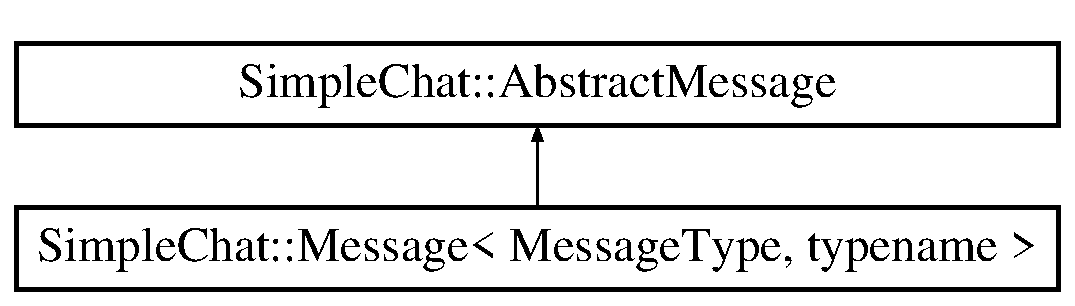
\includegraphics[height=2.000000cm]{classSimpleChat_1_1AbstractMessage}
\end{center}
\end{figure}
\subsection*{Public Member Functions}
\begin{DoxyCompactItemize}
\item 
\hypertarget{classSimpleChat_1_1AbstractMessage_a6920d6c85c58836df0231dc928a7e89d}{virtual std\-::string {\bfseries serialize} ()=0}\label{classSimpleChat_1_1AbstractMessage_a6920d6c85c58836df0231dc928a7e89d}

\item 
\hypertarget{classSimpleChat_1_1AbstractMessage_adccc53225d21696f0c55fb336ce8f2b9}{virtual int {\bfseries type} ()=0}\label{classSimpleChat_1_1AbstractMessage_adccc53225d21696f0c55fb336ce8f2b9}

\item 
\hypertarget{classSimpleChat_1_1AbstractMessage_a626a708cc046249083273620d8db74d8}{virtual bool {\bfseries is\-Initialized} ()=0}\label{classSimpleChat_1_1AbstractMessage_a626a708cc046249083273620d8db74d8}

\item 
\hypertarget{classSimpleChat_1_1AbstractMessage_a7fae15db18e8572a7c58651b724636bb}{virtual std\-::unique\-\_\-ptr\\*
$<$ \hyperlink{classSimpleChat_1_1AbstractMessage}{Abstract\-Message} $>$ {\bfseries clone} ()=0}\label{classSimpleChat_1_1AbstractMessage_a7fae15db18e8572a7c58651b724636bb}

\end{DoxyCompactItemize}


The documentation for this class was generated from the following file\-:\begin{DoxyCompactItemize}
\item 
chatlib/communication/Abstract\-Message.\-h\end{DoxyCompactItemize}

\hypertarget{classSimpleChat_1_1AuthChatCommand}{\section{Simple\-Chat\-:\-:Auth\-Chat\-Command Class Reference}
\label{classSimpleChat_1_1AuthChatCommand}\index{Simple\-Chat\-::\-Auth\-Chat\-Command@{Simple\-Chat\-::\-Auth\-Chat\-Command}}
}
Inheritance diagram for Simple\-Chat\-:\-:Auth\-Chat\-Command\-:\begin{figure}[H]
\begin{center}
\leavevmode
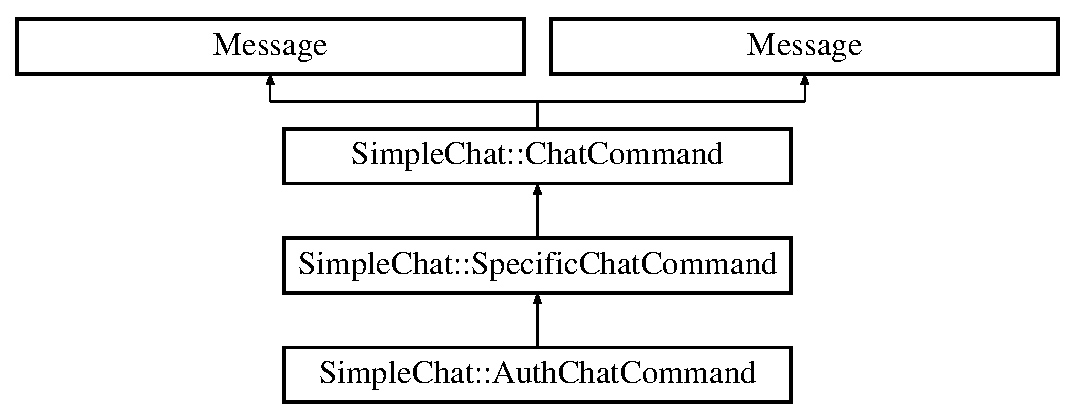
\includegraphics[height=4.000000cm]{classSimpleChat_1_1AuthChatCommand}
\end{center}
\end{figure}
\subsection*{Public Member Functions}
\begin{DoxyCompactItemize}
\item 
void \hyperlink{classSimpleChat_1_1AuthChatCommand_ae1cefe2b498c5829d9db584c25473d65}{insert\-Data} (const std\-::vector$<$ std\-::string $>$ \&arguments) override
\end{DoxyCompactItemize}
\subsection*{Additional Inherited Members}


\subsection{Member Function Documentation}
\hypertarget{classSimpleChat_1_1AuthChatCommand_ae1cefe2b498c5829d9db584c25473d65}{\index{Simple\-Chat\-::\-Auth\-Chat\-Command@{Simple\-Chat\-::\-Auth\-Chat\-Command}!insert\-Data@{insert\-Data}}
\index{insert\-Data@{insert\-Data}!SimpleChat::AuthChatCommand@{Simple\-Chat\-::\-Auth\-Chat\-Command}}
\subsubsection[{insert\-Data}]{\setlength{\rightskip}{0pt plus 5cm}void Simple\-Chat\-::\-Auth\-Chat\-Command\-::insert\-Data (
\begin{DoxyParamCaption}
\item[{const std\-::vector$<$ std\-::string $>$ \&}]{arguments}
\end{DoxyParamCaption}
)\hspace{0.3cm}{\ttfamily [override]}, {\ttfamily [virtual]}}}\label{classSimpleChat_1_1AuthChatCommand_ae1cefe2b498c5829d9db584c25473d65}
argument is a password 

Implements \hyperlink{classSimpleChat_1_1SpecificChatCommand}{Simple\-Chat\-::\-Specific\-Chat\-Command}.



The documentation for this class was generated from the following files\-:\begin{DoxyCompactItemize}
\item 
chatlib/chat/commands/Auth\-Chat\-Command.\-h\item 
chatlib/chat/commands/Auth\-Chat\-Command.\-cpp\end{DoxyCompactItemize}

\hypertarget{classSimpleChat_1_1ChatAuthorize}{\section{Simple\-Chat\-:\-:Chat\-Authorize Class Reference}
\label{classSimpleChat_1_1ChatAuthorize}\index{Simple\-Chat\-::\-Chat\-Authorize@{Simple\-Chat\-::\-Chat\-Authorize}}
}
Inheritance diagram for Simple\-Chat\-:\-:Chat\-Authorize\-:\begin{figure}[H]
\begin{center}
\leavevmode
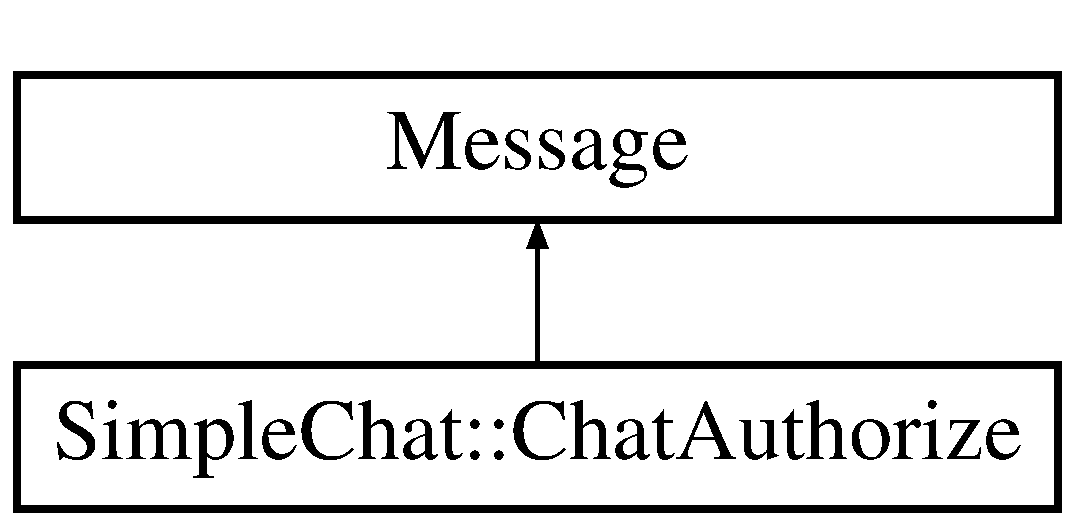
\includegraphics[height=2.000000cm]{classSimpleChat_1_1ChatAuthorize}
\end{center}
\end{figure}
\subsection*{Public Member Functions}
\begin{DoxyCompactItemize}
\item 
\hypertarget{classSimpleChat_1_1ChatAuthorize_abc1fac7df5e5e595ff6cfc111e307bf7}{{\bfseries Chat\-Authorize} (const \hyperlink{classSimpleChat_1_1ChatAuthorize}{Chat\-Authorize} \&from)}\label{classSimpleChat_1_1ChatAuthorize_abc1fac7df5e5e595ff6cfc111e307bf7}

\item 
\hypertarget{classSimpleChat_1_1ChatAuthorize_a52df37784f8170609af4c5dd14bc1315}{\hyperlink{classSimpleChat_1_1ChatAuthorize}{Chat\-Authorize} \& {\bfseries operator=} (const \hyperlink{classSimpleChat_1_1ChatAuthorize}{Chat\-Authorize} \&from)}\label{classSimpleChat_1_1ChatAuthorize_a52df37784f8170609af4c5dd14bc1315}

\item 
\hypertarget{classSimpleChat_1_1ChatAuthorize_ae41c4e349ea250cf7e0b217df18297d1}{const \\*
\-::google\-::protobuf\-::\-Unknown\-Field\-Set \& {\bfseries unknown\-\_\-fields} () const }\label{classSimpleChat_1_1ChatAuthorize_ae41c4e349ea250cf7e0b217df18297d1}

\item 
\hypertarget{classSimpleChat_1_1ChatAuthorize_ac1855f10260362d22995aa8db2ad55d3}{inline\-::google\-::protobuf\-::\-Unknown\-Field\-Set $\ast$ {\bfseries mutable\-\_\-unknown\-\_\-fields} ()}\label{classSimpleChat_1_1ChatAuthorize_ac1855f10260362d22995aa8db2ad55d3}

\item 
\hypertarget{classSimpleChat_1_1ChatAuthorize_a21801c93fdbf77f682b696414a61fd90}{void {\bfseries Swap} (\hyperlink{classSimpleChat_1_1ChatAuthorize}{Chat\-Authorize} $\ast$other)}\label{classSimpleChat_1_1ChatAuthorize_a21801c93fdbf77f682b696414a61fd90}

\item 
\hypertarget{classSimpleChat_1_1ChatAuthorize_aa001d0e9561d6311b94616b7bdec0caf}{\hyperlink{classSimpleChat_1_1ChatAuthorize}{Chat\-Authorize} $\ast$ {\bfseries New} () const }\label{classSimpleChat_1_1ChatAuthorize_aa001d0e9561d6311b94616b7bdec0caf}

\item 
\hypertarget{classSimpleChat_1_1ChatAuthorize_aa50fa8e8e9f52ec6f0185aea43e30dda}{\hyperlink{classSimpleChat_1_1ChatAuthorize}{Chat\-Authorize} $\ast$ {\bfseries New} (\-::google\-::protobuf\-::\-Arena $\ast$arena) const }\label{classSimpleChat_1_1ChatAuthorize_aa50fa8e8e9f52ec6f0185aea43e30dda}

\item 
\hypertarget{classSimpleChat_1_1ChatAuthorize_a03ac64a3503ed199f3dda6fd0f037917}{void {\bfseries Copy\-From} (const \-::google\-::protobuf\-::\-Message \&from)}\label{classSimpleChat_1_1ChatAuthorize_a03ac64a3503ed199f3dda6fd0f037917}

\item 
\hypertarget{classSimpleChat_1_1ChatAuthorize_a48fdfb8dc96cd091b9fc233b76d0374d}{void {\bfseries Merge\-From} (const \-::google\-::protobuf\-::\-Message \&from)}\label{classSimpleChat_1_1ChatAuthorize_a48fdfb8dc96cd091b9fc233b76d0374d}

\item 
\hypertarget{classSimpleChat_1_1ChatAuthorize_ab1e8a628454d4fff99e9cb61f528dee8}{void {\bfseries Copy\-From} (const \hyperlink{classSimpleChat_1_1ChatAuthorize}{Chat\-Authorize} \&from)}\label{classSimpleChat_1_1ChatAuthorize_ab1e8a628454d4fff99e9cb61f528dee8}

\item 
\hypertarget{classSimpleChat_1_1ChatAuthorize_ac5af381dc9144fb5d8f24a6e167f692d}{void {\bfseries Merge\-From} (const \hyperlink{classSimpleChat_1_1ChatAuthorize}{Chat\-Authorize} \&from)}\label{classSimpleChat_1_1ChatAuthorize_ac5af381dc9144fb5d8f24a6e167f692d}

\item 
\hypertarget{classSimpleChat_1_1ChatAuthorize_a8b7a933d77521062b037117975c47adc}{void {\bfseries Clear} ()}\label{classSimpleChat_1_1ChatAuthorize_a8b7a933d77521062b037117975c47adc}

\item 
\hypertarget{classSimpleChat_1_1ChatAuthorize_a7b1b8e15a6224defe50585275db9eb16}{bool {\bfseries Is\-Initialized} () const }\label{classSimpleChat_1_1ChatAuthorize_a7b1b8e15a6224defe50585275db9eb16}

\item 
\hypertarget{classSimpleChat_1_1ChatAuthorize_af4891a6c8d555414efce16a1b5899de5}{int {\bfseries Byte\-Size} () const }\label{classSimpleChat_1_1ChatAuthorize_af4891a6c8d555414efce16a1b5899de5}

\item 
\hypertarget{classSimpleChat_1_1ChatAuthorize_a1d571702eb25817fb6f90a888ab8096a}{bool {\bfseries Merge\-Partial\-From\-Coded\-Stream} (\-::google\-::protobuf\-::io\-::\-Coded\-Input\-Stream $\ast$input)}\label{classSimpleChat_1_1ChatAuthorize_a1d571702eb25817fb6f90a888ab8096a}

\item 
\hypertarget{classSimpleChat_1_1ChatAuthorize_a302ac1ec2a227fa677ca01235986f56b}{void {\bfseries Serialize\-With\-Cached\-Sizes} (\-::google\-::protobuf\-::io\-::\-Coded\-Output\-Stream $\ast$output) const }\label{classSimpleChat_1_1ChatAuthorize_a302ac1ec2a227fa677ca01235986f56b}

\item 
\hypertarget{classSimpleChat_1_1ChatAuthorize_a8685044ee854f95eb3d660c55451f435}{\-::google\-::protobuf\-::uint8 $\ast$ {\bfseries Serialize\-With\-Cached\-Sizes\-To\-Array} (\-::google\-::protobuf\-::uint8 $\ast$output) const }\label{classSimpleChat_1_1ChatAuthorize_a8685044ee854f95eb3d660c55451f435}

\item 
\hypertarget{classSimpleChat_1_1ChatAuthorize_a864e12f84de95a97d9cdd518d34c0f39}{int {\bfseries Get\-Cached\-Size} () const }\label{classSimpleChat_1_1ChatAuthorize_a864e12f84de95a97d9cdd518d34c0f39}

\item 
\hypertarget{classSimpleChat_1_1ChatAuthorize_ac4c9d359759eb147f1359240de4642d4}{\-::google\-::protobuf\-::\-Metadata {\bfseries Get\-Metadata} () const }\label{classSimpleChat_1_1ChatAuthorize_ac4c9d359759eb147f1359240de4642d4}

\item 
\hypertarget{classSimpleChat_1_1ChatAuthorize_a3565bd9c13fd17b4b6da62671f705da0}{bool {\bfseries has\-\_\-from} () const }\label{classSimpleChat_1_1ChatAuthorize_a3565bd9c13fd17b4b6da62671f705da0}

\item 
\hypertarget{classSimpleChat_1_1ChatAuthorize_af38007e02776a313355a80bbdcded35f}{void {\bfseries clear\-\_\-from} ()}\label{classSimpleChat_1_1ChatAuthorize_af38007e02776a313355a80bbdcded35f}

\item 
\hypertarget{classSimpleChat_1_1ChatAuthorize_a37ea94200024dfea736825e2490dd78d}{const \-::\hyperlink{classSimpleChat_1_1ChatTarget}{Simple\-Chat\-::\-Chat\-Target} \& {\bfseries from} () const }\label{classSimpleChat_1_1ChatAuthorize_a37ea94200024dfea736825e2490dd78d}

\item 
\hypertarget{classSimpleChat_1_1ChatAuthorize_a2f956f0a1cfe5252e3c1a57a79ee2d34}{\-::\hyperlink{classSimpleChat_1_1ChatTarget}{Simple\-Chat\-::\-Chat\-Target} $\ast$ {\bfseries mutable\-\_\-from} ()}\label{classSimpleChat_1_1ChatAuthorize_a2f956f0a1cfe5252e3c1a57a79ee2d34}

\item 
\hypertarget{classSimpleChat_1_1ChatAuthorize_a7627ace10e743451b8a00be03f9cbbb3}{\-::\hyperlink{classSimpleChat_1_1ChatTarget}{Simple\-Chat\-::\-Chat\-Target} $\ast$ {\bfseries release\-\_\-from} ()}\label{classSimpleChat_1_1ChatAuthorize_a7627ace10e743451b8a00be03f9cbbb3}

\item 
\hypertarget{classSimpleChat_1_1ChatAuthorize_a6fbbc89d79068159644f157b15eeaa37}{void {\bfseries set\-\_\-allocated\-\_\-from} (\-::\hyperlink{classSimpleChat_1_1ChatTarget}{Simple\-Chat\-::\-Chat\-Target} $\ast$from)}\label{classSimpleChat_1_1ChatAuthorize_a6fbbc89d79068159644f157b15eeaa37}

\item 
\hypertarget{classSimpleChat_1_1ChatAuthorize_a5a831a5ec05ba2111daad19523cab731}{bool {\bfseries has\-\_\-password} () const }\label{classSimpleChat_1_1ChatAuthorize_a5a831a5ec05ba2111daad19523cab731}

\item 
\hypertarget{classSimpleChat_1_1ChatAuthorize_acd5a80ea6900f8dc3a8665e155b09d87}{void {\bfseries clear\-\_\-password} ()}\label{classSimpleChat_1_1ChatAuthorize_acd5a80ea6900f8dc3a8665e155b09d87}

\item 
\hypertarget{classSimpleChat_1_1ChatAuthorize_a8c6b4148752b1f1634cef898ffdb47ef}{const \-::std\-::string \& {\bfseries password} () const }\label{classSimpleChat_1_1ChatAuthorize_a8c6b4148752b1f1634cef898ffdb47ef}

\item 
\hypertarget{classSimpleChat_1_1ChatAuthorize_abd5112e528acd7ebadbe4a1582638f4d}{void {\bfseries set\-\_\-password} (const \-::std\-::string \&value)}\label{classSimpleChat_1_1ChatAuthorize_abd5112e528acd7ebadbe4a1582638f4d}

\item 
\hypertarget{classSimpleChat_1_1ChatAuthorize_a2756e5b59b6f42d2d16d621bc6d0414b}{void {\bfseries set\-\_\-password} (const char $\ast$value)}\label{classSimpleChat_1_1ChatAuthorize_a2756e5b59b6f42d2d16d621bc6d0414b}

\item 
\hypertarget{classSimpleChat_1_1ChatAuthorize_aaa5d3d2838522bf1be1bcc2f341196f5}{void {\bfseries set\-\_\-password} (const char $\ast$value, size\-\_\-t size)}\label{classSimpleChat_1_1ChatAuthorize_aaa5d3d2838522bf1be1bcc2f341196f5}

\item 
\hypertarget{classSimpleChat_1_1ChatAuthorize_a388caaa541281ef4444d575b152b603d}{\-::std\-::string $\ast$ {\bfseries mutable\-\_\-password} ()}\label{classSimpleChat_1_1ChatAuthorize_a388caaa541281ef4444d575b152b603d}

\item 
\hypertarget{classSimpleChat_1_1ChatAuthorize_a52ce150b76009f5ac35cf1ef1fd456e1}{\-::std\-::string $\ast$ {\bfseries release\-\_\-password} ()}\label{classSimpleChat_1_1ChatAuthorize_a52ce150b76009f5ac35cf1ef1fd456e1}

\item 
\hypertarget{classSimpleChat_1_1ChatAuthorize_a631b03ab4c754ef493b9e4360f38881c}{void {\bfseries set\-\_\-allocated\-\_\-password} (\-::std\-::string $\ast$password)}\label{classSimpleChat_1_1ChatAuthorize_a631b03ab4c754ef493b9e4360f38881c}

\end{DoxyCompactItemize}
\subsection*{Static Public Member Functions}
\begin{DoxyCompactItemize}
\item 
\hypertarget{classSimpleChat_1_1ChatAuthorize_a73777df8cfd92e3ea82f27d7fdb2b0e9}{static const \\*
\-::google\-::protobuf\-::\-Descriptor $\ast$ {\bfseries descriptor} ()}\label{classSimpleChat_1_1ChatAuthorize_a73777df8cfd92e3ea82f27d7fdb2b0e9}

\item 
\hypertarget{classSimpleChat_1_1ChatAuthorize_adb0513feb6b35f1ded55c3af00a6d2d8}{static const \hyperlink{classSimpleChat_1_1ChatAuthorize}{Chat\-Authorize} \& {\bfseries default\-\_\-instance} ()}\label{classSimpleChat_1_1ChatAuthorize_adb0513feb6b35f1ded55c3af00a6d2d8}

\end{DoxyCompactItemize}
\subsection*{Static Public Attributes}
\begin{DoxyCompactItemize}
\item 
\hypertarget{classSimpleChat_1_1ChatAuthorize_ac40beded29445d79e301f53f81e2c153}{static const int {\bfseries k\-From\-Field\-Number} = 1}\label{classSimpleChat_1_1ChatAuthorize_ac40beded29445d79e301f53f81e2c153}

\item 
\hypertarget{classSimpleChat_1_1ChatAuthorize_ad1fdee1f90e42f300135651f9440fbf4}{static const int {\bfseries k\-Password\-Field\-Number} = 2}\label{classSimpleChat_1_1ChatAuthorize_ad1fdee1f90e42f300135651f9440fbf4}

\end{DoxyCompactItemize}
\subsection*{Friends}
\begin{DoxyCompactItemize}
\item 
\hypertarget{classSimpleChat_1_1ChatAuthorize_ab0d9593aa41361f04ab91f917ef9ec0e}{void {\bfseries protobuf\-\_\-\-Add\-Desc\-\_\-\-Chat\-Message\-\_\-2eproto} ()}\label{classSimpleChat_1_1ChatAuthorize_ab0d9593aa41361f04ab91f917ef9ec0e}

\item 
\hypertarget{classSimpleChat_1_1ChatAuthorize_a4ca7b2c64786782406ca69f6ba39ccb2}{void {\bfseries protobuf\-\_\-\-Assign\-Desc\-\_\-\-Chat\-Message\-\_\-2eproto} ()}\label{classSimpleChat_1_1ChatAuthorize_a4ca7b2c64786782406ca69f6ba39ccb2}

\item 
\hypertarget{classSimpleChat_1_1ChatAuthorize_a78726b79d52a130a50d7670a5c0238fc}{void {\bfseries protobuf\-\_\-\-Shutdown\-File\-\_\-\-Chat\-Message\-\_\-2eproto} ()}\label{classSimpleChat_1_1ChatAuthorize_a78726b79d52a130a50d7670a5c0238fc}

\end{DoxyCompactItemize}


The documentation for this class was generated from the following file\-:\begin{DoxyCompactItemize}
\item 
shared/proto/Chat\-Message.\-pb.\-h\end{DoxyCompactItemize}

\hypertarget{classSimpleChat_1_1ChatClient}{\section{Simple\-Chat\-:\-:Chat\-Client Class Reference}
\label{classSimpleChat_1_1ChatClient}\index{Simple\-Chat\-::\-Chat\-Client@{Simple\-Chat\-::\-Chat\-Client}}
}
Inheritance diagram for Simple\-Chat\-:\-:Chat\-Client\-:\begin{figure}[H]
\begin{center}
\leavevmode
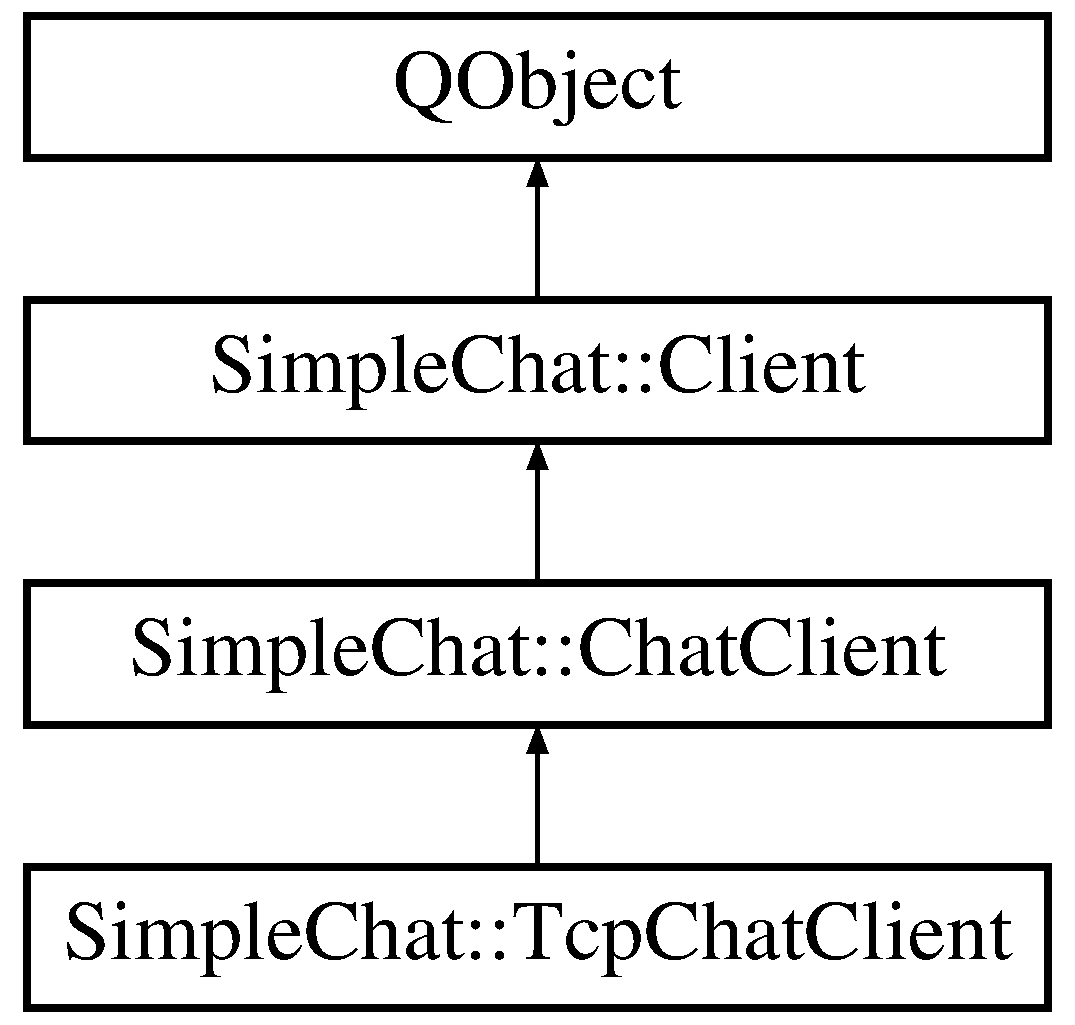
\includegraphics[height=4.000000cm]{classSimpleChat_1_1ChatClient}
\end{center}
\end{figure}
\subsection*{Public Member Functions}
\begin{DoxyCompactItemize}
\item 
\hypertarget{classSimpleChat_1_1ChatClient_a3ca3b550ca39f0e467568d47c02528e0}{virtual bool {\bfseries send\-Command} (const std\-::string \&command) override}\label{classSimpleChat_1_1ChatClient_a3ca3b550ca39f0e467568d47c02528e0}

\item 
\hypertarget{classSimpleChat_1_1ChatClient_a0b36d2b71249b8aa1b6a57e6a0e2c6e8}{virtual void {\bfseries send\-Message} (const std\-::string \&text, const std\-::string \&target=\char`\"{}\char`\"{}) override}\label{classSimpleChat_1_1ChatClient_a0b36d2b71249b8aa1b6a57e6a0e2c6e8}

\item 
\hypertarget{classSimpleChat_1_1ChatClient_a3cda3fd789bd6862bdfa0409b09f43aa}{virtual void {\bfseries handle\-Untyped\-Message} (const \hyperlink{classSimpleChat_1_1MessageDeserializer}{Message\-Deserializer} \&deserializer) override}\label{classSimpleChat_1_1ChatClient_a3cda3fd789bd6862bdfa0409b09f43aa}

\item 
\hypertarget{classSimpleChat_1_1ChatClient_aef22a40abcc5c04daa080146e9f8e493}{virtual void {\bfseries handle\-Message} (std\-::unique\-\_\-ptr$<$ \hyperlink{classSimpleChat_1_1UserJoinResponse}{User\-Join\-Response} $>$ join\-Response) override}\label{classSimpleChat_1_1ChatClient_aef22a40abcc5c04daa080146e9f8e493}

\item 
\hypertarget{classSimpleChat_1_1ChatClient_af5dddaded163059d6f77531c368d52d7}{virtual void {\bfseries handle\-Message} (std\-::unique\-\_\-ptr$<$ \hyperlink{classSimpleChat_1_1UserListResponse}{User\-List\-Response} $>$ list\-Response) override}\label{classSimpleChat_1_1ChatClient_af5dddaded163059d6f77531c368d52d7}

\item 
virtual void \hyperlink{classSimpleChat_1_1ChatClient_a432edc64a95f480235df3d1d7f55fbce}{handle\-Message} (std\-::unique\-\_\-ptr$<$ \hyperlink{classSimpleChat_1_1UserChange}{User\-Change} $>$ user\-Change) override
\item 
\hypertarget{classSimpleChat_1_1ChatClient_ae9c20505289ce814b27299cfb3a7db77}{virtual void {\bfseries handle\-Message} (std\-::unique\-\_\-ptr$<$ \hyperlink{classSimpleChat_1_1ChatMessage}{Chat\-Message} $>$ chat\-Message) override}\label{classSimpleChat_1_1ChatClient_ae9c20505289ce814b27299cfb3a7db77}

\item 
\hypertarget{classSimpleChat_1_1ChatClient_a5d5645f4e9f2915b273b7cb60bbc61de}{virtual void {\bfseries handle\-Message} (std\-::unique\-\_\-ptr$<$ \hyperlink{classSimpleChat_1_1ChatroomChange}{Chatroom\-Change} $>$ chatroom\-Change) override}\label{classSimpleChat_1_1ChatClient_a5d5645f4e9f2915b273b7cb60bbc61de}

\item 
\hypertarget{classSimpleChat_1_1ChatClient_a5022c5d4eced511bcd127c53e1442b21}{virtual void {\bfseries handle\-Message} (std\-::unique\-\_\-ptr$<$ \hyperlink{classSimpleChat_1_1GenericChatResponse}{Generic\-Chat\-Response} $>$ response) override}\label{classSimpleChat_1_1ChatClient_a5022c5d4eced511bcd127c53e1442b21}

\item 
\hypertarget{classSimpleChat_1_1ChatClient_ae7f07c0ce640dc5d379914ecab79af3c}{virtual bool {\bfseries connect\-To\-Server} ()=0}\label{classSimpleChat_1_1ChatClient_ae7f07c0ce640dc5d379914ecab79af3c}

\item 
\hypertarget{classSimpleChat_1_1ChatClient_ade4303abd1dc4a069b088976d310f696}{virtual void {\bfseries join} ()=0}\label{classSimpleChat_1_1ChatClient_ade4303abd1dc4a069b088976d310f696}

\item 
\hypertarget{classSimpleChat_1_1ChatClient_a7ab65b6cf92b058242c9a163afa89fd8}{virtual void {\bfseries request\-User\-List} ()=0}\label{classSimpleChat_1_1ChatClient_a7ab65b6cf92b058242c9a163afa89fd8}

\item 
\hypertarget{classSimpleChat_1_1ChatClient_a15fc2e659a8d36d3012127e0abf37b8f}{std\-::shared\-\_\-ptr$<$ \hyperlink{classSimpleChat_1_1Chatroom}{Chatroom} $>$ {\bfseries chatroom} ()}\label{classSimpleChat_1_1ChatClient_a15fc2e659a8d36d3012127e0abf37b8f}

\item 
\hypertarget{classSimpleChat_1_1ChatClient_a321f3bb9f9254740731b22babe4bc744}{virtual std\-::string {\bfseries name} () override}\label{classSimpleChat_1_1ChatClient_a321f3bb9f9254740731b22babe4bc744}

\end{DoxyCompactItemize}
\subsection*{Protected Member Functions}
\begin{DoxyCompactItemize}
\item 
\hypertarget{classSimpleChat_1_1ChatClient_a5ded6a9e1c646519402fac5d04d68859}{virtual bool {\bfseries send\-Any\-Message} (std\-::unique\-\_\-ptr$<$ \hyperlink{classSimpleChat_1_1AbstractMessage}{Abstract\-Message} $>$ message) override=0}\label{classSimpleChat_1_1ChatClient_a5ded6a9e1c646519402fac5d04d68859}

\item 
\hypertarget{classSimpleChat_1_1ChatClient_a6e715c23071858bc5c67b7146f9f18eb}{virtual bool {\bfseries is\-Connected} () override=0}\label{classSimpleChat_1_1ChatClient_a6e715c23071858bc5c67b7146f9f18eb}

\item 
\hypertarget{classSimpleChat_1_1ChatClient_a5a949c5938522983e0fee9d99fd10cb5}{virtual \hyperlink{classSimpleChat_1_1ChatConnection}{Chat\-Connection} $\ast$ {\bfseries connection} () override=0}\label{classSimpleChat_1_1ChatClient_a5a949c5938522983e0fee9d99fd10cb5}

\item 
\hypertarget{classSimpleChat_1_1ChatClient_a7284056b4774b6c04f11dc289f93805f}{virtual void {\bfseries chatee\-Joined} (const std\-::string \&name) override=0}\label{classSimpleChat_1_1ChatClient_a7284056b4774b6c04f11dc289f93805f}

\item 
\hypertarget{classSimpleChat_1_1ChatClient_a48b62cbb729cd0283f288caf6645d337}{virtual void {\bfseries chatee\-Left} (const std\-::string \&name) override=0}\label{classSimpleChat_1_1ChatClient_a48b62cbb729cd0283f288caf6645d337}

\item 
\hypertarget{classSimpleChat_1_1ChatClient_a13e625d13df8858301c14170292a9503}{virtual void {\bfseries chat\-Motd\-Changed} (const std\-::string \&motd) override=0}\label{classSimpleChat_1_1ChatClient_a13e625d13df8858301c14170292a9503}

\item 
\hypertarget{classSimpleChat_1_1ChatClient_aac3558bb326904aee565d90cbd95e2c6}{virtual void {\bfseries chat\-Info\-Received} (const std\-::string \&info) override=0}\label{classSimpleChat_1_1ChatClient_aac3558bb326904aee565d90cbd95e2c6}

\item 
\hypertarget{classSimpleChat_1_1ChatClient_ac56ed6f591d5a4843b1b0e017ed3ca2e}{virtual void {\bfseries chat\-Message\-Received} (const std\-::string \&text, const std\-::string \&from, const std\-::string \&target) override=0}\label{classSimpleChat_1_1ChatClient_ac56ed6f591d5a4843b1b0e017ed3ca2e}

\item 
\hypertarget{classSimpleChat_1_1ChatClient_a5591d713d7df3fe488c2df7b9b9d869a}{virtual void {\bfseries refresh\-Chatee\-List} () override=0}\label{classSimpleChat_1_1ChatClient_a5591d713d7df3fe488c2df7b9b9d869a}

\end{DoxyCompactItemize}
\subsection*{Protected Attributes}
\begin{DoxyCompactItemize}
\item 
\hypertarget{classSimpleChat_1_1ChatClient_ab70046d19ca2c6cfc0ed522405fcbeaa}{std\-::string {\bfseries client\-Name\-\_\-}}\label{classSimpleChat_1_1ChatClient_ab70046d19ca2c6cfc0ed522405fcbeaa}

\item 
\hypertarget{classSimpleChat_1_1ChatClient_a46b558b9a65e8699d67ce7bda11681f0}{std\-::shared\-\_\-ptr$<$ \hyperlink{classSimpleChat_1_1Chatroom}{Chatroom} $>$ {\bfseries chatroom\-\_\-}}\label{classSimpleChat_1_1ChatClient_a46b558b9a65e8699d67ce7bda11681f0}

\end{DoxyCompactItemize}
\subsection*{Additional Inherited Members}


\subsection{Member Function Documentation}
\hypertarget{classSimpleChat_1_1ChatClient_a432edc64a95f480235df3d1d7f55fbce}{\index{Simple\-Chat\-::\-Chat\-Client@{Simple\-Chat\-::\-Chat\-Client}!handle\-Message@{handle\-Message}}
\index{handle\-Message@{handle\-Message}!SimpleChat::ChatClient@{Simple\-Chat\-::\-Chat\-Client}}
\subsubsection[{handle\-Message}]{\setlength{\rightskip}{0pt plus 5cm}void Simple\-Chat\-::\-Chat\-Client\-::handle\-Message (
\begin{DoxyParamCaption}
\item[{std\-::unique\-\_\-ptr$<$ {\bf User\-Change} $>$}]{user\-Change}
\end{DoxyParamCaption}
)\hspace{0.3cm}{\ttfamily [override]}, {\ttfamily [virtual]}}}\label{classSimpleChat_1_1ChatClient_a432edc64a95f480235df3d1d7f55fbce}
check for join first because chatee doesn't exist yet 

Implements \hyperlink{classSimpleChat_1_1Client}{Simple\-Chat\-::\-Client}.



The documentation for this class was generated from the following files\-:\begin{DoxyCompactItemize}
\item 
chatlib/client/Chat\-Client.\-h\item 
chatlib/client/Chat\-Client.\-cpp\end{DoxyCompactItemize}

\hypertarget{classSimpleChat_1_1ChatCommand}{\section{Simple\-Chat\-:\-:Chat\-Command Class Reference}
\label{classSimpleChat_1_1ChatCommand}\index{Simple\-Chat\-::\-Chat\-Command@{Simple\-Chat\-::\-Chat\-Command}}
}
Inheritance diagram for Simple\-Chat\-:\-:Chat\-Command\-:\begin{figure}[H]
\begin{center}
\leavevmode
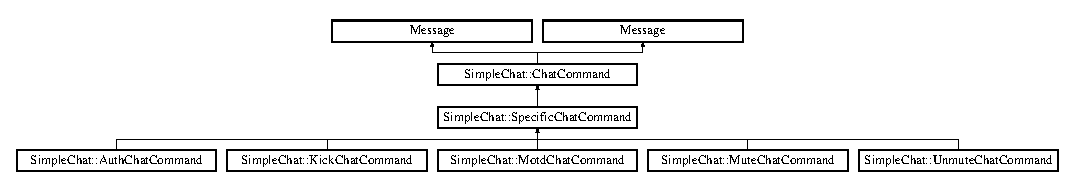
\includegraphics[height=2.074074cm]{classSimpleChat_1_1ChatCommand}
\end{center}
\end{figure}
\subsection*{Public Member Functions}
\begin{DoxyCompactItemize}
\item 
\hypertarget{classSimpleChat_1_1ChatCommand_aa16520371fefabad5f42be66c2166115}{{\bfseries Chat\-Command} (const \hyperlink{classSimpleChat_1_1ChatCommand}{Chat\-Command} \&from)}\label{classSimpleChat_1_1ChatCommand_aa16520371fefabad5f42be66c2166115}

\item 
\hypertarget{classSimpleChat_1_1ChatCommand_a7c066b1b1e8df8fa4cbdcada306b5131}{\hyperlink{classSimpleChat_1_1ChatCommand}{Chat\-Command} \& {\bfseries operator=} (const \hyperlink{classSimpleChat_1_1ChatCommand}{Chat\-Command} \&from)}\label{classSimpleChat_1_1ChatCommand_a7c066b1b1e8df8fa4cbdcada306b5131}

\item 
\hypertarget{classSimpleChat_1_1ChatCommand_afc3fdc2a7378b379d0b1b5bd96c15b84}{const \\*
\-::google\-::protobuf\-::\-Unknown\-Field\-Set \& {\bfseries unknown\-\_\-fields} () const }\label{classSimpleChat_1_1ChatCommand_afc3fdc2a7378b379d0b1b5bd96c15b84}

\item 
\hypertarget{classSimpleChat_1_1ChatCommand_aab03f63fc0707e0f99354f22ba7d24a9}{inline\-::google\-::protobuf\-::\-Unknown\-Field\-Set $\ast$ {\bfseries mutable\-\_\-unknown\-\_\-fields} ()}\label{classSimpleChat_1_1ChatCommand_aab03f63fc0707e0f99354f22ba7d24a9}

\item 
\hypertarget{classSimpleChat_1_1ChatCommand_a089731c3f481fc59720de75bb57d0453}{void {\bfseries Swap} (\hyperlink{classSimpleChat_1_1ChatCommand}{Chat\-Command} $\ast$other)}\label{classSimpleChat_1_1ChatCommand_a089731c3f481fc59720de75bb57d0453}

\item 
\hypertarget{classSimpleChat_1_1ChatCommand_abd47580fa1ed63285ff861c67bac13d7}{\hyperlink{classSimpleChat_1_1ChatCommand}{Chat\-Command} $\ast$ {\bfseries New} () const }\label{classSimpleChat_1_1ChatCommand_abd47580fa1ed63285ff861c67bac13d7}

\item 
\hypertarget{classSimpleChat_1_1ChatCommand_a4a1aaeaf97d2027fcb439262a6fa2641}{\hyperlink{classSimpleChat_1_1ChatCommand}{Chat\-Command} $\ast$ {\bfseries New} (\-::google\-::protobuf\-::\-Arena $\ast$arena) const }\label{classSimpleChat_1_1ChatCommand_a4a1aaeaf97d2027fcb439262a6fa2641}

\item 
\hypertarget{classSimpleChat_1_1ChatCommand_a87d01f257540ddb198889eb5ac90b9e8}{void {\bfseries Copy\-From} (const \-::google\-::protobuf\-::\-Message \&from)}\label{classSimpleChat_1_1ChatCommand_a87d01f257540ddb198889eb5ac90b9e8}

\item 
\hypertarget{classSimpleChat_1_1ChatCommand_aa58b45138751c053e0064dcccb096a4c}{void {\bfseries Merge\-From} (const \-::google\-::protobuf\-::\-Message \&from)}\label{classSimpleChat_1_1ChatCommand_aa58b45138751c053e0064dcccb096a4c}

\item 
\hypertarget{classSimpleChat_1_1ChatCommand_ae9451f271b99462bfa76a5071a2be90c}{void {\bfseries Copy\-From} (const \hyperlink{classSimpleChat_1_1ChatCommand}{Chat\-Command} \&from)}\label{classSimpleChat_1_1ChatCommand_ae9451f271b99462bfa76a5071a2be90c}

\item 
\hypertarget{classSimpleChat_1_1ChatCommand_aa456dbbffa7e3944bb0c52c439886e03}{void {\bfseries Merge\-From} (const \hyperlink{classSimpleChat_1_1ChatCommand}{Chat\-Command} \&from)}\label{classSimpleChat_1_1ChatCommand_aa456dbbffa7e3944bb0c52c439886e03}

\item 
\hypertarget{classSimpleChat_1_1ChatCommand_a22dd73cd4eb8e470615d8fdc90de3136}{void {\bfseries Clear} ()}\label{classSimpleChat_1_1ChatCommand_a22dd73cd4eb8e470615d8fdc90de3136}

\item 
\hypertarget{classSimpleChat_1_1ChatCommand_abe7098c37325708404ddd6571727b81c}{bool {\bfseries Is\-Initialized} () const }\label{classSimpleChat_1_1ChatCommand_abe7098c37325708404ddd6571727b81c}

\item 
\hypertarget{classSimpleChat_1_1ChatCommand_a22213d9b1e8634eba2e75f36d068db12}{int {\bfseries Byte\-Size} () const }\label{classSimpleChat_1_1ChatCommand_a22213d9b1e8634eba2e75f36d068db12}

\item 
\hypertarget{classSimpleChat_1_1ChatCommand_acc63785a17c5e8f667c3c0287f54a144}{bool {\bfseries Merge\-Partial\-From\-Coded\-Stream} (\-::google\-::protobuf\-::io\-::\-Coded\-Input\-Stream $\ast$input)}\label{classSimpleChat_1_1ChatCommand_acc63785a17c5e8f667c3c0287f54a144}

\item 
\hypertarget{classSimpleChat_1_1ChatCommand_a41bc3d65c65cc85132c8d246eac09123}{void {\bfseries Serialize\-With\-Cached\-Sizes} (\-::google\-::protobuf\-::io\-::\-Coded\-Output\-Stream $\ast$output) const }\label{classSimpleChat_1_1ChatCommand_a41bc3d65c65cc85132c8d246eac09123}

\item 
\hypertarget{classSimpleChat_1_1ChatCommand_aed35c954d2fd083aa0fca4a8757e35ca}{\-::google\-::protobuf\-::uint8 $\ast$ {\bfseries Serialize\-With\-Cached\-Sizes\-To\-Array} (\-::google\-::protobuf\-::uint8 $\ast$output) const }\label{classSimpleChat_1_1ChatCommand_aed35c954d2fd083aa0fca4a8757e35ca}

\item 
\hypertarget{classSimpleChat_1_1ChatCommand_a2babcf07d91d8da90af2d95b9c92a498}{int {\bfseries Get\-Cached\-Size} () const }\label{classSimpleChat_1_1ChatCommand_a2babcf07d91d8da90af2d95b9c92a498}

\item 
\hypertarget{classSimpleChat_1_1ChatCommand_a18b8bda8716c4bd433a0292d96ad961d}{\-::google\-::protobuf\-::\-Metadata {\bfseries Get\-Metadata} () const }\label{classSimpleChat_1_1ChatCommand_a18b8bda8716c4bd433a0292d96ad961d}

\item 
\hypertarget{classSimpleChat_1_1ChatCommand_a117aa48421ed131f087c744aa29168be}{bool {\bfseries has\-\_\-from} () const }\label{classSimpleChat_1_1ChatCommand_a117aa48421ed131f087c744aa29168be}

\item 
\hypertarget{classSimpleChat_1_1ChatCommand_ab6d6f23ae0d93fcec43910f848c881d6}{void {\bfseries clear\-\_\-from} ()}\label{classSimpleChat_1_1ChatCommand_ab6d6f23ae0d93fcec43910f848c881d6}

\item 
\hypertarget{classSimpleChat_1_1ChatCommand_ad3e53405ea5f5fa63666b14646a20793}{const \-::\hyperlink{classSimpleChat_1_1ChatTarget}{Simple\-Chat\-::\-Chat\-Target} \& {\bfseries from} () const }\label{classSimpleChat_1_1ChatCommand_ad3e53405ea5f5fa63666b14646a20793}

\item 
\hypertarget{classSimpleChat_1_1ChatCommand_aee5aaab0ef456bcffcc1d9a02a07284f}{\-::\hyperlink{classSimpleChat_1_1ChatTarget}{Simple\-Chat\-::\-Chat\-Target} $\ast$ {\bfseries mutable\-\_\-from} ()}\label{classSimpleChat_1_1ChatCommand_aee5aaab0ef456bcffcc1d9a02a07284f}

\item 
\hypertarget{classSimpleChat_1_1ChatCommand_a6fb8fde156274e520f00aa4dae005503}{\-::\hyperlink{classSimpleChat_1_1ChatTarget}{Simple\-Chat\-::\-Chat\-Target} $\ast$ {\bfseries release\-\_\-from} ()}\label{classSimpleChat_1_1ChatCommand_a6fb8fde156274e520f00aa4dae005503}

\item 
\hypertarget{classSimpleChat_1_1ChatCommand_ac1d0a0670c25e0bd45fb4fb1b3681778}{void {\bfseries set\-\_\-allocated\-\_\-from} (\-::\hyperlink{classSimpleChat_1_1ChatTarget}{Simple\-Chat\-::\-Chat\-Target} $\ast$from)}\label{classSimpleChat_1_1ChatCommand_ac1d0a0670c25e0bd45fb4fb1b3681778}

\item 
\hypertarget{classSimpleChat_1_1ChatCommand_ac025a3bd4ab17df6a987556a62d21d32}{bool {\bfseries has\-\_\-type} () const }\label{classSimpleChat_1_1ChatCommand_ac025a3bd4ab17df6a987556a62d21d32}

\item 
\hypertarget{classSimpleChat_1_1ChatCommand_ae22b2fee3b56c197da6ccaebb65cc461}{void {\bfseries clear\-\_\-type} ()}\label{classSimpleChat_1_1ChatCommand_ae22b2fee3b56c197da6ccaebb65cc461}

\item 
\hypertarget{classSimpleChat_1_1ChatCommand_ab9a37b304ef541475407cccb7b5595d3}{\-::Simple\-Chat\-::\-Command\-Type {\bfseries type} () const }\label{classSimpleChat_1_1ChatCommand_ab9a37b304ef541475407cccb7b5595d3}

\item 
\hypertarget{classSimpleChat_1_1ChatCommand_aa6edfc9ce7ca03bdb4d6708012287d3e}{void {\bfseries set\-\_\-type} (\-::Simple\-Chat\-::\-Command\-Type value)}\label{classSimpleChat_1_1ChatCommand_aa6edfc9ce7ca03bdb4d6708012287d3e}

\item 
\hypertarget{classSimpleChat_1_1ChatCommand_a95b2f8f664a9190c1688437015ede8ea}{int {\bfseries arguments\-\_\-size} () const }\label{classSimpleChat_1_1ChatCommand_a95b2f8f664a9190c1688437015ede8ea}

\item 
\hypertarget{classSimpleChat_1_1ChatCommand_a68ced4138bb856398cd6c9e47be087aa}{void {\bfseries clear\-\_\-arguments} ()}\label{classSimpleChat_1_1ChatCommand_a68ced4138bb856398cd6c9e47be087aa}

\item 
\hypertarget{classSimpleChat_1_1ChatCommand_a8ecf60b1a7540f478519642e518546a7}{const \-::std\-::string \& {\bfseries arguments} (int index) const }\label{classSimpleChat_1_1ChatCommand_a8ecf60b1a7540f478519642e518546a7}

\item 
\hypertarget{classSimpleChat_1_1ChatCommand_a3f6a95b2a82d1fc2d9915898ed06b18e}{\-::std\-::string $\ast$ {\bfseries mutable\-\_\-arguments} (int index)}\label{classSimpleChat_1_1ChatCommand_a3f6a95b2a82d1fc2d9915898ed06b18e}

\item 
\hypertarget{classSimpleChat_1_1ChatCommand_a7ae743707068ed6ab7effe3ffe403683}{void {\bfseries set\-\_\-arguments} (int index, const \-::std\-::string \&value)}\label{classSimpleChat_1_1ChatCommand_a7ae743707068ed6ab7effe3ffe403683}

\item 
\hypertarget{classSimpleChat_1_1ChatCommand_aaaf34f8602b40e6e7ee042a968444561}{void {\bfseries set\-\_\-arguments} (int index, const char $\ast$value)}\label{classSimpleChat_1_1ChatCommand_aaaf34f8602b40e6e7ee042a968444561}

\item 
\hypertarget{classSimpleChat_1_1ChatCommand_a8843db32f49ccc95df7be81ac87ef30b}{void {\bfseries set\-\_\-arguments} (int index, const char $\ast$value, size\-\_\-t size)}\label{classSimpleChat_1_1ChatCommand_a8843db32f49ccc95df7be81ac87ef30b}

\item 
\hypertarget{classSimpleChat_1_1ChatCommand_a090d38819c8aa1abdbbcead218c6bbc1}{\-::std\-::string $\ast$ {\bfseries add\-\_\-arguments} ()}\label{classSimpleChat_1_1ChatCommand_a090d38819c8aa1abdbbcead218c6bbc1}

\item 
\hypertarget{classSimpleChat_1_1ChatCommand_a8b40c75dca550be48ff0bd0e269ff044}{void {\bfseries add\-\_\-arguments} (const \-::std\-::string \&value)}\label{classSimpleChat_1_1ChatCommand_a8b40c75dca550be48ff0bd0e269ff044}

\item 
\hypertarget{classSimpleChat_1_1ChatCommand_a01eecca4297ef851470a470be454c714}{void {\bfseries add\-\_\-arguments} (const char $\ast$value)}\label{classSimpleChat_1_1ChatCommand_a01eecca4297ef851470a470be454c714}

\item 
\hypertarget{classSimpleChat_1_1ChatCommand_ac500d8d945c3095f8767f466afe236ae}{void {\bfseries add\-\_\-arguments} (const char $\ast$value, size\-\_\-t size)}\label{classSimpleChat_1_1ChatCommand_ac500d8d945c3095f8767f466afe236ae}

\item 
\hypertarget{classSimpleChat_1_1ChatCommand_aad2c143cb18fd209c50eb9744e9eaa28}{const \\*
\-::google\-::protobuf\-::\-Repeated\-Ptr\-Field\\*
$<$ \-::std\-::string $>$ \& {\bfseries arguments} () const }\label{classSimpleChat_1_1ChatCommand_aad2c143cb18fd209c50eb9744e9eaa28}

\item 
\hypertarget{classSimpleChat_1_1ChatCommand_a57434b9f127e427af3bf90d22376d1a6}{\-::google\-::protobuf\-::\-Repeated\-Ptr\-Field\\*
$<$ \-::std\-::string $>$ $\ast$ {\bfseries mutable\-\_\-arguments} ()}\label{classSimpleChat_1_1ChatCommand_a57434b9f127e427af3bf90d22376d1a6}

\item 
\hypertarget{classSimpleChat_1_1ChatCommand_aa16520371fefabad5f42be66c2166115}{{\bfseries Chat\-Command} (const \hyperlink{classSimpleChat_1_1ChatCommand}{Chat\-Command} \&from)}\label{classSimpleChat_1_1ChatCommand_aa16520371fefabad5f42be66c2166115}

\item 
\hypertarget{classSimpleChat_1_1ChatCommand_a7c066b1b1e8df8fa4cbdcada306b5131}{\hyperlink{classSimpleChat_1_1ChatCommand}{Chat\-Command} \& {\bfseries operator=} (const \hyperlink{classSimpleChat_1_1ChatCommand}{Chat\-Command} \&from)}\label{classSimpleChat_1_1ChatCommand_a7c066b1b1e8df8fa4cbdcada306b5131}

\item 
\hypertarget{classSimpleChat_1_1ChatCommand_afc3fdc2a7378b379d0b1b5bd96c15b84}{const \\*
\-::google\-::protobuf\-::\-Unknown\-Field\-Set \& {\bfseries unknown\-\_\-fields} () const }\label{classSimpleChat_1_1ChatCommand_afc3fdc2a7378b379d0b1b5bd96c15b84}

\item 
\hypertarget{classSimpleChat_1_1ChatCommand_aab03f63fc0707e0f99354f22ba7d24a9}{inline\-::google\-::protobuf\-::\-Unknown\-Field\-Set $\ast$ {\bfseries mutable\-\_\-unknown\-\_\-fields} ()}\label{classSimpleChat_1_1ChatCommand_aab03f63fc0707e0f99354f22ba7d24a9}

\item 
\hypertarget{classSimpleChat_1_1ChatCommand_a089731c3f481fc59720de75bb57d0453}{void {\bfseries Swap} (\hyperlink{classSimpleChat_1_1ChatCommand}{Chat\-Command} $\ast$other)}\label{classSimpleChat_1_1ChatCommand_a089731c3f481fc59720de75bb57d0453}

\item 
\hypertarget{classSimpleChat_1_1ChatCommand_abd47580fa1ed63285ff861c67bac13d7}{\hyperlink{classSimpleChat_1_1ChatCommand}{Chat\-Command} $\ast$ {\bfseries New} () const }\label{classSimpleChat_1_1ChatCommand_abd47580fa1ed63285ff861c67bac13d7}

\item 
\hypertarget{classSimpleChat_1_1ChatCommand_a4a1aaeaf97d2027fcb439262a6fa2641}{\hyperlink{classSimpleChat_1_1ChatCommand}{Chat\-Command} $\ast$ {\bfseries New} (\-::google\-::protobuf\-::\-Arena $\ast$arena) const }\label{classSimpleChat_1_1ChatCommand_a4a1aaeaf97d2027fcb439262a6fa2641}

\item 
\hypertarget{classSimpleChat_1_1ChatCommand_a87d01f257540ddb198889eb5ac90b9e8}{void {\bfseries Copy\-From} (const \-::google\-::protobuf\-::\-Message \&from)}\label{classSimpleChat_1_1ChatCommand_a87d01f257540ddb198889eb5ac90b9e8}

\item 
\hypertarget{classSimpleChat_1_1ChatCommand_aa58b45138751c053e0064dcccb096a4c}{void {\bfseries Merge\-From} (const \-::google\-::protobuf\-::\-Message \&from)}\label{classSimpleChat_1_1ChatCommand_aa58b45138751c053e0064dcccb096a4c}

\item 
\hypertarget{classSimpleChat_1_1ChatCommand_ae9451f271b99462bfa76a5071a2be90c}{void {\bfseries Copy\-From} (const \hyperlink{classSimpleChat_1_1ChatCommand}{Chat\-Command} \&from)}\label{classSimpleChat_1_1ChatCommand_ae9451f271b99462bfa76a5071a2be90c}

\item 
\hypertarget{classSimpleChat_1_1ChatCommand_aa456dbbffa7e3944bb0c52c439886e03}{void {\bfseries Merge\-From} (const \hyperlink{classSimpleChat_1_1ChatCommand}{Chat\-Command} \&from)}\label{classSimpleChat_1_1ChatCommand_aa456dbbffa7e3944bb0c52c439886e03}

\item 
\hypertarget{classSimpleChat_1_1ChatCommand_a22dd73cd4eb8e470615d8fdc90de3136}{void {\bfseries Clear} ()}\label{classSimpleChat_1_1ChatCommand_a22dd73cd4eb8e470615d8fdc90de3136}

\item 
\hypertarget{classSimpleChat_1_1ChatCommand_abe7098c37325708404ddd6571727b81c}{bool {\bfseries Is\-Initialized} () const }\label{classSimpleChat_1_1ChatCommand_abe7098c37325708404ddd6571727b81c}

\item 
\hypertarget{classSimpleChat_1_1ChatCommand_a22213d9b1e8634eba2e75f36d068db12}{int {\bfseries Byte\-Size} () const }\label{classSimpleChat_1_1ChatCommand_a22213d9b1e8634eba2e75f36d068db12}

\item 
\hypertarget{classSimpleChat_1_1ChatCommand_acc63785a17c5e8f667c3c0287f54a144}{bool {\bfseries Merge\-Partial\-From\-Coded\-Stream} (\-::google\-::protobuf\-::io\-::\-Coded\-Input\-Stream $\ast$input)}\label{classSimpleChat_1_1ChatCommand_acc63785a17c5e8f667c3c0287f54a144}

\item 
\hypertarget{classSimpleChat_1_1ChatCommand_a41bc3d65c65cc85132c8d246eac09123}{void {\bfseries Serialize\-With\-Cached\-Sizes} (\-::google\-::protobuf\-::io\-::\-Coded\-Output\-Stream $\ast$output) const }\label{classSimpleChat_1_1ChatCommand_a41bc3d65c65cc85132c8d246eac09123}

\item 
\hypertarget{classSimpleChat_1_1ChatCommand_aed35c954d2fd083aa0fca4a8757e35ca}{\-::google\-::protobuf\-::uint8 $\ast$ {\bfseries Serialize\-With\-Cached\-Sizes\-To\-Array} (\-::google\-::protobuf\-::uint8 $\ast$output) const }\label{classSimpleChat_1_1ChatCommand_aed35c954d2fd083aa0fca4a8757e35ca}

\item 
\hypertarget{classSimpleChat_1_1ChatCommand_a2babcf07d91d8da90af2d95b9c92a498}{int {\bfseries Get\-Cached\-Size} () const }\label{classSimpleChat_1_1ChatCommand_a2babcf07d91d8da90af2d95b9c92a498}

\item 
\hypertarget{classSimpleChat_1_1ChatCommand_a18b8bda8716c4bd433a0292d96ad961d}{\-::google\-::protobuf\-::\-Metadata {\bfseries Get\-Metadata} () const }\label{classSimpleChat_1_1ChatCommand_a18b8bda8716c4bd433a0292d96ad961d}

\item 
\hypertarget{classSimpleChat_1_1ChatCommand_a117aa48421ed131f087c744aa29168be}{bool {\bfseries has\-\_\-from} () const }\label{classSimpleChat_1_1ChatCommand_a117aa48421ed131f087c744aa29168be}

\item 
\hypertarget{classSimpleChat_1_1ChatCommand_ab6d6f23ae0d93fcec43910f848c881d6}{void {\bfseries clear\-\_\-from} ()}\label{classSimpleChat_1_1ChatCommand_ab6d6f23ae0d93fcec43910f848c881d6}

\item 
\hypertarget{classSimpleChat_1_1ChatCommand_a273627321be203796910209fd4a3e2e2}{const \-::\hyperlink{classSimpleChat_1_1ChatTarget}{Simple\-Chat\-::\-Chat\-Target} \& {\bfseries from} () const }\label{classSimpleChat_1_1ChatCommand_a273627321be203796910209fd4a3e2e2}

\item 
\hypertarget{classSimpleChat_1_1ChatCommand_a4547757f742862ffc9b5ec0cb679b5c1}{\-::\hyperlink{classSimpleChat_1_1ChatTarget}{Simple\-Chat\-::\-Chat\-Target} $\ast$ {\bfseries mutable\-\_\-from} ()}\label{classSimpleChat_1_1ChatCommand_a4547757f742862ffc9b5ec0cb679b5c1}

\item 
\hypertarget{classSimpleChat_1_1ChatCommand_ac15ad678700923c5024afa531b533d58}{\-::\hyperlink{classSimpleChat_1_1ChatTarget}{Simple\-Chat\-::\-Chat\-Target} $\ast$ {\bfseries release\-\_\-from} ()}\label{classSimpleChat_1_1ChatCommand_ac15ad678700923c5024afa531b533d58}

\item 
\hypertarget{classSimpleChat_1_1ChatCommand_ac1d0a0670c25e0bd45fb4fb1b3681778}{void {\bfseries set\-\_\-allocated\-\_\-from} (\-::\hyperlink{classSimpleChat_1_1ChatTarget}{Simple\-Chat\-::\-Chat\-Target} $\ast$from)}\label{classSimpleChat_1_1ChatCommand_ac1d0a0670c25e0bd45fb4fb1b3681778}

\item 
\hypertarget{classSimpleChat_1_1ChatCommand_ac025a3bd4ab17df6a987556a62d21d32}{bool {\bfseries has\-\_\-type} () const }\label{classSimpleChat_1_1ChatCommand_ac025a3bd4ab17df6a987556a62d21d32}

\item 
\hypertarget{classSimpleChat_1_1ChatCommand_ae22b2fee3b56c197da6ccaebb65cc461}{void {\bfseries clear\-\_\-type} ()}\label{classSimpleChat_1_1ChatCommand_ae22b2fee3b56c197da6ccaebb65cc461}

\item 
\hypertarget{classSimpleChat_1_1ChatCommand_a4453b6409f99900ff72ade406388ab36}{\-::Simple\-Chat\-::\-Command\-Type {\bfseries type} () const }\label{classSimpleChat_1_1ChatCommand_a4453b6409f99900ff72ade406388ab36}

\item 
\hypertarget{classSimpleChat_1_1ChatCommand_aa6edfc9ce7ca03bdb4d6708012287d3e}{void {\bfseries set\-\_\-type} (\-::Simple\-Chat\-::\-Command\-Type value)}\label{classSimpleChat_1_1ChatCommand_aa6edfc9ce7ca03bdb4d6708012287d3e}

\item 
\hypertarget{classSimpleChat_1_1ChatCommand_a95b2f8f664a9190c1688437015ede8ea}{int {\bfseries arguments\-\_\-size} () const }\label{classSimpleChat_1_1ChatCommand_a95b2f8f664a9190c1688437015ede8ea}

\item 
\hypertarget{classSimpleChat_1_1ChatCommand_a68ced4138bb856398cd6c9e47be087aa}{void {\bfseries clear\-\_\-arguments} ()}\label{classSimpleChat_1_1ChatCommand_a68ced4138bb856398cd6c9e47be087aa}

\item 
\hypertarget{classSimpleChat_1_1ChatCommand_a50259127f8c8d28f7aca853ffe564f93}{const \-::std\-::string \& {\bfseries arguments} (int index) const }\label{classSimpleChat_1_1ChatCommand_a50259127f8c8d28f7aca853ffe564f93}

\item 
\hypertarget{classSimpleChat_1_1ChatCommand_a236b147dbfff3ab0f83956a85f8755be}{\-::std\-::string $\ast$ {\bfseries mutable\-\_\-arguments} (int index)}\label{classSimpleChat_1_1ChatCommand_a236b147dbfff3ab0f83956a85f8755be}

\item 
\hypertarget{classSimpleChat_1_1ChatCommand_a7ae743707068ed6ab7effe3ffe403683}{void {\bfseries set\-\_\-arguments} (int index, const \-::std\-::string \&value)}\label{classSimpleChat_1_1ChatCommand_a7ae743707068ed6ab7effe3ffe403683}

\item 
\hypertarget{classSimpleChat_1_1ChatCommand_aaaf34f8602b40e6e7ee042a968444561}{void {\bfseries set\-\_\-arguments} (int index, const char $\ast$value)}\label{classSimpleChat_1_1ChatCommand_aaaf34f8602b40e6e7ee042a968444561}

\item 
\hypertarget{classSimpleChat_1_1ChatCommand_a8843db32f49ccc95df7be81ac87ef30b}{void {\bfseries set\-\_\-arguments} (int index, const char $\ast$value, size\-\_\-t size)}\label{classSimpleChat_1_1ChatCommand_a8843db32f49ccc95df7be81ac87ef30b}

\item 
\hypertarget{classSimpleChat_1_1ChatCommand_a1fe6ecffe560111fd70c63bfc7d2d5ac}{\-::std\-::string $\ast$ {\bfseries add\-\_\-arguments} ()}\label{classSimpleChat_1_1ChatCommand_a1fe6ecffe560111fd70c63bfc7d2d5ac}

\item 
\hypertarget{classSimpleChat_1_1ChatCommand_a8b40c75dca550be48ff0bd0e269ff044}{void {\bfseries add\-\_\-arguments} (const \-::std\-::string \&value)}\label{classSimpleChat_1_1ChatCommand_a8b40c75dca550be48ff0bd0e269ff044}

\item 
\hypertarget{classSimpleChat_1_1ChatCommand_a01eecca4297ef851470a470be454c714}{void {\bfseries add\-\_\-arguments} (const char $\ast$value)}\label{classSimpleChat_1_1ChatCommand_a01eecca4297ef851470a470be454c714}

\item 
\hypertarget{classSimpleChat_1_1ChatCommand_ac500d8d945c3095f8767f466afe236ae}{void {\bfseries add\-\_\-arguments} (const char $\ast$value, size\-\_\-t size)}\label{classSimpleChat_1_1ChatCommand_ac500d8d945c3095f8767f466afe236ae}

\item 
\hypertarget{classSimpleChat_1_1ChatCommand_a9d57dcd9936f8f62045402f1f0aed5d7}{const \\*
\-::google\-::protobuf\-::\-Repeated\-Ptr\-Field\\*
$<$ \-::std\-::string $>$ \& {\bfseries arguments} () const }\label{classSimpleChat_1_1ChatCommand_a9d57dcd9936f8f62045402f1f0aed5d7}

\item 
\hypertarget{classSimpleChat_1_1ChatCommand_ac73d5f45aaaa51d3d9cf81cce8c96ffa}{\-::google\-::protobuf\-::\-Repeated\-Ptr\-Field\\*
$<$ \-::std\-::string $>$ $\ast$ {\bfseries mutable\-\_\-arguments} ()}\label{classSimpleChat_1_1ChatCommand_ac73d5f45aaaa51d3d9cf81cce8c96ffa}

\end{DoxyCompactItemize}
\subsection*{Static Public Member Functions}
\begin{DoxyCompactItemize}
\item 
\hypertarget{classSimpleChat_1_1ChatCommand_a7fa6b5e76800d878d1b7fb1c28de4577}{static const \\*
\-::google\-::protobuf\-::\-Descriptor $\ast$ {\bfseries descriptor} ()}\label{classSimpleChat_1_1ChatCommand_a7fa6b5e76800d878d1b7fb1c28de4577}

\item 
\hypertarget{classSimpleChat_1_1ChatCommand_a096e3153360f14066c4b7f036c97059a}{static const \hyperlink{classSimpleChat_1_1ChatCommand}{Chat\-Command} \& {\bfseries default\-\_\-instance} ()}\label{classSimpleChat_1_1ChatCommand_a096e3153360f14066c4b7f036c97059a}

\item 
\hypertarget{classSimpleChat_1_1ChatCommand_a7fa6b5e76800d878d1b7fb1c28de4577}{static const \\*
\-::google\-::protobuf\-::\-Descriptor $\ast$ {\bfseries descriptor} ()}\label{classSimpleChat_1_1ChatCommand_a7fa6b5e76800d878d1b7fb1c28de4577}

\item 
\hypertarget{classSimpleChat_1_1ChatCommand_a096e3153360f14066c4b7f036c97059a}{static const \hyperlink{classSimpleChat_1_1ChatCommand}{Chat\-Command} \& {\bfseries default\-\_\-instance} ()}\label{classSimpleChat_1_1ChatCommand_a096e3153360f14066c4b7f036c97059a}

\end{DoxyCompactItemize}
\subsection*{Static Public Attributes}
\begin{DoxyCompactItemize}
\item 
\hypertarget{classSimpleChat_1_1ChatCommand_a93a29dfb07f32a6b7a518f408aaab85f}{static const int {\bfseries k\-From\-Field\-Number} = 1}\label{classSimpleChat_1_1ChatCommand_a93a29dfb07f32a6b7a518f408aaab85f}

\item 
\hypertarget{classSimpleChat_1_1ChatCommand_a1af836575f8e7d5fa96f275cd79dd318}{static const int {\bfseries k\-Type\-Field\-Number} = 2}\label{classSimpleChat_1_1ChatCommand_a1af836575f8e7d5fa96f275cd79dd318}

\item 
\hypertarget{classSimpleChat_1_1ChatCommand_a1b898a3e8b5650b5da3bd4d576ecd480}{static const int {\bfseries k\-Arguments\-Field\-Number} = 3}\label{classSimpleChat_1_1ChatCommand_a1b898a3e8b5650b5da3bd4d576ecd480}

\end{DoxyCompactItemize}
\subsection*{Friends}
\begin{DoxyCompactItemize}
\item 
\hypertarget{classSimpleChat_1_1ChatCommand_ab0d9593aa41361f04ab91f917ef9ec0e}{void {\bfseries protobuf\-\_\-\-Add\-Desc\-\_\-\-Chat\-Message\-\_\-2eproto} ()}\label{classSimpleChat_1_1ChatCommand_ab0d9593aa41361f04ab91f917ef9ec0e}

\item 
\hypertarget{classSimpleChat_1_1ChatCommand_a4ca7b2c64786782406ca69f6ba39ccb2}{void {\bfseries protobuf\-\_\-\-Assign\-Desc\-\_\-\-Chat\-Message\-\_\-2eproto} ()}\label{classSimpleChat_1_1ChatCommand_a4ca7b2c64786782406ca69f6ba39ccb2}

\item 
\hypertarget{classSimpleChat_1_1ChatCommand_a78726b79d52a130a50d7670a5c0238fc}{void {\bfseries protobuf\-\_\-\-Shutdown\-File\-\_\-\-Chat\-Message\-\_\-2eproto} ()}\label{classSimpleChat_1_1ChatCommand_a78726b79d52a130a50d7670a5c0238fc}

\item 
\hypertarget{classSimpleChat_1_1ChatCommand_ab0d9593aa41361f04ab91f917ef9ec0e}{void {\bfseries protobuf\-\_\-\-Add\-Desc\-\_\-\-Chat\-Message\-\_\-2eproto} ()}\label{classSimpleChat_1_1ChatCommand_ab0d9593aa41361f04ab91f917ef9ec0e}

\item 
\hypertarget{classSimpleChat_1_1ChatCommand_a4ca7b2c64786782406ca69f6ba39ccb2}{void {\bfseries protobuf\-\_\-\-Assign\-Desc\-\_\-\-Chat\-Message\-\_\-2eproto} ()}\label{classSimpleChat_1_1ChatCommand_a4ca7b2c64786782406ca69f6ba39ccb2}

\item 
\hypertarget{classSimpleChat_1_1ChatCommand_a78726b79d52a130a50d7670a5c0238fc}{void {\bfseries protobuf\-\_\-\-Shutdown\-File\-\_\-\-Chat\-Message\-\_\-2eproto} ()}\label{classSimpleChat_1_1ChatCommand_a78726b79d52a130a50d7670a5c0238fc}

\end{DoxyCompactItemize}


The documentation for this class was generated from the following file\-:\begin{DoxyCompactItemize}
\item 
chatlib/proto/Chat\-Message.\-pb.\-h\end{DoxyCompactItemize}

\hypertarget{classSimpleChat_1_1ChatConnection}{\section{Simple\-Chat\-:\-:Chat\-Connection Class Reference}
\label{classSimpleChat_1_1ChatConnection}\index{Simple\-Chat\-::\-Chat\-Connection@{Simple\-Chat\-::\-Chat\-Connection}}
}
Inheritance diagram for Simple\-Chat\-:\-:Chat\-Connection\-:\begin{figure}[H]
\begin{center}
\leavevmode
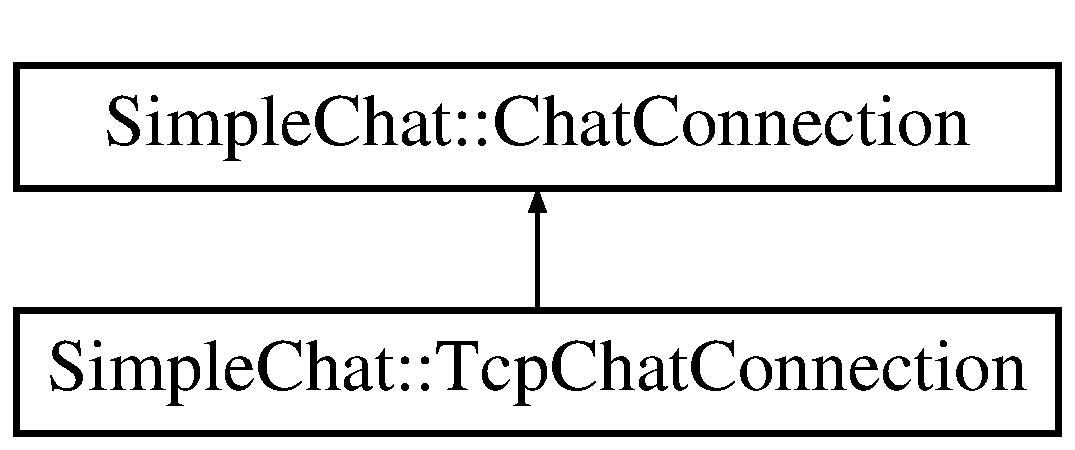
\includegraphics[height=2.000000cm]{classSimpleChat_1_1ChatConnection}
\end{center}
\end{figure}
\subsection*{Public Member Functions}
\begin{DoxyCompactItemize}
\item 
\hypertarget{classSimpleChat_1_1ChatConnection_af5672f1d6c37c218e777fb7622c349a1}{virtual bool {\bfseries send\-Message} (std\-::unique\-\_\-ptr$<$ \hyperlink{classSimpleChat_1_1AbstractMessage}{Abstract\-Message} $>$ message)=0}\label{classSimpleChat_1_1ChatConnection_af5672f1d6c37c218e777fb7622c349a1}

\item 
\hypertarget{classSimpleChat_1_1ChatConnection_aa9b5995be550f047cc626655774dd8d4}{virtual bool {\bfseries is\-Alive} () const =0}\label{classSimpleChat_1_1ChatConnection_aa9b5995be550f047cc626655774dd8d4}

\item 
\hypertarget{classSimpleChat_1_1ChatConnection_ae054c601d19454d04501d386b17c9d86}{virtual std\-::string {\bfseries get\-Ident} () const =0}\label{classSimpleChat_1_1ChatConnection_ae054c601d19454d04501d386b17c9d86}

\item 
\hypertarget{classSimpleChat_1_1ChatConnection_a814ba178e2fd884bb4ec8d5dc191257b}{virtual void {\bfseries disconnect\-From\-Host} ()=0}\label{classSimpleChat_1_1ChatConnection_a814ba178e2fd884bb4ec8d5dc191257b}

\item 
\hypertarget{classSimpleChat_1_1ChatConnection_aedb96479d631cfdcd4014a5e242aa302}{virtual void {\bfseries set\-Chatee} (const std\-::shared\-\_\-ptr$<$ \hyperlink{classSimpleChat_1_1Chatee}{Chatee} $>$ \&chatee)=0}\label{classSimpleChat_1_1ChatConnection_aedb96479d631cfdcd4014a5e242aa302}

\item 
\hypertarget{classSimpleChat_1_1ChatConnection_abe39f6641a66d0a440d66fca649a7357}{virtual std\-::shared\-\_\-ptr$<$ \hyperlink{classSimpleChat_1_1Chatee}{Chatee} $>$ {\bfseries chatee} () const =0}\label{classSimpleChat_1_1ChatConnection_abe39f6641a66d0a440d66fca649a7357}

\end{DoxyCompactItemize}


The documentation for this class was generated from the following file\-:\begin{DoxyCompactItemize}
\item 
chatlib/chat/Chat\-Connection.\-h\end{DoxyCompactItemize}

\hypertarget{classSimpleChat_1_1ChatDialog}{\section{Simple\-Chat\-:\-:Chat\-Dialog Class Reference}
\label{classSimpleChat_1_1ChatDialog}\index{Simple\-Chat\-::\-Chat\-Dialog@{Simple\-Chat\-::\-Chat\-Dialog}}
}
Inheritance diagram for Simple\-Chat\-:\-:Chat\-Dialog\-:\begin{figure}[H]
\begin{center}
\leavevmode
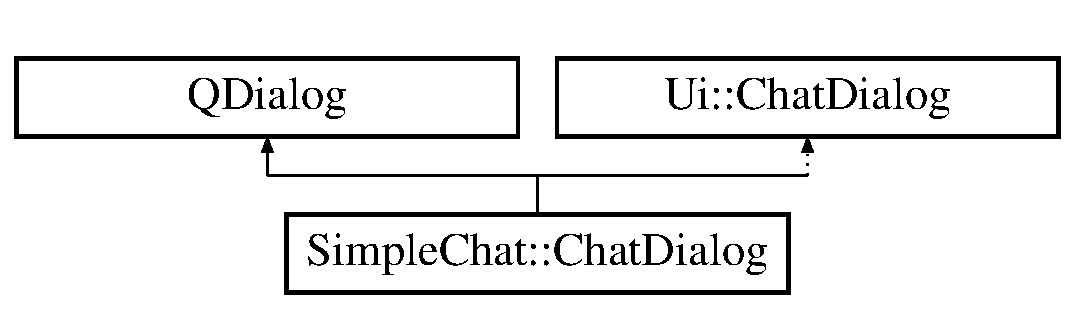
\includegraphics[height=2.000000cm]{classSimpleChat_1_1ChatDialog}
\end{center}
\end{figure}
\subsection*{Public Member Functions}
\begin{DoxyCompactItemize}
\item 
\hypertarget{classSimpleChat_1_1ChatDialog_a969efa56c5067874f46dca3d3eb0b84b}{{\bfseries Chat\-Dialog} (Q\-Widget $\ast$parent=nullptr)}\label{classSimpleChat_1_1ChatDialog_a969efa56c5067874f46dca3d3eb0b84b}

\item 
\hypertarget{classSimpleChat_1_1ChatDialog_ab20dcf9fbbbbfaa6f96adf505d3aaf7c}{void {\bfseries start} () const }\label{classSimpleChat_1_1ChatDialog_ab20dcf9fbbbbfaa6f96adf505d3aaf7c}

\end{DoxyCompactItemize}


The documentation for this class was generated from the following files\-:\begin{DoxyCompactItemize}
\item 
client/dialog/Chat\-Dialog.\-h\item 
client/dialog/Chat\-Dialog.\-cpp\end{DoxyCompactItemize}

\hypertarget{classUi_1_1ChatDialog}{\section{Ui\-:\-:Chat\-Dialog Class Reference}
\label{classUi_1_1ChatDialog}\index{Ui\-::\-Chat\-Dialog@{Ui\-::\-Chat\-Dialog}}
}
Inheritance diagram for Ui\-:\-:Chat\-Dialog\-:\begin{figure}[H]
\begin{center}
\leavevmode
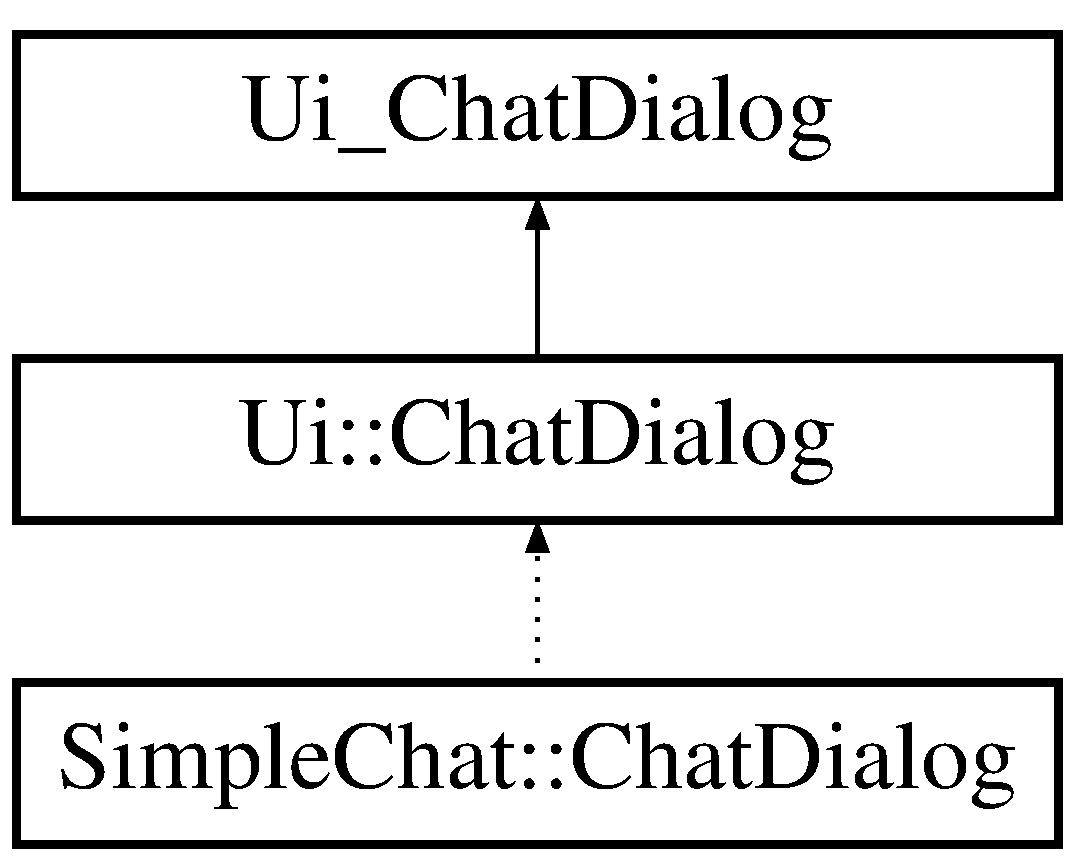
\includegraphics[height=3.000000cm]{classUi_1_1ChatDialog}
\end{center}
\end{figure}
\subsection*{Additional Inherited Members}


The documentation for this class was generated from the following file\-:\begin{DoxyCompactItemize}
\item 
client/ui\-\_\-chatdialog.\-h\end{DoxyCompactItemize}

\hypertarget{classSimpleChat_1_1Chatee}{\section{Simple\-Chat\-:\-:Chatee Class Reference}
\label{classSimpleChat_1_1Chatee}\index{Simple\-Chat\-::\-Chatee@{Simple\-Chat\-::\-Chatee}}
}
\subsection*{Public Member Functions}
\begin{DoxyCompactItemize}
\item 
\hypertarget{classSimpleChat_1_1Chatee_aa83e4ea06b6ff0ec85410c1abb2cc62b}{{\bfseries Chatee} (const \hyperlink{classSimpleChat_1_1User}{User} \&user, \hyperlink{classSimpleChat_1_1ChatConnection}{Chat\-Connection} $\ast$connection, std\-::shared\-\_\-ptr$<$ \hyperlink{classSimpleChat_1_1Chatroom}{Chatroom} $>$ chatroom)}\label{classSimpleChat_1_1Chatee_aa83e4ea06b6ff0ec85410c1abb2cc62b}

\item 
\hypertarget{classSimpleChat_1_1Chatee_a7fbd4397978d0c603a9a485ad78d60ba}{\hyperlink{classSimpleChat_1_1User}{User} \& {\bfseries user} ()}\label{classSimpleChat_1_1Chatee_a7fbd4397978d0c603a9a485ad78d60ba}

\item 
\hypertarget{classSimpleChat_1_1Chatee_a50dd83ccddcb599fc6a9ed0dfb7f5f1e}{bool {\bfseries send\-Message} (std\-::unique\-\_\-ptr$<$ \hyperlink{classSimpleChat_1_1AbstractMessage}{Abstract\-Message} $>$ message)}\label{classSimpleChat_1_1Chatee_a50dd83ccddcb599fc6a9ed0dfb7f5f1e}

\item 
\hypertarget{classSimpleChat_1_1Chatee_a4678783008a283355896b32643b881bc}{void {\bfseries send\-Chat\-Message} (const std\-::string \&message, const std\-::string \&from, const std\-::string \&target=\char`\"{}\char`\"{})}\label{classSimpleChat_1_1Chatee_a4678783008a283355896b32643b881bc}

\item 
\hypertarget{classSimpleChat_1_1Chatee_ab06c30e73c50b3f0daa55834fc160e96}{void {\bfseries send\-Response} (bool success, const std\-::string \&message)}\label{classSimpleChat_1_1Chatee_ab06c30e73c50b3f0daa55834fc160e96}

\item 
\hypertarget{classSimpleChat_1_1Chatee_afe41bc771c6ed37cb46e05d81e8f8167}{void {\bfseries mute} (bool propagate)}\label{classSimpleChat_1_1Chatee_afe41bc771c6ed37cb46e05d81e8f8167}

\item 
\hypertarget{classSimpleChat_1_1Chatee_a51783a98bb0247d3590ce8bb1ba4ab71}{void {\bfseries unmute} (bool propagate)}\label{classSimpleChat_1_1Chatee_a51783a98bb0247d3590ce8bb1ba4ab71}

\item 
void \hyperlink{classSimpleChat_1_1Chatee_a6f559b4a9199f412a1daeb601b935ac9}{kick} (bool propagate)
\item 
\hypertarget{classSimpleChat_1_1Chatee_ae12a6ade9ae6daca07608acc88d5cfc0}{\hyperlink{classSimpleChat_1_1ChatConnection}{Chat\-Connection} $\ast$ {\bfseries connection} () const }\label{classSimpleChat_1_1Chatee_ae12a6ade9ae6daca07608acc88d5cfc0}

\item 
\hypertarget{classSimpleChat_1_1Chatee_a8c22ba161574ce78241a1635ee214ee8}{bool {\bfseries authorized} () const }\label{classSimpleChat_1_1Chatee_a8c22ba161574ce78241a1635ee214ee8}

\item 
\hypertarget{classSimpleChat_1_1Chatee_a51edbd8720b88b68761c0ebcbd8cc4c0}{void {\bfseries set\-Authorized} (bool authorized)}\label{classSimpleChat_1_1Chatee_a51edbd8720b88b68761c0ebcbd8cc4c0}

\end{DoxyCompactItemize}


\subsection{Member Function Documentation}
\hypertarget{classSimpleChat_1_1Chatee_a6f559b4a9199f412a1daeb601b935ac9}{\index{Simple\-Chat\-::\-Chatee@{Simple\-Chat\-::\-Chatee}!kick@{kick}}
\index{kick@{kick}!SimpleChat::Chatee@{Simple\-Chat\-::\-Chatee}}
\subsubsection[{kick}]{\setlength{\rightskip}{0pt plus 5cm}void Simple\-Chat\-::\-Chatee\-::kick (
\begin{DoxyParamCaption}
\item[{bool}]{propagate}
\end{DoxyParamCaption}
)}}\label{classSimpleChat_1_1Chatee_a6f559b4a9199f412a1daeb601b935ac9}
propagate will be true when the server calls this function so we should drop the connection to the kicked client 

The documentation for this class was generated from the following files\-:\begin{DoxyCompactItemize}
\item 
chatlib/chat/Chatee.\-h\item 
chatlib/chat/Chatee.\-cpp\end{DoxyCompactItemize}

\hypertarget{classSimpleChat_1_1ChatMessage}{\section{Simple\-Chat\-:\-:Chat\-Message Class Reference}
\label{classSimpleChat_1_1ChatMessage}\index{Simple\-Chat\-::\-Chat\-Message@{Simple\-Chat\-::\-Chat\-Message}}
}
Inheritance diagram for Simple\-Chat\-:\-:Chat\-Message\-:\begin{figure}[H]
\begin{center}
\leavevmode
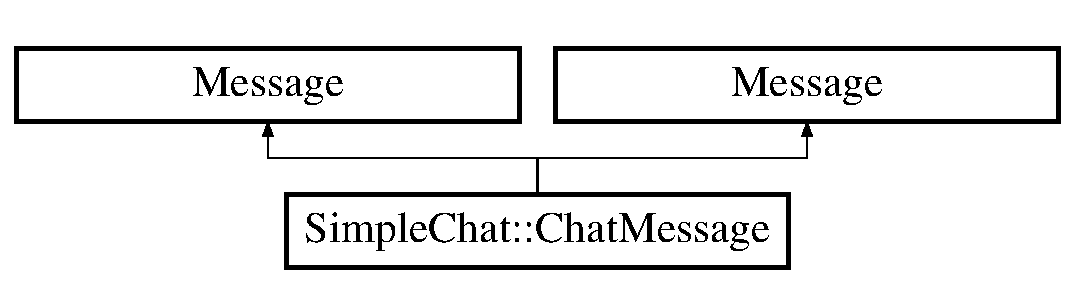
\includegraphics[height=2.000000cm]{classSimpleChat_1_1ChatMessage}
\end{center}
\end{figure}
\subsection*{Public Member Functions}
\begin{DoxyCompactItemize}
\item 
\hypertarget{classSimpleChat_1_1ChatMessage_a231f5e8f74e136753ca49ea5ca9ae51f}{{\bfseries Chat\-Message} (const \hyperlink{classSimpleChat_1_1ChatMessage}{Chat\-Message} \&from)}\label{classSimpleChat_1_1ChatMessage_a231f5e8f74e136753ca49ea5ca9ae51f}

\item 
\hypertarget{classSimpleChat_1_1ChatMessage_ade94e82145002b81dfa9e2f35855084f}{\hyperlink{classSimpleChat_1_1ChatMessage}{Chat\-Message} \& {\bfseries operator=} (const \hyperlink{classSimpleChat_1_1ChatMessage}{Chat\-Message} \&from)}\label{classSimpleChat_1_1ChatMessage_ade94e82145002b81dfa9e2f35855084f}

\item 
\hypertarget{classSimpleChat_1_1ChatMessage_a261d1bfeea73eb6eb16ecaf27d770be1}{const \\*
\-::google\-::protobuf\-::\-Unknown\-Field\-Set \& {\bfseries unknown\-\_\-fields} () const }\label{classSimpleChat_1_1ChatMessage_a261d1bfeea73eb6eb16ecaf27d770be1}

\item 
\hypertarget{classSimpleChat_1_1ChatMessage_a6ddd70adfef9a10e694f12350ae29382}{inline\-::google\-::protobuf\-::\-Unknown\-Field\-Set $\ast$ {\bfseries mutable\-\_\-unknown\-\_\-fields} ()}\label{classSimpleChat_1_1ChatMessage_a6ddd70adfef9a10e694f12350ae29382}

\item 
\hypertarget{classSimpleChat_1_1ChatMessage_a8d7cf0c94da9a697d77641dfd9a17310}{void {\bfseries Swap} (\hyperlink{classSimpleChat_1_1ChatMessage}{Chat\-Message} $\ast$other)}\label{classSimpleChat_1_1ChatMessage_a8d7cf0c94da9a697d77641dfd9a17310}

\item 
\hypertarget{classSimpleChat_1_1ChatMessage_a0837c7d0ab99ab83af09f4d695c5fa2b}{\hyperlink{classSimpleChat_1_1ChatMessage}{Chat\-Message} $\ast$ {\bfseries New} () const }\label{classSimpleChat_1_1ChatMessage_a0837c7d0ab99ab83af09f4d695c5fa2b}

\item 
\hypertarget{classSimpleChat_1_1ChatMessage_a8bfb7e74e37956c08734a8ad0e165746}{\hyperlink{classSimpleChat_1_1ChatMessage}{Chat\-Message} $\ast$ {\bfseries New} (\-::google\-::protobuf\-::\-Arena $\ast$arena) const }\label{classSimpleChat_1_1ChatMessage_a8bfb7e74e37956c08734a8ad0e165746}

\item 
\hypertarget{classSimpleChat_1_1ChatMessage_ab76ad9474fddf3fff5e8ac32baced6f9}{void {\bfseries Copy\-From} (const \-::google\-::protobuf\-::\-Message \&from)}\label{classSimpleChat_1_1ChatMessage_ab76ad9474fddf3fff5e8ac32baced6f9}

\item 
\hypertarget{classSimpleChat_1_1ChatMessage_a08b1dd53a5f0883e4b1c654d0d42c41f}{void {\bfseries Merge\-From} (const \-::google\-::protobuf\-::\-Message \&from)}\label{classSimpleChat_1_1ChatMessage_a08b1dd53a5f0883e4b1c654d0d42c41f}

\item 
\hypertarget{classSimpleChat_1_1ChatMessage_a9d0c6023de82cce729a4adfd0dab3fff}{void {\bfseries Copy\-From} (const \hyperlink{classSimpleChat_1_1ChatMessage}{Chat\-Message} \&from)}\label{classSimpleChat_1_1ChatMessage_a9d0c6023de82cce729a4adfd0dab3fff}

\item 
\hypertarget{classSimpleChat_1_1ChatMessage_a3ed1b027416e9e87e0cccfcc667eab28}{void {\bfseries Merge\-From} (const \hyperlink{classSimpleChat_1_1ChatMessage}{Chat\-Message} \&from)}\label{classSimpleChat_1_1ChatMessage_a3ed1b027416e9e87e0cccfcc667eab28}

\item 
\hypertarget{classSimpleChat_1_1ChatMessage_aa8568ebe3b5f1f0d8178db2838bce038}{void {\bfseries Clear} ()}\label{classSimpleChat_1_1ChatMessage_aa8568ebe3b5f1f0d8178db2838bce038}

\item 
\hypertarget{classSimpleChat_1_1ChatMessage_ab63f1149ba872d70d8eefcc85072bf0c}{bool {\bfseries Is\-Initialized} () const }\label{classSimpleChat_1_1ChatMessage_ab63f1149ba872d70d8eefcc85072bf0c}

\item 
\hypertarget{classSimpleChat_1_1ChatMessage_aa70f05d5b4548467d2568c8650c38691}{int {\bfseries Byte\-Size} () const }\label{classSimpleChat_1_1ChatMessage_aa70f05d5b4548467d2568c8650c38691}

\item 
\hypertarget{classSimpleChat_1_1ChatMessage_a2d550974195d6f5937eb465bea89844e}{bool {\bfseries Merge\-Partial\-From\-Coded\-Stream} (\-::google\-::protobuf\-::io\-::\-Coded\-Input\-Stream $\ast$input)}\label{classSimpleChat_1_1ChatMessage_a2d550974195d6f5937eb465bea89844e}

\item 
\hypertarget{classSimpleChat_1_1ChatMessage_a07a1a27d06b606f2171565d473a8d800}{void {\bfseries Serialize\-With\-Cached\-Sizes} (\-::google\-::protobuf\-::io\-::\-Coded\-Output\-Stream $\ast$output) const }\label{classSimpleChat_1_1ChatMessage_a07a1a27d06b606f2171565d473a8d800}

\item 
\hypertarget{classSimpleChat_1_1ChatMessage_ac4a70b6b83215b2b3316a5977b4358ed}{\-::google\-::protobuf\-::uint8 $\ast$ {\bfseries Serialize\-With\-Cached\-Sizes\-To\-Array} (\-::google\-::protobuf\-::uint8 $\ast$output) const }\label{classSimpleChat_1_1ChatMessage_ac4a70b6b83215b2b3316a5977b4358ed}

\item 
\hypertarget{classSimpleChat_1_1ChatMessage_a1215ab1d24366ed5bf9551577f21bbc1}{int {\bfseries Get\-Cached\-Size} () const }\label{classSimpleChat_1_1ChatMessage_a1215ab1d24366ed5bf9551577f21bbc1}

\item 
\hypertarget{classSimpleChat_1_1ChatMessage_a8e0c6d4861d69d78af5217d483fccd37}{\-::google\-::protobuf\-::\-Metadata {\bfseries Get\-Metadata} () const }\label{classSimpleChat_1_1ChatMessage_a8e0c6d4861d69d78af5217d483fccd37}

\item 
\hypertarget{classSimpleChat_1_1ChatMessage_a901fbde55bb58cc724872b5220251f56}{bool {\bfseries has\-\_\-text} () const }\label{classSimpleChat_1_1ChatMessage_a901fbde55bb58cc724872b5220251f56}

\item 
\hypertarget{classSimpleChat_1_1ChatMessage_a294a98242872e1c527bd7903b2e731a6}{void {\bfseries clear\-\_\-text} ()}\label{classSimpleChat_1_1ChatMessage_a294a98242872e1c527bd7903b2e731a6}

\item 
\hypertarget{classSimpleChat_1_1ChatMessage_ab0c72246a3151e5df8964a15867ed1cd}{const \-::std\-::string \& {\bfseries text} () const }\label{classSimpleChat_1_1ChatMessage_ab0c72246a3151e5df8964a15867ed1cd}

\item 
\hypertarget{classSimpleChat_1_1ChatMessage_ab2d1b74910a49a62af274335b16a7fd1}{void {\bfseries set\-\_\-text} (const \-::std\-::string \&value)}\label{classSimpleChat_1_1ChatMessage_ab2d1b74910a49a62af274335b16a7fd1}

\item 
\hypertarget{classSimpleChat_1_1ChatMessage_a6e3772b230734b792ffadf740fbdd0e8}{void {\bfseries set\-\_\-text} (const char $\ast$value)}\label{classSimpleChat_1_1ChatMessage_a6e3772b230734b792ffadf740fbdd0e8}

\item 
\hypertarget{classSimpleChat_1_1ChatMessage_abbfa9789b7cf6a91126081bed83ea4e8}{void {\bfseries set\-\_\-text} (const char $\ast$value, size\-\_\-t size)}\label{classSimpleChat_1_1ChatMessage_abbfa9789b7cf6a91126081bed83ea4e8}

\item 
\hypertarget{classSimpleChat_1_1ChatMessage_ab27d1c1071ce19816f6bb328a0c2c667}{\-::std\-::string $\ast$ {\bfseries mutable\-\_\-text} ()}\label{classSimpleChat_1_1ChatMessage_ab27d1c1071ce19816f6bb328a0c2c667}

\item 
\hypertarget{classSimpleChat_1_1ChatMessage_ab57c4fa5ee811a57f2ed261b6e4086a7}{\-::std\-::string $\ast$ {\bfseries release\-\_\-text} ()}\label{classSimpleChat_1_1ChatMessage_ab57c4fa5ee811a57f2ed261b6e4086a7}

\item 
\hypertarget{classSimpleChat_1_1ChatMessage_ae863497ba313a809ee4ce02dc40632f9}{void {\bfseries set\-\_\-allocated\-\_\-text} (\-::std\-::string $\ast$text)}\label{classSimpleChat_1_1ChatMessage_ae863497ba313a809ee4ce02dc40632f9}

\item 
\hypertarget{classSimpleChat_1_1ChatMessage_a4aceacb01a84a74b1cb9fb537d087461}{bool {\bfseries has\-\_\-from} () const }\label{classSimpleChat_1_1ChatMessage_a4aceacb01a84a74b1cb9fb537d087461}

\item 
\hypertarget{classSimpleChat_1_1ChatMessage_a280ea2eeb3c38b1921cdbd89dad08fdc}{void {\bfseries clear\-\_\-from} ()}\label{classSimpleChat_1_1ChatMessage_a280ea2eeb3c38b1921cdbd89dad08fdc}

\item 
\hypertarget{classSimpleChat_1_1ChatMessage_a64cab764c417f41d8c7856a45a97ee0c}{const \-::\hyperlink{classSimpleChat_1_1ChatTarget}{Simple\-Chat\-::\-Chat\-Target} \& {\bfseries from} () const }\label{classSimpleChat_1_1ChatMessage_a64cab764c417f41d8c7856a45a97ee0c}

\item 
\hypertarget{classSimpleChat_1_1ChatMessage_a17867bdc8208522f8dbe25f08beb37c2}{\-::\hyperlink{classSimpleChat_1_1ChatTarget}{Simple\-Chat\-::\-Chat\-Target} $\ast$ {\bfseries mutable\-\_\-from} ()}\label{classSimpleChat_1_1ChatMessage_a17867bdc8208522f8dbe25f08beb37c2}

\item 
\hypertarget{classSimpleChat_1_1ChatMessage_a98cfe09cbfa47ce5a3391e7b6b050c9d}{\-::\hyperlink{classSimpleChat_1_1ChatTarget}{Simple\-Chat\-::\-Chat\-Target} $\ast$ {\bfseries release\-\_\-from} ()}\label{classSimpleChat_1_1ChatMessage_a98cfe09cbfa47ce5a3391e7b6b050c9d}

\item 
\hypertarget{classSimpleChat_1_1ChatMessage_aecb81c970857879f6e8261d1cfb4ecaf}{void {\bfseries set\-\_\-allocated\-\_\-from} (\-::\hyperlink{classSimpleChat_1_1ChatTarget}{Simple\-Chat\-::\-Chat\-Target} $\ast$from)}\label{classSimpleChat_1_1ChatMessage_aecb81c970857879f6e8261d1cfb4ecaf}

\item 
\hypertarget{classSimpleChat_1_1ChatMessage_a704f255c6091ba78db772cf78fde0c29}{bool {\bfseries has\-\_\-target} () const }\label{classSimpleChat_1_1ChatMessage_a704f255c6091ba78db772cf78fde0c29}

\item 
\hypertarget{classSimpleChat_1_1ChatMessage_a144663c85b22b0f79a079c0c575ce96f}{void {\bfseries clear\-\_\-target} ()}\label{classSimpleChat_1_1ChatMessage_a144663c85b22b0f79a079c0c575ce96f}

\item 
\hypertarget{classSimpleChat_1_1ChatMessage_a78c3116e0523179d5118ad7779df428b}{const \-::\hyperlink{classSimpleChat_1_1ChatTarget}{Simple\-Chat\-::\-Chat\-Target} \& {\bfseries target} () const }\label{classSimpleChat_1_1ChatMessage_a78c3116e0523179d5118ad7779df428b}

\item 
\hypertarget{classSimpleChat_1_1ChatMessage_a0f912be120023583235c0c6ae7e0e660}{\-::\hyperlink{classSimpleChat_1_1ChatTarget}{Simple\-Chat\-::\-Chat\-Target} $\ast$ {\bfseries mutable\-\_\-target} ()}\label{classSimpleChat_1_1ChatMessage_a0f912be120023583235c0c6ae7e0e660}

\item 
\hypertarget{classSimpleChat_1_1ChatMessage_a5de53b4a708a5a58772c58f46c9c9bd2}{\-::\hyperlink{classSimpleChat_1_1ChatTarget}{Simple\-Chat\-::\-Chat\-Target} $\ast$ {\bfseries release\-\_\-target} ()}\label{classSimpleChat_1_1ChatMessage_a5de53b4a708a5a58772c58f46c9c9bd2}

\item 
\hypertarget{classSimpleChat_1_1ChatMessage_a7c2bfae57846308a1a553b70b558ce99}{void {\bfseries set\-\_\-allocated\-\_\-target} (\-::\hyperlink{classSimpleChat_1_1ChatTarget}{Simple\-Chat\-::\-Chat\-Target} $\ast$target)}\label{classSimpleChat_1_1ChatMessage_a7c2bfae57846308a1a553b70b558ce99}

\item 
\hypertarget{classSimpleChat_1_1ChatMessage_a231f5e8f74e136753ca49ea5ca9ae51f}{{\bfseries Chat\-Message} (const \hyperlink{classSimpleChat_1_1ChatMessage}{Chat\-Message} \&from)}\label{classSimpleChat_1_1ChatMessage_a231f5e8f74e136753ca49ea5ca9ae51f}

\item 
\hypertarget{classSimpleChat_1_1ChatMessage_ade94e82145002b81dfa9e2f35855084f}{\hyperlink{classSimpleChat_1_1ChatMessage}{Chat\-Message} \& {\bfseries operator=} (const \hyperlink{classSimpleChat_1_1ChatMessage}{Chat\-Message} \&from)}\label{classSimpleChat_1_1ChatMessage_ade94e82145002b81dfa9e2f35855084f}

\item 
\hypertarget{classSimpleChat_1_1ChatMessage_a261d1bfeea73eb6eb16ecaf27d770be1}{const \\*
\-::google\-::protobuf\-::\-Unknown\-Field\-Set \& {\bfseries unknown\-\_\-fields} () const }\label{classSimpleChat_1_1ChatMessage_a261d1bfeea73eb6eb16ecaf27d770be1}

\item 
\hypertarget{classSimpleChat_1_1ChatMessage_a6ddd70adfef9a10e694f12350ae29382}{inline\-::google\-::protobuf\-::\-Unknown\-Field\-Set $\ast$ {\bfseries mutable\-\_\-unknown\-\_\-fields} ()}\label{classSimpleChat_1_1ChatMessage_a6ddd70adfef9a10e694f12350ae29382}

\item 
\hypertarget{classSimpleChat_1_1ChatMessage_a8d7cf0c94da9a697d77641dfd9a17310}{void {\bfseries Swap} (\hyperlink{classSimpleChat_1_1ChatMessage}{Chat\-Message} $\ast$other)}\label{classSimpleChat_1_1ChatMessage_a8d7cf0c94da9a697d77641dfd9a17310}

\item 
\hypertarget{classSimpleChat_1_1ChatMessage_a0837c7d0ab99ab83af09f4d695c5fa2b}{\hyperlink{classSimpleChat_1_1ChatMessage}{Chat\-Message} $\ast$ {\bfseries New} () const }\label{classSimpleChat_1_1ChatMessage_a0837c7d0ab99ab83af09f4d695c5fa2b}

\item 
\hypertarget{classSimpleChat_1_1ChatMessage_a8bfb7e74e37956c08734a8ad0e165746}{\hyperlink{classSimpleChat_1_1ChatMessage}{Chat\-Message} $\ast$ {\bfseries New} (\-::google\-::protobuf\-::\-Arena $\ast$arena) const }\label{classSimpleChat_1_1ChatMessage_a8bfb7e74e37956c08734a8ad0e165746}

\item 
\hypertarget{classSimpleChat_1_1ChatMessage_ab76ad9474fddf3fff5e8ac32baced6f9}{void {\bfseries Copy\-From} (const \-::google\-::protobuf\-::\-Message \&from)}\label{classSimpleChat_1_1ChatMessage_ab76ad9474fddf3fff5e8ac32baced6f9}

\item 
\hypertarget{classSimpleChat_1_1ChatMessage_a08b1dd53a5f0883e4b1c654d0d42c41f}{void {\bfseries Merge\-From} (const \-::google\-::protobuf\-::\-Message \&from)}\label{classSimpleChat_1_1ChatMessage_a08b1dd53a5f0883e4b1c654d0d42c41f}

\item 
\hypertarget{classSimpleChat_1_1ChatMessage_a9d0c6023de82cce729a4adfd0dab3fff}{void {\bfseries Copy\-From} (const \hyperlink{classSimpleChat_1_1ChatMessage}{Chat\-Message} \&from)}\label{classSimpleChat_1_1ChatMessage_a9d0c6023de82cce729a4adfd0dab3fff}

\item 
\hypertarget{classSimpleChat_1_1ChatMessage_a3ed1b027416e9e87e0cccfcc667eab28}{void {\bfseries Merge\-From} (const \hyperlink{classSimpleChat_1_1ChatMessage}{Chat\-Message} \&from)}\label{classSimpleChat_1_1ChatMessage_a3ed1b027416e9e87e0cccfcc667eab28}

\item 
\hypertarget{classSimpleChat_1_1ChatMessage_aa8568ebe3b5f1f0d8178db2838bce038}{void {\bfseries Clear} ()}\label{classSimpleChat_1_1ChatMessage_aa8568ebe3b5f1f0d8178db2838bce038}

\item 
\hypertarget{classSimpleChat_1_1ChatMessage_ab63f1149ba872d70d8eefcc85072bf0c}{bool {\bfseries Is\-Initialized} () const }\label{classSimpleChat_1_1ChatMessage_ab63f1149ba872d70d8eefcc85072bf0c}

\item 
\hypertarget{classSimpleChat_1_1ChatMessage_aa70f05d5b4548467d2568c8650c38691}{int {\bfseries Byte\-Size} () const }\label{classSimpleChat_1_1ChatMessage_aa70f05d5b4548467d2568c8650c38691}

\item 
\hypertarget{classSimpleChat_1_1ChatMessage_a2d550974195d6f5937eb465bea89844e}{bool {\bfseries Merge\-Partial\-From\-Coded\-Stream} (\-::google\-::protobuf\-::io\-::\-Coded\-Input\-Stream $\ast$input)}\label{classSimpleChat_1_1ChatMessage_a2d550974195d6f5937eb465bea89844e}

\item 
\hypertarget{classSimpleChat_1_1ChatMessage_a07a1a27d06b606f2171565d473a8d800}{void {\bfseries Serialize\-With\-Cached\-Sizes} (\-::google\-::protobuf\-::io\-::\-Coded\-Output\-Stream $\ast$output) const }\label{classSimpleChat_1_1ChatMessage_a07a1a27d06b606f2171565d473a8d800}

\item 
\hypertarget{classSimpleChat_1_1ChatMessage_ac4a70b6b83215b2b3316a5977b4358ed}{\-::google\-::protobuf\-::uint8 $\ast$ {\bfseries Serialize\-With\-Cached\-Sizes\-To\-Array} (\-::google\-::protobuf\-::uint8 $\ast$output) const }\label{classSimpleChat_1_1ChatMessage_ac4a70b6b83215b2b3316a5977b4358ed}

\item 
\hypertarget{classSimpleChat_1_1ChatMessage_a1215ab1d24366ed5bf9551577f21bbc1}{int {\bfseries Get\-Cached\-Size} () const }\label{classSimpleChat_1_1ChatMessage_a1215ab1d24366ed5bf9551577f21bbc1}

\item 
\hypertarget{classSimpleChat_1_1ChatMessage_a8e0c6d4861d69d78af5217d483fccd37}{\-::google\-::protobuf\-::\-Metadata {\bfseries Get\-Metadata} () const }\label{classSimpleChat_1_1ChatMessage_a8e0c6d4861d69d78af5217d483fccd37}

\item 
\hypertarget{classSimpleChat_1_1ChatMessage_a901fbde55bb58cc724872b5220251f56}{bool {\bfseries has\-\_\-text} () const }\label{classSimpleChat_1_1ChatMessage_a901fbde55bb58cc724872b5220251f56}

\item 
\hypertarget{classSimpleChat_1_1ChatMessage_a294a98242872e1c527bd7903b2e731a6}{void {\bfseries clear\-\_\-text} ()}\label{classSimpleChat_1_1ChatMessage_a294a98242872e1c527bd7903b2e731a6}

\item 
\hypertarget{classSimpleChat_1_1ChatMessage_af76a34c44f4d36950b995a5fcab0934d}{const \-::std\-::string \& {\bfseries text} () const }\label{classSimpleChat_1_1ChatMessage_af76a34c44f4d36950b995a5fcab0934d}

\item 
\hypertarget{classSimpleChat_1_1ChatMessage_ab2d1b74910a49a62af274335b16a7fd1}{void {\bfseries set\-\_\-text} (const \-::std\-::string \&value)}\label{classSimpleChat_1_1ChatMessage_ab2d1b74910a49a62af274335b16a7fd1}

\item 
\hypertarget{classSimpleChat_1_1ChatMessage_a6e3772b230734b792ffadf740fbdd0e8}{void {\bfseries set\-\_\-text} (const char $\ast$value)}\label{classSimpleChat_1_1ChatMessage_a6e3772b230734b792ffadf740fbdd0e8}

\item 
\hypertarget{classSimpleChat_1_1ChatMessage_abbfa9789b7cf6a91126081bed83ea4e8}{void {\bfseries set\-\_\-text} (const char $\ast$value, size\-\_\-t size)}\label{classSimpleChat_1_1ChatMessage_abbfa9789b7cf6a91126081bed83ea4e8}

\item 
\hypertarget{classSimpleChat_1_1ChatMessage_a6a418cae3fc39d82b74cd86b31485072}{\-::std\-::string $\ast$ {\bfseries mutable\-\_\-text} ()}\label{classSimpleChat_1_1ChatMessage_a6a418cae3fc39d82b74cd86b31485072}

\item 
\hypertarget{classSimpleChat_1_1ChatMessage_a340f4dd1d9e617f2dee6a629f6d1e5e6}{\-::std\-::string $\ast$ {\bfseries release\-\_\-text} ()}\label{classSimpleChat_1_1ChatMessage_a340f4dd1d9e617f2dee6a629f6d1e5e6}

\item 
\hypertarget{classSimpleChat_1_1ChatMessage_ae863497ba313a809ee4ce02dc40632f9}{void {\bfseries set\-\_\-allocated\-\_\-text} (\-::std\-::string $\ast$text)}\label{classSimpleChat_1_1ChatMessage_ae863497ba313a809ee4ce02dc40632f9}

\item 
\hypertarget{classSimpleChat_1_1ChatMessage_a5b6e77d14c619e40abcda0c94ff7549c}{bool {\bfseries has\-\_\-timestamp} () const }\label{classSimpleChat_1_1ChatMessage_a5b6e77d14c619e40abcda0c94ff7549c}

\item 
\hypertarget{classSimpleChat_1_1ChatMessage_a89b59db69601462b2676f340d4669929}{void {\bfseries clear\-\_\-timestamp} ()}\label{classSimpleChat_1_1ChatMessage_a89b59db69601462b2676f340d4669929}

\item 
\hypertarget{classSimpleChat_1_1ChatMessage_ab4ccafc85d0a4d737093cf1ad3e86296}{\-::google\-::protobuf\-::int64 {\bfseries timestamp} () const }\label{classSimpleChat_1_1ChatMessage_ab4ccafc85d0a4d737093cf1ad3e86296}

\item 
\hypertarget{classSimpleChat_1_1ChatMessage_afaa7b4063a4687aa3ed8a678e9628292}{void {\bfseries set\-\_\-timestamp} (\-::google\-::protobuf\-::int64 value)}\label{classSimpleChat_1_1ChatMessage_afaa7b4063a4687aa3ed8a678e9628292}

\item 
\hypertarget{classSimpleChat_1_1ChatMessage_a4aceacb01a84a74b1cb9fb537d087461}{bool {\bfseries has\-\_\-from} () const }\label{classSimpleChat_1_1ChatMessage_a4aceacb01a84a74b1cb9fb537d087461}

\item 
\hypertarget{classSimpleChat_1_1ChatMessage_a280ea2eeb3c38b1921cdbd89dad08fdc}{void {\bfseries clear\-\_\-from} ()}\label{classSimpleChat_1_1ChatMessage_a280ea2eeb3c38b1921cdbd89dad08fdc}

\item 
\hypertarget{classSimpleChat_1_1ChatMessage_a9c9024d51c198a1c8c9c6352e0b05506}{const \-::\hyperlink{classSimpleChat_1_1ChatTarget}{Simple\-Chat\-::\-Chat\-Target} \& {\bfseries from} () const }\label{classSimpleChat_1_1ChatMessage_a9c9024d51c198a1c8c9c6352e0b05506}

\item 
\hypertarget{classSimpleChat_1_1ChatMessage_a5e0d272517a1890e303962b0032e2a23}{\-::\hyperlink{classSimpleChat_1_1ChatTarget}{Simple\-Chat\-::\-Chat\-Target} $\ast$ {\bfseries mutable\-\_\-from} ()}\label{classSimpleChat_1_1ChatMessage_a5e0d272517a1890e303962b0032e2a23}

\item 
\hypertarget{classSimpleChat_1_1ChatMessage_a02e230b7915b7ea84e2079147f6f4eec}{\-::\hyperlink{classSimpleChat_1_1ChatTarget}{Simple\-Chat\-::\-Chat\-Target} $\ast$ {\bfseries release\-\_\-from} ()}\label{classSimpleChat_1_1ChatMessage_a02e230b7915b7ea84e2079147f6f4eec}

\item 
\hypertarget{classSimpleChat_1_1ChatMessage_aecb81c970857879f6e8261d1cfb4ecaf}{void {\bfseries set\-\_\-allocated\-\_\-from} (\-::\hyperlink{classSimpleChat_1_1ChatTarget}{Simple\-Chat\-::\-Chat\-Target} $\ast$from)}\label{classSimpleChat_1_1ChatMessage_aecb81c970857879f6e8261d1cfb4ecaf}

\item 
\hypertarget{classSimpleChat_1_1ChatMessage_a704f255c6091ba78db772cf78fde0c29}{bool {\bfseries has\-\_\-target} () const }\label{classSimpleChat_1_1ChatMessage_a704f255c6091ba78db772cf78fde0c29}

\item 
\hypertarget{classSimpleChat_1_1ChatMessage_a144663c85b22b0f79a079c0c575ce96f}{void {\bfseries clear\-\_\-target} ()}\label{classSimpleChat_1_1ChatMessage_a144663c85b22b0f79a079c0c575ce96f}

\item 
\hypertarget{classSimpleChat_1_1ChatMessage_ae3d85472b51805a691e2356b7955a46d}{const \-::\hyperlink{classSimpleChat_1_1ChatTarget}{Simple\-Chat\-::\-Chat\-Target} \& {\bfseries target} () const }\label{classSimpleChat_1_1ChatMessage_ae3d85472b51805a691e2356b7955a46d}

\item 
\hypertarget{classSimpleChat_1_1ChatMessage_a626e31c4eef74b9166d0e848ab4fa74e}{\-::\hyperlink{classSimpleChat_1_1ChatTarget}{Simple\-Chat\-::\-Chat\-Target} $\ast$ {\bfseries mutable\-\_\-target} ()}\label{classSimpleChat_1_1ChatMessage_a626e31c4eef74b9166d0e848ab4fa74e}

\item 
\hypertarget{classSimpleChat_1_1ChatMessage_abf2b496e1ea68299c1064d2ac6704c09}{\-::\hyperlink{classSimpleChat_1_1ChatTarget}{Simple\-Chat\-::\-Chat\-Target} $\ast$ {\bfseries release\-\_\-target} ()}\label{classSimpleChat_1_1ChatMessage_abf2b496e1ea68299c1064d2ac6704c09}

\item 
\hypertarget{classSimpleChat_1_1ChatMessage_a7c2bfae57846308a1a553b70b558ce99}{void {\bfseries set\-\_\-allocated\-\_\-target} (\-::\hyperlink{classSimpleChat_1_1ChatTarget}{Simple\-Chat\-::\-Chat\-Target} $\ast$target)}\label{classSimpleChat_1_1ChatMessage_a7c2bfae57846308a1a553b70b558ce99}

\end{DoxyCompactItemize}
\subsection*{Static Public Member Functions}
\begin{DoxyCompactItemize}
\item 
\hypertarget{classSimpleChat_1_1ChatMessage_aaa3e96d79676a6db090ef3673c3d83bc}{static const \\*
\-::google\-::protobuf\-::\-Descriptor $\ast$ {\bfseries descriptor} ()}\label{classSimpleChat_1_1ChatMessage_aaa3e96d79676a6db090ef3673c3d83bc}

\item 
\hypertarget{classSimpleChat_1_1ChatMessage_a4d48b780815d1f79fc0d842328d517a9}{static const \hyperlink{classSimpleChat_1_1ChatMessage}{Chat\-Message} \& {\bfseries default\-\_\-instance} ()}\label{classSimpleChat_1_1ChatMessage_a4d48b780815d1f79fc0d842328d517a9}

\item 
\hypertarget{classSimpleChat_1_1ChatMessage_aaa3e96d79676a6db090ef3673c3d83bc}{static const \\*
\-::google\-::protobuf\-::\-Descriptor $\ast$ {\bfseries descriptor} ()}\label{classSimpleChat_1_1ChatMessage_aaa3e96d79676a6db090ef3673c3d83bc}

\item 
\hypertarget{classSimpleChat_1_1ChatMessage_a4d48b780815d1f79fc0d842328d517a9}{static const \hyperlink{classSimpleChat_1_1ChatMessage}{Chat\-Message} \& {\bfseries default\-\_\-instance} ()}\label{classSimpleChat_1_1ChatMessage_a4d48b780815d1f79fc0d842328d517a9}

\end{DoxyCompactItemize}
\subsection*{Static Public Attributes}
\begin{DoxyCompactItemize}
\item 
\hypertarget{classSimpleChat_1_1ChatMessage_a8f3988baed7f92a2d06dc68470bd9e83}{static const int {\bfseries k\-Text\-Field\-Number} = 1}\label{classSimpleChat_1_1ChatMessage_a8f3988baed7f92a2d06dc68470bd9e83}

\item 
\hypertarget{classSimpleChat_1_1ChatMessage_a0fbedada5a581810caed105b45f54a06}{static const int {\bfseries k\-From\-Field\-Number} = 2}\label{classSimpleChat_1_1ChatMessage_a0fbedada5a581810caed105b45f54a06}

\item 
\hypertarget{classSimpleChat_1_1ChatMessage_add4726728179ad57b2eeac2b0fc9a516}{static const int {\bfseries k\-Target\-Field\-Number} = 3}\label{classSimpleChat_1_1ChatMessage_add4726728179ad57b2eeac2b0fc9a516}

\item 
\hypertarget{classSimpleChat_1_1ChatMessage_a3762bdd14c1f6ce170c837f5a2d4e5d9}{static const int {\bfseries k\-Timestamp\-Field\-Number} = 2}\label{classSimpleChat_1_1ChatMessage_a3762bdd14c1f6ce170c837f5a2d4e5d9}

\end{DoxyCompactItemize}
\subsection*{Friends}
\begin{DoxyCompactItemize}
\item 
\hypertarget{classSimpleChat_1_1ChatMessage_ab0d9593aa41361f04ab91f917ef9ec0e}{void {\bfseries protobuf\-\_\-\-Add\-Desc\-\_\-\-Chat\-Message\-\_\-2eproto} ()}\label{classSimpleChat_1_1ChatMessage_ab0d9593aa41361f04ab91f917ef9ec0e}

\item 
\hypertarget{classSimpleChat_1_1ChatMessage_a4ca7b2c64786782406ca69f6ba39ccb2}{void {\bfseries protobuf\-\_\-\-Assign\-Desc\-\_\-\-Chat\-Message\-\_\-2eproto} ()}\label{classSimpleChat_1_1ChatMessage_a4ca7b2c64786782406ca69f6ba39ccb2}

\item 
\hypertarget{classSimpleChat_1_1ChatMessage_a78726b79d52a130a50d7670a5c0238fc}{void {\bfseries protobuf\-\_\-\-Shutdown\-File\-\_\-\-Chat\-Message\-\_\-2eproto} ()}\label{classSimpleChat_1_1ChatMessage_a78726b79d52a130a50d7670a5c0238fc}

\item 
\hypertarget{classSimpleChat_1_1ChatMessage_ab0d9593aa41361f04ab91f917ef9ec0e}{void {\bfseries protobuf\-\_\-\-Add\-Desc\-\_\-\-Chat\-Message\-\_\-2eproto} ()}\label{classSimpleChat_1_1ChatMessage_ab0d9593aa41361f04ab91f917ef9ec0e}

\item 
\hypertarget{classSimpleChat_1_1ChatMessage_a4ca7b2c64786782406ca69f6ba39ccb2}{void {\bfseries protobuf\-\_\-\-Assign\-Desc\-\_\-\-Chat\-Message\-\_\-2eproto} ()}\label{classSimpleChat_1_1ChatMessage_a4ca7b2c64786782406ca69f6ba39ccb2}

\item 
\hypertarget{classSimpleChat_1_1ChatMessage_a78726b79d52a130a50d7670a5c0238fc}{void {\bfseries protobuf\-\_\-\-Shutdown\-File\-\_\-\-Chat\-Message\-\_\-2eproto} ()}\label{classSimpleChat_1_1ChatMessage_a78726b79d52a130a50d7670a5c0238fc}

\end{DoxyCompactItemize}


The documentation for this class was generated from the following file\-:\begin{DoxyCompactItemize}
\item 
chatlib/proto/Chat\-Message.\-pb.\-h\end{DoxyCompactItemize}

\hypertarget{classSimpleChat_1_1Chatroom}{\section{Simple\-Chat\-:\-:Chatroom Class Reference}
\label{classSimpleChat_1_1Chatroom}\index{Simple\-Chat\-::\-Chatroom@{Simple\-Chat\-::\-Chatroom}}
}
Inheritance diagram for Simple\-Chat\-:\-:Chatroom\-:\begin{figure}[H]
\begin{center}
\leavevmode
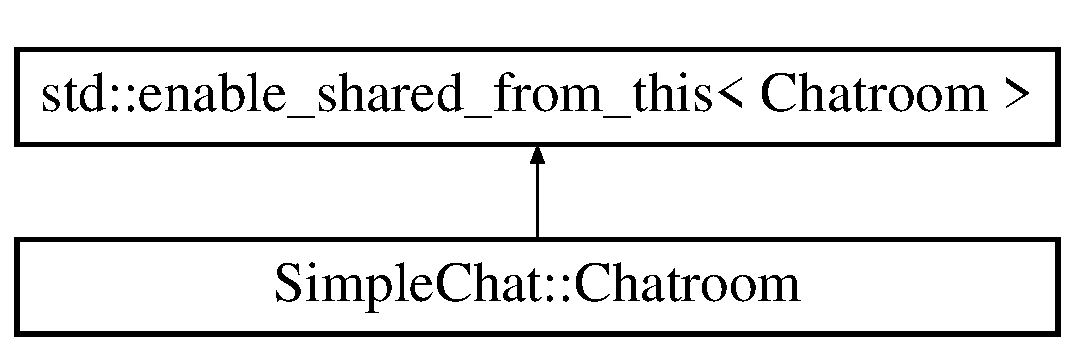
\includegraphics[height=2.000000cm]{classSimpleChat_1_1Chatroom}
\end{center}
\end{figure}
\subsection*{Public Member Functions}
\begin{DoxyCompactItemize}
\item 
\hypertarget{classSimpleChat_1_1Chatroom_abc9ca0382abb99ffd24860e8e32b5e3e}{std\-::tuple$<$ bool, std\-::string, \\*
std\-::shared\-\_\-ptr$<$ \hyperlink{classSimpleChat_1_1Chatee}{Chatee} $>$ $>$ {\bfseries chatee\-Joined} (const std\-::string \&name, \hyperlink{classSimpleChat_1_1ChatConnection}{Chat\-Connection} $\ast$connection)}\label{classSimpleChat_1_1Chatroom_abc9ca0382abb99ffd24860e8e32b5e3e}

\item 
\hypertarget{classSimpleChat_1_1Chatroom_a99f4d75b62c04d28f8da815a8fff46e0}{std\-::tuple$<$ bool, std\-::string, \\*
std\-::shared\-\_\-ptr$<$ \hyperlink{classSimpleChat_1_1Chatee}{Chatee} $>$ $>$ {\bfseries chatee\-Joined} (const \hyperlink{classSimpleChat_1_1User}{User} \&user, \hyperlink{classSimpleChat_1_1ChatConnection}{Chat\-Connection} $\ast$connection)}\label{classSimpleChat_1_1Chatroom_a99f4d75b62c04d28f8da815a8fff46e0}

\item 
\hypertarget{classSimpleChat_1_1Chatroom_a279a6c40a420063585609ebf6ed798e9}{std\-::tuple$<$ bool, std\-::string $>$ {\bfseries chatee\-Left} (const std\-::string \&name)}\label{classSimpleChat_1_1Chatroom_a279a6c40a420063585609ebf6ed798e9}

\item 
\hypertarget{classSimpleChat_1_1Chatroom_a79f00ddf84c6036bf4d327b1c2a552fa}{std\-::tuple$<$ bool, std\-::string $>$ {\bfseries chatee\-Left} (const \hyperlink{classSimpleChat_1_1User}{User} \&user)}\label{classSimpleChat_1_1Chatroom_a79f00ddf84c6036bf4d327b1c2a552fa}

\item 
\hypertarget{classSimpleChat_1_1Chatroom_a11d5b07b4e10b6e217b669756ecd936e}{void {\bfseries propagate\-Message} (std\-::unique\-\_\-ptr$<$ \hyperlink{classSimpleChat_1_1AbstractMessage}{Abstract\-Message} $>$ abstract\-Message) const }\label{classSimpleChat_1_1Chatroom_a11d5b07b4e10b6e217b669756ecd936e}

\item 
\hypertarget{classSimpleChat_1_1Chatroom_a78aae1327ee5cdc9010c707ca9f231c7}{bool {\bfseries chatee\-Exists} (const std\-::string \&name)}\label{classSimpleChat_1_1Chatroom_a78aae1327ee5cdc9010c707ca9f231c7}

\item 
\hypertarget{classSimpleChat_1_1Chatroom_a9c62326ce13b8406d6bc2e3aed7e2fd6}{std\-::shared\-\_\-ptr$<$ \hyperlink{classSimpleChat_1_1Chatee}{Chatee} $>$ {\bfseries get\-Chatee} (const std\-::string \&name)}\label{classSimpleChat_1_1Chatroom_a9c62326ce13b8406d6bc2e3aed7e2fd6}

\item 
\hypertarget{classSimpleChat_1_1Chatroom_ab6fdbdb57658dc86adfd5cf3917f25b0}{std\-::unique\-\_\-ptr$<$ \hyperlink{classSimpleChat_1_1ChatTarget}{Chat\-Target} $>$ {\bfseries get\-Target} (const std\-::string \&user\-Name)}\label{classSimpleChat_1_1Chatroom_ab6fdbdb57658dc86adfd5cf3917f25b0}

\item 
\hypertarget{classSimpleChat_1_1Chatroom_a551e00f5e376b0e8b158ba4fed5385b6}{void {\bfseries set\-Motd} (const std\-::string \&motd)}\label{classSimpleChat_1_1Chatroom_a551e00f5e376b0e8b158ba4fed5385b6}

\item 
\hypertarget{classSimpleChat_1_1Chatroom_a35c8905dbcc8f9426afe23266f9ea573}{std\-::string {\bfseries motd} ()}\label{classSimpleChat_1_1Chatroom_a35c8905dbcc8f9426afe23266f9ea573}

\item 
\hypertarget{classSimpleChat_1_1Chatroom_a32993b493fa3e141f5cae6ef757fd53e}{const Chatees\-Map \& {\bfseries map} () const }\label{classSimpleChat_1_1Chatroom_a32993b493fa3e141f5cae6ef757fd53e}

\end{DoxyCompactItemize}


The documentation for this class was generated from the following files\-:\begin{DoxyCompactItemize}
\item 
chatlib/chat/Chatroom.\-h\item 
chatlib/chat/Chatroom.\-cpp\end{DoxyCompactItemize}

\hypertarget{classSimpleChat_1_1ChatroomChange}{\section{Simple\-Chat\-:\-:Chatroom\-Change Class Reference}
\label{classSimpleChat_1_1ChatroomChange}\index{Simple\-Chat\-::\-Chatroom\-Change@{Simple\-Chat\-::\-Chatroom\-Change}}
}
Inheritance diagram for Simple\-Chat\-:\-:Chatroom\-Change\-:\begin{figure}[H]
\begin{center}
\leavevmode
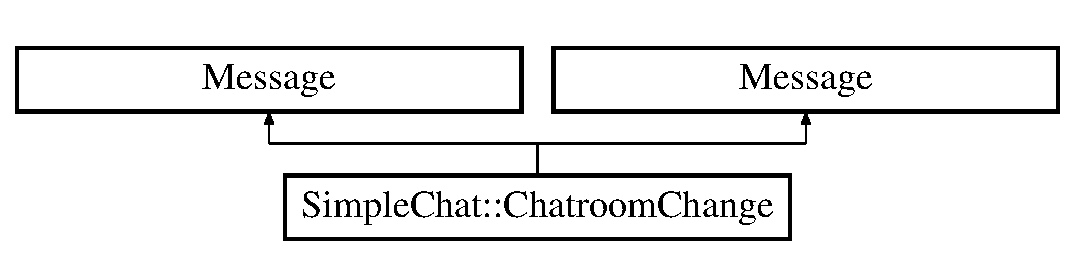
\includegraphics[height=2.000000cm]{classSimpleChat_1_1ChatroomChange}
\end{center}
\end{figure}
\subsection*{Public Member Functions}
\begin{DoxyCompactItemize}
\item 
\hypertarget{classSimpleChat_1_1ChatroomChange_abaead93fefe14aa4111dd7e40522ebc9}{{\bfseries Chatroom\-Change} (const \hyperlink{classSimpleChat_1_1ChatroomChange}{Chatroom\-Change} \&from)}\label{classSimpleChat_1_1ChatroomChange_abaead93fefe14aa4111dd7e40522ebc9}

\item 
\hypertarget{classSimpleChat_1_1ChatroomChange_a72f31bff580a7c9362661e5e77ac08ae}{\hyperlink{classSimpleChat_1_1ChatroomChange}{Chatroom\-Change} \& {\bfseries operator=} (const \hyperlink{classSimpleChat_1_1ChatroomChange}{Chatroom\-Change} \&from)}\label{classSimpleChat_1_1ChatroomChange_a72f31bff580a7c9362661e5e77ac08ae}

\item 
\hypertarget{classSimpleChat_1_1ChatroomChange_a0b223a07f61c3e24f31f342e4dd3cba2}{const \\*
\-::google\-::protobuf\-::\-Unknown\-Field\-Set \& {\bfseries unknown\-\_\-fields} () const }\label{classSimpleChat_1_1ChatroomChange_a0b223a07f61c3e24f31f342e4dd3cba2}

\item 
\hypertarget{classSimpleChat_1_1ChatroomChange_a3cd1b332a7d48c4e581efe06596edcb3}{inline\-::google\-::protobuf\-::\-Unknown\-Field\-Set $\ast$ {\bfseries mutable\-\_\-unknown\-\_\-fields} ()}\label{classSimpleChat_1_1ChatroomChange_a3cd1b332a7d48c4e581efe06596edcb3}

\item 
\hypertarget{classSimpleChat_1_1ChatroomChange_a43851d7c9b49cf1e9e9baccba6530b62}{void {\bfseries Swap} (\hyperlink{classSimpleChat_1_1ChatroomChange}{Chatroom\-Change} $\ast$other)}\label{classSimpleChat_1_1ChatroomChange_a43851d7c9b49cf1e9e9baccba6530b62}

\item 
\hypertarget{classSimpleChat_1_1ChatroomChange_adca2bbe6df3f78f3f1235097a7ca9a0b}{\hyperlink{classSimpleChat_1_1ChatroomChange}{Chatroom\-Change} $\ast$ {\bfseries New} () const }\label{classSimpleChat_1_1ChatroomChange_adca2bbe6df3f78f3f1235097a7ca9a0b}

\item 
\hypertarget{classSimpleChat_1_1ChatroomChange_a9de04796e81366af508d61df261b4d6b}{\hyperlink{classSimpleChat_1_1ChatroomChange}{Chatroom\-Change} $\ast$ {\bfseries New} (\-::google\-::protobuf\-::\-Arena $\ast$arena) const }\label{classSimpleChat_1_1ChatroomChange_a9de04796e81366af508d61df261b4d6b}

\item 
\hypertarget{classSimpleChat_1_1ChatroomChange_ac68b686d1309f3ecd6692c191cb854a9}{void {\bfseries Copy\-From} (const \-::google\-::protobuf\-::\-Message \&from)}\label{classSimpleChat_1_1ChatroomChange_ac68b686d1309f3ecd6692c191cb854a9}

\item 
\hypertarget{classSimpleChat_1_1ChatroomChange_aaf17b68dba7ef7f181c9bb217b822887}{void {\bfseries Merge\-From} (const \-::google\-::protobuf\-::\-Message \&from)}\label{classSimpleChat_1_1ChatroomChange_aaf17b68dba7ef7f181c9bb217b822887}

\item 
\hypertarget{classSimpleChat_1_1ChatroomChange_afb801d7bf6377b7c156a62e229f71c5c}{void {\bfseries Copy\-From} (const \hyperlink{classSimpleChat_1_1ChatroomChange}{Chatroom\-Change} \&from)}\label{classSimpleChat_1_1ChatroomChange_afb801d7bf6377b7c156a62e229f71c5c}

\item 
\hypertarget{classSimpleChat_1_1ChatroomChange_a2a314c25282ce98c6e35061a9251107d}{void {\bfseries Merge\-From} (const \hyperlink{classSimpleChat_1_1ChatroomChange}{Chatroom\-Change} \&from)}\label{classSimpleChat_1_1ChatroomChange_a2a314c25282ce98c6e35061a9251107d}

\item 
\hypertarget{classSimpleChat_1_1ChatroomChange_a15422c7efe2e8d9b9ec4782912b53871}{void {\bfseries Clear} ()}\label{classSimpleChat_1_1ChatroomChange_a15422c7efe2e8d9b9ec4782912b53871}

\item 
\hypertarget{classSimpleChat_1_1ChatroomChange_a0ccbfbeaa74853086743b47c9e51e0bb}{bool {\bfseries Is\-Initialized} () const }\label{classSimpleChat_1_1ChatroomChange_a0ccbfbeaa74853086743b47c9e51e0bb}

\item 
\hypertarget{classSimpleChat_1_1ChatroomChange_afb166debf92f4dfaeb0d65f6fdd8072b}{int {\bfseries Byte\-Size} () const }\label{classSimpleChat_1_1ChatroomChange_afb166debf92f4dfaeb0d65f6fdd8072b}

\item 
\hypertarget{classSimpleChat_1_1ChatroomChange_aa9437c9c14d96c00433739014292dbd6}{bool {\bfseries Merge\-Partial\-From\-Coded\-Stream} (\-::google\-::protobuf\-::io\-::\-Coded\-Input\-Stream $\ast$input)}\label{classSimpleChat_1_1ChatroomChange_aa9437c9c14d96c00433739014292dbd6}

\item 
\hypertarget{classSimpleChat_1_1ChatroomChange_ab401eaeaae01c66c4792748817cfbc5b}{void {\bfseries Serialize\-With\-Cached\-Sizes} (\-::google\-::protobuf\-::io\-::\-Coded\-Output\-Stream $\ast$output) const }\label{classSimpleChat_1_1ChatroomChange_ab401eaeaae01c66c4792748817cfbc5b}

\item 
\hypertarget{classSimpleChat_1_1ChatroomChange_af517a0d9b374b6c1ea5590c04d4903b1}{\-::google\-::protobuf\-::uint8 $\ast$ {\bfseries Serialize\-With\-Cached\-Sizes\-To\-Array} (\-::google\-::protobuf\-::uint8 $\ast$output) const }\label{classSimpleChat_1_1ChatroomChange_af517a0d9b374b6c1ea5590c04d4903b1}

\item 
\hypertarget{classSimpleChat_1_1ChatroomChange_a9cfe098f8c073092260a1b0e3c6faf0b}{int {\bfseries Get\-Cached\-Size} () const }\label{classSimpleChat_1_1ChatroomChange_a9cfe098f8c073092260a1b0e3c6faf0b}

\item 
\hypertarget{classSimpleChat_1_1ChatroomChange_ac6866dca8930acff0d42cb9f5e5c72dd}{\-::google\-::protobuf\-::\-Metadata {\bfseries Get\-Metadata} () const }\label{classSimpleChat_1_1ChatroomChange_ac6866dca8930acff0d42cb9f5e5c72dd}

\item 
\hypertarget{classSimpleChat_1_1ChatroomChange_aff68232dec1990b23c7e190104609a3c}{bool {\bfseries has\-\_\-motd} () const }\label{classSimpleChat_1_1ChatroomChange_aff68232dec1990b23c7e190104609a3c}

\item 
\hypertarget{classSimpleChat_1_1ChatroomChange_a4638d80e7cf3a6d547f3f588693fc7d3}{void {\bfseries clear\-\_\-motd} ()}\label{classSimpleChat_1_1ChatroomChange_a4638d80e7cf3a6d547f3f588693fc7d3}

\item 
\hypertarget{classSimpleChat_1_1ChatroomChange_a0e3dbc3b81fb01dca32b27f58b852e35}{const \-::std\-::string \& {\bfseries motd} () const }\label{classSimpleChat_1_1ChatroomChange_a0e3dbc3b81fb01dca32b27f58b852e35}

\item 
\hypertarget{classSimpleChat_1_1ChatroomChange_a0fa751b3f1896a808c15d52981fce7f2}{void {\bfseries set\-\_\-motd} (const \-::std\-::string \&value)}\label{classSimpleChat_1_1ChatroomChange_a0fa751b3f1896a808c15d52981fce7f2}

\item 
\hypertarget{classSimpleChat_1_1ChatroomChange_a2beea876aed1719e51735306647a9c8c}{void {\bfseries set\-\_\-motd} (const char $\ast$value)}\label{classSimpleChat_1_1ChatroomChange_a2beea876aed1719e51735306647a9c8c}

\item 
\hypertarget{classSimpleChat_1_1ChatroomChange_a302b59eb82dec05f2c24041632b85d57}{void {\bfseries set\-\_\-motd} (const char $\ast$value, size\-\_\-t size)}\label{classSimpleChat_1_1ChatroomChange_a302b59eb82dec05f2c24041632b85d57}

\item 
\hypertarget{classSimpleChat_1_1ChatroomChange_a82909be4fb8f30f192b623d0df979799}{\-::std\-::string $\ast$ {\bfseries mutable\-\_\-motd} ()}\label{classSimpleChat_1_1ChatroomChange_a82909be4fb8f30f192b623d0df979799}

\item 
\hypertarget{classSimpleChat_1_1ChatroomChange_a378806ad7c21608d4e349cf3c2ab256f}{\-::std\-::string $\ast$ {\bfseries release\-\_\-motd} ()}\label{classSimpleChat_1_1ChatroomChange_a378806ad7c21608d4e349cf3c2ab256f}

\item 
\hypertarget{classSimpleChat_1_1ChatroomChange_a8241c48fb8cfc701baeb0545bc4701b2}{void {\bfseries set\-\_\-allocated\-\_\-motd} (\-::std\-::string $\ast$motd)}\label{classSimpleChat_1_1ChatroomChange_a8241c48fb8cfc701baeb0545bc4701b2}

\item 
\hypertarget{classSimpleChat_1_1ChatroomChange_abaead93fefe14aa4111dd7e40522ebc9}{{\bfseries Chatroom\-Change} (const \hyperlink{classSimpleChat_1_1ChatroomChange}{Chatroom\-Change} \&from)}\label{classSimpleChat_1_1ChatroomChange_abaead93fefe14aa4111dd7e40522ebc9}

\item 
\hypertarget{classSimpleChat_1_1ChatroomChange_a72f31bff580a7c9362661e5e77ac08ae}{\hyperlink{classSimpleChat_1_1ChatroomChange}{Chatroom\-Change} \& {\bfseries operator=} (const \hyperlink{classSimpleChat_1_1ChatroomChange}{Chatroom\-Change} \&from)}\label{classSimpleChat_1_1ChatroomChange_a72f31bff580a7c9362661e5e77ac08ae}

\item 
\hypertarget{classSimpleChat_1_1ChatroomChange_a0b223a07f61c3e24f31f342e4dd3cba2}{const \\*
\-::google\-::protobuf\-::\-Unknown\-Field\-Set \& {\bfseries unknown\-\_\-fields} () const }\label{classSimpleChat_1_1ChatroomChange_a0b223a07f61c3e24f31f342e4dd3cba2}

\item 
\hypertarget{classSimpleChat_1_1ChatroomChange_a3cd1b332a7d48c4e581efe06596edcb3}{inline\-::google\-::protobuf\-::\-Unknown\-Field\-Set $\ast$ {\bfseries mutable\-\_\-unknown\-\_\-fields} ()}\label{classSimpleChat_1_1ChatroomChange_a3cd1b332a7d48c4e581efe06596edcb3}

\item 
\hypertarget{classSimpleChat_1_1ChatroomChange_a43851d7c9b49cf1e9e9baccba6530b62}{void {\bfseries Swap} (\hyperlink{classSimpleChat_1_1ChatroomChange}{Chatroom\-Change} $\ast$other)}\label{classSimpleChat_1_1ChatroomChange_a43851d7c9b49cf1e9e9baccba6530b62}

\item 
\hypertarget{classSimpleChat_1_1ChatroomChange_adca2bbe6df3f78f3f1235097a7ca9a0b}{\hyperlink{classSimpleChat_1_1ChatroomChange}{Chatroom\-Change} $\ast$ {\bfseries New} () const }\label{classSimpleChat_1_1ChatroomChange_adca2bbe6df3f78f3f1235097a7ca9a0b}

\item 
\hypertarget{classSimpleChat_1_1ChatroomChange_a9de04796e81366af508d61df261b4d6b}{\hyperlink{classSimpleChat_1_1ChatroomChange}{Chatroom\-Change} $\ast$ {\bfseries New} (\-::google\-::protobuf\-::\-Arena $\ast$arena) const }\label{classSimpleChat_1_1ChatroomChange_a9de04796e81366af508d61df261b4d6b}

\item 
\hypertarget{classSimpleChat_1_1ChatroomChange_ac68b686d1309f3ecd6692c191cb854a9}{void {\bfseries Copy\-From} (const \-::google\-::protobuf\-::\-Message \&from)}\label{classSimpleChat_1_1ChatroomChange_ac68b686d1309f3ecd6692c191cb854a9}

\item 
\hypertarget{classSimpleChat_1_1ChatroomChange_aaf17b68dba7ef7f181c9bb217b822887}{void {\bfseries Merge\-From} (const \-::google\-::protobuf\-::\-Message \&from)}\label{classSimpleChat_1_1ChatroomChange_aaf17b68dba7ef7f181c9bb217b822887}

\item 
\hypertarget{classSimpleChat_1_1ChatroomChange_afb801d7bf6377b7c156a62e229f71c5c}{void {\bfseries Copy\-From} (const \hyperlink{classSimpleChat_1_1ChatroomChange}{Chatroom\-Change} \&from)}\label{classSimpleChat_1_1ChatroomChange_afb801d7bf6377b7c156a62e229f71c5c}

\item 
\hypertarget{classSimpleChat_1_1ChatroomChange_a2a314c25282ce98c6e35061a9251107d}{void {\bfseries Merge\-From} (const \hyperlink{classSimpleChat_1_1ChatroomChange}{Chatroom\-Change} \&from)}\label{classSimpleChat_1_1ChatroomChange_a2a314c25282ce98c6e35061a9251107d}

\item 
\hypertarget{classSimpleChat_1_1ChatroomChange_a15422c7efe2e8d9b9ec4782912b53871}{void {\bfseries Clear} ()}\label{classSimpleChat_1_1ChatroomChange_a15422c7efe2e8d9b9ec4782912b53871}

\item 
\hypertarget{classSimpleChat_1_1ChatroomChange_a0ccbfbeaa74853086743b47c9e51e0bb}{bool {\bfseries Is\-Initialized} () const }\label{classSimpleChat_1_1ChatroomChange_a0ccbfbeaa74853086743b47c9e51e0bb}

\item 
\hypertarget{classSimpleChat_1_1ChatroomChange_afb166debf92f4dfaeb0d65f6fdd8072b}{int {\bfseries Byte\-Size} () const }\label{classSimpleChat_1_1ChatroomChange_afb166debf92f4dfaeb0d65f6fdd8072b}

\item 
\hypertarget{classSimpleChat_1_1ChatroomChange_aa9437c9c14d96c00433739014292dbd6}{bool {\bfseries Merge\-Partial\-From\-Coded\-Stream} (\-::google\-::protobuf\-::io\-::\-Coded\-Input\-Stream $\ast$input)}\label{classSimpleChat_1_1ChatroomChange_aa9437c9c14d96c00433739014292dbd6}

\item 
\hypertarget{classSimpleChat_1_1ChatroomChange_ab401eaeaae01c66c4792748817cfbc5b}{void {\bfseries Serialize\-With\-Cached\-Sizes} (\-::google\-::protobuf\-::io\-::\-Coded\-Output\-Stream $\ast$output) const }\label{classSimpleChat_1_1ChatroomChange_ab401eaeaae01c66c4792748817cfbc5b}

\item 
\hypertarget{classSimpleChat_1_1ChatroomChange_af517a0d9b374b6c1ea5590c04d4903b1}{\-::google\-::protobuf\-::uint8 $\ast$ {\bfseries Serialize\-With\-Cached\-Sizes\-To\-Array} (\-::google\-::protobuf\-::uint8 $\ast$output) const }\label{classSimpleChat_1_1ChatroomChange_af517a0d9b374b6c1ea5590c04d4903b1}

\item 
\hypertarget{classSimpleChat_1_1ChatroomChange_a9cfe098f8c073092260a1b0e3c6faf0b}{int {\bfseries Get\-Cached\-Size} () const }\label{classSimpleChat_1_1ChatroomChange_a9cfe098f8c073092260a1b0e3c6faf0b}

\item 
\hypertarget{classSimpleChat_1_1ChatroomChange_ac6866dca8930acff0d42cb9f5e5c72dd}{\-::google\-::protobuf\-::\-Metadata {\bfseries Get\-Metadata} () const }\label{classSimpleChat_1_1ChatroomChange_ac6866dca8930acff0d42cb9f5e5c72dd}

\item 
\hypertarget{classSimpleChat_1_1ChatroomChange_aff68232dec1990b23c7e190104609a3c}{bool {\bfseries has\-\_\-motd} () const }\label{classSimpleChat_1_1ChatroomChange_aff68232dec1990b23c7e190104609a3c}

\item 
\hypertarget{classSimpleChat_1_1ChatroomChange_a4638d80e7cf3a6d547f3f588693fc7d3}{void {\bfseries clear\-\_\-motd} ()}\label{classSimpleChat_1_1ChatroomChange_a4638d80e7cf3a6d547f3f588693fc7d3}

\item 
\hypertarget{classSimpleChat_1_1ChatroomChange_acb0ad5f0a69187317599b568d0891420}{const \-::std\-::string \& {\bfseries motd} () const }\label{classSimpleChat_1_1ChatroomChange_acb0ad5f0a69187317599b568d0891420}

\item 
\hypertarget{classSimpleChat_1_1ChatroomChange_a0fa751b3f1896a808c15d52981fce7f2}{void {\bfseries set\-\_\-motd} (const \-::std\-::string \&value)}\label{classSimpleChat_1_1ChatroomChange_a0fa751b3f1896a808c15d52981fce7f2}

\item 
\hypertarget{classSimpleChat_1_1ChatroomChange_a2beea876aed1719e51735306647a9c8c}{void {\bfseries set\-\_\-motd} (const char $\ast$value)}\label{classSimpleChat_1_1ChatroomChange_a2beea876aed1719e51735306647a9c8c}

\item 
\hypertarget{classSimpleChat_1_1ChatroomChange_a302b59eb82dec05f2c24041632b85d57}{void {\bfseries set\-\_\-motd} (const char $\ast$value, size\-\_\-t size)}\label{classSimpleChat_1_1ChatroomChange_a302b59eb82dec05f2c24041632b85d57}

\item 
\hypertarget{classSimpleChat_1_1ChatroomChange_a35b599ca085c88d065a4c57b0408baaf}{\-::std\-::string $\ast$ {\bfseries mutable\-\_\-motd} ()}\label{classSimpleChat_1_1ChatroomChange_a35b599ca085c88d065a4c57b0408baaf}

\item 
\hypertarget{classSimpleChat_1_1ChatroomChange_af9de8371ecdf84ffdb2011566c2f959c}{\-::std\-::string $\ast$ {\bfseries release\-\_\-motd} ()}\label{classSimpleChat_1_1ChatroomChange_af9de8371ecdf84ffdb2011566c2f959c}

\item 
\hypertarget{classSimpleChat_1_1ChatroomChange_a8241c48fb8cfc701baeb0545bc4701b2}{void {\bfseries set\-\_\-allocated\-\_\-motd} (\-::std\-::string $\ast$motd)}\label{classSimpleChat_1_1ChatroomChange_a8241c48fb8cfc701baeb0545bc4701b2}

\end{DoxyCompactItemize}
\subsection*{Static Public Member Functions}
\begin{DoxyCompactItemize}
\item 
\hypertarget{classSimpleChat_1_1ChatroomChange_adc74eaea837bb075beb29d246a73f986}{static const \\*
\-::google\-::protobuf\-::\-Descriptor $\ast$ {\bfseries descriptor} ()}\label{classSimpleChat_1_1ChatroomChange_adc74eaea837bb075beb29d246a73f986}

\item 
\hypertarget{classSimpleChat_1_1ChatroomChange_a96ace485d34ac90c2bfbf2aa72d8485d}{static const \hyperlink{classSimpleChat_1_1ChatroomChange}{Chatroom\-Change} \& {\bfseries default\-\_\-instance} ()}\label{classSimpleChat_1_1ChatroomChange_a96ace485d34ac90c2bfbf2aa72d8485d}

\item 
\hypertarget{classSimpleChat_1_1ChatroomChange_adc74eaea837bb075beb29d246a73f986}{static const \\*
\-::google\-::protobuf\-::\-Descriptor $\ast$ {\bfseries descriptor} ()}\label{classSimpleChat_1_1ChatroomChange_adc74eaea837bb075beb29d246a73f986}

\item 
\hypertarget{classSimpleChat_1_1ChatroomChange_a96ace485d34ac90c2bfbf2aa72d8485d}{static const \hyperlink{classSimpleChat_1_1ChatroomChange}{Chatroom\-Change} \& {\bfseries default\-\_\-instance} ()}\label{classSimpleChat_1_1ChatroomChange_a96ace485d34ac90c2bfbf2aa72d8485d}

\end{DoxyCompactItemize}
\subsection*{Static Public Attributes}
\begin{DoxyCompactItemize}
\item 
\hypertarget{classSimpleChat_1_1ChatroomChange_a956e20939e35e9b0cfa0ab54407634ab}{static const int {\bfseries k\-Motd\-Field\-Number} = 1}\label{classSimpleChat_1_1ChatroomChange_a956e20939e35e9b0cfa0ab54407634ab}

\end{DoxyCompactItemize}
\subsection*{Friends}
\begin{DoxyCompactItemize}
\item 
\hypertarget{classSimpleChat_1_1ChatroomChange_ab0d9593aa41361f04ab91f917ef9ec0e}{void {\bfseries protobuf\-\_\-\-Add\-Desc\-\_\-\-Chat\-Message\-\_\-2eproto} ()}\label{classSimpleChat_1_1ChatroomChange_ab0d9593aa41361f04ab91f917ef9ec0e}

\item 
\hypertarget{classSimpleChat_1_1ChatroomChange_a4ca7b2c64786782406ca69f6ba39ccb2}{void {\bfseries protobuf\-\_\-\-Assign\-Desc\-\_\-\-Chat\-Message\-\_\-2eproto} ()}\label{classSimpleChat_1_1ChatroomChange_a4ca7b2c64786782406ca69f6ba39ccb2}

\item 
\hypertarget{classSimpleChat_1_1ChatroomChange_a78726b79d52a130a50d7670a5c0238fc}{void {\bfseries protobuf\-\_\-\-Shutdown\-File\-\_\-\-Chat\-Message\-\_\-2eproto} ()}\label{classSimpleChat_1_1ChatroomChange_a78726b79d52a130a50d7670a5c0238fc}

\item 
\hypertarget{classSimpleChat_1_1ChatroomChange_ab0d9593aa41361f04ab91f917ef9ec0e}{void {\bfseries protobuf\-\_\-\-Add\-Desc\-\_\-\-Chat\-Message\-\_\-2eproto} ()}\label{classSimpleChat_1_1ChatroomChange_ab0d9593aa41361f04ab91f917ef9ec0e}

\item 
\hypertarget{classSimpleChat_1_1ChatroomChange_a4ca7b2c64786782406ca69f6ba39ccb2}{void {\bfseries protobuf\-\_\-\-Assign\-Desc\-\_\-\-Chat\-Message\-\_\-2eproto} ()}\label{classSimpleChat_1_1ChatroomChange_a4ca7b2c64786782406ca69f6ba39ccb2}

\item 
\hypertarget{classSimpleChat_1_1ChatroomChange_a78726b79d52a130a50d7670a5c0238fc}{void {\bfseries protobuf\-\_\-\-Shutdown\-File\-\_\-\-Chat\-Message\-\_\-2eproto} ()}\label{classSimpleChat_1_1ChatroomChange_a78726b79d52a130a50d7670a5c0238fc}

\end{DoxyCompactItemize}


The documentation for this class was generated from the following file\-:\begin{DoxyCompactItemize}
\item 
chatlib/proto/Chat\-Message.\-pb.\-h\end{DoxyCompactItemize}

\hypertarget{classSimpleChat_1_1ChatServer}{\section{Simple\-Chat\-:\-:Chat\-Server Class Reference}
\label{classSimpleChat_1_1ChatServer}\index{Simple\-Chat\-::\-Chat\-Server@{Simple\-Chat\-::\-Chat\-Server}}
}
Inheritance diagram for Simple\-Chat\-:\-:Chat\-Server\-:\begin{figure}[H]
\begin{center}
\leavevmode
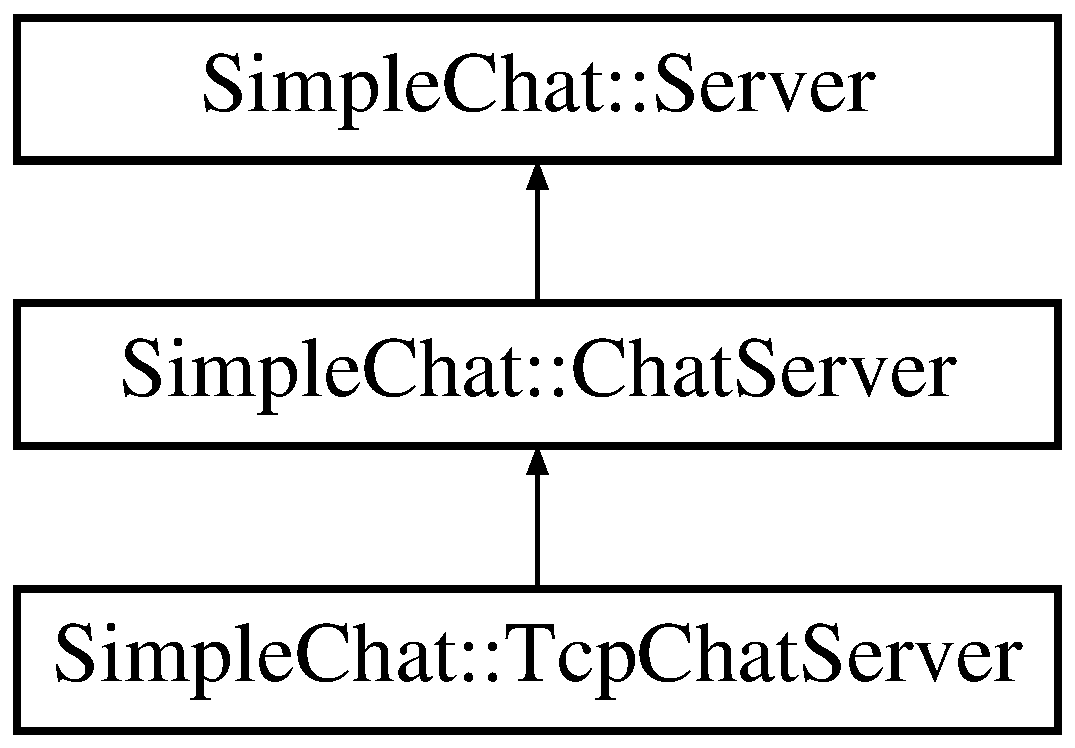
\includegraphics[height=3.000000cm]{classSimpleChat_1_1ChatServer}
\end{center}
\end{figure}
\subsection*{Public Member Functions}
\begin{DoxyCompactItemize}
\item 
\hypertarget{classSimpleChat_1_1ChatServer_a7f0056a5e7e352a16440fe4d1d5ff653}{{\bfseries Chat\-Server} (const std\-::string \&password)}\label{classSimpleChat_1_1ChatServer_a7f0056a5e7e352a16440fe4d1d5ff653}

\item 
\hypertarget{classSimpleChat_1_1ChatServer_aa47af706bc2dee5a9d446b53d0d04b00}{virtual void {\bfseries chatee\-Left} (const std\-::shared\-\_\-ptr$<$ \hyperlink{classSimpleChat_1_1Chatee}{Chatee} $>$ \&chatee) override}\label{classSimpleChat_1_1ChatServer_aa47af706bc2dee5a9d446b53d0d04b00}

\item 
\hypertarget{classSimpleChat_1_1ChatServer_a9b54ceb324dd24f9ab44217f8d5c4618}{virtual void {\bfseries handle\-Untyped\-Message} (const \hyperlink{classSimpleChat_1_1MessageDeserializer}{Message\-Deserializer} \&deserializer, \hyperlink{classSimpleChat_1_1ChatConnection}{Chat\-Connection} $\ast$connection) override}\label{classSimpleChat_1_1ChatServer_a9b54ceb324dd24f9ab44217f8d5c4618}

\item 
\hypertarget{classSimpleChat_1_1ChatServer_a4761fa8ac8451b2aed8bfe7f2b095cea}{virtual void {\bfseries handle\-Message} (std\-::unique\-\_\-ptr$<$ \hyperlink{classSimpleChat_1_1UserJoinRequest}{User\-Join\-Request} $>$ join\-Request, \hyperlink{classSimpleChat_1_1ChatConnection}{Chat\-Connection} $\ast$connection) override}\label{classSimpleChat_1_1ChatServer_a4761fa8ac8451b2aed8bfe7f2b095cea}

\item 
\hypertarget{classSimpleChat_1_1ChatServer_a6190e6309f6a01f87f8269c2756904f9}{virtual void {\bfseries handle\-Message} (std\-::unique\-\_\-ptr$<$ \hyperlink{classSimpleChat_1_1UserListRequest}{User\-List\-Request} $>$ list\-Request, const std\-::shared\-\_\-ptr$<$ \hyperlink{classSimpleChat_1_1Chatee}{Chatee} $>$ \&sender) override}\label{classSimpleChat_1_1ChatServer_a6190e6309f6a01f87f8269c2756904f9}

\item 
\hypertarget{classSimpleChat_1_1ChatServer_a7506c5bb2bf79b6d1fbac9c16e901f42}{virtual void {\bfseries handle\-Message} (std\-::unique\-\_\-ptr$<$ \hyperlink{classSimpleChat_1_1UserChange}{User\-Change} $>$ user\-Change, const std\-::shared\-\_\-ptr$<$ \hyperlink{classSimpleChat_1_1Chatee}{Chatee} $>$ \&sender) override}\label{classSimpleChat_1_1ChatServer_a7506c5bb2bf79b6d1fbac9c16e901f42}

\item 
virtual void \hyperlink{classSimpleChat_1_1ChatServer_aad034e6580f6898892e2289287261523}{handle\-Message} (std\-::unique\-\_\-ptr$<$ \hyperlink{classSimpleChat_1_1ChatMessage}{Chat\-Message} $>$ chat\-Message, const std\-::shared\-\_\-ptr$<$ \hyperlink{classSimpleChat_1_1Chatee}{Chatee} $>$ \&sender) override
\item 
\hypertarget{classSimpleChat_1_1ChatServer_ace617626c083e0a0ae36e74702335ff2}{virtual void {\bfseries handle\-Message} (std\-::unique\-\_\-ptr$<$ \hyperlink{classSimpleChat_1_1ChatCommand}{Chat\-Command} $>$ chat\-Command, const std\-::shared\-\_\-ptr$<$ \hyperlink{classSimpleChat_1_1Chatee}{Chatee} $>$ \&sender) override}\label{classSimpleChat_1_1ChatServer_ace617626c083e0a0ae36e74702335ff2}

\end{DoxyCompactItemize}
\subsection*{Protected Attributes}
\begin{DoxyCompactItemize}
\item 
\hypertarget{classSimpleChat_1_1ChatServer_a1b10f33b2e04c8b6a949ecff580aece7}{std\-::shared\-\_\-ptr$<$ \hyperlink{classSimpleChat_1_1Chatroom}{Chatroom} $>$ {\bfseries chatroom\-\_\-}}\label{classSimpleChat_1_1ChatServer_a1b10f33b2e04c8b6a949ecff580aece7}

\item 
\hypertarget{classSimpleChat_1_1ChatServer_a0edc2731025fd3cc11014ad07277bda1}{std\-::string {\bfseries password\-\_\-}}\label{classSimpleChat_1_1ChatServer_a0edc2731025fd3cc11014ad07277bda1}

\end{DoxyCompactItemize}


\subsection{Member Function Documentation}
\hypertarget{classSimpleChat_1_1ChatServer_aad034e6580f6898892e2289287261523}{\index{Simple\-Chat\-::\-Chat\-Server@{Simple\-Chat\-::\-Chat\-Server}!handle\-Message@{handle\-Message}}
\index{handle\-Message@{handle\-Message}!SimpleChat::ChatServer@{Simple\-Chat\-::\-Chat\-Server}}
\subsubsection[{handle\-Message}]{\setlength{\rightskip}{0pt plus 5cm}void Simple\-Chat\-::\-Chat\-Server\-::handle\-Message (
\begin{DoxyParamCaption}
\item[{std\-::unique\-\_\-ptr$<$ {\bf Chat\-Message} $>$}]{chat\-Message, }
\item[{const std\-::shared\-\_\-ptr$<$ {\bf Chatee} $>$ \&}]{sender}
\end{DoxyParamCaption}
)\hspace{0.3cm}{\ttfamily [override]}, {\ttfamily [virtual]}}}\label{classSimpleChat_1_1ChatServer_aad034e6580f6898892e2289287261523}
send a private message

let the sender know that target doesn't exist

tell sender -\/ message from sender to target was sent

tell target -\/ message from sender was received

send a public message

check if the user is muted 

Implements \hyperlink{classSimpleChat_1_1Server}{Simple\-Chat\-::\-Server}.



The documentation for this class was generated from the following files\-:\begin{DoxyCompactItemize}
\item 
chatlib/server/Chat\-Server.\-h\item 
chatlib/server/Chat\-Server.\-cpp\end{DoxyCompactItemize}

\hypertarget{classSimpleChat_1_1ChatTarget}{\section{Simple\-Chat\-:\-:Chat\-Target Class Reference}
\label{classSimpleChat_1_1ChatTarget}\index{Simple\-Chat\-::\-Chat\-Target@{Simple\-Chat\-::\-Chat\-Target}}
}
Inheritance diagram for Simple\-Chat\-:\-:Chat\-Target\-:\begin{figure}[H]
\begin{center}
\leavevmode
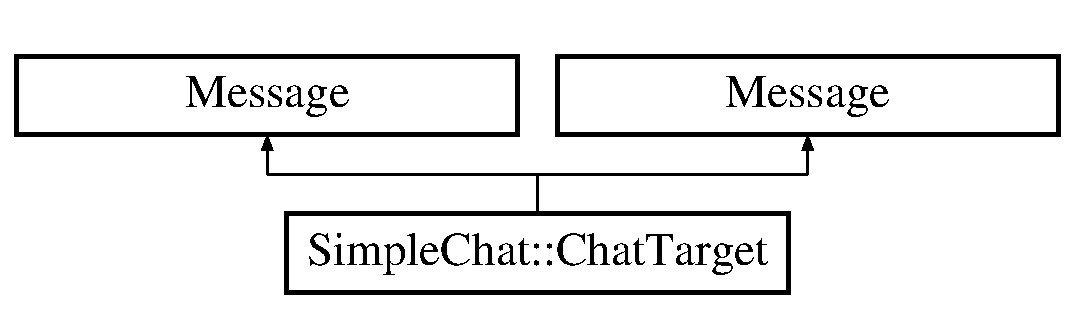
\includegraphics[height=2.000000cm]{classSimpleChat_1_1ChatTarget}
\end{center}
\end{figure}
\subsection*{Public Member Functions}
\begin{DoxyCompactItemize}
\item 
\hypertarget{classSimpleChat_1_1ChatTarget_a15dc4f81b37b35fa79f8b8b2a9e343bb}{{\bfseries Chat\-Target} (const \hyperlink{classSimpleChat_1_1ChatTarget}{Chat\-Target} \&from)}\label{classSimpleChat_1_1ChatTarget_a15dc4f81b37b35fa79f8b8b2a9e343bb}

\item 
\hypertarget{classSimpleChat_1_1ChatTarget_a5c22124ec3d1affa15f661f4fef9eba9}{\hyperlink{classSimpleChat_1_1ChatTarget}{Chat\-Target} \& {\bfseries operator=} (const \hyperlink{classSimpleChat_1_1ChatTarget}{Chat\-Target} \&from)}\label{classSimpleChat_1_1ChatTarget_a5c22124ec3d1affa15f661f4fef9eba9}

\item 
\hypertarget{classSimpleChat_1_1ChatTarget_a8f89893fda6f9746dded787b9c65a7a5}{const \\*
\-::google\-::protobuf\-::\-Unknown\-Field\-Set \& {\bfseries unknown\-\_\-fields} () const }\label{classSimpleChat_1_1ChatTarget_a8f89893fda6f9746dded787b9c65a7a5}

\item 
\hypertarget{classSimpleChat_1_1ChatTarget_aab4226f6d671e5e4a008bd5e889aa322}{inline\-::google\-::protobuf\-::\-Unknown\-Field\-Set $\ast$ {\bfseries mutable\-\_\-unknown\-\_\-fields} ()}\label{classSimpleChat_1_1ChatTarget_aab4226f6d671e5e4a008bd5e889aa322}

\item 
\hypertarget{classSimpleChat_1_1ChatTarget_a94869595abb80310c9be52a3003bfac6}{void {\bfseries Swap} (\hyperlink{classSimpleChat_1_1ChatTarget}{Chat\-Target} $\ast$other)}\label{classSimpleChat_1_1ChatTarget_a94869595abb80310c9be52a3003bfac6}

\item 
\hypertarget{classSimpleChat_1_1ChatTarget_ad04e89f9a6180979b13d06ffdbcc6e33}{\hyperlink{classSimpleChat_1_1ChatTarget}{Chat\-Target} $\ast$ {\bfseries New} () const }\label{classSimpleChat_1_1ChatTarget_ad04e89f9a6180979b13d06ffdbcc6e33}

\item 
\hypertarget{classSimpleChat_1_1ChatTarget_ad83821f89032d4bd3ca0b9b75c12c8fb}{\hyperlink{classSimpleChat_1_1ChatTarget}{Chat\-Target} $\ast$ {\bfseries New} (\-::google\-::protobuf\-::\-Arena $\ast$arena) const }\label{classSimpleChat_1_1ChatTarget_ad83821f89032d4bd3ca0b9b75c12c8fb}

\item 
\hypertarget{classSimpleChat_1_1ChatTarget_a94d55ead775ccd548848efefc4e18509}{void {\bfseries Copy\-From} (const \-::google\-::protobuf\-::\-Message \&from)}\label{classSimpleChat_1_1ChatTarget_a94d55ead775ccd548848efefc4e18509}

\item 
\hypertarget{classSimpleChat_1_1ChatTarget_ac65c80b3519e88a89c1531c768f051d4}{void {\bfseries Merge\-From} (const \-::google\-::protobuf\-::\-Message \&from)}\label{classSimpleChat_1_1ChatTarget_ac65c80b3519e88a89c1531c768f051d4}

\item 
\hypertarget{classSimpleChat_1_1ChatTarget_a1852d72c18ee6ca3a6a6237ee6e6e49c}{void {\bfseries Copy\-From} (const \hyperlink{classSimpleChat_1_1ChatTarget}{Chat\-Target} \&from)}\label{classSimpleChat_1_1ChatTarget_a1852d72c18ee6ca3a6a6237ee6e6e49c}

\item 
\hypertarget{classSimpleChat_1_1ChatTarget_aea2cc4d829f43be963fe5e5281c58b88}{void {\bfseries Merge\-From} (const \hyperlink{classSimpleChat_1_1ChatTarget}{Chat\-Target} \&from)}\label{classSimpleChat_1_1ChatTarget_aea2cc4d829f43be963fe5e5281c58b88}

\item 
\hypertarget{classSimpleChat_1_1ChatTarget_a0172176ef83d2e89f8e42e76021b8519}{void {\bfseries Clear} ()}\label{classSimpleChat_1_1ChatTarget_a0172176ef83d2e89f8e42e76021b8519}

\item 
\hypertarget{classSimpleChat_1_1ChatTarget_aa8e4da7087df9548ab7e20909b9b4ccd}{bool {\bfseries Is\-Initialized} () const }\label{classSimpleChat_1_1ChatTarget_aa8e4da7087df9548ab7e20909b9b4ccd}

\item 
\hypertarget{classSimpleChat_1_1ChatTarget_a9437724d77d2202440b3bb4e04f170cf}{int {\bfseries Byte\-Size} () const }\label{classSimpleChat_1_1ChatTarget_a9437724d77d2202440b3bb4e04f170cf}

\item 
\hypertarget{classSimpleChat_1_1ChatTarget_ab35d0ebdf526a521e3022d723abef84b}{bool {\bfseries Merge\-Partial\-From\-Coded\-Stream} (\-::google\-::protobuf\-::io\-::\-Coded\-Input\-Stream $\ast$input)}\label{classSimpleChat_1_1ChatTarget_ab35d0ebdf526a521e3022d723abef84b}

\item 
\hypertarget{classSimpleChat_1_1ChatTarget_a0e9d4cbc640da603feaebccbf1205115}{void {\bfseries Serialize\-With\-Cached\-Sizes} (\-::google\-::protobuf\-::io\-::\-Coded\-Output\-Stream $\ast$output) const }\label{classSimpleChat_1_1ChatTarget_a0e9d4cbc640da603feaebccbf1205115}

\item 
\hypertarget{classSimpleChat_1_1ChatTarget_a571dabbabfa13682a417763cf8295430}{\-::google\-::protobuf\-::uint8 $\ast$ {\bfseries Serialize\-With\-Cached\-Sizes\-To\-Array} (\-::google\-::protobuf\-::uint8 $\ast$output) const }\label{classSimpleChat_1_1ChatTarget_a571dabbabfa13682a417763cf8295430}

\item 
\hypertarget{classSimpleChat_1_1ChatTarget_ae7f5a171f96de9e6f48a5d066160b3af}{int {\bfseries Get\-Cached\-Size} () const }\label{classSimpleChat_1_1ChatTarget_ae7f5a171f96de9e6f48a5d066160b3af}

\item 
\hypertarget{classSimpleChat_1_1ChatTarget_aff7a0f604becdbd2c8c431741f38f48e}{\-::google\-::protobuf\-::\-Metadata {\bfseries Get\-Metadata} () const }\label{classSimpleChat_1_1ChatTarget_aff7a0f604becdbd2c8c431741f38f48e}

\item 
\hypertarget{classSimpleChat_1_1ChatTarget_a66e0bc40c78d2b66c9fb9afbf2c5953e}{bool {\bfseries has\-\_\-user\-\_\-name} () const }\label{classSimpleChat_1_1ChatTarget_a66e0bc40c78d2b66c9fb9afbf2c5953e}

\item 
\hypertarget{classSimpleChat_1_1ChatTarget_aabc592535549d57aeb35790ba8a082aa}{void {\bfseries clear\-\_\-user\-\_\-name} ()}\label{classSimpleChat_1_1ChatTarget_aabc592535549d57aeb35790ba8a082aa}

\item 
\hypertarget{classSimpleChat_1_1ChatTarget_a0e7fecd185ef684d2a11bbd0d40288f4}{const \-::std\-::string \& {\bfseries user\-\_\-name} () const }\label{classSimpleChat_1_1ChatTarget_a0e7fecd185ef684d2a11bbd0d40288f4}

\item 
\hypertarget{classSimpleChat_1_1ChatTarget_ae0dfb8025905103704facea22ff305fd}{void {\bfseries set\-\_\-user\-\_\-name} (const \-::std\-::string \&value)}\label{classSimpleChat_1_1ChatTarget_ae0dfb8025905103704facea22ff305fd}

\item 
\hypertarget{classSimpleChat_1_1ChatTarget_a1853ab22e4f8153ceca6e764c9b2b3bc}{void {\bfseries set\-\_\-user\-\_\-name} (const char $\ast$value)}\label{classSimpleChat_1_1ChatTarget_a1853ab22e4f8153ceca6e764c9b2b3bc}

\item 
\hypertarget{classSimpleChat_1_1ChatTarget_a3d3431afad65e465a73cff3bc9b466fb}{void {\bfseries set\-\_\-user\-\_\-name} (const char $\ast$value, size\-\_\-t size)}\label{classSimpleChat_1_1ChatTarget_a3d3431afad65e465a73cff3bc9b466fb}

\item 
\hypertarget{classSimpleChat_1_1ChatTarget_a00afe8502b37643f560038dea704e5ff}{\-::std\-::string $\ast$ {\bfseries mutable\-\_\-user\-\_\-name} ()}\label{classSimpleChat_1_1ChatTarget_a00afe8502b37643f560038dea704e5ff}

\item 
\hypertarget{classSimpleChat_1_1ChatTarget_a7156ab60121584ae5364003f778588fe}{\-::std\-::string $\ast$ {\bfseries release\-\_\-user\-\_\-name} ()}\label{classSimpleChat_1_1ChatTarget_a7156ab60121584ae5364003f778588fe}

\item 
\hypertarget{classSimpleChat_1_1ChatTarget_a82559c41d4d25af52c6a5f83814eac69}{void {\bfseries set\-\_\-allocated\-\_\-user\-\_\-name} (\-::std\-::string $\ast$user\-\_\-name)}\label{classSimpleChat_1_1ChatTarget_a82559c41d4d25af52c6a5f83814eac69}

\item 
\hypertarget{classSimpleChat_1_1ChatTarget_a0831d25def649fe153f0e3075bbbfac6}{bool {\bfseries has\-\_\-user\-\_\-id} () const }\label{classSimpleChat_1_1ChatTarget_a0831d25def649fe153f0e3075bbbfac6}

\item 
\hypertarget{classSimpleChat_1_1ChatTarget_a0e07f02eeb547853bdce8e2745d55fd2}{void {\bfseries clear\-\_\-user\-\_\-id} ()}\label{classSimpleChat_1_1ChatTarget_a0e07f02eeb547853bdce8e2745d55fd2}

\item 
\hypertarget{classSimpleChat_1_1ChatTarget_a7e162e2a192107d514d2350c3ae190d2}{\-::google\-::protobuf\-::int32 {\bfseries user\-\_\-id} () const }\label{classSimpleChat_1_1ChatTarget_a7e162e2a192107d514d2350c3ae190d2}

\item 
\hypertarget{classSimpleChat_1_1ChatTarget_aa8851c988d1010b224705df2a4889116}{void {\bfseries set\-\_\-user\-\_\-id} (\-::google\-::protobuf\-::int32 value)}\label{classSimpleChat_1_1ChatTarget_aa8851c988d1010b224705df2a4889116}

\item 
\hypertarget{classSimpleChat_1_1ChatTarget_a15dc4f81b37b35fa79f8b8b2a9e343bb}{{\bfseries Chat\-Target} (const \hyperlink{classSimpleChat_1_1ChatTarget}{Chat\-Target} \&from)}\label{classSimpleChat_1_1ChatTarget_a15dc4f81b37b35fa79f8b8b2a9e343bb}

\item 
\hypertarget{classSimpleChat_1_1ChatTarget_a5c22124ec3d1affa15f661f4fef9eba9}{\hyperlink{classSimpleChat_1_1ChatTarget}{Chat\-Target} \& {\bfseries operator=} (const \hyperlink{classSimpleChat_1_1ChatTarget}{Chat\-Target} \&from)}\label{classSimpleChat_1_1ChatTarget_a5c22124ec3d1affa15f661f4fef9eba9}

\item 
\hypertarget{classSimpleChat_1_1ChatTarget_a8f89893fda6f9746dded787b9c65a7a5}{const \\*
\-::google\-::protobuf\-::\-Unknown\-Field\-Set \& {\bfseries unknown\-\_\-fields} () const }\label{classSimpleChat_1_1ChatTarget_a8f89893fda6f9746dded787b9c65a7a5}

\item 
\hypertarget{classSimpleChat_1_1ChatTarget_aab4226f6d671e5e4a008bd5e889aa322}{inline\-::google\-::protobuf\-::\-Unknown\-Field\-Set $\ast$ {\bfseries mutable\-\_\-unknown\-\_\-fields} ()}\label{classSimpleChat_1_1ChatTarget_aab4226f6d671e5e4a008bd5e889aa322}

\item 
\hypertarget{classSimpleChat_1_1ChatTarget_a94869595abb80310c9be52a3003bfac6}{void {\bfseries Swap} (\hyperlink{classSimpleChat_1_1ChatTarget}{Chat\-Target} $\ast$other)}\label{classSimpleChat_1_1ChatTarget_a94869595abb80310c9be52a3003bfac6}

\item 
\hypertarget{classSimpleChat_1_1ChatTarget_ad04e89f9a6180979b13d06ffdbcc6e33}{\hyperlink{classSimpleChat_1_1ChatTarget}{Chat\-Target} $\ast$ {\bfseries New} () const }\label{classSimpleChat_1_1ChatTarget_ad04e89f9a6180979b13d06ffdbcc6e33}

\item 
\hypertarget{classSimpleChat_1_1ChatTarget_ad83821f89032d4bd3ca0b9b75c12c8fb}{\hyperlink{classSimpleChat_1_1ChatTarget}{Chat\-Target} $\ast$ {\bfseries New} (\-::google\-::protobuf\-::\-Arena $\ast$arena) const }\label{classSimpleChat_1_1ChatTarget_ad83821f89032d4bd3ca0b9b75c12c8fb}

\item 
\hypertarget{classSimpleChat_1_1ChatTarget_a94d55ead775ccd548848efefc4e18509}{void {\bfseries Copy\-From} (const \-::google\-::protobuf\-::\-Message \&from)}\label{classSimpleChat_1_1ChatTarget_a94d55ead775ccd548848efefc4e18509}

\item 
\hypertarget{classSimpleChat_1_1ChatTarget_ac65c80b3519e88a89c1531c768f051d4}{void {\bfseries Merge\-From} (const \-::google\-::protobuf\-::\-Message \&from)}\label{classSimpleChat_1_1ChatTarget_ac65c80b3519e88a89c1531c768f051d4}

\item 
\hypertarget{classSimpleChat_1_1ChatTarget_a1852d72c18ee6ca3a6a6237ee6e6e49c}{void {\bfseries Copy\-From} (const \hyperlink{classSimpleChat_1_1ChatTarget}{Chat\-Target} \&from)}\label{classSimpleChat_1_1ChatTarget_a1852d72c18ee6ca3a6a6237ee6e6e49c}

\item 
\hypertarget{classSimpleChat_1_1ChatTarget_aea2cc4d829f43be963fe5e5281c58b88}{void {\bfseries Merge\-From} (const \hyperlink{classSimpleChat_1_1ChatTarget}{Chat\-Target} \&from)}\label{classSimpleChat_1_1ChatTarget_aea2cc4d829f43be963fe5e5281c58b88}

\item 
\hypertarget{classSimpleChat_1_1ChatTarget_a0172176ef83d2e89f8e42e76021b8519}{void {\bfseries Clear} ()}\label{classSimpleChat_1_1ChatTarget_a0172176ef83d2e89f8e42e76021b8519}

\item 
\hypertarget{classSimpleChat_1_1ChatTarget_aa8e4da7087df9548ab7e20909b9b4ccd}{bool {\bfseries Is\-Initialized} () const }\label{classSimpleChat_1_1ChatTarget_aa8e4da7087df9548ab7e20909b9b4ccd}

\item 
\hypertarget{classSimpleChat_1_1ChatTarget_a9437724d77d2202440b3bb4e04f170cf}{int {\bfseries Byte\-Size} () const }\label{classSimpleChat_1_1ChatTarget_a9437724d77d2202440b3bb4e04f170cf}

\item 
\hypertarget{classSimpleChat_1_1ChatTarget_ab35d0ebdf526a521e3022d723abef84b}{bool {\bfseries Merge\-Partial\-From\-Coded\-Stream} (\-::google\-::protobuf\-::io\-::\-Coded\-Input\-Stream $\ast$input)}\label{classSimpleChat_1_1ChatTarget_ab35d0ebdf526a521e3022d723abef84b}

\item 
\hypertarget{classSimpleChat_1_1ChatTarget_a0e9d4cbc640da603feaebccbf1205115}{void {\bfseries Serialize\-With\-Cached\-Sizes} (\-::google\-::protobuf\-::io\-::\-Coded\-Output\-Stream $\ast$output) const }\label{classSimpleChat_1_1ChatTarget_a0e9d4cbc640da603feaebccbf1205115}

\item 
\hypertarget{classSimpleChat_1_1ChatTarget_a571dabbabfa13682a417763cf8295430}{\-::google\-::protobuf\-::uint8 $\ast$ {\bfseries Serialize\-With\-Cached\-Sizes\-To\-Array} (\-::google\-::protobuf\-::uint8 $\ast$output) const }\label{classSimpleChat_1_1ChatTarget_a571dabbabfa13682a417763cf8295430}

\item 
\hypertarget{classSimpleChat_1_1ChatTarget_ae7f5a171f96de9e6f48a5d066160b3af}{int {\bfseries Get\-Cached\-Size} () const }\label{classSimpleChat_1_1ChatTarget_ae7f5a171f96de9e6f48a5d066160b3af}

\item 
\hypertarget{classSimpleChat_1_1ChatTarget_aff7a0f604becdbd2c8c431741f38f48e}{\-::google\-::protobuf\-::\-Metadata {\bfseries Get\-Metadata} () const }\label{classSimpleChat_1_1ChatTarget_aff7a0f604becdbd2c8c431741f38f48e}

\item 
\hypertarget{classSimpleChat_1_1ChatTarget_a66e0bc40c78d2b66c9fb9afbf2c5953e}{bool {\bfseries has\-\_\-user\-\_\-name} () const }\label{classSimpleChat_1_1ChatTarget_a66e0bc40c78d2b66c9fb9afbf2c5953e}

\item 
\hypertarget{classSimpleChat_1_1ChatTarget_aabc592535549d57aeb35790ba8a082aa}{void {\bfseries clear\-\_\-user\-\_\-name} ()}\label{classSimpleChat_1_1ChatTarget_aabc592535549d57aeb35790ba8a082aa}

\item 
\hypertarget{classSimpleChat_1_1ChatTarget_a9a4f84c9215e5e3f6b8cbe325008632e}{const \-::std\-::string \& {\bfseries user\-\_\-name} () const }\label{classSimpleChat_1_1ChatTarget_a9a4f84c9215e5e3f6b8cbe325008632e}

\item 
\hypertarget{classSimpleChat_1_1ChatTarget_ae0dfb8025905103704facea22ff305fd}{void {\bfseries set\-\_\-user\-\_\-name} (const \-::std\-::string \&value)}\label{classSimpleChat_1_1ChatTarget_ae0dfb8025905103704facea22ff305fd}

\item 
\hypertarget{classSimpleChat_1_1ChatTarget_a1853ab22e4f8153ceca6e764c9b2b3bc}{void {\bfseries set\-\_\-user\-\_\-name} (const char $\ast$value)}\label{classSimpleChat_1_1ChatTarget_a1853ab22e4f8153ceca6e764c9b2b3bc}

\item 
\hypertarget{classSimpleChat_1_1ChatTarget_a3d3431afad65e465a73cff3bc9b466fb}{void {\bfseries set\-\_\-user\-\_\-name} (const char $\ast$value, size\-\_\-t size)}\label{classSimpleChat_1_1ChatTarget_a3d3431afad65e465a73cff3bc9b466fb}

\item 
\hypertarget{classSimpleChat_1_1ChatTarget_ab5f2b7a7ca18ba806baf74e55cab4ff3}{\-::std\-::string $\ast$ {\bfseries mutable\-\_\-user\-\_\-name} ()}\label{classSimpleChat_1_1ChatTarget_ab5f2b7a7ca18ba806baf74e55cab4ff3}

\item 
\hypertarget{classSimpleChat_1_1ChatTarget_a0ce718bcee6d70ec92bf5e0b74b10f7d}{\-::std\-::string $\ast$ {\bfseries release\-\_\-user\-\_\-name} ()}\label{classSimpleChat_1_1ChatTarget_a0ce718bcee6d70ec92bf5e0b74b10f7d}

\item 
\hypertarget{classSimpleChat_1_1ChatTarget_a82559c41d4d25af52c6a5f83814eac69}{void {\bfseries set\-\_\-allocated\-\_\-user\-\_\-name} (\-::std\-::string $\ast$user\-\_\-name)}\label{classSimpleChat_1_1ChatTarget_a82559c41d4d25af52c6a5f83814eac69}

\item 
\hypertarget{classSimpleChat_1_1ChatTarget_a0831d25def649fe153f0e3075bbbfac6}{bool {\bfseries has\-\_\-user\-\_\-id} () const }\label{classSimpleChat_1_1ChatTarget_a0831d25def649fe153f0e3075bbbfac6}

\item 
\hypertarget{classSimpleChat_1_1ChatTarget_a0e07f02eeb547853bdce8e2745d55fd2}{void {\bfseries clear\-\_\-user\-\_\-id} ()}\label{classSimpleChat_1_1ChatTarget_a0e07f02eeb547853bdce8e2745d55fd2}

\item 
\hypertarget{classSimpleChat_1_1ChatTarget_a38f80ef4a9b6dd30d4c6f93657f9230e}{\-::google\-::protobuf\-::int32 {\bfseries user\-\_\-id} () const }\label{classSimpleChat_1_1ChatTarget_a38f80ef4a9b6dd30d4c6f93657f9230e}

\item 
\hypertarget{classSimpleChat_1_1ChatTarget_aa8851c988d1010b224705df2a4889116}{void {\bfseries set\-\_\-user\-\_\-id} (\-::google\-::protobuf\-::int32 value)}\label{classSimpleChat_1_1ChatTarget_aa8851c988d1010b224705df2a4889116}

\end{DoxyCompactItemize}
\subsection*{Static Public Member Functions}
\begin{DoxyCompactItemize}
\item 
\hypertarget{classSimpleChat_1_1ChatTarget_a7d09d1903755f3b96eb4dfa5cb654cb5}{static const \\*
\-::google\-::protobuf\-::\-Descriptor $\ast$ {\bfseries descriptor} ()}\label{classSimpleChat_1_1ChatTarget_a7d09d1903755f3b96eb4dfa5cb654cb5}

\item 
\hypertarget{classSimpleChat_1_1ChatTarget_ac0fbbc1763163ab89e04a6fc776ce59f}{static const \hyperlink{classSimpleChat_1_1ChatTarget}{Chat\-Target} \& {\bfseries default\-\_\-instance} ()}\label{classSimpleChat_1_1ChatTarget_ac0fbbc1763163ab89e04a6fc776ce59f}

\item 
\hypertarget{classSimpleChat_1_1ChatTarget_a7d09d1903755f3b96eb4dfa5cb654cb5}{static const \\*
\-::google\-::protobuf\-::\-Descriptor $\ast$ {\bfseries descriptor} ()}\label{classSimpleChat_1_1ChatTarget_a7d09d1903755f3b96eb4dfa5cb654cb5}

\item 
\hypertarget{classSimpleChat_1_1ChatTarget_ac0fbbc1763163ab89e04a6fc776ce59f}{static const \hyperlink{classSimpleChat_1_1ChatTarget}{Chat\-Target} \& {\bfseries default\-\_\-instance} ()}\label{classSimpleChat_1_1ChatTarget_ac0fbbc1763163ab89e04a6fc776ce59f}

\end{DoxyCompactItemize}
\subsection*{Static Public Attributes}
\begin{DoxyCompactItemize}
\item 
\hypertarget{classSimpleChat_1_1ChatTarget_a1ab7dc5d077b8b447dec63fef8dd08b3}{static const int {\bfseries k\-User\-Name\-Field\-Number} = 1}\label{classSimpleChat_1_1ChatTarget_a1ab7dc5d077b8b447dec63fef8dd08b3}

\item 
\hypertarget{classSimpleChat_1_1ChatTarget_a9bfaf7a0f8b951b2f968a804f7b2c179}{static const int {\bfseries k\-User\-Id\-Field\-Number} = 2}\label{classSimpleChat_1_1ChatTarget_a9bfaf7a0f8b951b2f968a804f7b2c179}

\end{DoxyCompactItemize}
\subsection*{Friends}
\begin{DoxyCompactItemize}
\item 
\hypertarget{classSimpleChat_1_1ChatTarget_ab0d9593aa41361f04ab91f917ef9ec0e}{void {\bfseries protobuf\-\_\-\-Add\-Desc\-\_\-\-Chat\-Message\-\_\-2eproto} ()}\label{classSimpleChat_1_1ChatTarget_ab0d9593aa41361f04ab91f917ef9ec0e}

\item 
\hypertarget{classSimpleChat_1_1ChatTarget_a4ca7b2c64786782406ca69f6ba39ccb2}{void {\bfseries protobuf\-\_\-\-Assign\-Desc\-\_\-\-Chat\-Message\-\_\-2eproto} ()}\label{classSimpleChat_1_1ChatTarget_a4ca7b2c64786782406ca69f6ba39ccb2}

\item 
\hypertarget{classSimpleChat_1_1ChatTarget_a78726b79d52a130a50d7670a5c0238fc}{void {\bfseries protobuf\-\_\-\-Shutdown\-File\-\_\-\-Chat\-Message\-\_\-2eproto} ()}\label{classSimpleChat_1_1ChatTarget_a78726b79d52a130a50d7670a5c0238fc}

\item 
\hypertarget{classSimpleChat_1_1ChatTarget_ab0d9593aa41361f04ab91f917ef9ec0e}{void {\bfseries protobuf\-\_\-\-Add\-Desc\-\_\-\-Chat\-Message\-\_\-2eproto} ()}\label{classSimpleChat_1_1ChatTarget_ab0d9593aa41361f04ab91f917ef9ec0e}

\item 
\hypertarget{classSimpleChat_1_1ChatTarget_a4ca7b2c64786782406ca69f6ba39ccb2}{void {\bfseries protobuf\-\_\-\-Assign\-Desc\-\_\-\-Chat\-Message\-\_\-2eproto} ()}\label{classSimpleChat_1_1ChatTarget_a4ca7b2c64786782406ca69f6ba39ccb2}

\item 
\hypertarget{classSimpleChat_1_1ChatTarget_a78726b79d52a130a50d7670a5c0238fc}{void {\bfseries protobuf\-\_\-\-Shutdown\-File\-\_\-\-Chat\-Message\-\_\-2eproto} ()}\label{classSimpleChat_1_1ChatTarget_a78726b79d52a130a50d7670a5c0238fc}

\end{DoxyCompactItemize}


The documentation for this class was generated from the following file\-:\begin{DoxyCompactItemize}
\item 
chatlib/proto/Chat\-Message.\-pb.\-h\end{DoxyCompactItemize}

\hypertarget{classSimpleChat_1_1Client}{\section{Simple\-Chat\-:\-:Client Class Reference}
\label{classSimpleChat_1_1Client}\index{Simple\-Chat\-::\-Client@{Simple\-Chat\-::\-Client}}
}
Inheritance diagram for Simple\-Chat\-:\-:Client\-:\begin{figure}[H]
\begin{center}
\leavevmode
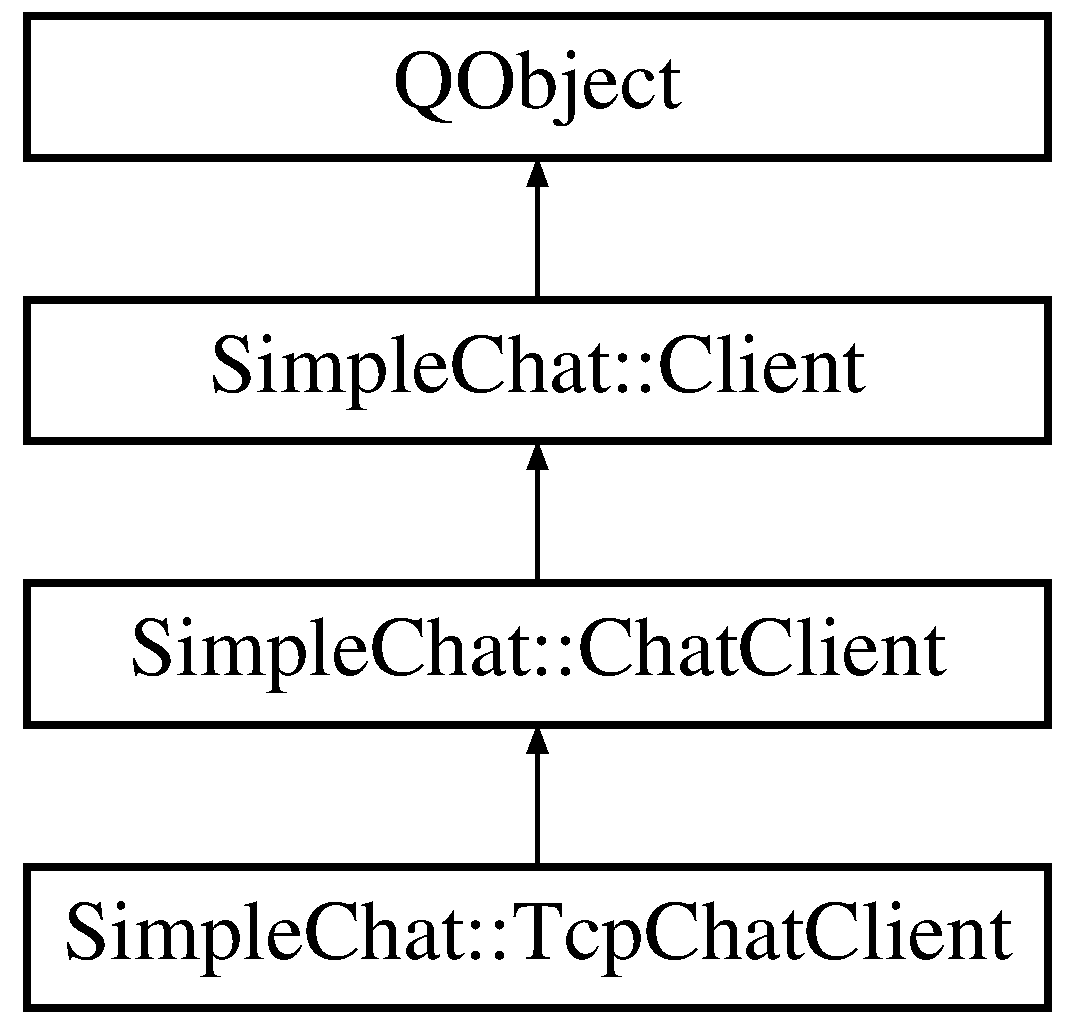
\includegraphics[height=4.000000cm]{classSimpleChat_1_1Client}
\end{center}
\end{figure}
\subsection*{Signals}
\begin{DoxyCompactItemize}
\item 
\hypertarget{classSimpleChat_1_1Client_af340df83298809f010245e79848566ff}{void {\bfseries new\-Message} (const Q\-String \&from, const Q\-String \&message)}\label{classSimpleChat_1_1Client_af340df83298809f010245e79848566ff}

\item 
\hypertarget{classSimpleChat_1_1Client_ad5cb656ab4f18f8299ece913c880e484}{void {\bfseries new\-Participant} (const Q\-String \&nick)}\label{classSimpleChat_1_1Client_ad5cb656ab4f18f8299ece913c880e484}

\item 
\hypertarget{classSimpleChat_1_1Client_a84c8aa20f1476230237234bc0d35df28}{void {\bfseries participant\-Left} (const Q\-String \&nick)}\label{classSimpleChat_1_1Client_a84c8aa20f1476230237234bc0d35df28}

\end{DoxyCompactItemize}
\subsection*{Public Member Functions}
\begin{DoxyCompactItemize}
\item 
\hypertarget{classSimpleChat_1_1Client_afc4e5a32a2c8b9c9522ead7f101a3629}{virtual bool {\bfseries send\-Command} (const std\-::string \&command)=0}\label{classSimpleChat_1_1Client_afc4e5a32a2c8b9c9522ead7f101a3629}

\item 
\hypertarget{classSimpleChat_1_1Client_ad0504f9d44fc4a2e9bc467aa7beb0950}{virtual void {\bfseries send\-Message} (const std\-::string \&text, const std\-::string \&target)=0}\label{classSimpleChat_1_1Client_ad0504f9d44fc4a2e9bc467aa7beb0950}

\item 
\hypertarget{classSimpleChat_1_1Client_ad0b8c66ae9d8eb6a03922381da5cacb7}{virtual void {\bfseries handle\-Untyped\-Message} (const \hyperlink{classSimpleChat_1_1MessageDeserializer}{Message\-Deserializer} \&deserializer)=0}\label{classSimpleChat_1_1Client_ad0b8c66ae9d8eb6a03922381da5cacb7}

\item 
\hypertarget{classSimpleChat_1_1Client_a8de58147fb0d696d936fb890de16532b}{virtual void {\bfseries handle\-Message} (std\-::unique\-\_\-ptr$<$ \hyperlink{classSimpleChat_1_1UserJoinResponse}{User\-Join\-Response} $>$ join\-Response)=0}\label{classSimpleChat_1_1Client_a8de58147fb0d696d936fb890de16532b}

\item 
\hypertarget{classSimpleChat_1_1Client_a217efb7a31801a0b67513f88a45bd008}{virtual void {\bfseries handle\-Message} (std\-::unique\-\_\-ptr$<$ \hyperlink{classSimpleChat_1_1UserListResponse}{User\-List\-Response} $>$ list\-Response)=0}\label{classSimpleChat_1_1Client_a217efb7a31801a0b67513f88a45bd008}

\item 
\hypertarget{classSimpleChat_1_1Client_a764eb53f0c377f3a6b7bd7e969ed3836}{virtual void {\bfseries handle\-Message} (std\-::unique\-\_\-ptr$<$ \hyperlink{classSimpleChat_1_1UserChange}{User\-Change} $>$ user\-Change)=0}\label{classSimpleChat_1_1Client_a764eb53f0c377f3a6b7bd7e969ed3836}

\item 
\hypertarget{classSimpleChat_1_1Client_af23c5866ac9992d98afd4cd6a71da0cd}{virtual void {\bfseries handle\-Message} (std\-::unique\-\_\-ptr$<$ \hyperlink{classSimpleChat_1_1ChatMessage}{Chat\-Message} $>$ chat\-Message)=0}\label{classSimpleChat_1_1Client_af23c5866ac9992d98afd4cd6a71da0cd}

\item 
\hypertarget{classSimpleChat_1_1Client_a235dfb2fb833d30ae89b45d137e2b213}{virtual void {\bfseries handle\-Message} (std\-::unique\-\_\-ptr$<$ \hyperlink{classSimpleChat_1_1ChatroomChange}{Chatroom\-Change} $>$ chatroom\-Change)=0}\label{classSimpleChat_1_1Client_a235dfb2fb833d30ae89b45d137e2b213}

\item 
\hypertarget{classSimpleChat_1_1Client_abb550a7e0ca6b2cd238ac260280554f6}{virtual void {\bfseries handle\-Message} (std\-::unique\-\_\-ptr$<$ \hyperlink{classSimpleChat_1_1GenericChatResponse}{Generic\-Chat\-Response} $>$ response)=0}\label{classSimpleChat_1_1Client_abb550a7e0ca6b2cd238ac260280554f6}

\item 
\hypertarget{classSimpleChat_1_1Client_ae43df7f8403aa1f21ef11e3ded5f808f}{virtual std\-::string {\bfseries name} ()=0}\label{classSimpleChat_1_1Client_ae43df7f8403aa1f21ef11e3ded5f808f}

\item 
\hypertarget{classSimpleChat_1_1Client_a288256d4752a558bbaeb5923b5764f31}{void {\bfseries send\-Message} (const Q\-String \&message)}\label{classSimpleChat_1_1Client_a288256d4752a558bbaeb5923b5764f31}

\item 
\hypertarget{classSimpleChat_1_1Client_a9c42ea3b937cd82970e45ab8f54e3f4a}{Q\-String {\bfseries nick\-Name} () const }\label{classSimpleChat_1_1Client_a9c42ea3b937cd82970e45ab8f54e3f4a}

\item 
\hypertarget{classSimpleChat_1_1Client_a11d8ef0ed9f8b3faf08f300452d334fd}{bool {\bfseries has\-Connection} (const Q\-Host\-Address \&sender\-Ip, int sender\-Port=-\/1) const }\label{classSimpleChat_1_1Client_a11d8ef0ed9f8b3faf08f300452d334fd}

\end{DoxyCompactItemize}
\subsection*{Protected Member Functions}
\begin{DoxyCompactItemize}
\item 
\hypertarget{classSimpleChat_1_1Client_a19905e07f2ac81e2ca87d34f3c33b644}{virtual bool {\bfseries send\-Any\-Message} (std\-::unique\-\_\-ptr$<$ \hyperlink{classSimpleChat_1_1AbstractMessage}{Abstract\-Message} $>$ message)=0}\label{classSimpleChat_1_1Client_a19905e07f2ac81e2ca87d34f3c33b644}

\item 
\hypertarget{classSimpleChat_1_1Client_a4f93456c5efced8bf96daef1bb0610d3}{virtual bool {\bfseries is\-Connected} ()=0}\label{classSimpleChat_1_1Client_a4f93456c5efced8bf96daef1bb0610d3}

\item 
\hypertarget{classSimpleChat_1_1Client_aee36c38a69fe31cfb4c8d72c01ddd800}{virtual \hyperlink{classSimpleChat_1_1ChatConnection}{Chat\-Connection} $\ast$ {\bfseries connection} ()=0}\label{classSimpleChat_1_1Client_aee36c38a69fe31cfb4c8d72c01ddd800}

\item 
\hypertarget{classSimpleChat_1_1Client_add3430eee8109327eed83af837a83cb2}{virtual void {\bfseries chatee\-Joined} (const std\-::string \&name)=0}\label{classSimpleChat_1_1Client_add3430eee8109327eed83af837a83cb2}

\item 
\hypertarget{classSimpleChat_1_1Client_a53c4e72ce4e4507bfa39618ca8c8fd85}{virtual void {\bfseries chatee\-Left} (const std\-::string \&name)=0}\label{classSimpleChat_1_1Client_a53c4e72ce4e4507bfa39618ca8c8fd85}

\item 
\hypertarget{classSimpleChat_1_1Client_a5a2d88daf56fa9f4d902640de2a05cec}{virtual void {\bfseries chat\-Motd\-Changed} (const std\-::string \&motd)=0}\label{classSimpleChat_1_1Client_a5a2d88daf56fa9f4d902640de2a05cec}

\item 
\hypertarget{classSimpleChat_1_1Client_a52f9ef387936a4c4016d08b76acf01ae}{virtual void {\bfseries chat\-Info\-Received} (const std\-::string \&info)=0}\label{classSimpleChat_1_1Client_a52f9ef387936a4c4016d08b76acf01ae}

\item 
\hypertarget{classSimpleChat_1_1Client_af0f9d6bb94b8c9e298b5d096076ef4b4}{virtual void {\bfseries chat\-Message\-Received} (const std\-::string \&text, const std\-::string \&from, const std\-::string \&target)=0}\label{classSimpleChat_1_1Client_af0f9d6bb94b8c9e298b5d096076ef4b4}

\item 
\hypertarget{classSimpleChat_1_1Client_ac84496dbdb46724afb643ebbacb7e06d}{virtual void {\bfseries refresh\-Chatee\-List} ()=0}\label{classSimpleChat_1_1Client_ac84496dbdb46724afb643ebbacb7e06d}

\end{DoxyCompactItemize}


The documentation for this class was generated from the following files\-:\begin{DoxyCompactItemize}
\item 
chatlib/client/Client.\-h\item 
client/client\-\_\-old.\-h\item 
client/client.\-cpp\end{DoxyCompactItemize}

\hypertarget{classSimpleChat_1_1CommandParser}{\section{Simple\-Chat\-:\-:Command\-Parser Class Reference}
\label{classSimpleChat_1_1CommandParser}\index{Simple\-Chat\-::\-Command\-Parser@{Simple\-Chat\-::\-Command\-Parser}}
}
\subsection*{Public Member Functions}
\begin{DoxyCompactItemize}
\item 
\hypertarget{classSimpleChat_1_1CommandParser_a50bdf81dde8c18d463756065dd603598}{{\bfseries Command\-Parser} (const std\-::string \&command)}\label{classSimpleChat_1_1CommandParser_a50bdf81dde8c18d463756065dd603598}

\item 
std\-::unique\-\_\-ptr$<$ \hyperlink{classSimpleChat_1_1ChatCommand}{Chat\-Command} $>$ \hyperlink{classSimpleChat_1_1CommandParser_a320b1b9e071c888395c5729049736306}{chat\-Command} (std\-::unique\-\_\-ptr$<$ \hyperlink{classSimpleChat_1_1ChatTarget}{Chat\-Target} $>$ from)
\end{DoxyCompactItemize}


\subsection{Member Function Documentation}
\hypertarget{classSimpleChat_1_1CommandParser_a320b1b9e071c888395c5729049736306}{\index{Simple\-Chat\-::\-Command\-Parser@{Simple\-Chat\-::\-Command\-Parser}!chat\-Command@{chat\-Command}}
\index{chat\-Command@{chat\-Command}!SimpleChat::CommandParser@{Simple\-Chat\-::\-Command\-Parser}}
\subsubsection[{chat\-Command}]{\setlength{\rightskip}{0pt plus 5cm}std\-::unique\-\_\-ptr$<$ {\bf Chat\-Command} $>$ Simple\-Chat\-::\-Command\-Parser\-::chat\-Command (
\begin{DoxyParamCaption}
\item[{std\-::unique\-\_\-ptr$<$ {\bf Chat\-Target} $>$}]{from}
\end{DoxyParamCaption}
)}}\label{classSimpleChat_1_1CommandParser_a320b1b9e071c888395c5729049736306}
remove the command type from vector 

The documentation for this class was generated from the following files\-:\begin{DoxyCompactItemize}
\item 
chatlib/chat/commands/Command\-Parser.\-h\item 
chatlib/chat/commands/Command\-Parser.\-cpp\end{DoxyCompactItemize}

\hypertarget{classSimpleChat_1_1GenericChatResponse}{\section{Simple\-Chat\-:\-:Generic\-Chat\-Response Class Reference}
\label{classSimpleChat_1_1GenericChatResponse}\index{Simple\-Chat\-::\-Generic\-Chat\-Response@{Simple\-Chat\-::\-Generic\-Chat\-Response}}
}
Inheritance diagram for Simple\-Chat\-:\-:Generic\-Chat\-Response\-:\begin{figure}[H]
\begin{center}
\leavevmode
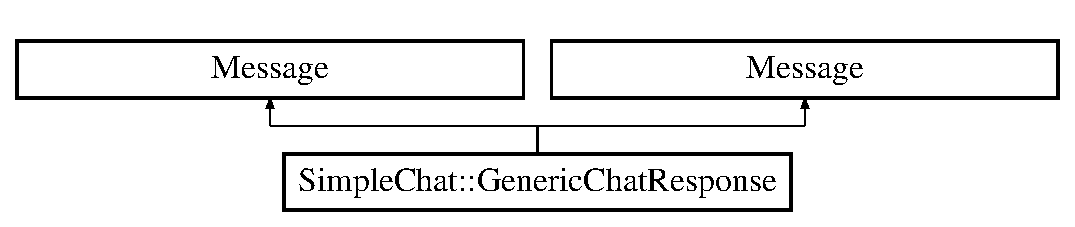
\includegraphics[height=2.000000cm]{classSimpleChat_1_1GenericChatResponse}
\end{center}
\end{figure}
\subsection*{Public Member Functions}
\begin{DoxyCompactItemize}
\item 
\hypertarget{classSimpleChat_1_1GenericChatResponse_a8c213083a5187cc88248f73f4b9caa32}{{\bfseries Generic\-Chat\-Response} (const \hyperlink{classSimpleChat_1_1GenericChatResponse}{Generic\-Chat\-Response} \&from)}\label{classSimpleChat_1_1GenericChatResponse_a8c213083a5187cc88248f73f4b9caa32}

\item 
\hypertarget{classSimpleChat_1_1GenericChatResponse_ab7b303384a8be058542514257b823e7a}{\hyperlink{classSimpleChat_1_1GenericChatResponse}{Generic\-Chat\-Response} \& {\bfseries operator=} (const \hyperlink{classSimpleChat_1_1GenericChatResponse}{Generic\-Chat\-Response} \&from)}\label{classSimpleChat_1_1GenericChatResponse_ab7b303384a8be058542514257b823e7a}

\item 
\hypertarget{classSimpleChat_1_1GenericChatResponse_a6b96bcbb3707721c86be7cd8f0141257}{const \\*
\-::google\-::protobuf\-::\-Unknown\-Field\-Set \& {\bfseries unknown\-\_\-fields} () const }\label{classSimpleChat_1_1GenericChatResponse_a6b96bcbb3707721c86be7cd8f0141257}

\item 
\hypertarget{classSimpleChat_1_1GenericChatResponse_ae9b3f178e2c1977419b592d6e34514fb}{inline\-::google\-::protobuf\-::\-Unknown\-Field\-Set $\ast$ {\bfseries mutable\-\_\-unknown\-\_\-fields} ()}\label{classSimpleChat_1_1GenericChatResponse_ae9b3f178e2c1977419b592d6e34514fb}

\item 
\hypertarget{classSimpleChat_1_1GenericChatResponse_aa5291bf3846f40f0b31b3ed7067e2830}{void {\bfseries Swap} (\hyperlink{classSimpleChat_1_1GenericChatResponse}{Generic\-Chat\-Response} $\ast$other)}\label{classSimpleChat_1_1GenericChatResponse_aa5291bf3846f40f0b31b3ed7067e2830}

\item 
\hypertarget{classSimpleChat_1_1GenericChatResponse_a1a738fd772bbba861c3ba4647d80e71f}{\hyperlink{classSimpleChat_1_1GenericChatResponse}{Generic\-Chat\-Response} $\ast$ {\bfseries New} () const }\label{classSimpleChat_1_1GenericChatResponse_a1a738fd772bbba861c3ba4647d80e71f}

\item 
\hypertarget{classSimpleChat_1_1GenericChatResponse_a02271f6d048eb69dd91bcab14f9139b5}{\hyperlink{classSimpleChat_1_1GenericChatResponse}{Generic\-Chat\-Response} $\ast$ {\bfseries New} (\-::google\-::protobuf\-::\-Arena $\ast$arena) const }\label{classSimpleChat_1_1GenericChatResponse_a02271f6d048eb69dd91bcab14f9139b5}

\item 
\hypertarget{classSimpleChat_1_1GenericChatResponse_a9d9883cca317bbe081516a7ca46a516e}{void {\bfseries Copy\-From} (const \-::google\-::protobuf\-::\-Message \&from)}\label{classSimpleChat_1_1GenericChatResponse_a9d9883cca317bbe081516a7ca46a516e}

\item 
\hypertarget{classSimpleChat_1_1GenericChatResponse_a2a8fbf5f7d1166950df9853a7c596c21}{void {\bfseries Merge\-From} (const \-::google\-::protobuf\-::\-Message \&from)}\label{classSimpleChat_1_1GenericChatResponse_a2a8fbf5f7d1166950df9853a7c596c21}

\item 
\hypertarget{classSimpleChat_1_1GenericChatResponse_a0551253c17a771b8cd7bc4ff4a09ff81}{void {\bfseries Copy\-From} (const \hyperlink{classSimpleChat_1_1GenericChatResponse}{Generic\-Chat\-Response} \&from)}\label{classSimpleChat_1_1GenericChatResponse_a0551253c17a771b8cd7bc4ff4a09ff81}

\item 
\hypertarget{classSimpleChat_1_1GenericChatResponse_abe6dadf25acccc233524f6227e2994f0}{void {\bfseries Merge\-From} (const \hyperlink{classSimpleChat_1_1GenericChatResponse}{Generic\-Chat\-Response} \&from)}\label{classSimpleChat_1_1GenericChatResponse_abe6dadf25acccc233524f6227e2994f0}

\item 
\hypertarget{classSimpleChat_1_1GenericChatResponse_afb1f19ffa65529b74e622e291f38d075}{void {\bfseries Clear} ()}\label{classSimpleChat_1_1GenericChatResponse_afb1f19ffa65529b74e622e291f38d075}

\item 
\hypertarget{classSimpleChat_1_1GenericChatResponse_a3d6649eb8abf4d055ffe421273ec07de}{bool {\bfseries Is\-Initialized} () const }\label{classSimpleChat_1_1GenericChatResponse_a3d6649eb8abf4d055ffe421273ec07de}

\item 
\hypertarget{classSimpleChat_1_1GenericChatResponse_ac42eb1e8033396d861bd9b8ff139e5e9}{int {\bfseries Byte\-Size} () const }\label{classSimpleChat_1_1GenericChatResponse_ac42eb1e8033396d861bd9b8ff139e5e9}

\item 
\hypertarget{classSimpleChat_1_1GenericChatResponse_a1e7991aa5686baf276236982fd7dfd56}{bool {\bfseries Merge\-Partial\-From\-Coded\-Stream} (\-::google\-::protobuf\-::io\-::\-Coded\-Input\-Stream $\ast$input)}\label{classSimpleChat_1_1GenericChatResponse_a1e7991aa5686baf276236982fd7dfd56}

\item 
\hypertarget{classSimpleChat_1_1GenericChatResponse_a5bbfac4cb84098769417c5ebf7b8a6a5}{void {\bfseries Serialize\-With\-Cached\-Sizes} (\-::google\-::protobuf\-::io\-::\-Coded\-Output\-Stream $\ast$output) const }\label{classSimpleChat_1_1GenericChatResponse_a5bbfac4cb84098769417c5ebf7b8a6a5}

\item 
\hypertarget{classSimpleChat_1_1GenericChatResponse_a410b38778b5e7cd91400c8d088211427}{\-::google\-::protobuf\-::uint8 $\ast$ {\bfseries Serialize\-With\-Cached\-Sizes\-To\-Array} (\-::google\-::protobuf\-::uint8 $\ast$output) const }\label{classSimpleChat_1_1GenericChatResponse_a410b38778b5e7cd91400c8d088211427}

\item 
\hypertarget{classSimpleChat_1_1GenericChatResponse_a692cbfe2c4b4a38b6dd19b63748aaa76}{int {\bfseries Get\-Cached\-Size} () const }\label{classSimpleChat_1_1GenericChatResponse_a692cbfe2c4b4a38b6dd19b63748aaa76}

\item 
\hypertarget{classSimpleChat_1_1GenericChatResponse_adf50813e8fe7ae8b49e0447b5a63931e}{\-::google\-::protobuf\-::\-Metadata {\bfseries Get\-Metadata} () const }\label{classSimpleChat_1_1GenericChatResponse_adf50813e8fe7ae8b49e0447b5a63931e}

\item 
\hypertarget{classSimpleChat_1_1GenericChatResponse_a3d47070052c5365722bd691ac9765934}{bool {\bfseries has\-\_\-success} () const }\label{classSimpleChat_1_1GenericChatResponse_a3d47070052c5365722bd691ac9765934}

\item 
\hypertarget{classSimpleChat_1_1GenericChatResponse_a6454d5a3dbf1a65e3278fb92dd7e8793}{void {\bfseries clear\-\_\-success} ()}\label{classSimpleChat_1_1GenericChatResponse_a6454d5a3dbf1a65e3278fb92dd7e8793}

\item 
\hypertarget{classSimpleChat_1_1GenericChatResponse_a1b8a7a5eb65cc06bc202e56b28624444}{bool {\bfseries success} () const }\label{classSimpleChat_1_1GenericChatResponse_a1b8a7a5eb65cc06bc202e56b28624444}

\item 
\hypertarget{classSimpleChat_1_1GenericChatResponse_a616a4c030969288563569cc0676ae7c3}{void {\bfseries set\-\_\-success} (bool value)}\label{classSimpleChat_1_1GenericChatResponse_a616a4c030969288563569cc0676ae7c3}

\item 
\hypertarget{classSimpleChat_1_1GenericChatResponse_a8e0cfcd074450aff7e281e41b43a5d7c}{bool {\bfseries has\-\_\-message} () const }\label{classSimpleChat_1_1GenericChatResponse_a8e0cfcd074450aff7e281e41b43a5d7c}

\item 
\hypertarget{classSimpleChat_1_1GenericChatResponse_add65fb031dd10bbc3e0a1bd102ae5346}{void {\bfseries clear\-\_\-message} ()}\label{classSimpleChat_1_1GenericChatResponse_add65fb031dd10bbc3e0a1bd102ae5346}

\item 
\hypertarget{classSimpleChat_1_1GenericChatResponse_a3d25be251d3df608720630fb09b96b57}{const \-::std\-::string \& {\bfseries message} () const }\label{classSimpleChat_1_1GenericChatResponse_a3d25be251d3df608720630fb09b96b57}

\item 
\hypertarget{classSimpleChat_1_1GenericChatResponse_a9aaf46c1517c9ba82234d1c9d0a89bfc}{void {\bfseries set\-\_\-message} (const \-::std\-::string \&value)}\label{classSimpleChat_1_1GenericChatResponse_a9aaf46c1517c9ba82234d1c9d0a89bfc}

\item 
\hypertarget{classSimpleChat_1_1GenericChatResponse_a13db499f10cc62f34730ae82a4889d18}{void {\bfseries set\-\_\-message} (const char $\ast$value)}\label{classSimpleChat_1_1GenericChatResponse_a13db499f10cc62f34730ae82a4889d18}

\item 
\hypertarget{classSimpleChat_1_1GenericChatResponse_a04ad5f0c624490b5d08e3aba400fd8b3}{void {\bfseries set\-\_\-message} (const char $\ast$value, size\-\_\-t size)}\label{classSimpleChat_1_1GenericChatResponse_a04ad5f0c624490b5d08e3aba400fd8b3}

\item 
\hypertarget{classSimpleChat_1_1GenericChatResponse_a026780cc0beb230f89a357b3be290eb5}{\-::std\-::string $\ast$ {\bfseries mutable\-\_\-message} ()}\label{classSimpleChat_1_1GenericChatResponse_a026780cc0beb230f89a357b3be290eb5}

\item 
\hypertarget{classSimpleChat_1_1GenericChatResponse_a9085f0f820c7b164630799b74452ad3f}{\-::std\-::string $\ast$ {\bfseries release\-\_\-message} ()}\label{classSimpleChat_1_1GenericChatResponse_a9085f0f820c7b164630799b74452ad3f}

\item 
\hypertarget{classSimpleChat_1_1GenericChatResponse_a537a1746cc407ed748b06e97d3517a31}{void {\bfseries set\-\_\-allocated\-\_\-message} (\-::std\-::string $\ast$message)}\label{classSimpleChat_1_1GenericChatResponse_a537a1746cc407ed748b06e97d3517a31}

\item 
\hypertarget{classSimpleChat_1_1GenericChatResponse_a8c213083a5187cc88248f73f4b9caa32}{{\bfseries Generic\-Chat\-Response} (const \hyperlink{classSimpleChat_1_1GenericChatResponse}{Generic\-Chat\-Response} \&from)}\label{classSimpleChat_1_1GenericChatResponse_a8c213083a5187cc88248f73f4b9caa32}

\item 
\hypertarget{classSimpleChat_1_1GenericChatResponse_ab7b303384a8be058542514257b823e7a}{\hyperlink{classSimpleChat_1_1GenericChatResponse}{Generic\-Chat\-Response} \& {\bfseries operator=} (const \hyperlink{classSimpleChat_1_1GenericChatResponse}{Generic\-Chat\-Response} \&from)}\label{classSimpleChat_1_1GenericChatResponse_ab7b303384a8be058542514257b823e7a}

\item 
\hypertarget{classSimpleChat_1_1GenericChatResponse_a6b96bcbb3707721c86be7cd8f0141257}{const \\*
\-::google\-::protobuf\-::\-Unknown\-Field\-Set \& {\bfseries unknown\-\_\-fields} () const }\label{classSimpleChat_1_1GenericChatResponse_a6b96bcbb3707721c86be7cd8f0141257}

\item 
\hypertarget{classSimpleChat_1_1GenericChatResponse_ae9b3f178e2c1977419b592d6e34514fb}{inline\-::google\-::protobuf\-::\-Unknown\-Field\-Set $\ast$ {\bfseries mutable\-\_\-unknown\-\_\-fields} ()}\label{classSimpleChat_1_1GenericChatResponse_ae9b3f178e2c1977419b592d6e34514fb}

\item 
\hypertarget{classSimpleChat_1_1GenericChatResponse_aa5291bf3846f40f0b31b3ed7067e2830}{void {\bfseries Swap} (\hyperlink{classSimpleChat_1_1GenericChatResponse}{Generic\-Chat\-Response} $\ast$other)}\label{classSimpleChat_1_1GenericChatResponse_aa5291bf3846f40f0b31b3ed7067e2830}

\item 
\hypertarget{classSimpleChat_1_1GenericChatResponse_a1a738fd772bbba861c3ba4647d80e71f}{\hyperlink{classSimpleChat_1_1GenericChatResponse}{Generic\-Chat\-Response} $\ast$ {\bfseries New} () const }\label{classSimpleChat_1_1GenericChatResponse_a1a738fd772bbba861c3ba4647d80e71f}

\item 
\hypertarget{classSimpleChat_1_1GenericChatResponse_a02271f6d048eb69dd91bcab14f9139b5}{\hyperlink{classSimpleChat_1_1GenericChatResponse}{Generic\-Chat\-Response} $\ast$ {\bfseries New} (\-::google\-::protobuf\-::\-Arena $\ast$arena) const }\label{classSimpleChat_1_1GenericChatResponse_a02271f6d048eb69dd91bcab14f9139b5}

\item 
\hypertarget{classSimpleChat_1_1GenericChatResponse_a9d9883cca317bbe081516a7ca46a516e}{void {\bfseries Copy\-From} (const \-::google\-::protobuf\-::\-Message \&from)}\label{classSimpleChat_1_1GenericChatResponse_a9d9883cca317bbe081516a7ca46a516e}

\item 
\hypertarget{classSimpleChat_1_1GenericChatResponse_a2a8fbf5f7d1166950df9853a7c596c21}{void {\bfseries Merge\-From} (const \-::google\-::protobuf\-::\-Message \&from)}\label{classSimpleChat_1_1GenericChatResponse_a2a8fbf5f7d1166950df9853a7c596c21}

\item 
\hypertarget{classSimpleChat_1_1GenericChatResponse_a0551253c17a771b8cd7bc4ff4a09ff81}{void {\bfseries Copy\-From} (const \hyperlink{classSimpleChat_1_1GenericChatResponse}{Generic\-Chat\-Response} \&from)}\label{classSimpleChat_1_1GenericChatResponse_a0551253c17a771b8cd7bc4ff4a09ff81}

\item 
\hypertarget{classSimpleChat_1_1GenericChatResponse_abe6dadf25acccc233524f6227e2994f0}{void {\bfseries Merge\-From} (const \hyperlink{classSimpleChat_1_1GenericChatResponse}{Generic\-Chat\-Response} \&from)}\label{classSimpleChat_1_1GenericChatResponse_abe6dadf25acccc233524f6227e2994f0}

\item 
\hypertarget{classSimpleChat_1_1GenericChatResponse_afb1f19ffa65529b74e622e291f38d075}{void {\bfseries Clear} ()}\label{classSimpleChat_1_1GenericChatResponse_afb1f19ffa65529b74e622e291f38d075}

\item 
\hypertarget{classSimpleChat_1_1GenericChatResponse_a3d6649eb8abf4d055ffe421273ec07de}{bool {\bfseries Is\-Initialized} () const }\label{classSimpleChat_1_1GenericChatResponse_a3d6649eb8abf4d055ffe421273ec07de}

\item 
\hypertarget{classSimpleChat_1_1GenericChatResponse_ac42eb1e8033396d861bd9b8ff139e5e9}{int {\bfseries Byte\-Size} () const }\label{classSimpleChat_1_1GenericChatResponse_ac42eb1e8033396d861bd9b8ff139e5e9}

\item 
\hypertarget{classSimpleChat_1_1GenericChatResponse_a1e7991aa5686baf276236982fd7dfd56}{bool {\bfseries Merge\-Partial\-From\-Coded\-Stream} (\-::google\-::protobuf\-::io\-::\-Coded\-Input\-Stream $\ast$input)}\label{classSimpleChat_1_1GenericChatResponse_a1e7991aa5686baf276236982fd7dfd56}

\item 
\hypertarget{classSimpleChat_1_1GenericChatResponse_a5bbfac4cb84098769417c5ebf7b8a6a5}{void {\bfseries Serialize\-With\-Cached\-Sizes} (\-::google\-::protobuf\-::io\-::\-Coded\-Output\-Stream $\ast$output) const }\label{classSimpleChat_1_1GenericChatResponse_a5bbfac4cb84098769417c5ebf7b8a6a5}

\item 
\hypertarget{classSimpleChat_1_1GenericChatResponse_a410b38778b5e7cd91400c8d088211427}{\-::google\-::protobuf\-::uint8 $\ast$ {\bfseries Serialize\-With\-Cached\-Sizes\-To\-Array} (\-::google\-::protobuf\-::uint8 $\ast$output) const }\label{classSimpleChat_1_1GenericChatResponse_a410b38778b5e7cd91400c8d088211427}

\item 
\hypertarget{classSimpleChat_1_1GenericChatResponse_a692cbfe2c4b4a38b6dd19b63748aaa76}{int {\bfseries Get\-Cached\-Size} () const }\label{classSimpleChat_1_1GenericChatResponse_a692cbfe2c4b4a38b6dd19b63748aaa76}

\item 
\hypertarget{classSimpleChat_1_1GenericChatResponse_adf50813e8fe7ae8b49e0447b5a63931e}{\-::google\-::protobuf\-::\-Metadata {\bfseries Get\-Metadata} () const }\label{classSimpleChat_1_1GenericChatResponse_adf50813e8fe7ae8b49e0447b5a63931e}

\item 
\hypertarget{classSimpleChat_1_1GenericChatResponse_a3d47070052c5365722bd691ac9765934}{bool {\bfseries has\-\_\-success} () const }\label{classSimpleChat_1_1GenericChatResponse_a3d47070052c5365722bd691ac9765934}

\item 
\hypertarget{classSimpleChat_1_1GenericChatResponse_a6454d5a3dbf1a65e3278fb92dd7e8793}{void {\bfseries clear\-\_\-success} ()}\label{classSimpleChat_1_1GenericChatResponse_a6454d5a3dbf1a65e3278fb92dd7e8793}

\item 
\hypertarget{classSimpleChat_1_1GenericChatResponse_a1b8a7a5eb65cc06bc202e56b28624444}{bool {\bfseries success} () const }\label{classSimpleChat_1_1GenericChatResponse_a1b8a7a5eb65cc06bc202e56b28624444}

\item 
\hypertarget{classSimpleChat_1_1GenericChatResponse_a616a4c030969288563569cc0676ae7c3}{void {\bfseries set\-\_\-success} (bool value)}\label{classSimpleChat_1_1GenericChatResponse_a616a4c030969288563569cc0676ae7c3}

\item 
\hypertarget{classSimpleChat_1_1GenericChatResponse_a8e0cfcd074450aff7e281e41b43a5d7c}{bool {\bfseries has\-\_\-message} () const }\label{classSimpleChat_1_1GenericChatResponse_a8e0cfcd074450aff7e281e41b43a5d7c}

\item 
\hypertarget{classSimpleChat_1_1GenericChatResponse_add65fb031dd10bbc3e0a1bd102ae5346}{void {\bfseries clear\-\_\-message} ()}\label{classSimpleChat_1_1GenericChatResponse_add65fb031dd10bbc3e0a1bd102ae5346}

\item 
\hypertarget{classSimpleChat_1_1GenericChatResponse_ae03944157c32ce713a45413d825408e3}{const \-::std\-::string \& {\bfseries message} () const }\label{classSimpleChat_1_1GenericChatResponse_ae03944157c32ce713a45413d825408e3}

\item 
\hypertarget{classSimpleChat_1_1GenericChatResponse_a9aaf46c1517c9ba82234d1c9d0a89bfc}{void {\bfseries set\-\_\-message} (const \-::std\-::string \&value)}\label{classSimpleChat_1_1GenericChatResponse_a9aaf46c1517c9ba82234d1c9d0a89bfc}

\item 
\hypertarget{classSimpleChat_1_1GenericChatResponse_a13db499f10cc62f34730ae82a4889d18}{void {\bfseries set\-\_\-message} (const char $\ast$value)}\label{classSimpleChat_1_1GenericChatResponse_a13db499f10cc62f34730ae82a4889d18}

\item 
\hypertarget{classSimpleChat_1_1GenericChatResponse_a04ad5f0c624490b5d08e3aba400fd8b3}{void {\bfseries set\-\_\-message} (const char $\ast$value, size\-\_\-t size)}\label{classSimpleChat_1_1GenericChatResponse_a04ad5f0c624490b5d08e3aba400fd8b3}

\item 
\hypertarget{classSimpleChat_1_1GenericChatResponse_aa0bef76137dfe02e0b414cc5081477fe}{\-::std\-::string $\ast$ {\bfseries mutable\-\_\-message} ()}\label{classSimpleChat_1_1GenericChatResponse_aa0bef76137dfe02e0b414cc5081477fe}

\item 
\hypertarget{classSimpleChat_1_1GenericChatResponse_a10c8689675f47843a75acbcc4613c44e}{\-::std\-::string $\ast$ {\bfseries release\-\_\-message} ()}\label{classSimpleChat_1_1GenericChatResponse_a10c8689675f47843a75acbcc4613c44e}

\item 
\hypertarget{classSimpleChat_1_1GenericChatResponse_a537a1746cc407ed748b06e97d3517a31}{void {\bfseries set\-\_\-allocated\-\_\-message} (\-::std\-::string $\ast$message)}\label{classSimpleChat_1_1GenericChatResponse_a537a1746cc407ed748b06e97d3517a31}

\end{DoxyCompactItemize}
\subsection*{Static Public Member Functions}
\begin{DoxyCompactItemize}
\item 
\hypertarget{classSimpleChat_1_1GenericChatResponse_a239ac446ce60ca453359b12bb5309e2a}{static const \\*
\-::google\-::protobuf\-::\-Descriptor $\ast$ {\bfseries descriptor} ()}\label{classSimpleChat_1_1GenericChatResponse_a239ac446ce60ca453359b12bb5309e2a}

\item 
\hypertarget{classSimpleChat_1_1GenericChatResponse_a05778077bddee03fd2e2feba394cb50c}{static const \hyperlink{classSimpleChat_1_1GenericChatResponse}{Generic\-Chat\-Response} \& {\bfseries default\-\_\-instance} ()}\label{classSimpleChat_1_1GenericChatResponse_a05778077bddee03fd2e2feba394cb50c}

\item 
\hypertarget{classSimpleChat_1_1GenericChatResponse_a239ac446ce60ca453359b12bb5309e2a}{static const \\*
\-::google\-::protobuf\-::\-Descriptor $\ast$ {\bfseries descriptor} ()}\label{classSimpleChat_1_1GenericChatResponse_a239ac446ce60ca453359b12bb5309e2a}

\item 
\hypertarget{classSimpleChat_1_1GenericChatResponse_a05778077bddee03fd2e2feba394cb50c}{static const \hyperlink{classSimpleChat_1_1GenericChatResponse}{Generic\-Chat\-Response} \& {\bfseries default\-\_\-instance} ()}\label{classSimpleChat_1_1GenericChatResponse_a05778077bddee03fd2e2feba394cb50c}

\end{DoxyCompactItemize}
\subsection*{Static Public Attributes}
\begin{DoxyCompactItemize}
\item 
\hypertarget{classSimpleChat_1_1GenericChatResponse_a473ca246e05ffceebe6b40435446443b}{static const int {\bfseries k\-Success\-Field\-Number} = 1}\label{classSimpleChat_1_1GenericChatResponse_a473ca246e05ffceebe6b40435446443b}

\item 
\hypertarget{classSimpleChat_1_1GenericChatResponse_a80c3f6d2ea5d4ac0958848671084fb1f}{static const int {\bfseries k\-Message\-Field\-Number} = 2}\label{classSimpleChat_1_1GenericChatResponse_a80c3f6d2ea5d4ac0958848671084fb1f}

\end{DoxyCompactItemize}
\subsection*{Friends}
\begin{DoxyCompactItemize}
\item 
\hypertarget{classSimpleChat_1_1GenericChatResponse_ab0d9593aa41361f04ab91f917ef9ec0e}{void {\bfseries protobuf\-\_\-\-Add\-Desc\-\_\-\-Chat\-Message\-\_\-2eproto} ()}\label{classSimpleChat_1_1GenericChatResponse_ab0d9593aa41361f04ab91f917ef9ec0e}

\item 
\hypertarget{classSimpleChat_1_1GenericChatResponse_a4ca7b2c64786782406ca69f6ba39ccb2}{void {\bfseries protobuf\-\_\-\-Assign\-Desc\-\_\-\-Chat\-Message\-\_\-2eproto} ()}\label{classSimpleChat_1_1GenericChatResponse_a4ca7b2c64786782406ca69f6ba39ccb2}

\item 
\hypertarget{classSimpleChat_1_1GenericChatResponse_a78726b79d52a130a50d7670a5c0238fc}{void {\bfseries protobuf\-\_\-\-Shutdown\-File\-\_\-\-Chat\-Message\-\_\-2eproto} ()}\label{classSimpleChat_1_1GenericChatResponse_a78726b79d52a130a50d7670a5c0238fc}

\item 
\hypertarget{classSimpleChat_1_1GenericChatResponse_ab0d9593aa41361f04ab91f917ef9ec0e}{void {\bfseries protobuf\-\_\-\-Add\-Desc\-\_\-\-Chat\-Message\-\_\-2eproto} ()}\label{classSimpleChat_1_1GenericChatResponse_ab0d9593aa41361f04ab91f917ef9ec0e}

\item 
\hypertarget{classSimpleChat_1_1GenericChatResponse_a4ca7b2c64786782406ca69f6ba39ccb2}{void {\bfseries protobuf\-\_\-\-Assign\-Desc\-\_\-\-Chat\-Message\-\_\-2eproto} ()}\label{classSimpleChat_1_1GenericChatResponse_a4ca7b2c64786782406ca69f6ba39ccb2}

\item 
\hypertarget{classSimpleChat_1_1GenericChatResponse_a78726b79d52a130a50d7670a5c0238fc}{void {\bfseries protobuf\-\_\-\-Shutdown\-File\-\_\-\-Chat\-Message\-\_\-2eproto} ()}\label{classSimpleChat_1_1GenericChatResponse_a78726b79d52a130a50d7670a5c0238fc}

\end{DoxyCompactItemize}


The documentation for this class was generated from the following file\-:\begin{DoxyCompactItemize}
\item 
chatlib/proto/Chat\-Message.\-pb.\-h\end{DoxyCompactItemize}

\hypertarget{structgoogle_1_1protobuf_1_1is__proto__enum_3_01_1_1SimpleChat_1_1CommandType_01_4}{\section{google\-:\-:protobuf\-:\-:is\-\_\-proto\-\_\-enum$<$ \-:\-:Simple\-Chat\-:\-:Command\-Type $>$ Struct Template Reference}
\label{structgoogle_1_1protobuf_1_1is__proto__enum_3_01_1_1SimpleChat_1_1CommandType_01_4}\index{google\-::protobuf\-::is\-\_\-proto\-\_\-enum$<$ \-::\-Simple\-Chat\-::\-Command\-Type $>$@{google\-::protobuf\-::is\-\_\-proto\-\_\-enum$<$ \-::\-Simple\-Chat\-::\-Command\-Type $>$}}
}
Inheritance diagram for google\-:\-:protobuf\-:\-:is\-\_\-proto\-\_\-enum$<$ \-:\-:Simple\-Chat\-:\-:Command\-Type $>$\-:\begin{figure}[H]
\begin{center}
\leavevmode
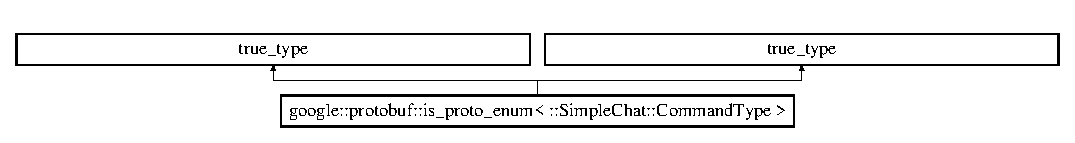
\includegraphics[height=1.469816cm]{structgoogle_1_1protobuf_1_1is__proto__enum_3_01_1_1SimpleChat_1_1CommandType_01_4}
\end{center}
\end{figure}


The documentation for this struct was generated from the following file\-:\begin{DoxyCompactItemize}
\item 
chatlib/proto/Chat\-Message.\-pb.\-h\end{DoxyCompactItemize}

\hypertarget{structgoogle_1_1protobuf_1_1is__proto__enum_3_01_1_1SimpleChat_1_1NetworkMessageType_01_4}{\section{google\-:\-:protobuf\-:\-:is\-\_\-proto\-\_\-enum$<$ \-:\-:Simple\-Chat\-:\-:Network\-Message\-Type $>$ Struct Template Reference}
\label{structgoogle_1_1protobuf_1_1is__proto__enum_3_01_1_1SimpleChat_1_1NetworkMessageType_01_4}\index{google\-::protobuf\-::is\-\_\-proto\-\_\-enum$<$ \-::\-Simple\-Chat\-::\-Network\-Message\-Type $>$@{google\-::protobuf\-::is\-\_\-proto\-\_\-enum$<$ \-::\-Simple\-Chat\-::\-Network\-Message\-Type $>$}}
}
Inheritance diagram for google\-:\-:protobuf\-:\-:is\-\_\-proto\-\_\-enum$<$ \-:\-:Simple\-Chat\-:\-:Network\-Message\-Type $>$\-:\begin{figure}[H]
\begin{center}
\leavevmode
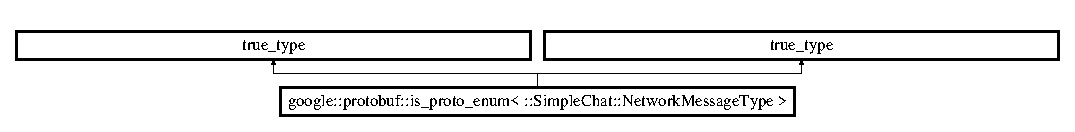
\includegraphics[height=1.323877cm]{structgoogle_1_1protobuf_1_1is__proto__enum_3_01_1_1SimpleChat_1_1NetworkMessageType_01_4}
\end{center}
\end{figure}


The documentation for this struct was generated from the following file\-:\begin{DoxyCompactItemize}
\item 
chatlib/proto/Network\-Message.\-pb.\-h\end{DoxyCompactItemize}

\hypertarget{structgoogle_1_1protobuf_1_1is__proto__enum_3_01_1_1SimpleChat_1_1UserAction_01_4}{\section{google\-:\-:protobuf\-:\-:is\-\_\-proto\-\_\-enum$<$ \-:\-:Simple\-Chat\-:\-:User\-Action $>$ Struct Template Reference}
\label{structgoogle_1_1protobuf_1_1is__proto__enum_3_01_1_1SimpleChat_1_1UserAction_01_4}\index{google\-::protobuf\-::is\-\_\-proto\-\_\-enum$<$ \-::\-Simple\-Chat\-::\-User\-Action $>$@{google\-::protobuf\-::is\-\_\-proto\-\_\-enum$<$ \-::\-Simple\-Chat\-::\-User\-Action $>$}}
}
Inheritance diagram for google\-:\-:protobuf\-:\-:is\-\_\-proto\-\_\-enum$<$ \-:\-:Simple\-Chat\-:\-:User\-Action $>$\-:\begin{figure}[H]
\begin{center}
\leavevmode
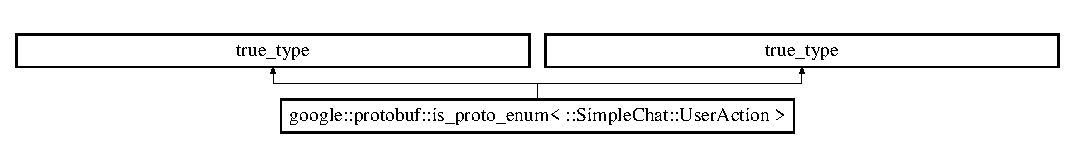
\includegraphics[height=1.555556cm]{structgoogle_1_1protobuf_1_1is__proto__enum_3_01_1_1SimpleChat_1_1UserAction_01_4}
\end{center}
\end{figure}


The documentation for this struct was generated from the following file\-:\begin{DoxyCompactItemize}
\item 
chatlib/proto/User.\-pb.\-h\end{DoxyCompactItemize}

\hypertarget{structgoogle_1_1protobuf_1_1is__proto__enum_3_01_1_1SimpleChat_1_1UserPresence_01_4}{\section{google\-:\-:protobuf\-:\-:is\-\_\-proto\-\_\-enum$<$ \-:\-:Simple\-Chat\-:\-:User\-Presence $>$ Struct Template Reference}
\label{structgoogle_1_1protobuf_1_1is__proto__enum_3_01_1_1SimpleChat_1_1UserPresence_01_4}\index{google\-::protobuf\-::is\-\_\-proto\-\_\-enum$<$ \-::\-Simple\-Chat\-::\-User\-Presence $>$@{google\-::protobuf\-::is\-\_\-proto\-\_\-enum$<$ \-::\-Simple\-Chat\-::\-User\-Presence $>$}}
}
Inheritance diagram for google\-:\-:protobuf\-:\-:is\-\_\-proto\-\_\-enum$<$ \-:\-:Simple\-Chat\-:\-:User\-Presence $>$\-:\begin{figure}[H]
\begin{center}
\leavevmode
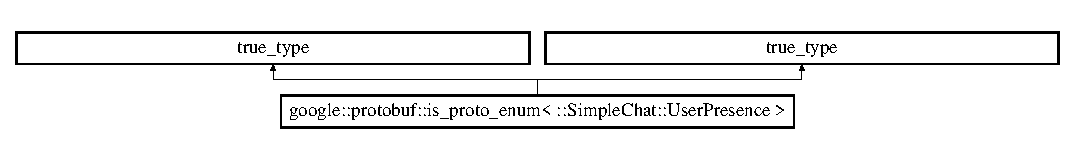
\includegraphics[height=1.481482cm]{structgoogle_1_1protobuf_1_1is__proto__enum_3_01_1_1SimpleChat_1_1UserPresence_01_4}
\end{center}
\end{figure}


The documentation for this struct was generated from the following file\-:\begin{DoxyCompactItemize}
\item 
chatlib/proto/User.\-pb.\-h\end{DoxyCompactItemize}

\hypertarget{structgoogle_1_1protobuf_1_1is__proto__enum_3_01_1_1SimpleChat_1_1UserStatus_01_4}{\section{google\-:\-:protobuf\-:\-:is\-\_\-proto\-\_\-enum$<$ \-:\-:Simple\-Chat\-:\-:User\-Status $>$ Struct Template Reference}
\label{structgoogle_1_1protobuf_1_1is__proto__enum_3_01_1_1SimpleChat_1_1UserStatus_01_4}\index{google\-::protobuf\-::is\-\_\-proto\-\_\-enum$<$ \-::\-Simple\-Chat\-::\-User\-Status $>$@{google\-::protobuf\-::is\-\_\-proto\-\_\-enum$<$ \-::\-Simple\-Chat\-::\-User\-Status $>$}}
}
Inheritance diagram for google\-:\-:protobuf\-:\-:is\-\_\-proto\-\_\-enum$<$ \-:\-:Simple\-Chat\-:\-:User\-Status $>$\-:\begin{figure}[H]
\begin{center}
\leavevmode
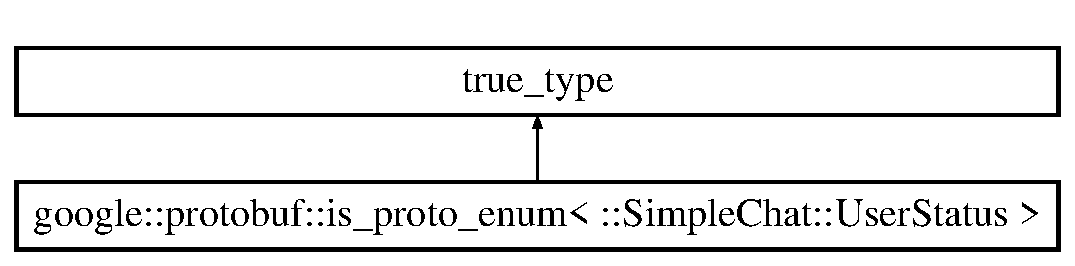
\includegraphics[height=2.000000cm]{structgoogle_1_1protobuf_1_1is__proto__enum_3_01_1_1SimpleChat_1_1UserStatus_01_4}
\end{center}
\end{figure}


The documentation for this struct was generated from the following file\-:\begin{DoxyCompactItemize}
\item 
shared/proto/User.\-pb.\-h\end{DoxyCompactItemize}

\hypertarget{classSimpleChat_1_1KickChatCommand}{\section{Simple\-Chat\-:\-:Kick\-Chat\-Command Class Reference}
\label{classSimpleChat_1_1KickChatCommand}\index{Simple\-Chat\-::\-Kick\-Chat\-Command@{Simple\-Chat\-::\-Kick\-Chat\-Command}}
}
Inheritance diagram for Simple\-Chat\-:\-:Kick\-Chat\-Command\-:\begin{figure}[H]
\begin{center}
\leavevmode
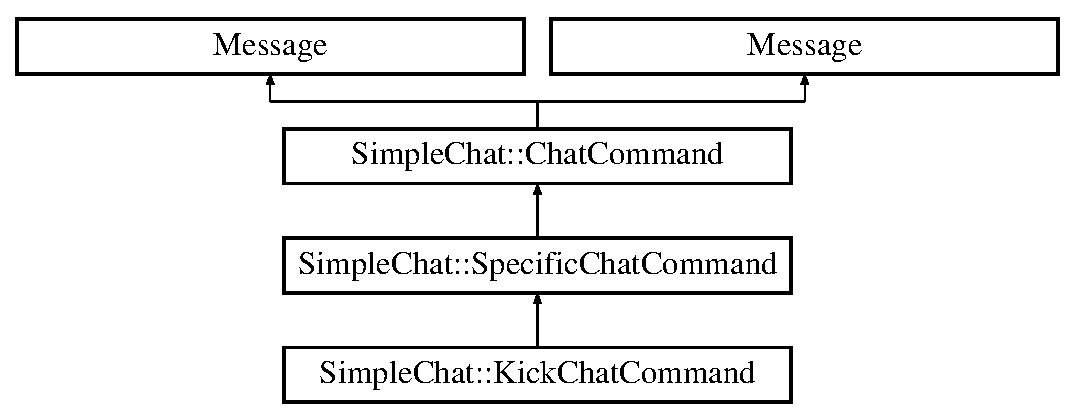
\includegraphics[height=4.000000cm]{classSimpleChat_1_1KickChatCommand}
\end{center}
\end{figure}
\subsection*{Public Member Functions}
\begin{DoxyCompactItemize}
\item 
virtual void \hyperlink{classSimpleChat_1_1KickChatCommand_ab2e0cb6f03475b4636c487f0cd997308}{insert\-Data} (const std\-::vector$<$ std\-::string $>$ \&arguments) override
\end{DoxyCompactItemize}
\subsection*{Additional Inherited Members}


\subsection{Member Function Documentation}
\hypertarget{classSimpleChat_1_1KickChatCommand_ab2e0cb6f03475b4636c487f0cd997308}{\index{Simple\-Chat\-::\-Kick\-Chat\-Command@{Simple\-Chat\-::\-Kick\-Chat\-Command}!insert\-Data@{insert\-Data}}
\index{insert\-Data@{insert\-Data}!SimpleChat::KickChatCommand@{Simple\-Chat\-::\-Kick\-Chat\-Command}}
\subsubsection[{insert\-Data}]{\setlength{\rightskip}{0pt plus 5cm}void Simple\-Chat\-::\-Kick\-Chat\-Command\-::insert\-Data (
\begin{DoxyParamCaption}
\item[{const std\-::vector$<$ std\-::string $>$ \&}]{arguments}
\end{DoxyParamCaption}
)\hspace{0.3cm}{\ttfamily [override]}, {\ttfamily [virtual]}}}\label{classSimpleChat_1_1KickChatCommand_ab2e0cb6f03475b4636c487f0cd997308}
argument is a name 

Implements \hyperlink{classSimpleChat_1_1SpecificChatCommand}{Simple\-Chat\-::\-Specific\-Chat\-Command}.



The documentation for this class was generated from the following files\-:\begin{DoxyCompactItemize}
\item 
chatlib/chat/commands/Kick\-Chat\-Command.\-h\item 
chatlib/chat/commands/Kick\-Chat\-Command.\-cpp\end{DoxyCompactItemize}

\hypertarget{classSimpleChat_1_1LoginDialog}{\section{Simple\-Chat\-:\-:Login\-Dialog Class Reference}
\label{classSimpleChat_1_1LoginDialog}\index{Simple\-Chat\-::\-Login\-Dialog@{Simple\-Chat\-::\-Login\-Dialog}}
}
Inheritance diagram for Simple\-Chat\-:\-:Login\-Dialog\-:\begin{figure}[H]
\begin{center}
\leavevmode
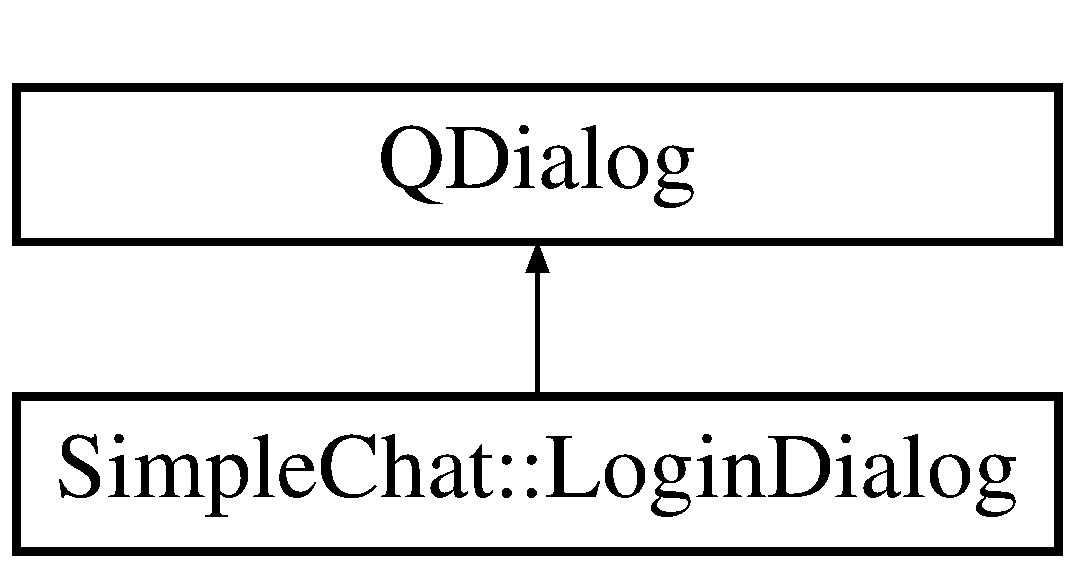
\includegraphics[height=2.000000cm]{classSimpleChat_1_1LoginDialog}
\end{center}
\end{figure}
\subsection*{Signals}
\begin{DoxyCompactItemize}
\item 
\hypertarget{classSimpleChat_1_1LoginDialog_a8fc7aa0dc471e1cde705bb74daadd3b5}{void {\bfseries login\-Signal} (const Q\-String \&address, quint16 port, const Q\-String \&name)}\label{classSimpleChat_1_1LoginDialog_a8fc7aa0dc471e1cde705bb74daadd3b5}

\end{DoxyCompactItemize}
\subsection*{Public Member Functions}
\begin{DoxyCompactItemize}
\item 
\hypertarget{classSimpleChat_1_1LoginDialog_a513ec2c3e7b82b47d71dc10ac1b73179}{{\bfseries Login\-Dialog} (Q\-Widget $\ast$parent=nullptr)}\label{classSimpleChat_1_1LoginDialog_a513ec2c3e7b82b47d71dc10ac1b73179}

\item 
\hypertarget{classSimpleChat_1_1LoginDialog_a254731e112e817fa66c323ef227a7ba3}{void {\bfseries setup\-Dialog} ()}\label{classSimpleChat_1_1LoginDialog_a254731e112e817fa66c323ef227a7ba3}

\item 
\hypertarget{classSimpleChat_1_1LoginDialog_ae53fd7b92225a512632d8836e35baad3}{void {\bfseries set\-Enable\-Login} (bool enabled) const }\label{classSimpleChat_1_1LoginDialog_ae53fd7b92225a512632d8836e35baad3}

\end{DoxyCompactItemize}


The documentation for this class was generated from the following files\-:\begin{DoxyCompactItemize}
\item 
client/dialog/Login\-Dialog.\-h\item 
client/dialog/Login\-Dialog.\-cpp\item 
client/moc\-\_\-\-Login\-Dialog.\-cpp\end{DoxyCompactItemize}

\hypertarget{classSimpleChat_1_1Message}{\section{Simple\-Chat\-:\-:Message$<$ Message\-Type, typename $>$ Class Template Reference}
\label{classSimpleChat_1_1Message}\index{Simple\-Chat\-::\-Message$<$ Message\-Type, typename $>$@{Simple\-Chat\-::\-Message$<$ Message\-Type, typename $>$}}
}
Inheritance diagram for Simple\-Chat\-:\-:Message$<$ Message\-Type, typename $>$\-:\begin{figure}[H]
\begin{center}
\leavevmode
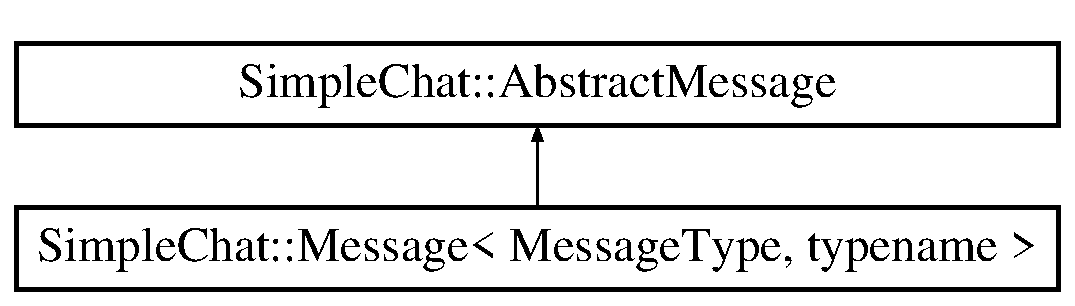
\includegraphics[height=2.000000cm]{classSimpleChat_1_1Message}
\end{center}
\end{figure}
\subsection*{Public Member Functions}
\begin{DoxyCompactItemize}
\item 
\hypertarget{classSimpleChat_1_1Message_a5e589f4b47b48c6c2a57395e7da5a1da}{{\bfseries Message} (std\-::unique\-\_\-ptr$<$ Message\-Type $>$ message, int type)}\label{classSimpleChat_1_1Message_a5e589f4b47b48c6c2a57395e7da5a1da}

\item 
\hypertarget{classSimpleChat_1_1Message_a10d69aeec672948394683cc3b3943551}{std\-::string {\bfseries serialize} () override}\label{classSimpleChat_1_1Message_a10d69aeec672948394683cc3b3943551}

\item 
\hypertarget{classSimpleChat_1_1Message_a26ee452950cb78108a2d3f4d2c7be436}{virtual int {\bfseries type} () override}\label{classSimpleChat_1_1Message_a26ee452950cb78108a2d3f4d2c7be436}

\item 
\hypertarget{classSimpleChat_1_1Message_abcff4eb636679bc459d40e312f296f52}{virtual bool {\bfseries is\-Initialized} () override}\label{classSimpleChat_1_1Message_abcff4eb636679bc459d40e312f296f52}

\item 
\hypertarget{classSimpleChat_1_1Message_a360640255aa3288041c747840dae975e}{virtual std\-::unique\-\_\-ptr\\*
$<$ \hyperlink{classSimpleChat_1_1AbstractMessage}{Abstract\-Message} $>$ {\bfseries clone} () override}\label{classSimpleChat_1_1Message_a360640255aa3288041c747840dae975e}

\end{DoxyCompactItemize}


The documentation for this class was generated from the following file\-:\begin{DoxyCompactItemize}
\item 
chatlib/communication/Message.\-h\end{DoxyCompactItemize}

\hypertarget{classSimpleChat_1_1MessageBuilder}{\section{Simple\-Chat\-:\-:Message\-Builder Class Reference}
\label{classSimpleChat_1_1MessageBuilder}\index{Simple\-Chat\-::\-Message\-Builder@{Simple\-Chat\-::\-Message\-Builder}}
}
\subsection*{Static Public Member Functions}
\begin{DoxyCompactItemize}
\item 
\hypertarget{classSimpleChat_1_1MessageBuilder_a7dec768a4ac3206671a1e77b4516e6c3}{static std\-::unique\-\_\-ptr\\*
$<$ \hyperlink{classSimpleChat_1_1Message}{Message}$<$ \hyperlink{classSimpleChat_1_1UserJoinRequest}{User\-Join\-Request} $>$ $>$ {\bfseries build} (std\-::unique\-\_\-ptr$<$ \hyperlink{classSimpleChat_1_1UserJoinRequest}{User\-Join\-Request} $>$ message)}\label{classSimpleChat_1_1MessageBuilder_a7dec768a4ac3206671a1e77b4516e6c3}

\item 
\hypertarget{classSimpleChat_1_1MessageBuilder_ad0c528702aba9f95737341a313a5b7c8}{static std\-::unique\-\_\-ptr\\*
$<$ \hyperlink{classSimpleChat_1_1Message}{Message}$<$ \hyperlink{classSimpleChat_1_1UserJoinResponse}{User\-Join\-Response} $>$ $>$ {\bfseries build} (std\-::unique\-\_\-ptr$<$ \hyperlink{classSimpleChat_1_1UserJoinResponse}{User\-Join\-Response} $>$ message)}\label{classSimpleChat_1_1MessageBuilder_ad0c528702aba9f95737341a313a5b7c8}

\item 
\hypertarget{classSimpleChat_1_1MessageBuilder_a2f553e064aa865375bd7b3f7e1ff52cc}{static std\-::unique\-\_\-ptr\\*
$<$ \hyperlink{classSimpleChat_1_1Message}{Message}$<$ \hyperlink{classSimpleChat_1_1UserListRequest}{User\-List\-Request} $>$ $>$ {\bfseries build} (std\-::unique\-\_\-ptr$<$ \hyperlink{classSimpleChat_1_1UserListRequest}{User\-List\-Request} $>$ message)}\label{classSimpleChat_1_1MessageBuilder_a2f553e064aa865375bd7b3f7e1ff52cc}

\item 
\hypertarget{classSimpleChat_1_1MessageBuilder_ad9d4408866b2a8cf4a77bd2e5832686a}{static std\-::unique\-\_\-ptr\\*
$<$ \hyperlink{classSimpleChat_1_1Message}{Message}$<$ \hyperlink{classSimpleChat_1_1UserListResponse}{User\-List\-Response} $>$ $>$ {\bfseries build} (std\-::unique\-\_\-ptr$<$ \hyperlink{classSimpleChat_1_1UserListResponse}{User\-List\-Response} $>$ message)}\label{classSimpleChat_1_1MessageBuilder_ad9d4408866b2a8cf4a77bd2e5832686a}

\item 
\hypertarget{classSimpleChat_1_1MessageBuilder_ab250ed6ff304acf25e5acb87ffff4326}{static std\-::unique\-\_\-ptr\\*
$<$ \hyperlink{classSimpleChat_1_1Message}{Message}$<$ \hyperlink{classSimpleChat_1_1UserChange}{User\-Change} $>$ $>$ {\bfseries build} (std\-::unique\-\_\-ptr$<$ \hyperlink{classSimpleChat_1_1UserChange}{User\-Change} $>$ message)}\label{classSimpleChat_1_1MessageBuilder_ab250ed6ff304acf25e5acb87ffff4326}

\item 
\hypertarget{classSimpleChat_1_1MessageBuilder_a23f12666aa0f0980d87ab006276a5c77}{static std\-::unique\-\_\-ptr\\*
$<$ \hyperlink{classSimpleChat_1_1Message}{Message}$<$ \hyperlink{classSimpleChat_1_1ChatMessage}{Chat\-Message} $>$ $>$ {\bfseries build} (std\-::unique\-\_\-ptr$<$ \hyperlink{classSimpleChat_1_1ChatMessage}{Chat\-Message} $>$ message)}\label{classSimpleChat_1_1MessageBuilder_a23f12666aa0f0980d87ab006276a5c77}

\item 
\hypertarget{classSimpleChat_1_1MessageBuilder_accd282d1df8608cc050682ef1d0312f4}{static std\-::unique\-\_\-ptr\\*
$<$ \hyperlink{classSimpleChat_1_1Message}{Message}$<$ \hyperlink{classSimpleChat_1_1ChatCommand}{Chat\-Command} $>$ $>$ {\bfseries build} (std\-::unique\-\_\-ptr$<$ \hyperlink{classSimpleChat_1_1ChatCommand}{Chat\-Command} $>$ message)}\label{classSimpleChat_1_1MessageBuilder_accd282d1df8608cc050682ef1d0312f4}

\item 
\hypertarget{classSimpleChat_1_1MessageBuilder_a6cb11691013c56108d9318e3ca263888}{static std\-::unique\-\_\-ptr\\*
$<$ \hyperlink{classSimpleChat_1_1Message}{Message}$<$ \hyperlink{classSimpleChat_1_1ChatroomChange}{Chatroom\-Change} $>$ $>$ {\bfseries build} (std\-::unique\-\_\-ptr$<$ \hyperlink{classSimpleChat_1_1ChatroomChange}{Chatroom\-Change} $>$ message)}\label{classSimpleChat_1_1MessageBuilder_a6cb11691013c56108d9318e3ca263888}

\item 
\hypertarget{classSimpleChat_1_1MessageBuilder_a2b4e01cb134cf27cd42646bf5b98aa09}{static std\-::unique\-\_\-ptr\\*
$<$ \hyperlink{classSimpleChat_1_1Message}{Message}$<$ \hyperlink{classSimpleChat_1_1GenericChatResponse}{Generic\-Chat\-Response} $>$ $>$ {\bfseries build} (std\-::unique\-\_\-ptr$<$ \hyperlink{classSimpleChat_1_1GenericChatResponse}{Generic\-Chat\-Response} $>$ message)}\label{classSimpleChat_1_1MessageBuilder_a2b4e01cb134cf27cd42646bf5b98aa09}

\end{DoxyCompactItemize}


The documentation for this class was generated from the following file\-:\begin{DoxyCompactItemize}
\item 
chatlib/communication/Message.\-h\end{DoxyCompactItemize}

\hypertarget{classSimpleChat_1_1MessageDeserializer}{\section{Simple\-Chat\-:\-:Message\-Deserializer Class Reference}
\label{classSimpleChat_1_1MessageDeserializer}\index{Simple\-Chat\-::\-Message\-Deserializer@{Simple\-Chat\-::\-Message\-Deserializer}}
}


{\ttfamily \#include $<$Message\-Deserializer.\-h$>$}

\subsection*{Public Member Functions}
\begin{DoxyCompactItemize}
\item 
\hypertarget{classSimpleChat_1_1MessageDeserializer_a4830e7b720a6e27ed79cd1a2cd2e145c}{{\bfseries Message\-Deserializer} (const std\-::string \&serialized\-Message)}\label{classSimpleChat_1_1MessageDeserializer_a4830e7b720a6e27ed79cd1a2cd2e145c}

\item 
\hypertarget{classSimpleChat_1_1MessageDeserializer_a25016edab8dd43a98bf04daac134324e}{{\footnotesize template$<$typename Message\-Type $>$ }\\auto {\bfseries get\-Message} () const -\/$>$ std\-::unique\-\_\-ptr$<$ Message\-Type $>$}\label{classSimpleChat_1_1MessageDeserializer_a25016edab8dd43a98bf04daac134324e}

\item 
\hypertarget{classSimpleChat_1_1MessageDeserializer_a76bc3ce73deaf4e1b71230d2c9a51130}{int {\bfseries type} () const }\label{classSimpleChat_1_1MessageDeserializer_a76bc3ce73deaf4e1b71230d2c9a51130}

\item 
\hypertarget{classSimpleChat_1_1MessageDeserializer_a1a6b55d2c3d3e6a4a8d1e68c4a0b3c19}{bool {\bfseries is\-Initialized} () const }\label{classSimpleChat_1_1MessageDeserializer_a1a6b55d2c3d3e6a4a8d1e68c4a0b3c19}

\end{DoxyCompactItemize}


\subsection{Detailed Description}
\hyperlink{classSimpleChat_1_1MessageDeserializer}{Message\-Deserializer} holds a serialized message string and creates the \hyperlink{classSimpleChat_1_1NetworkMessage}{Network\-Message} instance for easy Network\-Message\-Type access. 

The documentation for this class was generated from the following files\-:\begin{DoxyCompactItemize}
\item 
chatlib/communication/Message\-Deserializer.\-h\item 
chatlib/communication/Message\-Deserializer.\-cpp\end{DoxyCompactItemize}

\hypertarget{classSimpleChat_1_1MessageSerializer}{\section{Simple\-Chat\-:\-:Message\-Serializer Class Reference}
\label{classSimpleChat_1_1MessageSerializer}\index{Simple\-Chat\-::\-Message\-Serializer@{Simple\-Chat\-::\-Message\-Serializer}}
}
\subsection*{Public Member Functions}
\begin{DoxyCompactItemize}
\item 
\hypertarget{classSimpleChat_1_1MessageSerializer_afc0d059f71d111bad3c0dc920aa49e5e}{{\bfseries Message\-Serializer} (std\-::unique\-\_\-ptr$<$ \hyperlink{classSimpleChat_1_1AbstractMessage}{Abstract\-Message} $>$ abstract\-Message)}\label{classSimpleChat_1_1MessageSerializer_afc0d059f71d111bad3c0dc920aa49e5e}

\item 
\hypertarget{classSimpleChat_1_1MessageSerializer_a35bbc3e823fee9942a67fd8450e253a9}{std\-::tuple$<$ bool, std\-::string $>$ {\bfseries serialize} () const }\label{classSimpleChat_1_1MessageSerializer_a35bbc3e823fee9942a67fd8450e253a9}

\end{DoxyCompactItemize}


The documentation for this class was generated from the following files\-:\begin{DoxyCompactItemize}
\item 
chatlib/communication/Message\-Serializer.\-h\item 
chatlib/communication/Message\-Serializer.\-cpp\end{DoxyCompactItemize}

\hypertarget{classSimpleChat_1_1MotdChatCommand}{\section{Simple\-Chat\-:\-:Motd\-Chat\-Command Class Reference}
\label{classSimpleChat_1_1MotdChatCommand}\index{Simple\-Chat\-::\-Motd\-Chat\-Command@{Simple\-Chat\-::\-Motd\-Chat\-Command}}
}
Inheritance diagram for Simple\-Chat\-:\-:Motd\-Chat\-Command\-:\begin{figure}[H]
\begin{center}
\leavevmode
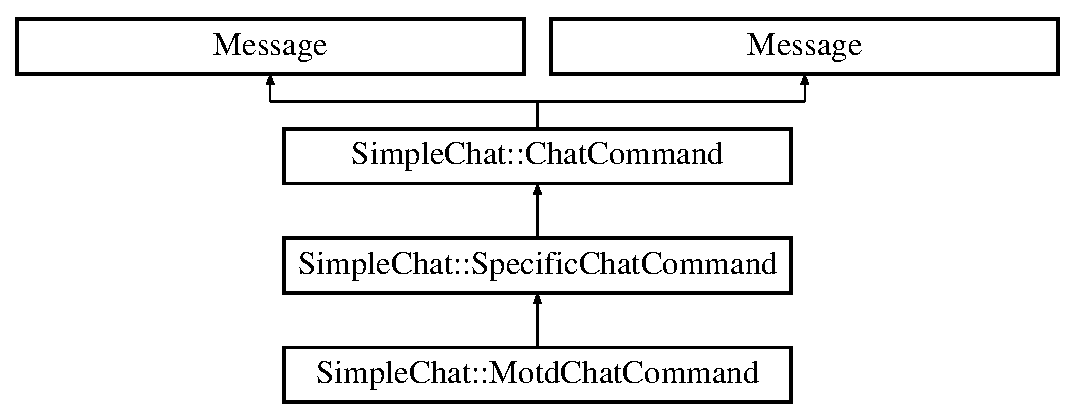
\includegraphics[height=4.000000cm]{classSimpleChat_1_1MotdChatCommand}
\end{center}
\end{figure}
\subsection*{Public Member Functions}
\begin{DoxyCompactItemize}
\item 
virtual void \hyperlink{classSimpleChat_1_1MotdChatCommand_a0fb363098dd591f712d894aac5e774b5}{insert\-Data} (const std\-::vector$<$ std\-::string $>$ \&arguments) override
\end{DoxyCompactItemize}
\subsection*{Additional Inherited Members}


\subsection{Member Function Documentation}
\hypertarget{classSimpleChat_1_1MotdChatCommand_a0fb363098dd591f712d894aac5e774b5}{\index{Simple\-Chat\-::\-Motd\-Chat\-Command@{Simple\-Chat\-::\-Motd\-Chat\-Command}!insert\-Data@{insert\-Data}}
\index{insert\-Data@{insert\-Data}!SimpleChat::MotdChatCommand@{Simple\-Chat\-::\-Motd\-Chat\-Command}}
\subsubsection[{insert\-Data}]{\setlength{\rightskip}{0pt plus 5cm}void Simple\-Chat\-::\-Motd\-Chat\-Command\-::insert\-Data (
\begin{DoxyParamCaption}
\item[{const std\-::vector$<$ std\-::string $>$ \&}]{arguments}
\end{DoxyParamCaption}
)\hspace{0.3cm}{\ttfamily [override]}, {\ttfamily [virtual]}}}\label{classSimpleChat_1_1MotdChatCommand_a0fb363098dd591f712d894aac5e774b5}
join all arguments because motd can contain spaces 

Implements \hyperlink{classSimpleChat_1_1SpecificChatCommand}{Simple\-Chat\-::\-Specific\-Chat\-Command}.



The documentation for this class was generated from the following files\-:\begin{DoxyCompactItemize}
\item 
chatlib/chat/commands/Motd\-Chat\-Command.\-h\item 
chatlib/chat/commands/Motd\-Chat\-Command.\-cpp\end{DoxyCompactItemize}

\hypertarget{classSimpleChat_1_1MuteChatCommand}{\section{Simple\-Chat\-:\-:Mute\-Chat\-Command Class Reference}
\label{classSimpleChat_1_1MuteChatCommand}\index{Simple\-Chat\-::\-Mute\-Chat\-Command@{Simple\-Chat\-::\-Mute\-Chat\-Command}}
}
Inheritance diagram for Simple\-Chat\-:\-:Mute\-Chat\-Command\-:\begin{figure}[H]
\begin{center}
\leavevmode
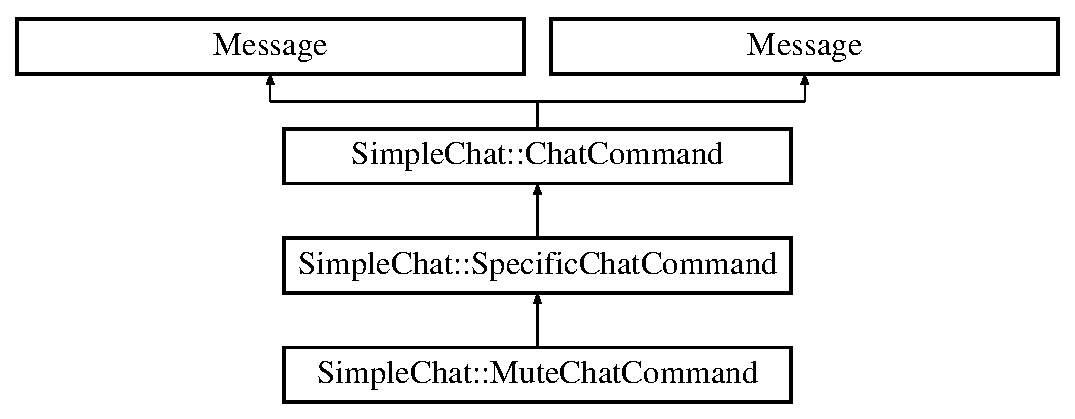
\includegraphics[height=4.000000cm]{classSimpleChat_1_1MuteChatCommand}
\end{center}
\end{figure}
\subsection*{Public Member Functions}
\begin{DoxyCompactItemize}
\item 
\hypertarget{classSimpleChat_1_1MuteChatCommand_ae140c788f937655702e0d5329ce29724}{virtual void {\bfseries insert\-Data} (const std\-::vector$<$ std\-::string $>$ \&arguments) override}\label{classSimpleChat_1_1MuteChatCommand_ae140c788f937655702e0d5329ce29724}

\end{DoxyCompactItemize}
\subsection*{Additional Inherited Members}


The documentation for this class was generated from the following files\-:\begin{DoxyCompactItemize}
\item 
chatlib/chat/commands/Mute\-Chat\-Command.\-h\item 
chatlib/chat/commands/Mute\-Chat\-Command.\-cpp\end{DoxyCompactItemize}

\hypertarget{classSimpleChat_1_1NetworkMessage}{\section{Simple\-Chat\-:\-:Network\-Message Class Reference}
\label{classSimpleChat_1_1NetworkMessage}\index{Simple\-Chat\-::\-Network\-Message@{Simple\-Chat\-::\-Network\-Message}}
}
Inheritance diagram for Simple\-Chat\-:\-:Network\-Message\-:\begin{figure}[H]
\begin{center}
\leavevmode
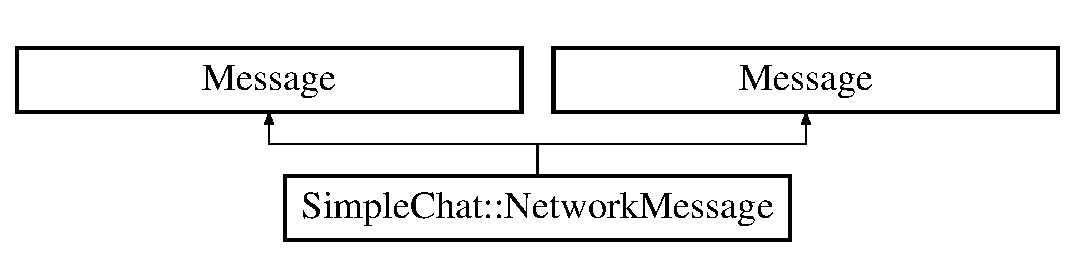
\includegraphics[height=2.000000cm]{classSimpleChat_1_1NetworkMessage}
\end{center}
\end{figure}
\subsection*{Public Member Functions}
\begin{DoxyCompactItemize}
\item 
\hypertarget{classSimpleChat_1_1NetworkMessage_adb9c3990b39bd7fa4d21fe1fe3710230}{{\bfseries Network\-Message} (const \hyperlink{classSimpleChat_1_1NetworkMessage}{Network\-Message} \&from)}\label{classSimpleChat_1_1NetworkMessage_adb9c3990b39bd7fa4d21fe1fe3710230}

\item 
\hypertarget{classSimpleChat_1_1NetworkMessage_a2ca0a232b03313c7150c3cdf295b2fd3}{\hyperlink{classSimpleChat_1_1NetworkMessage}{Network\-Message} \& {\bfseries operator=} (const \hyperlink{classSimpleChat_1_1NetworkMessage}{Network\-Message} \&from)}\label{classSimpleChat_1_1NetworkMessage_a2ca0a232b03313c7150c3cdf295b2fd3}

\item 
\hypertarget{classSimpleChat_1_1NetworkMessage_aff73981217a39c278a2f2eb74a938d77}{const \\*
\-::google\-::protobuf\-::\-Unknown\-Field\-Set \& {\bfseries unknown\-\_\-fields} () const }\label{classSimpleChat_1_1NetworkMessage_aff73981217a39c278a2f2eb74a938d77}

\item 
\hypertarget{classSimpleChat_1_1NetworkMessage_a7d2913fbffd9f3bbf4c4c6f8c0688996}{inline\-::google\-::protobuf\-::\-Unknown\-Field\-Set $\ast$ {\bfseries mutable\-\_\-unknown\-\_\-fields} ()}\label{classSimpleChat_1_1NetworkMessage_a7d2913fbffd9f3bbf4c4c6f8c0688996}

\item 
\hypertarget{classSimpleChat_1_1NetworkMessage_a2ee30e7f81715ebabb0da01058268964}{void {\bfseries Swap} (\hyperlink{classSimpleChat_1_1NetworkMessage}{Network\-Message} $\ast$other)}\label{classSimpleChat_1_1NetworkMessage_a2ee30e7f81715ebabb0da01058268964}

\item 
\hypertarget{classSimpleChat_1_1NetworkMessage_ad8480eec6be5086ffd63ccbfb0f2ae27}{\hyperlink{classSimpleChat_1_1NetworkMessage}{Network\-Message} $\ast$ {\bfseries New} () const }\label{classSimpleChat_1_1NetworkMessage_ad8480eec6be5086ffd63ccbfb0f2ae27}

\item 
\hypertarget{classSimpleChat_1_1NetworkMessage_a0a05f8f5dd8138da2f3de39de8043ff2}{\hyperlink{classSimpleChat_1_1NetworkMessage}{Network\-Message} $\ast$ {\bfseries New} (\-::google\-::protobuf\-::\-Arena $\ast$arena) const }\label{classSimpleChat_1_1NetworkMessage_a0a05f8f5dd8138da2f3de39de8043ff2}

\item 
\hypertarget{classSimpleChat_1_1NetworkMessage_a13212b0add820b37943801510adf68e6}{void {\bfseries Copy\-From} (const \-::google\-::protobuf\-::\-Message \&from)}\label{classSimpleChat_1_1NetworkMessage_a13212b0add820b37943801510adf68e6}

\item 
\hypertarget{classSimpleChat_1_1NetworkMessage_a4ebdf50d9a86c243fe00ba7b5f913a35}{void {\bfseries Merge\-From} (const \-::google\-::protobuf\-::\-Message \&from)}\label{classSimpleChat_1_1NetworkMessage_a4ebdf50d9a86c243fe00ba7b5f913a35}

\item 
\hypertarget{classSimpleChat_1_1NetworkMessage_a7fbc5949aaa3375591fc084407add520}{void {\bfseries Copy\-From} (const \hyperlink{classSimpleChat_1_1NetworkMessage}{Network\-Message} \&from)}\label{classSimpleChat_1_1NetworkMessage_a7fbc5949aaa3375591fc084407add520}

\item 
\hypertarget{classSimpleChat_1_1NetworkMessage_a6515a8b8adf203fd8bedb18db80b0e74}{void {\bfseries Merge\-From} (const \hyperlink{classSimpleChat_1_1NetworkMessage}{Network\-Message} \&from)}\label{classSimpleChat_1_1NetworkMessage_a6515a8b8adf203fd8bedb18db80b0e74}

\item 
\hypertarget{classSimpleChat_1_1NetworkMessage_afde8955d5b8daa35c399519b8a2c2f71}{void {\bfseries Clear} ()}\label{classSimpleChat_1_1NetworkMessage_afde8955d5b8daa35c399519b8a2c2f71}

\item 
\hypertarget{classSimpleChat_1_1NetworkMessage_afa900a259b82c3ea24e46ed98c5218c1}{bool {\bfseries Is\-Initialized} () const }\label{classSimpleChat_1_1NetworkMessage_afa900a259b82c3ea24e46ed98c5218c1}

\item 
\hypertarget{classSimpleChat_1_1NetworkMessage_a9245cbc44a5b79bab63bfc6abb599228}{int {\bfseries Byte\-Size} () const }\label{classSimpleChat_1_1NetworkMessage_a9245cbc44a5b79bab63bfc6abb599228}

\item 
\hypertarget{classSimpleChat_1_1NetworkMessage_a253f261555a96b562812625ed49678e1}{bool {\bfseries Merge\-Partial\-From\-Coded\-Stream} (\-::google\-::protobuf\-::io\-::\-Coded\-Input\-Stream $\ast$input)}\label{classSimpleChat_1_1NetworkMessage_a253f261555a96b562812625ed49678e1}

\item 
\hypertarget{classSimpleChat_1_1NetworkMessage_ab6b3953b6b07078c18ea42f7c81ba957}{void {\bfseries Serialize\-With\-Cached\-Sizes} (\-::google\-::protobuf\-::io\-::\-Coded\-Output\-Stream $\ast$output) const }\label{classSimpleChat_1_1NetworkMessage_ab6b3953b6b07078c18ea42f7c81ba957}

\item 
\hypertarget{classSimpleChat_1_1NetworkMessage_afbc3848b3ae57b9ac4fcb4a1066386a7}{\-::google\-::protobuf\-::uint8 $\ast$ {\bfseries Serialize\-With\-Cached\-Sizes\-To\-Array} (\-::google\-::protobuf\-::uint8 $\ast$output) const }\label{classSimpleChat_1_1NetworkMessage_afbc3848b3ae57b9ac4fcb4a1066386a7}

\item 
\hypertarget{classSimpleChat_1_1NetworkMessage_a9da9957343256049926de81427192a3e}{int {\bfseries Get\-Cached\-Size} () const }\label{classSimpleChat_1_1NetworkMessage_a9da9957343256049926de81427192a3e}

\item 
\hypertarget{classSimpleChat_1_1NetworkMessage_a353ea5839a3f4094ff329555be0deb80}{\-::google\-::protobuf\-::\-Metadata {\bfseries Get\-Metadata} () const }\label{classSimpleChat_1_1NetworkMessage_a353ea5839a3f4094ff329555be0deb80}

\item 
\hypertarget{classSimpleChat_1_1NetworkMessage_aa690cbc56fe136ebff5f2cd7cb2d1bf3}{bool {\bfseries has\-\_\-header} () const }\label{classSimpleChat_1_1NetworkMessage_aa690cbc56fe136ebff5f2cd7cb2d1bf3}

\item 
\hypertarget{classSimpleChat_1_1NetworkMessage_a4aa5e63844f15435b24365e56dcca8bf}{void {\bfseries clear\-\_\-header} ()}\label{classSimpleChat_1_1NetworkMessage_a4aa5e63844f15435b24365e56dcca8bf}

\item 
\hypertarget{classSimpleChat_1_1NetworkMessage_aa9e813c66ce0a4cde812988f9e32296a}{const \\*
\-::\hyperlink{classSimpleChat_1_1NetworkMessageHeader}{Simple\-Chat\-::\-Network\-Message\-Header} \& {\bfseries header} () const }\label{classSimpleChat_1_1NetworkMessage_aa9e813c66ce0a4cde812988f9e32296a}

\item 
\hypertarget{classSimpleChat_1_1NetworkMessage_a2b505ba16122a5466124623533110265}{\-::\hyperlink{classSimpleChat_1_1NetworkMessageHeader}{Simple\-Chat\-::\-Network\-Message\-Header} $\ast$ {\bfseries mutable\-\_\-header} ()}\label{classSimpleChat_1_1NetworkMessage_a2b505ba16122a5466124623533110265}

\item 
\hypertarget{classSimpleChat_1_1NetworkMessage_a9e88e4532462d9e38633c67cffb07534}{\-::\hyperlink{classSimpleChat_1_1NetworkMessageHeader}{Simple\-Chat\-::\-Network\-Message\-Header} $\ast$ {\bfseries release\-\_\-header} ()}\label{classSimpleChat_1_1NetworkMessage_a9e88e4532462d9e38633c67cffb07534}

\item 
\hypertarget{classSimpleChat_1_1NetworkMessage_aa51b7ba1decb1797dfd093650ba08dad}{void {\bfseries set\-\_\-allocated\-\_\-header} (\-::\hyperlink{classSimpleChat_1_1NetworkMessageHeader}{Simple\-Chat\-::\-Network\-Message\-Header} $\ast$header)}\label{classSimpleChat_1_1NetworkMessage_aa51b7ba1decb1797dfd093650ba08dad}

\item 
\hypertarget{classSimpleChat_1_1NetworkMessage_a49bb324a3189bc0a0bb625b213271525}{bool {\bfseries has\-\_\-serialized\-\_\-data} () const }\label{classSimpleChat_1_1NetworkMessage_a49bb324a3189bc0a0bb625b213271525}

\item 
\hypertarget{classSimpleChat_1_1NetworkMessage_a72d633cac4a0124182d324b69580e87f}{void {\bfseries clear\-\_\-serialized\-\_\-data} ()}\label{classSimpleChat_1_1NetworkMessage_a72d633cac4a0124182d324b69580e87f}

\item 
\hypertarget{classSimpleChat_1_1NetworkMessage_a689794b9b421d674c50d925a3efd2bba}{const \-::std\-::string \& {\bfseries serialized\-\_\-data} () const }\label{classSimpleChat_1_1NetworkMessage_a689794b9b421d674c50d925a3efd2bba}

\item 
\hypertarget{classSimpleChat_1_1NetworkMessage_aa019206f91b409b2df833901ae5b7550}{void {\bfseries set\-\_\-serialized\-\_\-data} (const \-::std\-::string \&value)}\label{classSimpleChat_1_1NetworkMessage_aa019206f91b409b2df833901ae5b7550}

\item 
\hypertarget{classSimpleChat_1_1NetworkMessage_aef9c1f1afdf935e6195c07c99c0f2bdf}{void {\bfseries set\-\_\-serialized\-\_\-data} (const char $\ast$value)}\label{classSimpleChat_1_1NetworkMessage_aef9c1f1afdf935e6195c07c99c0f2bdf}

\item 
\hypertarget{classSimpleChat_1_1NetworkMessage_a8747f5041d73f390f233f6d31d21b1ae}{void {\bfseries set\-\_\-serialized\-\_\-data} (const void $\ast$value, size\-\_\-t size)}\label{classSimpleChat_1_1NetworkMessage_a8747f5041d73f390f233f6d31d21b1ae}

\item 
\hypertarget{classSimpleChat_1_1NetworkMessage_a8f88634ab28deb0db90170be7d384c60}{\-::std\-::string $\ast$ {\bfseries mutable\-\_\-serialized\-\_\-data} ()}\label{classSimpleChat_1_1NetworkMessage_a8f88634ab28deb0db90170be7d384c60}

\item 
\hypertarget{classSimpleChat_1_1NetworkMessage_a9f1c91bc27b77861710ccec760e13408}{\-::std\-::string $\ast$ {\bfseries release\-\_\-serialized\-\_\-data} ()}\label{classSimpleChat_1_1NetworkMessage_a9f1c91bc27b77861710ccec760e13408}

\item 
\hypertarget{classSimpleChat_1_1NetworkMessage_ae47d82ed0348f240dfd418dcacd9f8da}{void {\bfseries set\-\_\-allocated\-\_\-serialized\-\_\-data} (\-::std\-::string $\ast$serialized\-\_\-data)}\label{classSimpleChat_1_1NetworkMessage_ae47d82ed0348f240dfd418dcacd9f8da}

\item 
\hypertarget{classSimpleChat_1_1NetworkMessage_adb9c3990b39bd7fa4d21fe1fe3710230}{{\bfseries Network\-Message} (const \hyperlink{classSimpleChat_1_1NetworkMessage}{Network\-Message} \&from)}\label{classSimpleChat_1_1NetworkMessage_adb9c3990b39bd7fa4d21fe1fe3710230}

\item 
\hypertarget{classSimpleChat_1_1NetworkMessage_a2ca0a232b03313c7150c3cdf295b2fd3}{\hyperlink{classSimpleChat_1_1NetworkMessage}{Network\-Message} \& {\bfseries operator=} (const \hyperlink{classSimpleChat_1_1NetworkMessage}{Network\-Message} \&from)}\label{classSimpleChat_1_1NetworkMessage_a2ca0a232b03313c7150c3cdf295b2fd3}

\item 
\hypertarget{classSimpleChat_1_1NetworkMessage_aff73981217a39c278a2f2eb74a938d77}{const \\*
\-::google\-::protobuf\-::\-Unknown\-Field\-Set \& {\bfseries unknown\-\_\-fields} () const }\label{classSimpleChat_1_1NetworkMessage_aff73981217a39c278a2f2eb74a938d77}

\item 
\hypertarget{classSimpleChat_1_1NetworkMessage_a7d2913fbffd9f3bbf4c4c6f8c0688996}{inline\-::google\-::protobuf\-::\-Unknown\-Field\-Set $\ast$ {\bfseries mutable\-\_\-unknown\-\_\-fields} ()}\label{classSimpleChat_1_1NetworkMessage_a7d2913fbffd9f3bbf4c4c6f8c0688996}

\item 
\hypertarget{classSimpleChat_1_1NetworkMessage_a2ee30e7f81715ebabb0da01058268964}{void {\bfseries Swap} (\hyperlink{classSimpleChat_1_1NetworkMessage}{Network\-Message} $\ast$other)}\label{classSimpleChat_1_1NetworkMessage_a2ee30e7f81715ebabb0da01058268964}

\item 
\hypertarget{classSimpleChat_1_1NetworkMessage_ad8480eec6be5086ffd63ccbfb0f2ae27}{\hyperlink{classSimpleChat_1_1NetworkMessage}{Network\-Message} $\ast$ {\bfseries New} () const }\label{classSimpleChat_1_1NetworkMessage_ad8480eec6be5086ffd63ccbfb0f2ae27}

\item 
\hypertarget{classSimpleChat_1_1NetworkMessage_a0a05f8f5dd8138da2f3de39de8043ff2}{\hyperlink{classSimpleChat_1_1NetworkMessage}{Network\-Message} $\ast$ {\bfseries New} (\-::google\-::protobuf\-::\-Arena $\ast$arena) const }\label{classSimpleChat_1_1NetworkMessage_a0a05f8f5dd8138da2f3de39de8043ff2}

\item 
\hypertarget{classSimpleChat_1_1NetworkMessage_a13212b0add820b37943801510adf68e6}{void {\bfseries Copy\-From} (const \-::google\-::protobuf\-::\-Message \&from)}\label{classSimpleChat_1_1NetworkMessage_a13212b0add820b37943801510adf68e6}

\item 
\hypertarget{classSimpleChat_1_1NetworkMessage_a4ebdf50d9a86c243fe00ba7b5f913a35}{void {\bfseries Merge\-From} (const \-::google\-::protobuf\-::\-Message \&from)}\label{classSimpleChat_1_1NetworkMessage_a4ebdf50d9a86c243fe00ba7b5f913a35}

\item 
\hypertarget{classSimpleChat_1_1NetworkMessage_a7fbc5949aaa3375591fc084407add520}{void {\bfseries Copy\-From} (const \hyperlink{classSimpleChat_1_1NetworkMessage}{Network\-Message} \&from)}\label{classSimpleChat_1_1NetworkMessage_a7fbc5949aaa3375591fc084407add520}

\item 
\hypertarget{classSimpleChat_1_1NetworkMessage_a6515a8b8adf203fd8bedb18db80b0e74}{void {\bfseries Merge\-From} (const \hyperlink{classSimpleChat_1_1NetworkMessage}{Network\-Message} \&from)}\label{classSimpleChat_1_1NetworkMessage_a6515a8b8adf203fd8bedb18db80b0e74}

\item 
\hypertarget{classSimpleChat_1_1NetworkMessage_afde8955d5b8daa35c399519b8a2c2f71}{void {\bfseries Clear} ()}\label{classSimpleChat_1_1NetworkMessage_afde8955d5b8daa35c399519b8a2c2f71}

\item 
\hypertarget{classSimpleChat_1_1NetworkMessage_afa900a259b82c3ea24e46ed98c5218c1}{bool {\bfseries Is\-Initialized} () const }\label{classSimpleChat_1_1NetworkMessage_afa900a259b82c3ea24e46ed98c5218c1}

\item 
\hypertarget{classSimpleChat_1_1NetworkMessage_a9245cbc44a5b79bab63bfc6abb599228}{int {\bfseries Byte\-Size} () const }\label{classSimpleChat_1_1NetworkMessage_a9245cbc44a5b79bab63bfc6abb599228}

\item 
\hypertarget{classSimpleChat_1_1NetworkMessage_a253f261555a96b562812625ed49678e1}{bool {\bfseries Merge\-Partial\-From\-Coded\-Stream} (\-::google\-::protobuf\-::io\-::\-Coded\-Input\-Stream $\ast$input)}\label{classSimpleChat_1_1NetworkMessage_a253f261555a96b562812625ed49678e1}

\item 
\hypertarget{classSimpleChat_1_1NetworkMessage_ab6b3953b6b07078c18ea42f7c81ba957}{void {\bfseries Serialize\-With\-Cached\-Sizes} (\-::google\-::protobuf\-::io\-::\-Coded\-Output\-Stream $\ast$output) const }\label{classSimpleChat_1_1NetworkMessage_ab6b3953b6b07078c18ea42f7c81ba957}

\item 
\hypertarget{classSimpleChat_1_1NetworkMessage_afbc3848b3ae57b9ac4fcb4a1066386a7}{\-::google\-::protobuf\-::uint8 $\ast$ {\bfseries Serialize\-With\-Cached\-Sizes\-To\-Array} (\-::google\-::protobuf\-::uint8 $\ast$output) const }\label{classSimpleChat_1_1NetworkMessage_afbc3848b3ae57b9ac4fcb4a1066386a7}

\item 
\hypertarget{classSimpleChat_1_1NetworkMessage_a9da9957343256049926de81427192a3e}{int {\bfseries Get\-Cached\-Size} () const }\label{classSimpleChat_1_1NetworkMessage_a9da9957343256049926de81427192a3e}

\item 
\hypertarget{classSimpleChat_1_1NetworkMessage_a353ea5839a3f4094ff329555be0deb80}{\-::google\-::protobuf\-::\-Metadata {\bfseries Get\-Metadata} () const }\label{classSimpleChat_1_1NetworkMessage_a353ea5839a3f4094ff329555be0deb80}

\item 
\hypertarget{classSimpleChat_1_1NetworkMessage_aa690cbc56fe136ebff5f2cd7cb2d1bf3}{bool {\bfseries has\-\_\-header} () const }\label{classSimpleChat_1_1NetworkMessage_aa690cbc56fe136ebff5f2cd7cb2d1bf3}

\item 
\hypertarget{classSimpleChat_1_1NetworkMessage_a4aa5e63844f15435b24365e56dcca8bf}{void {\bfseries clear\-\_\-header} ()}\label{classSimpleChat_1_1NetworkMessage_a4aa5e63844f15435b24365e56dcca8bf}

\item 
\hypertarget{classSimpleChat_1_1NetworkMessage_a806f88019d6567da8428b3e32ddc9b80}{const \\*
\-::\hyperlink{classSimpleChat_1_1NetworkMessageHeader}{Simple\-Chat\-::\-Network\-Message\-Header} \& {\bfseries header} () const }\label{classSimpleChat_1_1NetworkMessage_a806f88019d6567da8428b3e32ddc9b80}

\item 
\hypertarget{classSimpleChat_1_1NetworkMessage_af5b511d2ddfa706a411919d5f828c19a}{\-::\hyperlink{classSimpleChat_1_1NetworkMessageHeader}{Simple\-Chat\-::\-Network\-Message\-Header} $\ast$ {\bfseries mutable\-\_\-header} ()}\label{classSimpleChat_1_1NetworkMessage_af5b511d2ddfa706a411919d5f828c19a}

\item 
\hypertarget{classSimpleChat_1_1NetworkMessage_ac75bcde248ca76cc4aa7f839247c304a}{\-::\hyperlink{classSimpleChat_1_1NetworkMessageHeader}{Simple\-Chat\-::\-Network\-Message\-Header} $\ast$ {\bfseries release\-\_\-header} ()}\label{classSimpleChat_1_1NetworkMessage_ac75bcde248ca76cc4aa7f839247c304a}

\item 
\hypertarget{classSimpleChat_1_1NetworkMessage_aa51b7ba1decb1797dfd093650ba08dad}{void {\bfseries set\-\_\-allocated\-\_\-header} (\-::\hyperlink{classSimpleChat_1_1NetworkMessageHeader}{Simple\-Chat\-::\-Network\-Message\-Header} $\ast$header)}\label{classSimpleChat_1_1NetworkMessage_aa51b7ba1decb1797dfd093650ba08dad}

\item 
\hypertarget{classSimpleChat_1_1NetworkMessage_a49bb324a3189bc0a0bb625b213271525}{bool {\bfseries has\-\_\-serialized\-\_\-data} () const }\label{classSimpleChat_1_1NetworkMessage_a49bb324a3189bc0a0bb625b213271525}

\item 
\hypertarget{classSimpleChat_1_1NetworkMessage_a72d633cac4a0124182d324b69580e87f}{void {\bfseries clear\-\_\-serialized\-\_\-data} ()}\label{classSimpleChat_1_1NetworkMessage_a72d633cac4a0124182d324b69580e87f}

\item 
\hypertarget{classSimpleChat_1_1NetworkMessage_a4e73beaedd4eaa119c980d4a9cb346d3}{const \-::std\-::string \& {\bfseries serialized\-\_\-data} () const }\label{classSimpleChat_1_1NetworkMessage_a4e73beaedd4eaa119c980d4a9cb346d3}

\item 
\hypertarget{classSimpleChat_1_1NetworkMessage_aa019206f91b409b2df833901ae5b7550}{void {\bfseries set\-\_\-serialized\-\_\-data} (const \-::std\-::string \&value)}\label{classSimpleChat_1_1NetworkMessage_aa019206f91b409b2df833901ae5b7550}

\item 
\hypertarget{classSimpleChat_1_1NetworkMessage_aef9c1f1afdf935e6195c07c99c0f2bdf}{void {\bfseries set\-\_\-serialized\-\_\-data} (const char $\ast$value)}\label{classSimpleChat_1_1NetworkMessage_aef9c1f1afdf935e6195c07c99c0f2bdf}

\item 
\hypertarget{classSimpleChat_1_1NetworkMessage_a8747f5041d73f390f233f6d31d21b1ae}{void {\bfseries set\-\_\-serialized\-\_\-data} (const void $\ast$value, size\-\_\-t size)}\label{classSimpleChat_1_1NetworkMessage_a8747f5041d73f390f233f6d31d21b1ae}

\item 
\hypertarget{classSimpleChat_1_1NetworkMessage_a545fbed2c2b950761a9121432ee36071}{\-::std\-::string $\ast$ {\bfseries mutable\-\_\-serialized\-\_\-data} ()}\label{classSimpleChat_1_1NetworkMessage_a545fbed2c2b950761a9121432ee36071}

\item 
\hypertarget{classSimpleChat_1_1NetworkMessage_a381746122f4698cb44e937539d9c6ddf}{\-::std\-::string $\ast$ {\bfseries release\-\_\-serialized\-\_\-data} ()}\label{classSimpleChat_1_1NetworkMessage_a381746122f4698cb44e937539d9c6ddf}

\item 
\hypertarget{classSimpleChat_1_1NetworkMessage_ae47d82ed0348f240dfd418dcacd9f8da}{void {\bfseries set\-\_\-allocated\-\_\-serialized\-\_\-data} (\-::std\-::string $\ast$serialized\-\_\-data)}\label{classSimpleChat_1_1NetworkMessage_ae47d82ed0348f240dfd418dcacd9f8da}

\end{DoxyCompactItemize}
\subsection*{Static Public Member Functions}
\begin{DoxyCompactItemize}
\item 
\hypertarget{classSimpleChat_1_1NetworkMessage_a950c1e8d9d7f50956eabcd02a399c5b9}{static const \\*
\-::google\-::protobuf\-::\-Descriptor $\ast$ {\bfseries descriptor} ()}\label{classSimpleChat_1_1NetworkMessage_a950c1e8d9d7f50956eabcd02a399c5b9}

\item 
\hypertarget{classSimpleChat_1_1NetworkMessage_abbcdc7abd1b4c2ebdf8ce1ab683d3d03}{static const \hyperlink{classSimpleChat_1_1NetworkMessage}{Network\-Message} \& {\bfseries default\-\_\-instance} ()}\label{classSimpleChat_1_1NetworkMessage_abbcdc7abd1b4c2ebdf8ce1ab683d3d03}

\item 
\hypertarget{classSimpleChat_1_1NetworkMessage_a950c1e8d9d7f50956eabcd02a399c5b9}{static const \\*
\-::google\-::protobuf\-::\-Descriptor $\ast$ {\bfseries descriptor} ()}\label{classSimpleChat_1_1NetworkMessage_a950c1e8d9d7f50956eabcd02a399c5b9}

\item 
\hypertarget{classSimpleChat_1_1NetworkMessage_abbcdc7abd1b4c2ebdf8ce1ab683d3d03}{static const \hyperlink{classSimpleChat_1_1NetworkMessage}{Network\-Message} \& {\bfseries default\-\_\-instance} ()}\label{classSimpleChat_1_1NetworkMessage_abbcdc7abd1b4c2ebdf8ce1ab683d3d03}

\end{DoxyCompactItemize}
\subsection*{Static Public Attributes}
\begin{DoxyCompactItemize}
\item 
\hypertarget{classSimpleChat_1_1NetworkMessage_a24821b9d09b0dc666322a5615092a7d6}{static const int {\bfseries k\-Header\-Field\-Number} = 1}\label{classSimpleChat_1_1NetworkMessage_a24821b9d09b0dc666322a5615092a7d6}

\item 
\hypertarget{classSimpleChat_1_1NetworkMessage_ac3bc296196533f7417d7be0b6977d2d4}{static const int {\bfseries k\-Serialized\-Data\-Field\-Number} = 2}\label{classSimpleChat_1_1NetworkMessage_ac3bc296196533f7417d7be0b6977d2d4}

\end{DoxyCompactItemize}
\subsection*{Friends}
\begin{DoxyCompactItemize}
\item 
\hypertarget{classSimpleChat_1_1NetworkMessage_a3486afd4adb1bba7588d52e4aabbca06}{void {\bfseries protobuf\-\_\-\-Add\-Desc\-\_\-\-Network\-Message\-\_\-2eproto} ()}\label{classSimpleChat_1_1NetworkMessage_a3486afd4adb1bba7588d52e4aabbca06}

\item 
\hypertarget{classSimpleChat_1_1NetworkMessage_af845200205064a98818e47c69988e43b}{void {\bfseries protobuf\-\_\-\-Assign\-Desc\-\_\-\-Network\-Message\-\_\-2eproto} ()}\label{classSimpleChat_1_1NetworkMessage_af845200205064a98818e47c69988e43b}

\item 
\hypertarget{classSimpleChat_1_1NetworkMessage_a5dd630836c26acd95825919f5d81def4}{void {\bfseries protobuf\-\_\-\-Shutdown\-File\-\_\-\-Network\-Message\-\_\-2eproto} ()}\label{classSimpleChat_1_1NetworkMessage_a5dd630836c26acd95825919f5d81def4}

\item 
\hypertarget{classSimpleChat_1_1NetworkMessage_a3486afd4adb1bba7588d52e4aabbca06}{void {\bfseries protobuf\-\_\-\-Add\-Desc\-\_\-\-Network\-Message\-\_\-2eproto} ()}\label{classSimpleChat_1_1NetworkMessage_a3486afd4adb1bba7588d52e4aabbca06}

\item 
\hypertarget{classSimpleChat_1_1NetworkMessage_af845200205064a98818e47c69988e43b}{void {\bfseries protobuf\-\_\-\-Assign\-Desc\-\_\-\-Network\-Message\-\_\-2eproto} ()}\label{classSimpleChat_1_1NetworkMessage_af845200205064a98818e47c69988e43b}

\item 
\hypertarget{classSimpleChat_1_1NetworkMessage_a5dd630836c26acd95825919f5d81def4}{void {\bfseries protobuf\-\_\-\-Shutdown\-File\-\_\-\-Network\-Message\-\_\-2eproto} ()}\label{classSimpleChat_1_1NetworkMessage_a5dd630836c26acd95825919f5d81def4}

\end{DoxyCompactItemize}


The documentation for this class was generated from the following file\-:\begin{DoxyCompactItemize}
\item 
chatlib/proto/Network\-Message.\-pb.\-h\end{DoxyCompactItemize}

\hypertarget{classSimpleChat_1_1NetworkMessageHeader}{\section{Simple\-Chat\-:\-:Network\-Message\-Header Class Reference}
\label{classSimpleChat_1_1NetworkMessageHeader}\index{Simple\-Chat\-::\-Network\-Message\-Header@{Simple\-Chat\-::\-Network\-Message\-Header}}
}
Inheritance diagram for Simple\-Chat\-:\-:Network\-Message\-Header\-:\begin{figure}[H]
\begin{center}
\leavevmode
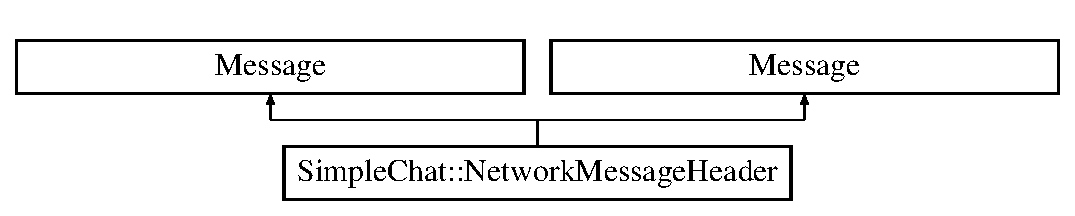
\includegraphics[height=2.000000cm]{classSimpleChat_1_1NetworkMessageHeader}
\end{center}
\end{figure}
\subsection*{Public Member Functions}
\begin{DoxyCompactItemize}
\item 
\hypertarget{classSimpleChat_1_1NetworkMessageHeader_a1d1af8dfcf0c03757ac9caf3d164b0e8}{{\bfseries Network\-Message\-Header} (const \hyperlink{classSimpleChat_1_1NetworkMessageHeader}{Network\-Message\-Header} \&from)}\label{classSimpleChat_1_1NetworkMessageHeader_a1d1af8dfcf0c03757ac9caf3d164b0e8}

\item 
\hypertarget{classSimpleChat_1_1NetworkMessageHeader_a2e9fe30dac33dfac80ac154ddcd0914a}{\hyperlink{classSimpleChat_1_1NetworkMessageHeader}{Network\-Message\-Header} \& {\bfseries operator=} (const \hyperlink{classSimpleChat_1_1NetworkMessageHeader}{Network\-Message\-Header} \&from)}\label{classSimpleChat_1_1NetworkMessageHeader_a2e9fe30dac33dfac80ac154ddcd0914a}

\item 
\hypertarget{classSimpleChat_1_1NetworkMessageHeader_a0d7814ba533eae44c26f024d84103e94}{const \\*
\-::google\-::protobuf\-::\-Unknown\-Field\-Set \& {\bfseries unknown\-\_\-fields} () const }\label{classSimpleChat_1_1NetworkMessageHeader_a0d7814ba533eae44c26f024d84103e94}

\item 
\hypertarget{classSimpleChat_1_1NetworkMessageHeader_a3e1df7d2aa1262ef8e17e2f5fdad7d40}{inline\-::google\-::protobuf\-::\-Unknown\-Field\-Set $\ast$ {\bfseries mutable\-\_\-unknown\-\_\-fields} ()}\label{classSimpleChat_1_1NetworkMessageHeader_a3e1df7d2aa1262ef8e17e2f5fdad7d40}

\item 
\hypertarget{classSimpleChat_1_1NetworkMessageHeader_ac12a19d7792504929483161b3489106d}{void {\bfseries Swap} (\hyperlink{classSimpleChat_1_1NetworkMessageHeader}{Network\-Message\-Header} $\ast$other)}\label{classSimpleChat_1_1NetworkMessageHeader_ac12a19d7792504929483161b3489106d}

\item 
\hypertarget{classSimpleChat_1_1NetworkMessageHeader_a6ceb4050a7cd60080404951418794879}{\hyperlink{classSimpleChat_1_1NetworkMessageHeader}{Network\-Message\-Header} $\ast$ {\bfseries New} () const }\label{classSimpleChat_1_1NetworkMessageHeader_a6ceb4050a7cd60080404951418794879}

\item 
\hypertarget{classSimpleChat_1_1NetworkMessageHeader_aeb297b2d6557953e416b452460587c2d}{\hyperlink{classSimpleChat_1_1NetworkMessageHeader}{Network\-Message\-Header} $\ast$ {\bfseries New} (\-::google\-::protobuf\-::\-Arena $\ast$arena) const }\label{classSimpleChat_1_1NetworkMessageHeader_aeb297b2d6557953e416b452460587c2d}

\item 
\hypertarget{classSimpleChat_1_1NetworkMessageHeader_ac53c26c6d84a5116fb42d70a53008303}{void {\bfseries Copy\-From} (const \-::google\-::protobuf\-::\-Message \&from)}\label{classSimpleChat_1_1NetworkMessageHeader_ac53c26c6d84a5116fb42d70a53008303}

\item 
\hypertarget{classSimpleChat_1_1NetworkMessageHeader_a6205622710d8485ab9ffd8d794631cfc}{void {\bfseries Merge\-From} (const \-::google\-::protobuf\-::\-Message \&from)}\label{classSimpleChat_1_1NetworkMessageHeader_a6205622710d8485ab9ffd8d794631cfc}

\item 
\hypertarget{classSimpleChat_1_1NetworkMessageHeader_ab460c8fa9abd6314b0cf49be2c6e26de}{void {\bfseries Copy\-From} (const \hyperlink{classSimpleChat_1_1NetworkMessageHeader}{Network\-Message\-Header} \&from)}\label{classSimpleChat_1_1NetworkMessageHeader_ab460c8fa9abd6314b0cf49be2c6e26de}

\item 
\hypertarget{classSimpleChat_1_1NetworkMessageHeader_a02696f7c2f6bbff7c82f64fd1f615599}{void {\bfseries Merge\-From} (const \hyperlink{classSimpleChat_1_1NetworkMessageHeader}{Network\-Message\-Header} \&from)}\label{classSimpleChat_1_1NetworkMessageHeader_a02696f7c2f6bbff7c82f64fd1f615599}

\item 
\hypertarget{classSimpleChat_1_1NetworkMessageHeader_a33544fbb349ce8275b334e31d4e708f4}{void {\bfseries Clear} ()}\label{classSimpleChat_1_1NetworkMessageHeader_a33544fbb349ce8275b334e31d4e708f4}

\item 
\hypertarget{classSimpleChat_1_1NetworkMessageHeader_acc0a30d58655083c79af4472f7aee3a2}{bool {\bfseries Is\-Initialized} () const }\label{classSimpleChat_1_1NetworkMessageHeader_acc0a30d58655083c79af4472f7aee3a2}

\item 
\hypertarget{classSimpleChat_1_1NetworkMessageHeader_a3e2312da986374bf537e1c173eb220a1}{int {\bfseries Byte\-Size} () const }\label{classSimpleChat_1_1NetworkMessageHeader_a3e2312da986374bf537e1c173eb220a1}

\item 
\hypertarget{classSimpleChat_1_1NetworkMessageHeader_a2581c3d79e42bd4d3ac450a4437852c4}{bool {\bfseries Merge\-Partial\-From\-Coded\-Stream} (\-::google\-::protobuf\-::io\-::\-Coded\-Input\-Stream $\ast$input)}\label{classSimpleChat_1_1NetworkMessageHeader_a2581c3d79e42bd4d3ac450a4437852c4}

\item 
\hypertarget{classSimpleChat_1_1NetworkMessageHeader_a01d04719c32328fb2bb106e89790fd72}{void {\bfseries Serialize\-With\-Cached\-Sizes} (\-::google\-::protobuf\-::io\-::\-Coded\-Output\-Stream $\ast$output) const }\label{classSimpleChat_1_1NetworkMessageHeader_a01d04719c32328fb2bb106e89790fd72}

\item 
\hypertarget{classSimpleChat_1_1NetworkMessageHeader_a23591751df56360a33c07b61206bde95}{\-::google\-::protobuf\-::uint8 $\ast$ {\bfseries Serialize\-With\-Cached\-Sizes\-To\-Array} (\-::google\-::protobuf\-::uint8 $\ast$output) const }\label{classSimpleChat_1_1NetworkMessageHeader_a23591751df56360a33c07b61206bde95}

\item 
\hypertarget{classSimpleChat_1_1NetworkMessageHeader_aa031119fe9b93440b129d9dea6f42c3d}{int {\bfseries Get\-Cached\-Size} () const }\label{classSimpleChat_1_1NetworkMessageHeader_aa031119fe9b93440b129d9dea6f42c3d}

\item 
\hypertarget{classSimpleChat_1_1NetworkMessageHeader_ad784a116c57d281e27fb07daaf1bb37e}{\-::google\-::protobuf\-::\-Metadata {\bfseries Get\-Metadata} () const }\label{classSimpleChat_1_1NetworkMessageHeader_ad784a116c57d281e27fb07daaf1bb37e}

\item 
\hypertarget{classSimpleChat_1_1NetworkMessageHeader_a053ce1d5b479c63b4eec557e5a329ff0}{bool {\bfseries has\-\_\-type} () const }\label{classSimpleChat_1_1NetworkMessageHeader_a053ce1d5b479c63b4eec557e5a329ff0}

\item 
\hypertarget{classSimpleChat_1_1NetworkMessageHeader_a370f33ee9694bedca599961ce3842678}{void {\bfseries clear\-\_\-type} ()}\label{classSimpleChat_1_1NetworkMessageHeader_a370f33ee9694bedca599961ce3842678}

\item 
\hypertarget{classSimpleChat_1_1NetworkMessageHeader_ae0edc205c59584f4ad6bcbc077ea23cb}{\-::Simple\-Chat\-::\-Network\-Message\-Type {\bfseries type} () const }\label{classSimpleChat_1_1NetworkMessageHeader_ae0edc205c59584f4ad6bcbc077ea23cb}

\item 
\hypertarget{classSimpleChat_1_1NetworkMessageHeader_a05389e5df449611dc1396b530cdb5f94}{void {\bfseries set\-\_\-type} (\-::Simple\-Chat\-::\-Network\-Message\-Type value)}\label{classSimpleChat_1_1NetworkMessageHeader_a05389e5df449611dc1396b530cdb5f94}

\item 
\hypertarget{classSimpleChat_1_1NetworkMessageHeader_a2464b223558059d6c278dc52286fc77a}{bool {\bfseries has\-\_\-size} () const }\label{classSimpleChat_1_1NetworkMessageHeader_a2464b223558059d6c278dc52286fc77a}

\item 
\hypertarget{classSimpleChat_1_1NetworkMessageHeader_a5fa0c823592084a7d356d5a473395109}{void {\bfseries clear\-\_\-size} ()}\label{classSimpleChat_1_1NetworkMessageHeader_a5fa0c823592084a7d356d5a473395109}

\item 
\hypertarget{classSimpleChat_1_1NetworkMessageHeader_a4d2c42bd336f021b6d87a3239fd9cabd}{\-::google\-::protobuf\-::int32 {\bfseries size} () const }\label{classSimpleChat_1_1NetworkMessageHeader_a4d2c42bd336f021b6d87a3239fd9cabd}

\item 
\hypertarget{classSimpleChat_1_1NetworkMessageHeader_a8a0c7559de32b473e6a92160973f406c}{void {\bfseries set\-\_\-size} (\-::google\-::protobuf\-::int32 value)}\label{classSimpleChat_1_1NetworkMessageHeader_a8a0c7559de32b473e6a92160973f406c}

\item 
\hypertarget{classSimpleChat_1_1NetworkMessageHeader_a1d1af8dfcf0c03757ac9caf3d164b0e8}{{\bfseries Network\-Message\-Header} (const \hyperlink{classSimpleChat_1_1NetworkMessageHeader}{Network\-Message\-Header} \&from)}\label{classSimpleChat_1_1NetworkMessageHeader_a1d1af8dfcf0c03757ac9caf3d164b0e8}

\item 
\hypertarget{classSimpleChat_1_1NetworkMessageHeader_a2e9fe30dac33dfac80ac154ddcd0914a}{\hyperlink{classSimpleChat_1_1NetworkMessageHeader}{Network\-Message\-Header} \& {\bfseries operator=} (const \hyperlink{classSimpleChat_1_1NetworkMessageHeader}{Network\-Message\-Header} \&from)}\label{classSimpleChat_1_1NetworkMessageHeader_a2e9fe30dac33dfac80ac154ddcd0914a}

\item 
\hypertarget{classSimpleChat_1_1NetworkMessageHeader_a0d7814ba533eae44c26f024d84103e94}{const \\*
\-::google\-::protobuf\-::\-Unknown\-Field\-Set \& {\bfseries unknown\-\_\-fields} () const }\label{classSimpleChat_1_1NetworkMessageHeader_a0d7814ba533eae44c26f024d84103e94}

\item 
\hypertarget{classSimpleChat_1_1NetworkMessageHeader_a3e1df7d2aa1262ef8e17e2f5fdad7d40}{inline\-::google\-::protobuf\-::\-Unknown\-Field\-Set $\ast$ {\bfseries mutable\-\_\-unknown\-\_\-fields} ()}\label{classSimpleChat_1_1NetworkMessageHeader_a3e1df7d2aa1262ef8e17e2f5fdad7d40}

\item 
\hypertarget{classSimpleChat_1_1NetworkMessageHeader_ac12a19d7792504929483161b3489106d}{void {\bfseries Swap} (\hyperlink{classSimpleChat_1_1NetworkMessageHeader}{Network\-Message\-Header} $\ast$other)}\label{classSimpleChat_1_1NetworkMessageHeader_ac12a19d7792504929483161b3489106d}

\item 
\hypertarget{classSimpleChat_1_1NetworkMessageHeader_a6ceb4050a7cd60080404951418794879}{\hyperlink{classSimpleChat_1_1NetworkMessageHeader}{Network\-Message\-Header} $\ast$ {\bfseries New} () const }\label{classSimpleChat_1_1NetworkMessageHeader_a6ceb4050a7cd60080404951418794879}

\item 
\hypertarget{classSimpleChat_1_1NetworkMessageHeader_aeb297b2d6557953e416b452460587c2d}{\hyperlink{classSimpleChat_1_1NetworkMessageHeader}{Network\-Message\-Header} $\ast$ {\bfseries New} (\-::google\-::protobuf\-::\-Arena $\ast$arena) const }\label{classSimpleChat_1_1NetworkMessageHeader_aeb297b2d6557953e416b452460587c2d}

\item 
\hypertarget{classSimpleChat_1_1NetworkMessageHeader_ac53c26c6d84a5116fb42d70a53008303}{void {\bfseries Copy\-From} (const \-::google\-::protobuf\-::\-Message \&from)}\label{classSimpleChat_1_1NetworkMessageHeader_ac53c26c6d84a5116fb42d70a53008303}

\item 
\hypertarget{classSimpleChat_1_1NetworkMessageHeader_a6205622710d8485ab9ffd8d794631cfc}{void {\bfseries Merge\-From} (const \-::google\-::protobuf\-::\-Message \&from)}\label{classSimpleChat_1_1NetworkMessageHeader_a6205622710d8485ab9ffd8d794631cfc}

\item 
\hypertarget{classSimpleChat_1_1NetworkMessageHeader_ab460c8fa9abd6314b0cf49be2c6e26de}{void {\bfseries Copy\-From} (const \hyperlink{classSimpleChat_1_1NetworkMessageHeader}{Network\-Message\-Header} \&from)}\label{classSimpleChat_1_1NetworkMessageHeader_ab460c8fa9abd6314b0cf49be2c6e26de}

\item 
\hypertarget{classSimpleChat_1_1NetworkMessageHeader_a02696f7c2f6bbff7c82f64fd1f615599}{void {\bfseries Merge\-From} (const \hyperlink{classSimpleChat_1_1NetworkMessageHeader}{Network\-Message\-Header} \&from)}\label{classSimpleChat_1_1NetworkMessageHeader_a02696f7c2f6bbff7c82f64fd1f615599}

\item 
\hypertarget{classSimpleChat_1_1NetworkMessageHeader_a33544fbb349ce8275b334e31d4e708f4}{void {\bfseries Clear} ()}\label{classSimpleChat_1_1NetworkMessageHeader_a33544fbb349ce8275b334e31d4e708f4}

\item 
\hypertarget{classSimpleChat_1_1NetworkMessageHeader_acc0a30d58655083c79af4472f7aee3a2}{bool {\bfseries Is\-Initialized} () const }\label{classSimpleChat_1_1NetworkMessageHeader_acc0a30d58655083c79af4472f7aee3a2}

\item 
\hypertarget{classSimpleChat_1_1NetworkMessageHeader_a3e2312da986374bf537e1c173eb220a1}{int {\bfseries Byte\-Size} () const }\label{classSimpleChat_1_1NetworkMessageHeader_a3e2312da986374bf537e1c173eb220a1}

\item 
\hypertarget{classSimpleChat_1_1NetworkMessageHeader_a2581c3d79e42bd4d3ac450a4437852c4}{bool {\bfseries Merge\-Partial\-From\-Coded\-Stream} (\-::google\-::protobuf\-::io\-::\-Coded\-Input\-Stream $\ast$input)}\label{classSimpleChat_1_1NetworkMessageHeader_a2581c3d79e42bd4d3ac450a4437852c4}

\item 
\hypertarget{classSimpleChat_1_1NetworkMessageHeader_a01d04719c32328fb2bb106e89790fd72}{void {\bfseries Serialize\-With\-Cached\-Sizes} (\-::google\-::protobuf\-::io\-::\-Coded\-Output\-Stream $\ast$output) const }\label{classSimpleChat_1_1NetworkMessageHeader_a01d04719c32328fb2bb106e89790fd72}

\item 
\hypertarget{classSimpleChat_1_1NetworkMessageHeader_a23591751df56360a33c07b61206bde95}{\-::google\-::protobuf\-::uint8 $\ast$ {\bfseries Serialize\-With\-Cached\-Sizes\-To\-Array} (\-::google\-::protobuf\-::uint8 $\ast$output) const }\label{classSimpleChat_1_1NetworkMessageHeader_a23591751df56360a33c07b61206bde95}

\item 
\hypertarget{classSimpleChat_1_1NetworkMessageHeader_aa031119fe9b93440b129d9dea6f42c3d}{int {\bfseries Get\-Cached\-Size} () const }\label{classSimpleChat_1_1NetworkMessageHeader_aa031119fe9b93440b129d9dea6f42c3d}

\item 
\hypertarget{classSimpleChat_1_1NetworkMessageHeader_ad784a116c57d281e27fb07daaf1bb37e}{\-::google\-::protobuf\-::\-Metadata {\bfseries Get\-Metadata} () const }\label{classSimpleChat_1_1NetworkMessageHeader_ad784a116c57d281e27fb07daaf1bb37e}

\item 
\hypertarget{classSimpleChat_1_1NetworkMessageHeader_a3208b076331cd05dca86a6d864475a33}{bool {\bfseries has\-\_\-src} () const }\label{classSimpleChat_1_1NetworkMessageHeader_a3208b076331cd05dca86a6d864475a33}

\item 
\hypertarget{classSimpleChat_1_1NetworkMessageHeader_ad19f0afefd51ce38be98c8ed4df85122}{void {\bfseries clear\-\_\-src} ()}\label{classSimpleChat_1_1NetworkMessageHeader_ad19f0afefd51ce38be98c8ed4df85122}

\item 
\hypertarget{classSimpleChat_1_1NetworkMessageHeader_ae5c31bd1c6f183b1227dbce3d4e6eccb}{const \-::std\-::string \& {\bfseries src} () const }\label{classSimpleChat_1_1NetworkMessageHeader_ae5c31bd1c6f183b1227dbce3d4e6eccb}

\item 
\hypertarget{classSimpleChat_1_1NetworkMessageHeader_a8a250d8c47831c475447b0103a848250}{void {\bfseries set\-\_\-src} (const \-::std\-::string \&value)}\label{classSimpleChat_1_1NetworkMessageHeader_a8a250d8c47831c475447b0103a848250}

\item 
\hypertarget{classSimpleChat_1_1NetworkMessageHeader_a379d99e5dd3b24e9bb7abb99eed96752}{void {\bfseries set\-\_\-src} (const char $\ast$value)}\label{classSimpleChat_1_1NetworkMessageHeader_a379d99e5dd3b24e9bb7abb99eed96752}

\item 
\hypertarget{classSimpleChat_1_1NetworkMessageHeader_aa2f2eee5756eb02e36d8d22551c426c2}{void {\bfseries set\-\_\-src} (const char $\ast$value, size\-\_\-t size)}\label{classSimpleChat_1_1NetworkMessageHeader_aa2f2eee5756eb02e36d8d22551c426c2}

\item 
\hypertarget{classSimpleChat_1_1NetworkMessageHeader_ae2f429f5be1554fc2d735331809d6b2f}{\-::std\-::string $\ast$ {\bfseries mutable\-\_\-src} ()}\label{classSimpleChat_1_1NetworkMessageHeader_ae2f429f5be1554fc2d735331809d6b2f}

\item 
\hypertarget{classSimpleChat_1_1NetworkMessageHeader_a079c015e3af8c158520d80026c5be886}{\-::std\-::string $\ast$ {\bfseries release\-\_\-src} ()}\label{classSimpleChat_1_1NetworkMessageHeader_a079c015e3af8c158520d80026c5be886}

\item 
\hypertarget{classSimpleChat_1_1NetworkMessageHeader_a24df02cdca248d48b8ea7ac9f98b3d7b}{void {\bfseries set\-\_\-allocated\-\_\-src} (\-::std\-::string $\ast$src)}\label{classSimpleChat_1_1NetworkMessageHeader_a24df02cdca248d48b8ea7ac9f98b3d7b}

\item 
\hypertarget{classSimpleChat_1_1NetworkMessageHeader_aec77074aea2abc1625fcd8ce0351ea32}{bool {\bfseries has\-\_\-dest} () const }\label{classSimpleChat_1_1NetworkMessageHeader_aec77074aea2abc1625fcd8ce0351ea32}

\item 
\hypertarget{classSimpleChat_1_1NetworkMessageHeader_a1913f106d1b262d066f77c12c9b09176}{void {\bfseries clear\-\_\-dest} ()}\label{classSimpleChat_1_1NetworkMessageHeader_a1913f106d1b262d066f77c12c9b09176}

\item 
\hypertarget{classSimpleChat_1_1NetworkMessageHeader_acfac6ed452244b172fa78ac8ed78246e}{const \-::std\-::string \& {\bfseries dest} () const }\label{classSimpleChat_1_1NetworkMessageHeader_acfac6ed452244b172fa78ac8ed78246e}

\item 
\hypertarget{classSimpleChat_1_1NetworkMessageHeader_a834a905e43cfaf64f84f22eb55675e87}{void {\bfseries set\-\_\-dest} (const \-::std\-::string \&value)}\label{classSimpleChat_1_1NetworkMessageHeader_a834a905e43cfaf64f84f22eb55675e87}

\item 
\hypertarget{classSimpleChat_1_1NetworkMessageHeader_ad157827d1f5fed9e4acd7baa2b112471}{void {\bfseries set\-\_\-dest} (const char $\ast$value)}\label{classSimpleChat_1_1NetworkMessageHeader_ad157827d1f5fed9e4acd7baa2b112471}

\item 
\hypertarget{classSimpleChat_1_1NetworkMessageHeader_a37c076ceb79dc3c6acb2b7e08efd29de}{void {\bfseries set\-\_\-dest} (const char $\ast$value, size\-\_\-t size)}\label{classSimpleChat_1_1NetworkMessageHeader_a37c076ceb79dc3c6acb2b7e08efd29de}

\item 
\hypertarget{classSimpleChat_1_1NetworkMessageHeader_a30dcac27a56382476d88a9b1bea6eda9}{\-::std\-::string $\ast$ {\bfseries mutable\-\_\-dest} ()}\label{classSimpleChat_1_1NetworkMessageHeader_a30dcac27a56382476d88a9b1bea6eda9}

\item 
\hypertarget{classSimpleChat_1_1NetworkMessageHeader_a9672e3d26cc05496df3ed470067b33fc}{\-::std\-::string $\ast$ {\bfseries release\-\_\-dest} ()}\label{classSimpleChat_1_1NetworkMessageHeader_a9672e3d26cc05496df3ed470067b33fc}

\item 
\hypertarget{classSimpleChat_1_1NetworkMessageHeader_aa2d24d07a190a3441bfe7fc637b9b8b3}{void {\bfseries set\-\_\-allocated\-\_\-dest} (\-::std\-::string $\ast$dest)}\label{classSimpleChat_1_1NetworkMessageHeader_aa2d24d07a190a3441bfe7fc637b9b8b3}

\item 
\hypertarget{classSimpleChat_1_1NetworkMessageHeader_a053ce1d5b479c63b4eec557e5a329ff0}{bool {\bfseries has\-\_\-type} () const }\label{classSimpleChat_1_1NetworkMessageHeader_a053ce1d5b479c63b4eec557e5a329ff0}

\item 
\hypertarget{classSimpleChat_1_1NetworkMessageHeader_a370f33ee9694bedca599961ce3842678}{void {\bfseries clear\-\_\-type} ()}\label{classSimpleChat_1_1NetworkMessageHeader_a370f33ee9694bedca599961ce3842678}

\item 
\hypertarget{classSimpleChat_1_1NetworkMessageHeader_a2a7fcad8abb37ba1a4ffb8d2f04b20e8}{\-::Simple\-Chat\-::\-Network\-Message\-Type {\bfseries type} () const }\label{classSimpleChat_1_1NetworkMessageHeader_a2a7fcad8abb37ba1a4ffb8d2f04b20e8}

\item 
\hypertarget{classSimpleChat_1_1NetworkMessageHeader_a05389e5df449611dc1396b530cdb5f94}{void {\bfseries set\-\_\-type} (\-::Simple\-Chat\-::\-Network\-Message\-Type value)}\label{classSimpleChat_1_1NetworkMessageHeader_a05389e5df449611dc1396b530cdb5f94}

\end{DoxyCompactItemize}
\subsection*{Static Public Member Functions}
\begin{DoxyCompactItemize}
\item 
\hypertarget{classSimpleChat_1_1NetworkMessageHeader_ae2bb00ae2304c25802dd3d416af757a0}{static const \\*
\-::google\-::protobuf\-::\-Descriptor $\ast$ {\bfseries descriptor} ()}\label{classSimpleChat_1_1NetworkMessageHeader_ae2bb00ae2304c25802dd3d416af757a0}

\item 
\hypertarget{classSimpleChat_1_1NetworkMessageHeader_a1f89418000bf2c19cf7c70cdeaa9295a}{static const \hyperlink{classSimpleChat_1_1NetworkMessageHeader}{Network\-Message\-Header} \& {\bfseries default\-\_\-instance} ()}\label{classSimpleChat_1_1NetworkMessageHeader_a1f89418000bf2c19cf7c70cdeaa9295a}

\item 
\hypertarget{classSimpleChat_1_1NetworkMessageHeader_ae2bb00ae2304c25802dd3d416af757a0}{static const \\*
\-::google\-::protobuf\-::\-Descriptor $\ast$ {\bfseries descriptor} ()}\label{classSimpleChat_1_1NetworkMessageHeader_ae2bb00ae2304c25802dd3d416af757a0}

\item 
\hypertarget{classSimpleChat_1_1NetworkMessageHeader_a1f89418000bf2c19cf7c70cdeaa9295a}{static const \hyperlink{classSimpleChat_1_1NetworkMessageHeader}{Network\-Message\-Header} \& {\bfseries default\-\_\-instance} ()}\label{classSimpleChat_1_1NetworkMessageHeader_a1f89418000bf2c19cf7c70cdeaa9295a}

\end{DoxyCompactItemize}
\subsection*{Static Public Attributes}
\begin{DoxyCompactItemize}
\item 
\hypertarget{classSimpleChat_1_1NetworkMessageHeader_a494ecf7235895d886f03f6a67d7feaca}{static const int {\bfseries k\-Type\-Field\-Number} = 1}\label{classSimpleChat_1_1NetworkMessageHeader_a494ecf7235895d886f03f6a67d7feaca}

\item 
\hypertarget{classSimpleChat_1_1NetworkMessageHeader_ae49fc7de81bf70f47b69513774bce2a0}{static const int {\bfseries k\-Size\-Field\-Number} = 2}\label{classSimpleChat_1_1NetworkMessageHeader_ae49fc7de81bf70f47b69513774bce2a0}

\item 
\hypertarget{classSimpleChat_1_1NetworkMessageHeader_a51368b51ebc4814f4645df7e298e8e4b}{static const int {\bfseries k\-Src\-Field\-Number} = 1}\label{classSimpleChat_1_1NetworkMessageHeader_a51368b51ebc4814f4645df7e298e8e4b}

\item 
\hypertarget{classSimpleChat_1_1NetworkMessageHeader_ab0f9882cd743882454611501840eb2ac}{static const int {\bfseries k\-Dest\-Field\-Number} = 2}\label{classSimpleChat_1_1NetworkMessageHeader_ab0f9882cd743882454611501840eb2ac}

\end{DoxyCompactItemize}
\subsection*{Friends}
\begin{DoxyCompactItemize}
\item 
\hypertarget{classSimpleChat_1_1NetworkMessageHeader_a3486afd4adb1bba7588d52e4aabbca06}{void {\bfseries protobuf\-\_\-\-Add\-Desc\-\_\-\-Network\-Message\-\_\-2eproto} ()}\label{classSimpleChat_1_1NetworkMessageHeader_a3486afd4adb1bba7588d52e4aabbca06}

\item 
\hypertarget{classSimpleChat_1_1NetworkMessageHeader_af845200205064a98818e47c69988e43b}{void {\bfseries protobuf\-\_\-\-Assign\-Desc\-\_\-\-Network\-Message\-\_\-2eproto} ()}\label{classSimpleChat_1_1NetworkMessageHeader_af845200205064a98818e47c69988e43b}

\item 
\hypertarget{classSimpleChat_1_1NetworkMessageHeader_a5dd630836c26acd95825919f5d81def4}{void {\bfseries protobuf\-\_\-\-Shutdown\-File\-\_\-\-Network\-Message\-\_\-2eproto} ()}\label{classSimpleChat_1_1NetworkMessageHeader_a5dd630836c26acd95825919f5d81def4}

\item 
\hypertarget{classSimpleChat_1_1NetworkMessageHeader_a3486afd4adb1bba7588d52e4aabbca06}{void {\bfseries protobuf\-\_\-\-Add\-Desc\-\_\-\-Network\-Message\-\_\-2eproto} ()}\label{classSimpleChat_1_1NetworkMessageHeader_a3486afd4adb1bba7588d52e4aabbca06}

\item 
\hypertarget{classSimpleChat_1_1NetworkMessageHeader_af845200205064a98818e47c69988e43b}{void {\bfseries protobuf\-\_\-\-Assign\-Desc\-\_\-\-Network\-Message\-\_\-2eproto} ()}\label{classSimpleChat_1_1NetworkMessageHeader_af845200205064a98818e47c69988e43b}

\item 
\hypertarget{classSimpleChat_1_1NetworkMessageHeader_a5dd630836c26acd95825919f5d81def4}{void {\bfseries protobuf\-\_\-\-Shutdown\-File\-\_\-\-Network\-Message\-\_\-2eproto} ()}\label{classSimpleChat_1_1NetworkMessageHeader_a5dd630836c26acd95825919f5d81def4}

\end{DoxyCompactItemize}


The documentation for this class was generated from the following file\-:\begin{DoxyCompactItemize}
\item 
chatlib/proto/Network\-Message.\-pb.\-h\end{DoxyCompactItemize}

\hypertarget{structqt__meta__stringdata__SimpleChat____ChatDialog__t}{\section{qt\-\_\-meta\-\_\-stringdata\-\_\-\-Simple\-Chat\-\_\-\-\_\-\-Chat\-Dialog\-\_\-t Struct Reference}
\label{structqt__meta__stringdata__SimpleChat____ChatDialog__t}\index{qt\-\_\-meta\-\_\-stringdata\-\_\-\-Simple\-Chat\-\_\-\-\_\-\-Chat\-Dialog\-\_\-t@{qt\-\_\-meta\-\_\-stringdata\-\_\-\-Simple\-Chat\-\_\-\-\_\-\-Chat\-Dialog\-\_\-t}}
}
\subsection*{Public Attributes}
\begin{DoxyCompactItemize}
\item 
\hypertarget{structqt__meta__stringdata__SimpleChat____ChatDialog__t_a202ef2c15139cf2a3916cd81306aecff}{Q\-Byte\-Array\-Data {\bfseries data} \mbox{[}20\mbox{]}}\label{structqt__meta__stringdata__SimpleChat____ChatDialog__t_a202ef2c15139cf2a3916cd81306aecff}

\item 
\hypertarget{structqt__meta__stringdata__SimpleChat____ChatDialog__t_ae17c196e8972556825f525c256a3dcff}{char {\bfseries stringdata0} \mbox{[}198\mbox{]}}\label{structqt__meta__stringdata__SimpleChat____ChatDialog__t_ae17c196e8972556825f525c256a3dcff}

\end{DoxyCompactItemize}


The documentation for this struct was generated from the following file\-:\begin{DoxyCompactItemize}
\item 
client/moc\-\_\-\-Chat\-Dialog.\-cpp\end{DoxyCompactItemize}

\hypertarget{structqt__meta__stringdata__SimpleChat____LoginDialog__t}{\section{qt\-\_\-meta\-\_\-stringdata\-\_\-\-Simple\-Chat\-\_\-\-\_\-\-Login\-Dialog\-\_\-t Struct Reference}
\label{structqt__meta__stringdata__SimpleChat____LoginDialog__t}\index{qt\-\_\-meta\-\_\-stringdata\-\_\-\-Simple\-Chat\-\_\-\-\_\-\-Login\-Dialog\-\_\-t@{qt\-\_\-meta\-\_\-stringdata\-\_\-\-Simple\-Chat\-\_\-\-\_\-\-Login\-Dialog\-\_\-t}}
}
\subsection*{Public Attributes}
\begin{DoxyCompactItemize}
\item 
\hypertarget{structqt__meta__stringdata__SimpleChat____LoginDialog__t_adb70dc61994b33b1cb463672704fd5be}{Q\-Byte\-Array\-Data {\bfseries data} \mbox{[}8\mbox{]}}\label{structqt__meta__stringdata__SimpleChat____LoginDialog__t_adb70dc61994b33b1cb463672704fd5be}

\item 
\hypertarget{structqt__meta__stringdata__SimpleChat____LoginDialog__t_af88330f3d5b4b8017071b7d588abceb1}{char {\bfseries stringdata0} \mbox{[}79\mbox{]}}\label{structqt__meta__stringdata__SimpleChat____LoginDialog__t_af88330f3d5b4b8017071b7d588abceb1}

\end{DoxyCompactItemize}


The documentation for this struct was generated from the following file\-:\begin{DoxyCompactItemize}
\item 
client/moc\-\_\-\-Login\-Dialog.\-cpp\end{DoxyCompactItemize}

\hypertarget{structqt__meta__stringdata__SimpleChat____TcpChatClient__t}{\section{qt\-\_\-meta\-\_\-stringdata\-\_\-\-Simple\-Chat\-\_\-\-\_\-\-Tcp\-Chat\-Client\-\_\-t Struct Reference}
\label{structqt__meta__stringdata__SimpleChat____TcpChatClient__t}\index{qt\-\_\-meta\-\_\-stringdata\-\_\-\-Simple\-Chat\-\_\-\-\_\-\-Tcp\-Chat\-Client\-\_\-t@{qt\-\_\-meta\-\_\-stringdata\-\_\-\-Simple\-Chat\-\_\-\-\_\-\-Tcp\-Chat\-Client\-\_\-t}}
}
\subsection*{Public Attributes}
\begin{DoxyCompactItemize}
\item 
\hypertarget{structqt__meta__stringdata__SimpleChat____TcpChatClient__t_ab943545d0c3842a831ff28f739c28f10}{Q\-Byte\-Array\-Data {\bfseries data} \mbox{[}19\mbox{]}}\label{structqt__meta__stringdata__SimpleChat____TcpChatClient__t_ab943545d0c3842a831ff28f739c28f10}

\item 
\hypertarget{structqt__meta__stringdata__SimpleChat____TcpChatClient__t_aed6286420257997aa3893ca982bb0554}{char {\bfseries stringdata0} \mbox{[}265\mbox{]}}\label{structqt__meta__stringdata__SimpleChat____TcpChatClient__t_aed6286420257997aa3893ca982bb0554}

\end{DoxyCompactItemize}


The documentation for this struct was generated from the following file\-:\begin{DoxyCompactItemize}
\item 
tcplib/moc\-\_\-\-Tcp\-Chat\-Client.\-cpp\end{DoxyCompactItemize}

\hypertarget{structqt__meta__stringdata__SimpleChat____TcpChatConnection__t}{\section{qt\-\_\-meta\-\_\-stringdata\-\_\-\-Simple\-Chat\-\_\-\-\_\-\-Tcp\-Chat\-Connection\-\_\-t Struct Reference}
\label{structqt__meta__stringdata__SimpleChat____TcpChatConnection__t}\index{qt\-\_\-meta\-\_\-stringdata\-\_\-\-Simple\-Chat\-\_\-\-\_\-\-Tcp\-Chat\-Connection\-\_\-t@{qt\-\_\-meta\-\_\-stringdata\-\_\-\-Simple\-Chat\-\_\-\-\_\-\-Tcp\-Chat\-Connection\-\_\-t}}
}
\subsection*{Public Attributes}
\begin{DoxyCompactItemize}
\item 
\hypertarget{structqt__meta__stringdata__SimpleChat____TcpChatConnection__t_aaabc4e1b64867976050ccbbb62ef49c9}{Q\-Byte\-Array\-Data {\bfseries data} \mbox{[}7\mbox{]}}\label{structqt__meta__stringdata__SimpleChat____TcpChatConnection__t_aaabc4e1b64867976050ccbbb62ef49c9}

\item 
\hypertarget{structqt__meta__stringdata__SimpleChat____TcpChatConnection__t_a93cd422253f05a845bb7a5db436856fc}{char {\bfseries stringdata0} \mbox{[}108\mbox{]}}\label{structqt__meta__stringdata__SimpleChat____TcpChatConnection__t_a93cd422253f05a845bb7a5db436856fc}

\end{DoxyCompactItemize}


The documentation for this struct was generated from the following file\-:\begin{DoxyCompactItemize}
\item 
tcplib/moc\-\_\-\-Tcp\-Chat\-Connection.\-cpp\end{DoxyCompactItemize}

\hypertarget{structqt__meta__stringdata__SimpleChat____TcpChatServer__t}{\section{qt\-\_\-meta\-\_\-stringdata\-\_\-\-Simple\-Chat\-\_\-\-\_\-\-Tcp\-Chat\-Server\-\_\-t Struct Reference}
\label{structqt__meta__stringdata__SimpleChat____TcpChatServer__t}\index{qt\-\_\-meta\-\_\-stringdata\-\_\-\-Simple\-Chat\-\_\-\-\_\-\-Tcp\-Chat\-Server\-\_\-t@{qt\-\_\-meta\-\_\-stringdata\-\_\-\-Simple\-Chat\-\_\-\-\_\-\-Tcp\-Chat\-Server\-\_\-t}}
}
\subsection*{Public Attributes}
\begin{DoxyCompactItemize}
\item 
\hypertarget{structqt__meta__stringdata__SimpleChat____TcpChatServer__t_a53393f0c64f67d48567af46f5caa29a0}{Q\-Byte\-Array\-Data {\bfseries data} \mbox{[}6\mbox{]}}\label{structqt__meta__stringdata__SimpleChat____TcpChatServer__t_a53393f0c64f67d48567af46f5caa29a0}

\item 
\hypertarget{structqt__meta__stringdata__SimpleChat____TcpChatServer__t_a52a1ab6498daa7fc504f3d7c4685a007}{char {\bfseries stringdata0} \mbox{[}103\mbox{]}}\label{structqt__meta__stringdata__SimpleChat____TcpChatServer__t_a52a1ab6498daa7fc504f3d7c4685a007}

\end{DoxyCompactItemize}


The documentation for this struct was generated from the following file\-:\begin{DoxyCompactItemize}
\item 
tcplib/moc\-\_\-\-Tcp\-Chat\-Server.\-cpp\end{DoxyCompactItemize}

\hypertarget{structqt__meta__stringdata__SimpleChat____TcpClient__t}{\section{qt\-\_\-meta\-\_\-stringdata\-\_\-\-Simple\-Chat\-\_\-\-\_\-\-Tcp\-Client\-\_\-t Struct Reference}
\label{structqt__meta__stringdata__SimpleChat____TcpClient__t}\index{qt\-\_\-meta\-\_\-stringdata\-\_\-\-Simple\-Chat\-\_\-\-\_\-\-Tcp\-Client\-\_\-t@{qt\-\_\-meta\-\_\-stringdata\-\_\-\-Simple\-Chat\-\_\-\-\_\-\-Tcp\-Client\-\_\-t}}
}
\subsection*{Public Attributes}
\begin{DoxyCompactItemize}
\item 
\hypertarget{structqt__meta__stringdata__SimpleChat____TcpClient__t_a3216ad3b551f70814399eb8645acf8c6}{Q\-Byte\-Array\-Data {\bfseries data} \mbox{[}7\mbox{]}}\label{structqt__meta__stringdata__SimpleChat____TcpClient__t_a3216ad3b551f70814399eb8645acf8c6}

\item 
\hypertarget{structqt__meta__stringdata__SimpleChat____TcpClient__t_aa3273c574cfa60e883334bd4944ef412}{char {\bfseries stringdata0} \mbox{[}92\mbox{]}}\label{structqt__meta__stringdata__SimpleChat____TcpClient__t_aa3273c574cfa60e883334bd4944ef412}

\end{DoxyCompactItemize}


The documentation for this struct was generated from the following file\-:\begin{DoxyCompactItemize}
\item 
tcplib/moc\-\_\-\-Tcp\-Client.\-cpp\end{DoxyCompactItemize}

\hypertarget{structqt__meta__stringdata__SimpleChat____TcpServer__t}{\section{qt\-\_\-meta\-\_\-stringdata\-\_\-\-Simple\-Chat\-\_\-\-\_\-\-Tcp\-Server\-\_\-t Struct Reference}
\label{structqt__meta__stringdata__SimpleChat____TcpServer__t}\index{qt\-\_\-meta\-\_\-stringdata\-\_\-\-Simple\-Chat\-\_\-\-\_\-\-Tcp\-Server\-\_\-t@{qt\-\_\-meta\-\_\-stringdata\-\_\-\-Simple\-Chat\-\_\-\-\_\-\-Tcp\-Server\-\_\-t}}
}
\subsection*{Public Attributes}
\begin{DoxyCompactItemize}
\item 
\hypertarget{structqt__meta__stringdata__SimpleChat____TcpServer__t_a70a661bd74ea4342de4d94ba228c3ad7}{Q\-Byte\-Array\-Data {\bfseries data} \mbox{[}8\mbox{]}}\label{structqt__meta__stringdata__SimpleChat____TcpServer__t_a70a661bd74ea4342de4d94ba228c3ad7}

\item 
\hypertarget{structqt__meta__stringdata__SimpleChat____TcpServer__t_a1eb1e815c35c9633c0e90c2e96c949bc}{char {\bfseries stringdata0} \mbox{[}127\mbox{]}}\label{structqt__meta__stringdata__SimpleChat____TcpServer__t_a1eb1e815c35c9633c0e90c2e96c949bc}

\end{DoxyCompactItemize}


The documentation for this struct was generated from the following file\-:\begin{DoxyCompactItemize}
\item 
server/moc\-\_\-\-Tcp\-Server.\-cpp\end{DoxyCompactItemize}

\hypertarget{classSimpleChat_1_1Server}{\section{Simple\-Chat\-:\-:Server Class Reference}
\label{classSimpleChat_1_1Server}\index{Simple\-Chat\-::\-Server@{Simple\-Chat\-::\-Server}}
}
Inheritance diagram for Simple\-Chat\-:\-:Server\-:\begin{figure}[H]
\begin{center}
\leavevmode
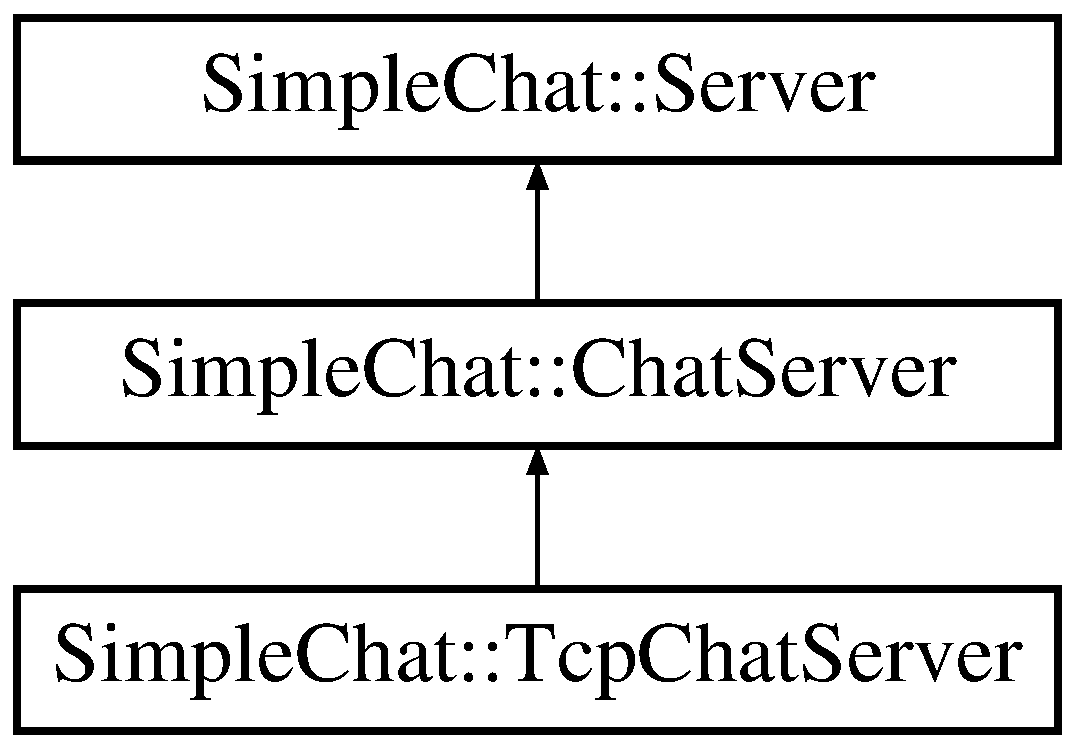
\includegraphics[height=3.000000cm]{classSimpleChat_1_1Server}
\end{center}
\end{figure}
\subsection*{Public Member Functions}
\begin{DoxyCompactItemize}
\item 
\hypertarget{classSimpleChat_1_1Server_a9e23c964082532000991ee2a2f699045}{virtual void {\bfseries chatee\-Left} (const std\-::shared\-\_\-ptr$<$ \hyperlink{classSimpleChat_1_1Chatee}{Chatee} $>$ \&chatee)=0}\label{classSimpleChat_1_1Server_a9e23c964082532000991ee2a2f699045}

\item 
\hypertarget{classSimpleChat_1_1Server_ad4b5157889b3d262efd3f86840aad333}{virtual void {\bfseries handle\-Untyped\-Message} (const \hyperlink{classSimpleChat_1_1MessageDeserializer}{Message\-Deserializer} \&deserializer, \hyperlink{classSimpleChat_1_1ChatConnection}{Chat\-Connection} $\ast$connection)=0}\label{classSimpleChat_1_1Server_ad4b5157889b3d262efd3f86840aad333}

\item 
\hypertarget{classSimpleChat_1_1Server_a73a8a4b05d7168c2b3b6213ccfc07c5e}{virtual void {\bfseries handle\-Message} (std\-::unique\-\_\-ptr$<$ \hyperlink{classSimpleChat_1_1UserJoinRequest}{User\-Join\-Request} $>$ join\-Request, \hyperlink{classSimpleChat_1_1ChatConnection}{Chat\-Connection} $\ast$connection)=0}\label{classSimpleChat_1_1Server_a73a8a4b05d7168c2b3b6213ccfc07c5e}

\item 
\hypertarget{classSimpleChat_1_1Server_a0826dd0d3d4f3f4c9cef8db37b3de0da}{virtual void {\bfseries handle\-Message} (std\-::unique\-\_\-ptr$<$ \hyperlink{classSimpleChat_1_1UserListRequest}{User\-List\-Request} $>$ list\-Request, const std\-::shared\-\_\-ptr$<$ \hyperlink{classSimpleChat_1_1Chatee}{Chatee} $>$ \&sender)=0}\label{classSimpleChat_1_1Server_a0826dd0d3d4f3f4c9cef8db37b3de0da}

\item 
\hypertarget{classSimpleChat_1_1Server_a41ee4829f9ec2726534ccdf47334b6d5}{virtual void {\bfseries handle\-Message} (std\-::unique\-\_\-ptr$<$ \hyperlink{classSimpleChat_1_1UserChange}{User\-Change} $>$ change, const std\-::shared\-\_\-ptr$<$ \hyperlink{classSimpleChat_1_1Chatee}{Chatee} $>$ \&sender)=0}\label{classSimpleChat_1_1Server_a41ee4829f9ec2726534ccdf47334b6d5}

\item 
\hypertarget{classSimpleChat_1_1Server_adbb31e147762d38576f1a959c65deff8}{virtual void {\bfseries handle\-Message} (std\-::unique\-\_\-ptr$<$ \hyperlink{classSimpleChat_1_1ChatMessage}{Chat\-Message} $>$ chat\-Message, const std\-::shared\-\_\-ptr$<$ \hyperlink{classSimpleChat_1_1Chatee}{Chatee} $>$ \&sender)=0}\label{classSimpleChat_1_1Server_adbb31e147762d38576f1a959c65deff8}

\item 
\hypertarget{classSimpleChat_1_1Server_a39468217b57290fc663b8874ac9fdf26}{virtual void {\bfseries handle\-Message} (std\-::unique\-\_\-ptr$<$ \hyperlink{classSimpleChat_1_1ChatCommand}{Chat\-Command} $>$ chat\-Command, const std\-::shared\-\_\-ptr$<$ \hyperlink{classSimpleChat_1_1Chatee}{Chatee} $>$ \&sender)=0}\label{classSimpleChat_1_1Server_a39468217b57290fc663b8874ac9fdf26}

\end{DoxyCompactItemize}


The documentation for this class was generated from the following file\-:\begin{DoxyCompactItemize}
\item 
chatlib/server/Server.\-h\end{DoxyCompactItemize}

\hypertarget{classSimpleChat_1_1SpecificChatCommand}{\section{Simple\-Chat\-:\-:Specific\-Chat\-Command Class Reference}
\label{classSimpleChat_1_1SpecificChatCommand}\index{Simple\-Chat\-::\-Specific\-Chat\-Command@{Simple\-Chat\-::\-Specific\-Chat\-Command}}
}
Inheritance diagram for Simple\-Chat\-:\-:Specific\-Chat\-Command\-:\begin{figure}[H]
\begin{center}
\leavevmode
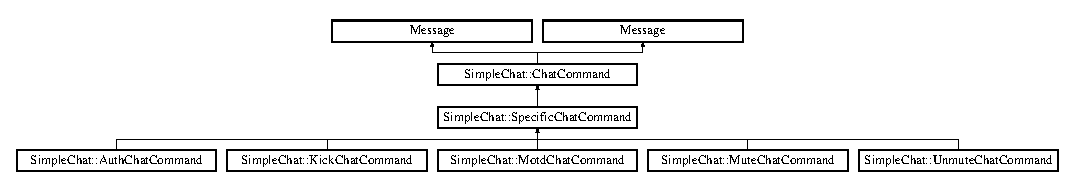
\includegraphics[height=2.074074cm]{classSimpleChat_1_1SpecificChatCommand}
\end{center}
\end{figure}
\subsection*{Public Member Functions}
\begin{DoxyCompactItemize}
\item 
\hypertarget{classSimpleChat_1_1SpecificChatCommand_a201ca79b92b4d5ad6ef78ddd39fc5aaa}{virtual void {\bfseries insert\-Data} (const std\-::vector$<$ std\-::string $>$ \&arguments)=0}\label{classSimpleChat_1_1SpecificChatCommand_a201ca79b92b4d5ad6ef78ddd39fc5aaa}

\end{DoxyCompactItemize}
\subsection*{Additional Inherited Members}


The documentation for this class was generated from the following file\-:\begin{DoxyCompactItemize}
\item 
chatlib/chat/commands/Specific\-Chat\-Command.\-h\end{DoxyCompactItemize}

\hypertarget{classSimpleChat_1_1TcpChatClient}{\section{Simple\-Chat\-:\-:Tcp\-Chat\-Client Class Reference}
\label{classSimpleChat_1_1TcpChatClient}\index{Simple\-Chat\-::\-Tcp\-Chat\-Client@{Simple\-Chat\-::\-Tcp\-Chat\-Client}}
}
Inheritance diagram for Simple\-Chat\-:\-:Tcp\-Chat\-Client\-:\begin{figure}[H]
\begin{center}
\leavevmode
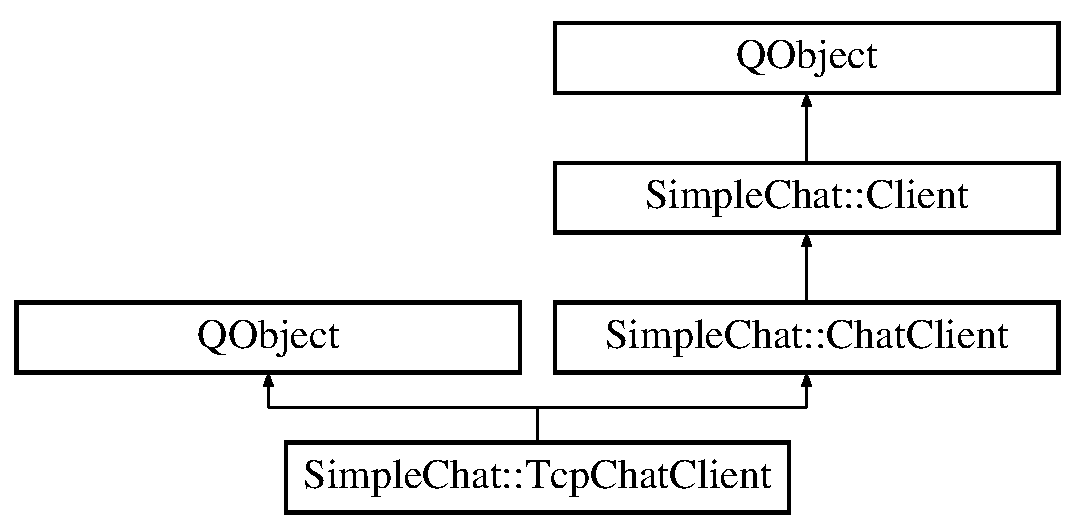
\includegraphics[height=4.000000cm]{classSimpleChat_1_1TcpChatClient}
\end{center}
\end{figure}
\subsection*{Signals}
\begin{DoxyCompactItemize}
\item 
\hypertarget{classSimpleChat_1_1TcpChatClient_ad227e90be4ba4c6c4ca05e6dc0f910ee}{void {\bfseries chatee\-Joined\-Signal} (const Q\-String \&name)}\label{classSimpleChat_1_1TcpChatClient_ad227e90be4ba4c6c4ca05e6dc0f910ee}

\item 
\hypertarget{classSimpleChat_1_1TcpChatClient_a9b92c990073439c47e147b3e6f2bfc2c}{void {\bfseries chatee\-Left\-Signal} (const Q\-String \&name)}\label{classSimpleChat_1_1TcpChatClient_a9b92c990073439c47e147b3e6f2bfc2c}

\item 
\hypertarget{classSimpleChat_1_1TcpChatClient_a361335d681dd4de2bb0b2ce4e34ff95f}{void {\bfseries chat\-Message\-Signal} (const Q\-String \&text, const Q\-String \&from, const Q\-String \&target)}\label{classSimpleChat_1_1TcpChatClient_a361335d681dd4de2bb0b2ce4e34ff95f}

\item 
\hypertarget{classSimpleChat_1_1TcpChatClient_a78428ed1c3f1dd6f9c28497c7f2bfa2a}{void {\bfseries chat\-Info\-Signal} (const Q\-String \&text)}\label{classSimpleChat_1_1TcpChatClient_a78428ed1c3f1dd6f9c28497c7f2bfa2a}

\item 
\hypertarget{classSimpleChat_1_1TcpChatClient_ae36b13ea9eaa5787c75f3f911e2afd68}{void {\bfseries chat\-Motd\-Signal} (const Q\-String \&motd)}\label{classSimpleChat_1_1TcpChatClient_ae36b13ea9eaa5787c75f3f911e2afd68}

\item 
\hypertarget{classSimpleChat_1_1TcpChatClient_a3d7860281a1ab069e5eaf367ba93b54d}{void {\bfseries chat\-Refresh\-List\-Signal} ()}\label{classSimpleChat_1_1TcpChatClient_a3d7860281a1ab069e5eaf367ba93b54d}

\end{DoxyCompactItemize}
\subsection*{Public Member Functions}
\begin{DoxyCompactItemize}
\item 
\hypertarget{classSimpleChat_1_1TcpChatClient_acd13e1bf8749dd0395e51ceabc7fdaf5}{{\bfseries Tcp\-Chat\-Client} (Q\-Object $\ast$parent=nullptr)}\label{classSimpleChat_1_1TcpChatClient_acd13e1bf8749dd0395e51ceabc7fdaf5}

\item 
\hypertarget{classSimpleChat_1_1TcpChatClient_a5f6302e6e92f8fc60721d5f042a2bd0a}{virtual bool {\bfseries login} (const Q\-String \&address, quint16 port, const Q\-String \&name)}\label{classSimpleChat_1_1TcpChatClient_a5f6302e6e92f8fc60721d5f042a2bd0a}

\item 
\hypertarget{classSimpleChat_1_1TcpChatClient_a7d582f1bee13aeaf77829fcdfef1cca4}{virtual void {\bfseries logout} ()}\label{classSimpleChat_1_1TcpChatClient_a7d582f1bee13aeaf77829fcdfef1cca4}

\item 
\hypertarget{classSimpleChat_1_1TcpChatClient_a4140c1693b4b675a4510f39ae51f593c}{virtual bool {\bfseries connect\-To\-Server} () override}\label{classSimpleChat_1_1TcpChatClient_a4140c1693b4b675a4510f39ae51f593c}

\item 
\hypertarget{classSimpleChat_1_1TcpChatClient_aef8015e0b6b273e671e7dcfd56dda837}{virtual void {\bfseries join} () override}\label{classSimpleChat_1_1TcpChatClient_aef8015e0b6b273e671e7dcfd56dda837}

\item 
\hypertarget{classSimpleChat_1_1TcpChatClient_abd27db3215c87dad68dbd2fd3c801ab8}{virtual void {\bfseries request\-User\-List} () override}\label{classSimpleChat_1_1TcpChatClient_abd27db3215c87dad68dbd2fd3c801ab8}

\end{DoxyCompactItemize}
\subsection*{Protected Member Functions}
\begin{DoxyCompactItemize}
\item 
\hypertarget{classSimpleChat_1_1TcpChatClient_ab2f4d6615bdb673a6f754aaff462a967}{virtual bool {\bfseries send\-Any\-Message} (std\-::unique\-\_\-ptr$<$ \hyperlink{classSimpleChat_1_1AbstractMessage}{Abstract\-Message} $>$ message) override}\label{classSimpleChat_1_1TcpChatClient_ab2f4d6615bdb673a6f754aaff462a967}

\item 
\hypertarget{classSimpleChat_1_1TcpChatClient_a05f4734c927c055a6c0a261d6639e55d}{virtual bool {\bfseries is\-Connected} () override}\label{classSimpleChat_1_1TcpChatClient_a05f4734c927c055a6c0a261d6639e55d}

\item 
\hypertarget{classSimpleChat_1_1TcpChatClient_a2ac493213fa789c77acc23b7e03ce535}{virtual \hyperlink{classSimpleChat_1_1ChatConnection}{Chat\-Connection} $\ast$ {\bfseries connection} () override}\label{classSimpleChat_1_1TcpChatClient_a2ac493213fa789c77acc23b7e03ce535}

\item 
\hypertarget{classSimpleChat_1_1TcpChatClient_abc3d3475944f9000fa37af0e74ef1eda}{virtual void {\bfseries chatee\-Joined} (const std\-::string \&name) override}\label{classSimpleChat_1_1TcpChatClient_abc3d3475944f9000fa37af0e74ef1eda}

\item 
\hypertarget{classSimpleChat_1_1TcpChatClient_a0ff71a80179c4d0306fc09ed4a475bcc}{virtual void {\bfseries chatee\-Left} (const std\-::string \&name) override}\label{classSimpleChat_1_1TcpChatClient_a0ff71a80179c4d0306fc09ed4a475bcc}

\item 
\hypertarget{classSimpleChat_1_1TcpChatClient_a1d62652f659ae0a4608ec90f86ac3fea}{virtual void {\bfseries chat\-Motd\-Changed} (const std\-::string \&motd) override}\label{classSimpleChat_1_1TcpChatClient_a1d62652f659ae0a4608ec90f86ac3fea}

\item 
\hypertarget{classSimpleChat_1_1TcpChatClient_a69db86b7aa3a140ad5d7ae108ae90668}{virtual void {\bfseries chat\-Info\-Received} (const std\-::string \&info) override}\label{classSimpleChat_1_1TcpChatClient_a69db86b7aa3a140ad5d7ae108ae90668}

\item 
\hypertarget{classSimpleChat_1_1TcpChatClient_ad554ab47a5e5b5876769af6cf3241665}{virtual void {\bfseries chat\-Message\-Received} (const std\-::string \&text, const std\-::string \&from, const std\-::string \&target) override}\label{classSimpleChat_1_1TcpChatClient_ad554ab47a5e5b5876769af6cf3241665}

\item 
\hypertarget{classSimpleChat_1_1TcpChatClient_a87835c8bcce725938c6dc470a8711232}{virtual void {\bfseries refresh\-Chatee\-List} () override}\label{classSimpleChat_1_1TcpChatClient_a87835c8bcce725938c6dc470a8711232}

\end{DoxyCompactItemize}
\subsection*{Additional Inherited Members}


The documentation for this class was generated from the following files\-:\begin{DoxyCompactItemize}
\item 
tcplib/client/Tcp\-Chat\-Client.\-h\item 
tcplib/client/Tcp\-Chat\-Client.\-cpp\item 
tcplib/moc\-\_\-\-Tcp\-Chat\-Client.\-cpp\end{DoxyCompactItemize}

\hypertarget{classSimpleChat_1_1TcpChatConnection}{\section{Simple\-Chat\-:\-:Tcp\-Chat\-Connection Class Reference}
\label{classSimpleChat_1_1TcpChatConnection}\index{Simple\-Chat\-::\-Tcp\-Chat\-Connection@{Simple\-Chat\-::\-Tcp\-Chat\-Connection}}
}
Inheritance diagram for Simple\-Chat\-:\-:Tcp\-Chat\-Connection\-:\begin{figure}[H]
\begin{center}
\leavevmode
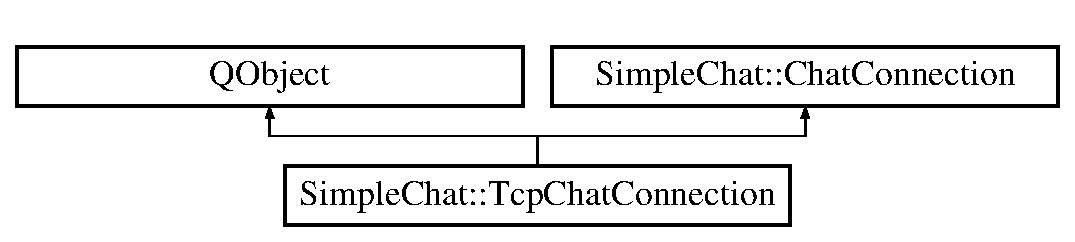
\includegraphics[height=2.000000cm]{classSimpleChat_1_1TcpChatConnection}
\end{center}
\end{figure}
\subsection*{Signals}
\begin{DoxyCompactItemize}
\item 
\hypertarget{classSimpleChat_1_1TcpChatConnection_acbd9d95bf1f80fd1c8325fb0e2d1655c}{void {\bfseries data\-Received\-Signal} (const Q\-String \&serialized\-Message)}\label{classSimpleChat_1_1TcpChatConnection_acbd9d95bf1f80fd1c8325fb0e2d1655c}

\item 
\hypertarget{classSimpleChat_1_1TcpChatConnection_a4950d5863fce3c72f8f0e4972b2f824f}{void {\bfseries disconnect\-Signal} ()}\label{classSimpleChat_1_1TcpChatConnection_a4950d5863fce3c72f8f0e4972b2f824f}

\end{DoxyCompactItemize}
\subsection*{Public Member Functions}
\begin{DoxyCompactItemize}
\item 
\hypertarget{classSimpleChat_1_1TcpChatConnection_a98eeb678c3851ecd89d9eaa42f2d4ed7}{{\bfseries Tcp\-Chat\-Connection} (Q\-Tcp\-Socket $\ast$socket, Q\-Object $\ast$parent=nullptr)}\label{classSimpleChat_1_1TcpChatConnection_a98eeb678c3851ecd89d9eaa42f2d4ed7}

\item 
\hypertarget{classSimpleChat_1_1TcpChatConnection_a4b67e948f1f6dbb1fedfc5c8f4995fac}{void {\bfseries init} () const }\label{classSimpleChat_1_1TcpChatConnection_a4b67e948f1f6dbb1fedfc5c8f4995fac}

\item 
\hypertarget{classSimpleChat_1_1TcpChatConnection_a70cf88d84909c6f541b5cafd23537f9b}{virtual bool {\bfseries send\-Message} (std\-::unique\-\_\-ptr$<$ \hyperlink{classSimpleChat_1_1AbstractMessage}{Abstract\-Message} $>$ message) override}\label{classSimpleChat_1_1TcpChatConnection_a70cf88d84909c6f541b5cafd23537f9b}

\item 
\hypertarget{classSimpleChat_1_1TcpChatConnection_a2765620a13f5fb7df8001829b01f1eb4}{virtual bool {\bfseries is\-Alive} () const override}\label{classSimpleChat_1_1TcpChatConnection_a2765620a13f5fb7df8001829b01f1eb4}

\item 
\hypertarget{classSimpleChat_1_1TcpChatConnection_a39c8ffddd847c0cf0942349e88143ff1}{virtual std\-::string {\bfseries get\-Ident} () const override}\label{classSimpleChat_1_1TcpChatConnection_a39c8ffddd847c0cf0942349e88143ff1}

\item 
\hypertarget{classSimpleChat_1_1TcpChatConnection_adfa72a80825262c93545627615dc62fd}{void {\bfseries disconnect\-From\-Host} () override}\label{classSimpleChat_1_1TcpChatConnection_adfa72a80825262c93545627615dc62fd}

\item 
\hypertarget{classSimpleChat_1_1TcpChatConnection_ab39fff987021e4d35f5ca3646e77f000}{virtual void {\bfseries set\-Chatee} (const std\-::shared\-\_\-ptr$<$ \hyperlink{classSimpleChat_1_1Chatee}{Chatee} $>$ \&chatee) override}\label{classSimpleChat_1_1TcpChatConnection_ab39fff987021e4d35f5ca3646e77f000}

\item 
\hypertarget{classSimpleChat_1_1TcpChatConnection_ae649c6797a93204f9383224b4c3d3160}{virtual std\-::shared\-\_\-ptr$<$ \hyperlink{classSimpleChat_1_1Chatee}{Chatee} $>$ {\bfseries chatee} () const override}\label{classSimpleChat_1_1TcpChatConnection_ae649c6797a93204f9383224b4c3d3160}

\item 
\hypertarget{classSimpleChat_1_1TcpChatConnection_a56c1b634770ba04677dd243f174c71fa}{Q\-Tcp\-Socket $\ast$ {\bfseries socket} () const }\label{classSimpleChat_1_1TcpChatConnection_a56c1b634770ba04677dd243f174c71fa}

\end{DoxyCompactItemize}


The documentation for this class was generated from the following files\-:\begin{DoxyCompactItemize}
\item 
tcplib/chat/Tcp\-Chat\-Connection.\-h\item 
tcplib/chat/Tcp\-Chat\-Connection.\-cpp\item 
tcplib/moc\-\_\-\-Tcp\-Chat\-Connection.\-cpp\end{DoxyCompactItemize}

\hypertarget{classSimpleChat_1_1TcpChatServer}{\section{Simple\-Chat\-:\-:Tcp\-Chat\-Server Class Reference}
\label{classSimpleChat_1_1TcpChatServer}\index{Simple\-Chat\-::\-Tcp\-Chat\-Server@{Simple\-Chat\-::\-Tcp\-Chat\-Server}}
}
Inheritance diagram for Simple\-Chat\-:\-:Tcp\-Chat\-Server\-:\begin{figure}[H]
\begin{center}
\leavevmode
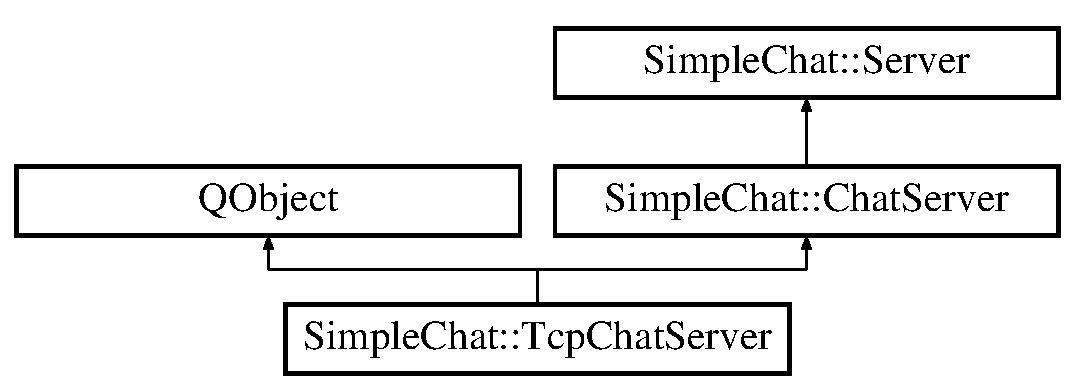
\includegraphics[height=3.000000cm]{classSimpleChat_1_1TcpChatServer}
\end{center}
\end{figure}
\subsection*{Public Member Functions}
\begin{DoxyCompactItemize}
\item 
\hypertarget{classSimpleChat_1_1TcpChatServer_a4d28d3a86626580c1d9761f570e1184f}{{\bfseries Tcp\-Chat\-Server} (const std\-::string \&password, Q\-Object $\ast$parent=nullptr)}\label{classSimpleChat_1_1TcpChatServer_a4d28d3a86626580c1d9761f570e1184f}

\item 
\hypertarget{classSimpleChat_1_1TcpChatServer_aecd09057f447d2a1f9882cbe319fa36a}{virtual void {\bfseries listen} (quint16 port, const Q\-Host\-Address \&ip\-Address)}\label{classSimpleChat_1_1TcpChatServer_aecd09057f447d2a1f9882cbe319fa36a}

\end{DoxyCompactItemize}
\subsection*{Additional Inherited Members}


The documentation for this class was generated from the following files\-:\begin{DoxyCompactItemize}
\item 
tcplib/server/Tcp\-Chat\-Server.\-h\item 
tcplib/server/Tcp\-Chat\-Server.\-cpp\end{DoxyCompactItemize}

\hypertarget{classUi__ChatDialog}{\section{Ui\-\_\-\-Chat\-Dialog Class Reference}
\label{classUi__ChatDialog}\index{Ui\-\_\-\-Chat\-Dialog@{Ui\-\_\-\-Chat\-Dialog}}
}
Inheritance diagram for Ui\-\_\-\-Chat\-Dialog\-:\begin{figure}[H]
\begin{center}
\leavevmode
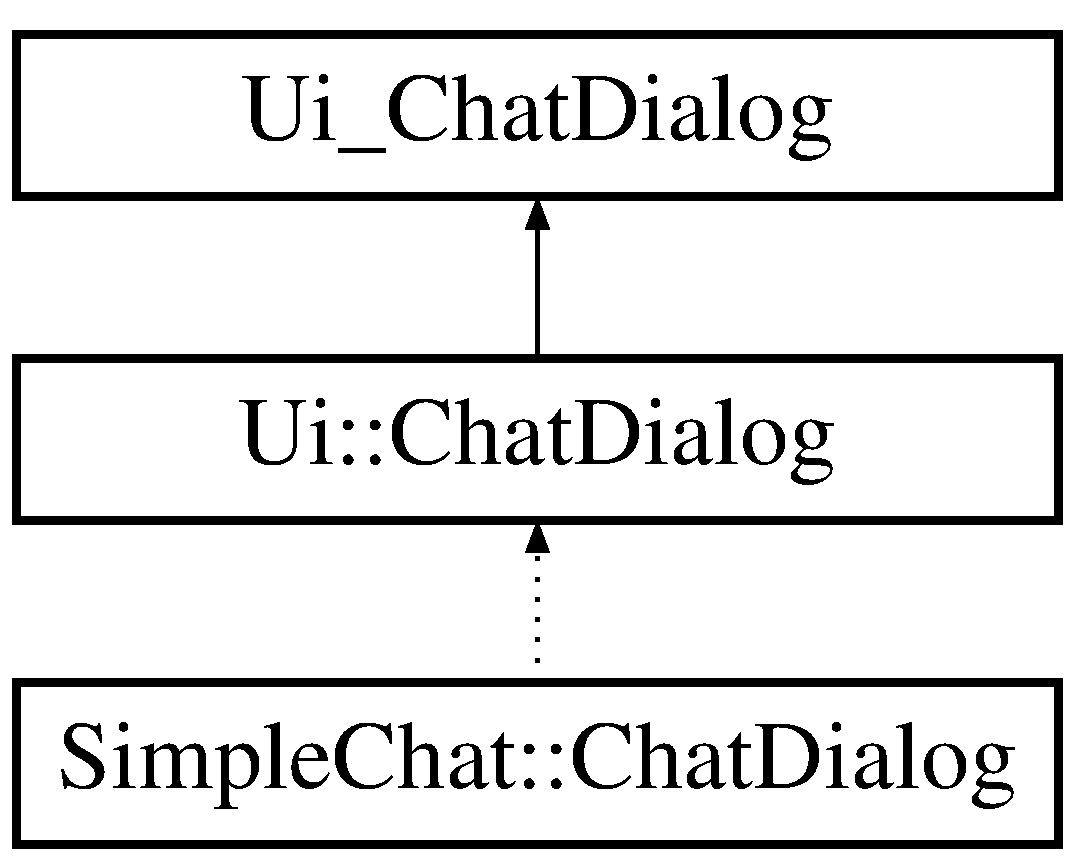
\includegraphics[height=3.000000cm]{classUi__ChatDialog}
\end{center}
\end{figure}
\subsection*{Public Member Functions}
\begin{DoxyCompactItemize}
\item 
\hypertarget{classUi__ChatDialog_ab8af0aca3bfb17111fb9992abba3519f}{void {\bfseries setup\-Ui} (Q\-Dialog $\ast$Chat\-Dialog)}\label{classUi__ChatDialog_ab8af0aca3bfb17111fb9992abba3519f}

\item 
\hypertarget{classUi__ChatDialog_a8a8431d8119a676a8f7712f34a72d6f2}{void {\bfseries retranslate\-Ui} (Q\-Dialog $\ast$Chat\-Dialog)}\label{classUi__ChatDialog_a8a8431d8119a676a8f7712f34a72d6f2}

\end{DoxyCompactItemize}
\subsection*{Public Attributes}
\begin{DoxyCompactItemize}
\item 
\hypertarget{classUi__ChatDialog_a42a613611496597c83e007a750b1c72b}{Q\-V\-Box\-Layout $\ast$ {\bfseries vbox\-Layout}}\label{classUi__ChatDialog_a42a613611496597c83e007a750b1c72b}

\item 
\hypertarget{classUi__ChatDialog_a4460c6a9ec5fde2262d323d16166c5c4}{Q\-H\-Box\-Layout $\ast$ {\bfseries hbox\-Layout}}\label{classUi__ChatDialog_a4460c6a9ec5fde2262d323d16166c5c4}

\item 
\hypertarget{classUi__ChatDialog_ab1b9ec11aae9e90b163c9d616facfb6a}{Q\-Text\-Edit $\ast$ {\bfseries text\-Edit}}\label{classUi__ChatDialog_ab1b9ec11aae9e90b163c9d616facfb6a}

\item 
\hypertarget{classUi__ChatDialog_a03367dcbea7a1a2488fa6c454cb519f9}{Q\-List\-Widget $\ast$ {\bfseries user\-List\-Widget}}\label{classUi__ChatDialog_a03367dcbea7a1a2488fa6c454cb519f9}

\item 
\hypertarget{classUi__ChatDialog_a2ee484e73ae8ff60547a2f795230b17e}{Q\-H\-Box\-Layout $\ast$ {\bfseries hbox\-Layout1}}\label{classUi__ChatDialog_a2ee484e73ae8ff60547a2f795230b17e}

\item 
\hypertarget{classUi__ChatDialog_a313c5bb54dac1c18cb5286d54c472aaa}{Q\-Label $\ast$ {\bfseries label}}\label{classUi__ChatDialog_a313c5bb54dac1c18cb5286d54c472aaa}

\item 
\hypertarget{classUi__ChatDialog_abc1ae793c0cd5652f9d7b7314d367c2b}{Q\-Line\-Edit $\ast$ {\bfseries line\-Edit}}\label{classUi__ChatDialog_abc1ae793c0cd5652f9d7b7314d367c2b}

\end{DoxyCompactItemize}


The documentation for this class was generated from the following file\-:\begin{DoxyCompactItemize}
\item 
client/ui\-\_\-chatdialog.\-h\end{DoxyCompactItemize}

\hypertarget{classSimpleChat_1_1UnmuteChatCommand}{\section{Simple\-Chat\-:\-:Unmute\-Chat\-Command Class Reference}
\label{classSimpleChat_1_1UnmuteChatCommand}\index{Simple\-Chat\-::\-Unmute\-Chat\-Command@{Simple\-Chat\-::\-Unmute\-Chat\-Command}}
}
Inheritance diagram for Simple\-Chat\-:\-:Unmute\-Chat\-Command\-:\begin{figure}[H]
\begin{center}
\leavevmode
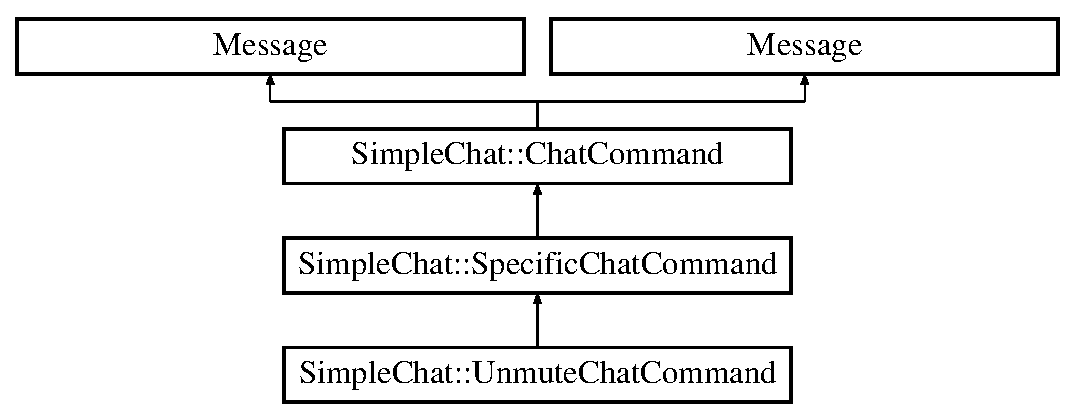
\includegraphics[height=4.000000cm]{classSimpleChat_1_1UnmuteChatCommand}
\end{center}
\end{figure}
\subsection*{Public Member Functions}
\begin{DoxyCompactItemize}
\item 
virtual void \hyperlink{classSimpleChat_1_1UnmuteChatCommand_a5e6fa7ebd1aae6f968c05d6934558bfa}{insert\-Data} (const std\-::vector$<$ std\-::string $>$ \&arguments) override
\end{DoxyCompactItemize}
\subsection*{Additional Inherited Members}


\subsection{Member Function Documentation}
\hypertarget{classSimpleChat_1_1UnmuteChatCommand_a5e6fa7ebd1aae6f968c05d6934558bfa}{\index{Simple\-Chat\-::\-Unmute\-Chat\-Command@{Simple\-Chat\-::\-Unmute\-Chat\-Command}!insert\-Data@{insert\-Data}}
\index{insert\-Data@{insert\-Data}!SimpleChat::UnmuteChatCommand@{Simple\-Chat\-::\-Unmute\-Chat\-Command}}
\subsubsection[{insert\-Data}]{\setlength{\rightskip}{0pt plus 5cm}void Simple\-Chat\-::\-Unmute\-Chat\-Command\-::insert\-Data (
\begin{DoxyParamCaption}
\item[{const std\-::vector$<$ std\-::string $>$ \&}]{arguments}
\end{DoxyParamCaption}
)\hspace{0.3cm}{\ttfamily [override]}, {\ttfamily [virtual]}}}\label{classSimpleChat_1_1UnmuteChatCommand_a5e6fa7ebd1aae6f968c05d6934558bfa}
argument is a name 

Implements \hyperlink{classSimpleChat_1_1SpecificChatCommand}{Simple\-Chat\-::\-Specific\-Chat\-Command}.



The documentation for this class was generated from the following files\-:\begin{DoxyCompactItemize}
\item 
chatlib/chat/commands/Unmute\-Chat\-Command.\-h\item 
chatlib/chat/commands/Unmute\-Chat\-Command.\-cpp\end{DoxyCompactItemize}

\hypertarget{classSimpleChat_1_1User}{\section{Simple\-Chat\-:\-:User Class Reference}
\label{classSimpleChat_1_1User}\index{Simple\-Chat\-::\-User@{Simple\-Chat\-::\-User}}
}
Inheritance diagram for Simple\-Chat\-:\-:User\-:\begin{figure}[H]
\begin{center}
\leavevmode
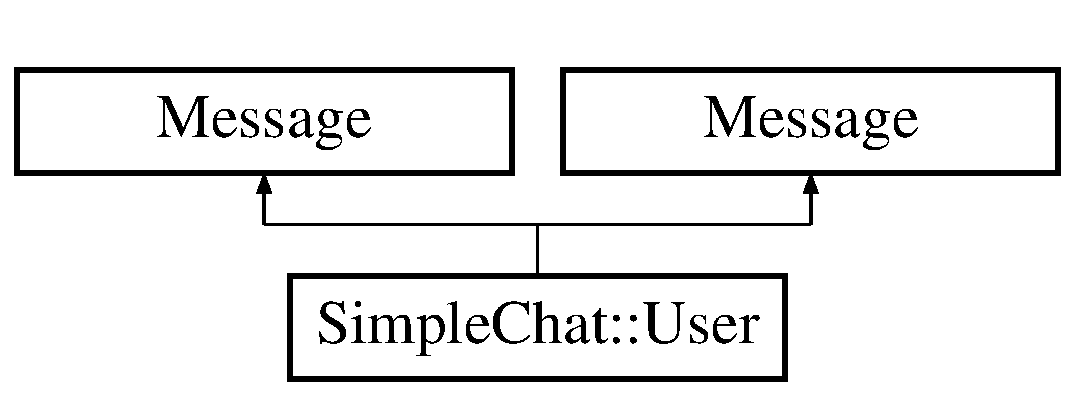
\includegraphics[height=2.000000cm]{classSimpleChat_1_1User}
\end{center}
\end{figure}
\subsection*{Public Member Functions}
\begin{DoxyCompactItemize}
\item 
\hypertarget{classSimpleChat_1_1User_af9d0c6966cc6131f24f689a2bb375562}{{\bfseries User} (const \hyperlink{classSimpleChat_1_1User}{User} \&from)}\label{classSimpleChat_1_1User_af9d0c6966cc6131f24f689a2bb375562}

\item 
\hypertarget{classSimpleChat_1_1User_aa62b1c0d29848bd524e819e174ea1b1d}{\hyperlink{classSimpleChat_1_1User}{User} \& {\bfseries operator=} (const \hyperlink{classSimpleChat_1_1User}{User} \&from)}\label{classSimpleChat_1_1User_aa62b1c0d29848bd524e819e174ea1b1d}

\item 
\hypertarget{classSimpleChat_1_1User_a74b47afc5050689cd12f8636d4a810cb}{const \\*
\-::google\-::protobuf\-::\-Unknown\-Field\-Set \& {\bfseries unknown\-\_\-fields} () const }\label{classSimpleChat_1_1User_a74b47afc5050689cd12f8636d4a810cb}

\item 
\hypertarget{classSimpleChat_1_1User_a89dd64bea6c553f3f803dab24a574acf}{inline\-::google\-::protobuf\-::\-Unknown\-Field\-Set $\ast$ {\bfseries mutable\-\_\-unknown\-\_\-fields} ()}\label{classSimpleChat_1_1User_a89dd64bea6c553f3f803dab24a574acf}

\item 
\hypertarget{classSimpleChat_1_1User_a7f64a6a4a7822d6a4d6dd8c3bc50132f}{void {\bfseries Swap} (\hyperlink{classSimpleChat_1_1User}{User} $\ast$other)}\label{classSimpleChat_1_1User_a7f64a6a4a7822d6a4d6dd8c3bc50132f}

\item 
\hypertarget{classSimpleChat_1_1User_ad6f7d285ea1db8b4d75de142f2b218e1}{\hyperlink{classSimpleChat_1_1User}{User} $\ast$ {\bfseries New} () const }\label{classSimpleChat_1_1User_ad6f7d285ea1db8b4d75de142f2b218e1}

\item 
\hypertarget{classSimpleChat_1_1User_ac6217a2abfe98ad2a6f2e15eee50d529}{\hyperlink{classSimpleChat_1_1User}{User} $\ast$ {\bfseries New} (\-::google\-::protobuf\-::\-Arena $\ast$arena) const }\label{classSimpleChat_1_1User_ac6217a2abfe98ad2a6f2e15eee50d529}

\item 
\hypertarget{classSimpleChat_1_1User_a867e04629c0c511b24a5da8c0449437c}{void {\bfseries Copy\-From} (const \-::google\-::protobuf\-::\-Message \&from)}\label{classSimpleChat_1_1User_a867e04629c0c511b24a5da8c0449437c}

\item 
\hypertarget{classSimpleChat_1_1User_aa98a5a27bfcb62c16a9481ad250b04e1}{void {\bfseries Merge\-From} (const \-::google\-::protobuf\-::\-Message \&from)}\label{classSimpleChat_1_1User_aa98a5a27bfcb62c16a9481ad250b04e1}

\item 
\hypertarget{classSimpleChat_1_1User_a0a68a82ad5773b1159f589ee7818473a}{void {\bfseries Copy\-From} (const \hyperlink{classSimpleChat_1_1User}{User} \&from)}\label{classSimpleChat_1_1User_a0a68a82ad5773b1159f589ee7818473a}

\item 
\hypertarget{classSimpleChat_1_1User_a4e808fbb7de9a513a82f4953f4570dab}{void {\bfseries Merge\-From} (const \hyperlink{classSimpleChat_1_1User}{User} \&from)}\label{classSimpleChat_1_1User_a4e808fbb7de9a513a82f4953f4570dab}

\item 
\hypertarget{classSimpleChat_1_1User_a9f4642144eddd10efeea8ebaff51ca65}{void {\bfseries Clear} ()}\label{classSimpleChat_1_1User_a9f4642144eddd10efeea8ebaff51ca65}

\item 
\hypertarget{classSimpleChat_1_1User_a8297129a543c5ca7b463c4ba4c068894}{bool {\bfseries Is\-Initialized} () const }\label{classSimpleChat_1_1User_a8297129a543c5ca7b463c4ba4c068894}

\item 
\hypertarget{classSimpleChat_1_1User_a43b778242ccd21d5d75bd4dc081be929}{int {\bfseries Byte\-Size} () const }\label{classSimpleChat_1_1User_a43b778242ccd21d5d75bd4dc081be929}

\item 
\hypertarget{classSimpleChat_1_1User_a4059958ebf9d50ce6acc096d61ff77b7}{bool {\bfseries Merge\-Partial\-From\-Coded\-Stream} (\-::google\-::protobuf\-::io\-::\-Coded\-Input\-Stream $\ast$input)}\label{classSimpleChat_1_1User_a4059958ebf9d50ce6acc096d61ff77b7}

\item 
\hypertarget{classSimpleChat_1_1User_af2d83f1ae710a5641e6cc163c81c0a3e}{void {\bfseries Serialize\-With\-Cached\-Sizes} (\-::google\-::protobuf\-::io\-::\-Coded\-Output\-Stream $\ast$output) const }\label{classSimpleChat_1_1User_af2d83f1ae710a5641e6cc163c81c0a3e}

\item 
\hypertarget{classSimpleChat_1_1User_a3cc508253897c0ea00a617065d24b9a4}{\-::google\-::protobuf\-::uint8 $\ast$ {\bfseries Serialize\-With\-Cached\-Sizes\-To\-Array} (\-::google\-::protobuf\-::uint8 $\ast$output) const }\label{classSimpleChat_1_1User_a3cc508253897c0ea00a617065d24b9a4}

\item 
\hypertarget{classSimpleChat_1_1User_abf5060695e86b14ca602e7453fc95360}{int {\bfseries Get\-Cached\-Size} () const }\label{classSimpleChat_1_1User_abf5060695e86b14ca602e7453fc95360}

\item 
\hypertarget{classSimpleChat_1_1User_a56cdcadf584c69e52f1bb8913b067940}{\-::google\-::protobuf\-::\-Metadata {\bfseries Get\-Metadata} () const }\label{classSimpleChat_1_1User_a56cdcadf584c69e52f1bb8913b067940}

\item 
\hypertarget{classSimpleChat_1_1User_ae369bb25f05d002d445fc7d244d78841}{bool {\bfseries has\-\_\-id} () const }\label{classSimpleChat_1_1User_ae369bb25f05d002d445fc7d244d78841}

\item 
\hypertarget{classSimpleChat_1_1User_ac7977c56651293b1efd5bbea639a45ce}{void {\bfseries clear\-\_\-id} ()}\label{classSimpleChat_1_1User_ac7977c56651293b1efd5bbea639a45ce}

\item 
\hypertarget{classSimpleChat_1_1User_aaa41321499ba3bc60f8d0df0acabde32}{\-::google\-::protobuf\-::int32 {\bfseries id} () const }\label{classSimpleChat_1_1User_aaa41321499ba3bc60f8d0df0acabde32}

\item 
\hypertarget{classSimpleChat_1_1User_a42e7249ccc18c7d421a00c4560c7d6e3}{void {\bfseries set\-\_\-id} (\-::google\-::protobuf\-::int32 value)}\label{classSimpleChat_1_1User_a42e7249ccc18c7d421a00c4560c7d6e3}

\item 
\hypertarget{classSimpleChat_1_1User_a4fa8407eb36f302de9afeb58670202c0}{bool {\bfseries has\-\_\-name} () const }\label{classSimpleChat_1_1User_a4fa8407eb36f302de9afeb58670202c0}

\item 
\hypertarget{classSimpleChat_1_1User_a4d9132c14159dcd3484f2e66a460338d}{void {\bfseries clear\-\_\-name} ()}\label{classSimpleChat_1_1User_a4d9132c14159dcd3484f2e66a460338d}

\item 
\hypertarget{classSimpleChat_1_1User_a8c1951e1c1b3600ca2c6936e7f210521}{const \-::std\-::string \& {\bfseries name} () const }\label{classSimpleChat_1_1User_a8c1951e1c1b3600ca2c6936e7f210521}

\item 
\hypertarget{classSimpleChat_1_1User_aad7063635c8f76c6cb7a5d39f9968d12}{void {\bfseries set\-\_\-name} (const \-::std\-::string \&value)}\label{classSimpleChat_1_1User_aad7063635c8f76c6cb7a5d39f9968d12}

\item 
\hypertarget{classSimpleChat_1_1User_af35ec09383b0f6d08c9e7b3504e390e0}{void {\bfseries set\-\_\-name} (const char $\ast$value)}\label{classSimpleChat_1_1User_af35ec09383b0f6d08c9e7b3504e390e0}

\item 
\hypertarget{classSimpleChat_1_1User_a1359df9c2b899976cf1009decfece340}{void {\bfseries set\-\_\-name} (const char $\ast$value, size\-\_\-t size)}\label{classSimpleChat_1_1User_a1359df9c2b899976cf1009decfece340}

\item 
\hypertarget{classSimpleChat_1_1User_a742405a8109ee29dffcf727033cdb663}{\-::std\-::string $\ast$ {\bfseries mutable\-\_\-name} ()}\label{classSimpleChat_1_1User_a742405a8109ee29dffcf727033cdb663}

\item 
\hypertarget{classSimpleChat_1_1User_a448d43306fd147672063875ab30a12ee}{\-::std\-::string $\ast$ {\bfseries release\-\_\-name} ()}\label{classSimpleChat_1_1User_a448d43306fd147672063875ab30a12ee}

\item 
\hypertarget{classSimpleChat_1_1User_a9d4774e5abe7bba7e01065344cb94ab5}{void {\bfseries set\-\_\-allocated\-\_\-name} (\-::std\-::string $\ast$name)}\label{classSimpleChat_1_1User_a9d4774e5abe7bba7e01065344cb94ab5}

\item 
\hypertarget{classSimpleChat_1_1User_a3696c71b8ac996eba4e1ed2cfc5128f4}{bool {\bfseries has\-\_\-presence} () const }\label{classSimpleChat_1_1User_a3696c71b8ac996eba4e1ed2cfc5128f4}

\item 
\hypertarget{classSimpleChat_1_1User_af810ab7c99299a594cd01ea507691835}{void {\bfseries clear\-\_\-presence} ()}\label{classSimpleChat_1_1User_af810ab7c99299a594cd01ea507691835}

\item 
\hypertarget{classSimpleChat_1_1User_a4310d4da92fee0889e90e5939e59dd4a}{\-::Simple\-Chat\-::\-User\-Presence {\bfseries presence} () const }\label{classSimpleChat_1_1User_a4310d4da92fee0889e90e5939e59dd4a}

\item 
\hypertarget{classSimpleChat_1_1User_abce18e8edb234ff2720525d9648377f1}{void {\bfseries set\-\_\-presence} (\-::Simple\-Chat\-::\-User\-Presence value)}\label{classSimpleChat_1_1User_abce18e8edb234ff2720525d9648377f1}

\item 
\hypertarget{classSimpleChat_1_1User_ac9ba533a79223fc1c8115d3464cc8e5e}{bool {\bfseries has\-\_\-mute} () const }\label{classSimpleChat_1_1User_ac9ba533a79223fc1c8115d3464cc8e5e}

\item 
\hypertarget{classSimpleChat_1_1User_ac0ae8cf95c70f0feae09dca283731d0a}{void {\bfseries clear\-\_\-mute} ()}\label{classSimpleChat_1_1User_ac0ae8cf95c70f0feae09dca283731d0a}

\item 
\hypertarget{classSimpleChat_1_1User_a5ee0fca06bd244943d6df037061cbe65}{bool {\bfseries mute} () const }\label{classSimpleChat_1_1User_a5ee0fca06bd244943d6df037061cbe65}

\item 
\hypertarget{classSimpleChat_1_1User_acfc6dcd5e75e732aada78bc551417d65}{void {\bfseries set\-\_\-mute} (bool value)}\label{classSimpleChat_1_1User_acfc6dcd5e75e732aada78bc551417d65}

\item 
\hypertarget{classSimpleChat_1_1User_af9d0c6966cc6131f24f689a2bb375562}{{\bfseries User} (const \hyperlink{classSimpleChat_1_1User}{User} \&from)}\label{classSimpleChat_1_1User_af9d0c6966cc6131f24f689a2bb375562}

\item 
\hypertarget{classSimpleChat_1_1User_aa62b1c0d29848bd524e819e174ea1b1d}{\hyperlink{classSimpleChat_1_1User}{User} \& {\bfseries operator=} (const \hyperlink{classSimpleChat_1_1User}{User} \&from)}\label{classSimpleChat_1_1User_aa62b1c0d29848bd524e819e174ea1b1d}

\item 
\hypertarget{classSimpleChat_1_1User_a74b47afc5050689cd12f8636d4a810cb}{const \\*
\-::google\-::protobuf\-::\-Unknown\-Field\-Set \& {\bfseries unknown\-\_\-fields} () const }\label{classSimpleChat_1_1User_a74b47afc5050689cd12f8636d4a810cb}

\item 
\hypertarget{classSimpleChat_1_1User_a89dd64bea6c553f3f803dab24a574acf}{inline\-::google\-::protobuf\-::\-Unknown\-Field\-Set $\ast$ {\bfseries mutable\-\_\-unknown\-\_\-fields} ()}\label{classSimpleChat_1_1User_a89dd64bea6c553f3f803dab24a574acf}

\item 
\hypertarget{classSimpleChat_1_1User_a7f64a6a4a7822d6a4d6dd8c3bc50132f}{void {\bfseries Swap} (\hyperlink{classSimpleChat_1_1User}{User} $\ast$other)}\label{classSimpleChat_1_1User_a7f64a6a4a7822d6a4d6dd8c3bc50132f}

\item 
\hypertarget{classSimpleChat_1_1User_ad6f7d285ea1db8b4d75de142f2b218e1}{\hyperlink{classSimpleChat_1_1User}{User} $\ast$ {\bfseries New} () const }\label{classSimpleChat_1_1User_ad6f7d285ea1db8b4d75de142f2b218e1}

\item 
\hypertarget{classSimpleChat_1_1User_ac6217a2abfe98ad2a6f2e15eee50d529}{\hyperlink{classSimpleChat_1_1User}{User} $\ast$ {\bfseries New} (\-::google\-::protobuf\-::\-Arena $\ast$arena) const }\label{classSimpleChat_1_1User_ac6217a2abfe98ad2a6f2e15eee50d529}

\item 
\hypertarget{classSimpleChat_1_1User_a867e04629c0c511b24a5da8c0449437c}{void {\bfseries Copy\-From} (const \-::google\-::protobuf\-::\-Message \&from)}\label{classSimpleChat_1_1User_a867e04629c0c511b24a5da8c0449437c}

\item 
\hypertarget{classSimpleChat_1_1User_aa98a5a27bfcb62c16a9481ad250b04e1}{void {\bfseries Merge\-From} (const \-::google\-::protobuf\-::\-Message \&from)}\label{classSimpleChat_1_1User_aa98a5a27bfcb62c16a9481ad250b04e1}

\item 
\hypertarget{classSimpleChat_1_1User_a0a68a82ad5773b1159f589ee7818473a}{void {\bfseries Copy\-From} (const \hyperlink{classSimpleChat_1_1User}{User} \&from)}\label{classSimpleChat_1_1User_a0a68a82ad5773b1159f589ee7818473a}

\item 
\hypertarget{classSimpleChat_1_1User_a4e808fbb7de9a513a82f4953f4570dab}{void {\bfseries Merge\-From} (const \hyperlink{classSimpleChat_1_1User}{User} \&from)}\label{classSimpleChat_1_1User_a4e808fbb7de9a513a82f4953f4570dab}

\item 
\hypertarget{classSimpleChat_1_1User_a9f4642144eddd10efeea8ebaff51ca65}{void {\bfseries Clear} ()}\label{classSimpleChat_1_1User_a9f4642144eddd10efeea8ebaff51ca65}

\item 
\hypertarget{classSimpleChat_1_1User_a8297129a543c5ca7b463c4ba4c068894}{bool {\bfseries Is\-Initialized} () const }\label{classSimpleChat_1_1User_a8297129a543c5ca7b463c4ba4c068894}

\item 
\hypertarget{classSimpleChat_1_1User_a43b778242ccd21d5d75bd4dc081be929}{int {\bfseries Byte\-Size} () const }\label{classSimpleChat_1_1User_a43b778242ccd21d5d75bd4dc081be929}

\item 
\hypertarget{classSimpleChat_1_1User_a4059958ebf9d50ce6acc096d61ff77b7}{bool {\bfseries Merge\-Partial\-From\-Coded\-Stream} (\-::google\-::protobuf\-::io\-::\-Coded\-Input\-Stream $\ast$input)}\label{classSimpleChat_1_1User_a4059958ebf9d50ce6acc096d61ff77b7}

\item 
\hypertarget{classSimpleChat_1_1User_af2d83f1ae710a5641e6cc163c81c0a3e}{void {\bfseries Serialize\-With\-Cached\-Sizes} (\-::google\-::protobuf\-::io\-::\-Coded\-Output\-Stream $\ast$output) const }\label{classSimpleChat_1_1User_af2d83f1ae710a5641e6cc163c81c0a3e}

\item 
\hypertarget{classSimpleChat_1_1User_a3cc508253897c0ea00a617065d24b9a4}{\-::google\-::protobuf\-::uint8 $\ast$ {\bfseries Serialize\-With\-Cached\-Sizes\-To\-Array} (\-::google\-::protobuf\-::uint8 $\ast$output) const }\label{classSimpleChat_1_1User_a3cc508253897c0ea00a617065d24b9a4}

\item 
\hypertarget{classSimpleChat_1_1User_abf5060695e86b14ca602e7453fc95360}{int {\bfseries Get\-Cached\-Size} () const }\label{classSimpleChat_1_1User_abf5060695e86b14ca602e7453fc95360}

\item 
\hypertarget{classSimpleChat_1_1User_a56cdcadf584c69e52f1bb8913b067940}{\-::google\-::protobuf\-::\-Metadata {\bfseries Get\-Metadata} () const }\label{classSimpleChat_1_1User_a56cdcadf584c69e52f1bb8913b067940}

\item 
\hypertarget{classSimpleChat_1_1User_ae369bb25f05d002d445fc7d244d78841}{bool {\bfseries has\-\_\-id} () const }\label{classSimpleChat_1_1User_ae369bb25f05d002d445fc7d244d78841}

\item 
\hypertarget{classSimpleChat_1_1User_ac7977c56651293b1efd5bbea639a45ce}{void {\bfseries clear\-\_\-id} ()}\label{classSimpleChat_1_1User_ac7977c56651293b1efd5bbea639a45ce}

\item 
\hypertarget{classSimpleChat_1_1User_aebeb2f5336d6a553e090dd0e3cbfcbab}{\-::google\-::protobuf\-::int32 {\bfseries id} () const }\label{classSimpleChat_1_1User_aebeb2f5336d6a553e090dd0e3cbfcbab}

\item 
\hypertarget{classSimpleChat_1_1User_a42e7249ccc18c7d421a00c4560c7d6e3}{void {\bfseries set\-\_\-id} (\-::google\-::protobuf\-::int32 value)}\label{classSimpleChat_1_1User_a42e7249ccc18c7d421a00c4560c7d6e3}

\item 
\hypertarget{classSimpleChat_1_1User_a4fa8407eb36f302de9afeb58670202c0}{bool {\bfseries has\-\_\-name} () const }\label{classSimpleChat_1_1User_a4fa8407eb36f302de9afeb58670202c0}

\item 
\hypertarget{classSimpleChat_1_1User_a4d9132c14159dcd3484f2e66a460338d}{void {\bfseries clear\-\_\-name} ()}\label{classSimpleChat_1_1User_a4d9132c14159dcd3484f2e66a460338d}

\item 
\hypertarget{classSimpleChat_1_1User_a06790ad4fc48a7d2a4ea96bc5f577c8e}{const \-::std\-::string \& {\bfseries name} () const }\label{classSimpleChat_1_1User_a06790ad4fc48a7d2a4ea96bc5f577c8e}

\item 
\hypertarget{classSimpleChat_1_1User_aad7063635c8f76c6cb7a5d39f9968d12}{void {\bfseries set\-\_\-name} (const \-::std\-::string \&value)}\label{classSimpleChat_1_1User_aad7063635c8f76c6cb7a5d39f9968d12}

\item 
\hypertarget{classSimpleChat_1_1User_af35ec09383b0f6d08c9e7b3504e390e0}{void {\bfseries set\-\_\-name} (const char $\ast$value)}\label{classSimpleChat_1_1User_af35ec09383b0f6d08c9e7b3504e390e0}

\item 
\hypertarget{classSimpleChat_1_1User_a1359df9c2b899976cf1009decfece340}{void {\bfseries set\-\_\-name} (const char $\ast$value, size\-\_\-t size)}\label{classSimpleChat_1_1User_a1359df9c2b899976cf1009decfece340}

\item 
\hypertarget{classSimpleChat_1_1User_a0ffb1fb69382e17472fd5ce9351f43d9}{\-::std\-::string $\ast$ {\bfseries mutable\-\_\-name} ()}\label{classSimpleChat_1_1User_a0ffb1fb69382e17472fd5ce9351f43d9}

\item 
\hypertarget{classSimpleChat_1_1User_ae0bddaa2e6fface79b47b98bb44192d4}{\-::std\-::string $\ast$ {\bfseries release\-\_\-name} ()}\label{classSimpleChat_1_1User_ae0bddaa2e6fface79b47b98bb44192d4}

\item 
\hypertarget{classSimpleChat_1_1User_a9d4774e5abe7bba7e01065344cb94ab5}{void {\bfseries set\-\_\-allocated\-\_\-name} (\-::std\-::string $\ast$name)}\label{classSimpleChat_1_1User_a9d4774e5abe7bba7e01065344cb94ab5}

\item 
\hypertarget{classSimpleChat_1_1User_a3696c71b8ac996eba4e1ed2cfc5128f4}{bool {\bfseries has\-\_\-presence} () const }\label{classSimpleChat_1_1User_a3696c71b8ac996eba4e1ed2cfc5128f4}

\item 
\hypertarget{classSimpleChat_1_1User_af810ab7c99299a594cd01ea507691835}{void {\bfseries clear\-\_\-presence} ()}\label{classSimpleChat_1_1User_af810ab7c99299a594cd01ea507691835}

\item 
\hypertarget{classSimpleChat_1_1User_a381ff8f5de1705967badcbd4d67d969b}{\-::Simple\-Chat\-::\-User\-Presence {\bfseries presence} () const }\label{classSimpleChat_1_1User_a381ff8f5de1705967badcbd4d67d969b}

\item 
\hypertarget{classSimpleChat_1_1User_abce18e8edb234ff2720525d9648377f1}{void {\bfseries set\-\_\-presence} (\-::Simple\-Chat\-::\-User\-Presence value)}\label{classSimpleChat_1_1User_abce18e8edb234ff2720525d9648377f1}

\item 
\hypertarget{classSimpleChat_1_1User_a0d3fabf6fe4fdb07bf490de3532f4853}{bool {\bfseries has\-\_\-status} () const }\label{classSimpleChat_1_1User_a0d3fabf6fe4fdb07bf490de3532f4853}

\item 
\hypertarget{classSimpleChat_1_1User_a50472728102691f22a1908831566956e}{void {\bfseries clear\-\_\-status} ()}\label{classSimpleChat_1_1User_a50472728102691f22a1908831566956e}

\item 
\hypertarget{classSimpleChat_1_1User_a0d7fc30246e8605a32a1cbaef5055a49}{\-::Simple\-Chat\-::\-User\-Status {\bfseries status} () const }\label{classSimpleChat_1_1User_a0d7fc30246e8605a32a1cbaef5055a49}

\item 
\hypertarget{classSimpleChat_1_1User_a6da4a04d2a3ac63b5d389a1ab4cb53c6}{void {\bfseries set\-\_\-status} (\-::Simple\-Chat\-::\-User\-Status value)}\label{classSimpleChat_1_1User_a6da4a04d2a3ac63b5d389a1ab4cb53c6}

\end{DoxyCompactItemize}
\subsection*{Static Public Member Functions}
\begin{DoxyCompactItemize}
\item 
\hypertarget{classSimpleChat_1_1User_a56f56187e04d8b7b4731712769255af2}{static const \\*
\-::google\-::protobuf\-::\-Descriptor $\ast$ {\bfseries descriptor} ()}\label{classSimpleChat_1_1User_a56f56187e04d8b7b4731712769255af2}

\item 
\hypertarget{classSimpleChat_1_1User_ae3104aea0a851e8ce14d98f2302c1453}{static const \hyperlink{classSimpleChat_1_1User}{User} \& {\bfseries default\-\_\-instance} ()}\label{classSimpleChat_1_1User_ae3104aea0a851e8ce14d98f2302c1453}

\item 
\hypertarget{classSimpleChat_1_1User_a56f56187e04d8b7b4731712769255af2}{static const \\*
\-::google\-::protobuf\-::\-Descriptor $\ast$ {\bfseries descriptor} ()}\label{classSimpleChat_1_1User_a56f56187e04d8b7b4731712769255af2}

\item 
\hypertarget{classSimpleChat_1_1User_ae3104aea0a851e8ce14d98f2302c1453}{static const \hyperlink{classSimpleChat_1_1User}{User} \& {\bfseries default\-\_\-instance} ()}\label{classSimpleChat_1_1User_ae3104aea0a851e8ce14d98f2302c1453}

\end{DoxyCompactItemize}
\subsection*{Static Public Attributes}
\begin{DoxyCompactItemize}
\item 
\hypertarget{classSimpleChat_1_1User_add8dabbd4cc64cf9bcbb0d64d2e7c18c}{static const int {\bfseries k\-Id\-Field\-Number} = 1}\label{classSimpleChat_1_1User_add8dabbd4cc64cf9bcbb0d64d2e7c18c}

\item 
\hypertarget{classSimpleChat_1_1User_aff843866ad3c9041af98dd7fe22274af}{static const int {\bfseries k\-Name\-Field\-Number} = 2}\label{classSimpleChat_1_1User_aff843866ad3c9041af98dd7fe22274af}

\item 
\hypertarget{classSimpleChat_1_1User_ac514bbc5ec69701baccb473d41f11d93}{static const int {\bfseries k\-Presence\-Field\-Number} = 3}\label{classSimpleChat_1_1User_ac514bbc5ec69701baccb473d41f11d93}

\item 
\hypertarget{classSimpleChat_1_1User_a70dc40535f467c770ba9a744e70f9138}{static const int {\bfseries k\-Mute\-Field\-Number} = 4}\label{classSimpleChat_1_1User_a70dc40535f467c770ba9a744e70f9138}

\item 
\hypertarget{classSimpleChat_1_1User_aad7c594d0c8d4e503478edcb6aa6ff84}{static const int {\bfseries k\-Status\-Field\-Number} = 4}\label{classSimpleChat_1_1User_aad7c594d0c8d4e503478edcb6aa6ff84}

\end{DoxyCompactItemize}
\subsection*{Friends}
\begin{DoxyCompactItemize}
\item 
\hypertarget{classSimpleChat_1_1User_a21c725e9955d4dda1abc79b117f57e76}{void {\bfseries protobuf\-\_\-\-Add\-Desc\-\_\-\-User\-\_\-2eproto} ()}\label{classSimpleChat_1_1User_a21c725e9955d4dda1abc79b117f57e76}

\item 
\hypertarget{classSimpleChat_1_1User_aadc83181f80ae5102c4449a54aef288e}{void {\bfseries protobuf\-\_\-\-Assign\-Desc\-\_\-\-User\-\_\-2eproto} ()}\label{classSimpleChat_1_1User_aadc83181f80ae5102c4449a54aef288e}

\item 
\hypertarget{classSimpleChat_1_1User_ac6d6bd3817a5978496745d793da7465f}{void {\bfseries protobuf\-\_\-\-Shutdown\-File\-\_\-\-User\-\_\-2eproto} ()}\label{classSimpleChat_1_1User_ac6d6bd3817a5978496745d793da7465f}

\item 
\hypertarget{classSimpleChat_1_1User_a21c725e9955d4dda1abc79b117f57e76}{void {\bfseries protobuf\-\_\-\-Add\-Desc\-\_\-\-User\-\_\-2eproto} ()}\label{classSimpleChat_1_1User_a21c725e9955d4dda1abc79b117f57e76}

\item 
\hypertarget{classSimpleChat_1_1User_aadc83181f80ae5102c4449a54aef288e}{void {\bfseries protobuf\-\_\-\-Assign\-Desc\-\_\-\-User\-\_\-2eproto} ()}\label{classSimpleChat_1_1User_aadc83181f80ae5102c4449a54aef288e}

\item 
\hypertarget{classSimpleChat_1_1User_ac6d6bd3817a5978496745d793da7465f}{void {\bfseries protobuf\-\_\-\-Shutdown\-File\-\_\-\-User\-\_\-2eproto} ()}\label{classSimpleChat_1_1User_ac6d6bd3817a5978496745d793da7465f}

\end{DoxyCompactItemize}


The documentation for this class was generated from the following file\-:\begin{DoxyCompactItemize}
\item 
chatlib/proto/User.\-pb.\-h\end{DoxyCompactItemize}

\hypertarget{classSimpleChat_1_1UserChange}{\section{Simple\-Chat\-:\-:User\-Change Class Reference}
\label{classSimpleChat_1_1UserChange}\index{Simple\-Chat\-::\-User\-Change@{Simple\-Chat\-::\-User\-Change}}
}
Inheritance diagram for Simple\-Chat\-:\-:User\-Change\-:\begin{figure}[H]
\begin{center}
\leavevmode
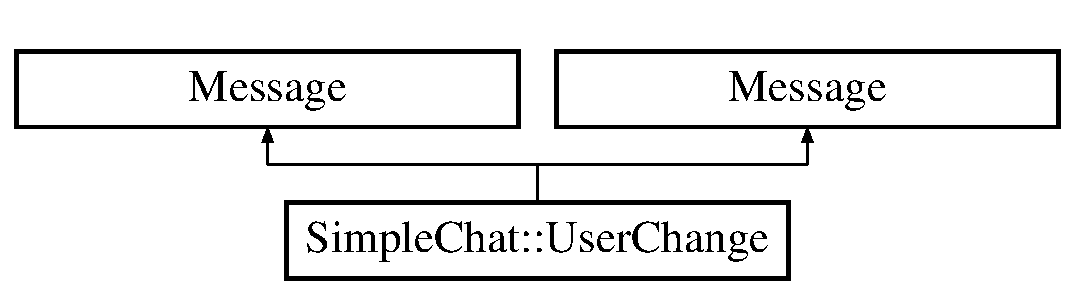
\includegraphics[height=2.000000cm]{classSimpleChat_1_1UserChange}
\end{center}
\end{figure}
\subsection*{Public Member Functions}
\begin{DoxyCompactItemize}
\item 
\hypertarget{classSimpleChat_1_1UserChange_a98ca1ff874642317f5f0ac5e1ae2dc30}{{\bfseries User\-Change} (const \hyperlink{classSimpleChat_1_1UserChange}{User\-Change} \&from)}\label{classSimpleChat_1_1UserChange_a98ca1ff874642317f5f0ac5e1ae2dc30}

\item 
\hypertarget{classSimpleChat_1_1UserChange_ad391b41999e61260da05e2d8b3c8635f}{\hyperlink{classSimpleChat_1_1UserChange}{User\-Change} \& {\bfseries operator=} (const \hyperlink{classSimpleChat_1_1UserChange}{User\-Change} \&from)}\label{classSimpleChat_1_1UserChange_ad391b41999e61260da05e2d8b3c8635f}

\item 
\hypertarget{classSimpleChat_1_1UserChange_ab1379a1c02c0fc0c33c8ffc8c070ed7f}{const \\*
\-::google\-::protobuf\-::\-Unknown\-Field\-Set \& {\bfseries unknown\-\_\-fields} () const }\label{classSimpleChat_1_1UserChange_ab1379a1c02c0fc0c33c8ffc8c070ed7f}

\item 
\hypertarget{classSimpleChat_1_1UserChange_a41d734c4dd617a385ff6d3fcd09247a7}{inline\-::google\-::protobuf\-::\-Unknown\-Field\-Set $\ast$ {\bfseries mutable\-\_\-unknown\-\_\-fields} ()}\label{classSimpleChat_1_1UserChange_a41d734c4dd617a385ff6d3fcd09247a7}

\item 
\hypertarget{classSimpleChat_1_1UserChange_a62ba7a58186d3bbb6b643b8e7409173e}{void {\bfseries Swap} (\hyperlink{classSimpleChat_1_1UserChange}{User\-Change} $\ast$other)}\label{classSimpleChat_1_1UserChange_a62ba7a58186d3bbb6b643b8e7409173e}

\item 
\hypertarget{classSimpleChat_1_1UserChange_a002b6ac71b6aca760862cca40d43fb7b}{\hyperlink{classSimpleChat_1_1UserChange}{User\-Change} $\ast$ {\bfseries New} () const }\label{classSimpleChat_1_1UserChange_a002b6ac71b6aca760862cca40d43fb7b}

\item 
\hypertarget{classSimpleChat_1_1UserChange_a03db0c329841a894c19fa81d06af1986}{\hyperlink{classSimpleChat_1_1UserChange}{User\-Change} $\ast$ {\bfseries New} (\-::google\-::protobuf\-::\-Arena $\ast$arena) const }\label{classSimpleChat_1_1UserChange_a03db0c329841a894c19fa81d06af1986}

\item 
\hypertarget{classSimpleChat_1_1UserChange_abe2909bb1bd29d8f6b76109d297d2bfe}{void {\bfseries Copy\-From} (const \-::google\-::protobuf\-::\-Message \&from)}\label{classSimpleChat_1_1UserChange_abe2909bb1bd29d8f6b76109d297d2bfe}

\item 
\hypertarget{classSimpleChat_1_1UserChange_af0c77bbe4fbb9f176163dbaec55ee1e0}{void {\bfseries Merge\-From} (const \-::google\-::protobuf\-::\-Message \&from)}\label{classSimpleChat_1_1UserChange_af0c77bbe4fbb9f176163dbaec55ee1e0}

\item 
\hypertarget{classSimpleChat_1_1UserChange_a96f9d6b6aef9b69a2c5061aefcace76e}{void {\bfseries Copy\-From} (const \hyperlink{classSimpleChat_1_1UserChange}{User\-Change} \&from)}\label{classSimpleChat_1_1UserChange_a96f9d6b6aef9b69a2c5061aefcace76e}

\item 
\hypertarget{classSimpleChat_1_1UserChange_a9df766794ff5648f206c9647fac83584}{void {\bfseries Merge\-From} (const \hyperlink{classSimpleChat_1_1UserChange}{User\-Change} \&from)}\label{classSimpleChat_1_1UserChange_a9df766794ff5648f206c9647fac83584}

\item 
\hypertarget{classSimpleChat_1_1UserChange_a4157339eb9cf75c110b41b6c27e58b06}{void {\bfseries Clear} ()}\label{classSimpleChat_1_1UserChange_a4157339eb9cf75c110b41b6c27e58b06}

\item 
\hypertarget{classSimpleChat_1_1UserChange_af3b596da94708ece2b51f080b30f7ef6}{bool {\bfseries Is\-Initialized} () const }\label{classSimpleChat_1_1UserChange_af3b596da94708ece2b51f080b30f7ef6}

\item 
\hypertarget{classSimpleChat_1_1UserChange_a6285488acc38fac76c544babde9b3d23}{int {\bfseries Byte\-Size} () const }\label{classSimpleChat_1_1UserChange_a6285488acc38fac76c544babde9b3d23}

\item 
\hypertarget{classSimpleChat_1_1UserChange_ac39dca4e2b592c5e3ac259cfe01e079d}{bool {\bfseries Merge\-Partial\-From\-Coded\-Stream} (\-::google\-::protobuf\-::io\-::\-Coded\-Input\-Stream $\ast$input)}\label{classSimpleChat_1_1UserChange_ac39dca4e2b592c5e3ac259cfe01e079d}

\item 
\hypertarget{classSimpleChat_1_1UserChange_a35fe2d61b97ff6c1cd56bf5f7b2a814b}{void {\bfseries Serialize\-With\-Cached\-Sizes} (\-::google\-::protobuf\-::io\-::\-Coded\-Output\-Stream $\ast$output) const }\label{classSimpleChat_1_1UserChange_a35fe2d61b97ff6c1cd56bf5f7b2a814b}

\item 
\hypertarget{classSimpleChat_1_1UserChange_a5f6381739d9614534ac32d6e62eed4b8}{\-::google\-::protobuf\-::uint8 $\ast$ {\bfseries Serialize\-With\-Cached\-Sizes\-To\-Array} (\-::google\-::protobuf\-::uint8 $\ast$output) const }\label{classSimpleChat_1_1UserChange_a5f6381739d9614534ac32d6e62eed4b8}

\item 
\hypertarget{classSimpleChat_1_1UserChange_aaa63406f833c90a1cac24c608a5099d4}{int {\bfseries Get\-Cached\-Size} () const }\label{classSimpleChat_1_1UserChange_aaa63406f833c90a1cac24c608a5099d4}

\item 
\hypertarget{classSimpleChat_1_1UserChange_aa1be161ae343c758bd84384af7c2e536}{\-::google\-::protobuf\-::\-Metadata {\bfseries Get\-Metadata} () const }\label{classSimpleChat_1_1UserChange_aa1be161ae343c758bd84384af7c2e536}

\item 
\hypertarget{classSimpleChat_1_1UserChange_af5da96dc70b5bce67e340a5a63b0de58}{bool {\bfseries has\-\_\-user} () const }\label{classSimpleChat_1_1UserChange_af5da96dc70b5bce67e340a5a63b0de58}

\item 
\hypertarget{classSimpleChat_1_1UserChange_a26d586dfd246642576647bbb15ff64e9}{void {\bfseries clear\-\_\-user} ()}\label{classSimpleChat_1_1UserChange_a26d586dfd246642576647bbb15ff64e9}

\item 
\hypertarget{classSimpleChat_1_1UserChange_aa9522674904917b9a6dbf07f8149c2e7}{const \-::\hyperlink{classSimpleChat_1_1User}{Simple\-Chat\-::\-User} \& {\bfseries user} () const }\label{classSimpleChat_1_1UserChange_aa9522674904917b9a6dbf07f8149c2e7}

\item 
\hypertarget{classSimpleChat_1_1UserChange_abe9259ac664c46a1d1a6594bd2a9515a}{\-::\hyperlink{classSimpleChat_1_1User}{Simple\-Chat\-::\-User} $\ast$ {\bfseries mutable\-\_\-user} ()}\label{classSimpleChat_1_1UserChange_abe9259ac664c46a1d1a6594bd2a9515a}

\item 
\hypertarget{classSimpleChat_1_1UserChange_ae05744bd126cdccde182531270124930}{\-::\hyperlink{classSimpleChat_1_1User}{Simple\-Chat\-::\-User} $\ast$ {\bfseries release\-\_\-user} ()}\label{classSimpleChat_1_1UserChange_ae05744bd126cdccde182531270124930}

\item 
\hypertarget{classSimpleChat_1_1UserChange_a7b9d08e07948628ba13a5c85f6cc75a0}{void {\bfseries set\-\_\-allocated\-\_\-user} (\-::\hyperlink{classSimpleChat_1_1User}{Simple\-Chat\-::\-User} $\ast$user)}\label{classSimpleChat_1_1UserChange_a7b9d08e07948628ba13a5c85f6cc75a0}

\item 
\hypertarget{classSimpleChat_1_1UserChange_a36742193656c807b42328554c201e235}{bool {\bfseries has\-\_\-presence} () const }\label{classSimpleChat_1_1UserChange_a36742193656c807b42328554c201e235}

\item 
\hypertarget{classSimpleChat_1_1UserChange_a6d4c1d5adf9d10d09c2a215bca19decd}{void {\bfseries clear\-\_\-presence} ()}\label{classSimpleChat_1_1UserChange_a6d4c1d5adf9d10d09c2a215bca19decd}

\item 
\hypertarget{classSimpleChat_1_1UserChange_a475263e38f342476d7f51ae30deefa2f}{\-::Simple\-Chat\-::\-User\-Presence {\bfseries presence} () const }\label{classSimpleChat_1_1UserChange_a475263e38f342476d7f51ae30deefa2f}

\item 
\hypertarget{classSimpleChat_1_1UserChange_a061d328b53eeed2086d667afd5c34c43}{void {\bfseries set\-\_\-presence} (\-::Simple\-Chat\-::\-User\-Presence value)}\label{classSimpleChat_1_1UserChange_a061d328b53eeed2086d667afd5c34c43}

\item 
\hypertarget{classSimpleChat_1_1UserChange_aa14e02408e53e75828bbf600eee9517e}{bool {\bfseries has\-\_\-action} () const }\label{classSimpleChat_1_1UserChange_aa14e02408e53e75828bbf600eee9517e}

\item 
\hypertarget{classSimpleChat_1_1UserChange_ac9fd66ee13bf8b3c0466fba0bd5862bd}{void {\bfseries clear\-\_\-action} ()}\label{classSimpleChat_1_1UserChange_ac9fd66ee13bf8b3c0466fba0bd5862bd}

\item 
\hypertarget{classSimpleChat_1_1UserChange_a64b1c7f20b5cd3c3ac434d8d6bfb7d55}{\-::Simple\-Chat\-::\-User\-Action {\bfseries action} () const }\label{classSimpleChat_1_1UserChange_a64b1c7f20b5cd3c3ac434d8d6bfb7d55}

\item 
\hypertarget{classSimpleChat_1_1UserChange_ac507bea0770e9937914ce5edbdff7263}{void {\bfseries set\-\_\-action} (\-::Simple\-Chat\-::\-User\-Action value)}\label{classSimpleChat_1_1UserChange_ac507bea0770e9937914ce5edbdff7263}

\item 
\hypertarget{classSimpleChat_1_1UserChange_a98ca1ff874642317f5f0ac5e1ae2dc30}{{\bfseries User\-Change} (const \hyperlink{classSimpleChat_1_1UserChange}{User\-Change} \&from)}\label{classSimpleChat_1_1UserChange_a98ca1ff874642317f5f0ac5e1ae2dc30}

\item 
\hypertarget{classSimpleChat_1_1UserChange_ad391b41999e61260da05e2d8b3c8635f}{\hyperlink{classSimpleChat_1_1UserChange}{User\-Change} \& {\bfseries operator=} (const \hyperlink{classSimpleChat_1_1UserChange}{User\-Change} \&from)}\label{classSimpleChat_1_1UserChange_ad391b41999e61260da05e2d8b3c8635f}

\item 
\hypertarget{classSimpleChat_1_1UserChange_ab1379a1c02c0fc0c33c8ffc8c070ed7f}{const \\*
\-::google\-::protobuf\-::\-Unknown\-Field\-Set \& {\bfseries unknown\-\_\-fields} () const }\label{classSimpleChat_1_1UserChange_ab1379a1c02c0fc0c33c8ffc8c070ed7f}

\item 
\hypertarget{classSimpleChat_1_1UserChange_a41d734c4dd617a385ff6d3fcd09247a7}{inline\-::google\-::protobuf\-::\-Unknown\-Field\-Set $\ast$ {\bfseries mutable\-\_\-unknown\-\_\-fields} ()}\label{classSimpleChat_1_1UserChange_a41d734c4dd617a385ff6d3fcd09247a7}

\item 
\hypertarget{classSimpleChat_1_1UserChange_a62ba7a58186d3bbb6b643b8e7409173e}{void {\bfseries Swap} (\hyperlink{classSimpleChat_1_1UserChange}{User\-Change} $\ast$other)}\label{classSimpleChat_1_1UserChange_a62ba7a58186d3bbb6b643b8e7409173e}

\item 
\hypertarget{classSimpleChat_1_1UserChange_a002b6ac71b6aca760862cca40d43fb7b}{\hyperlink{classSimpleChat_1_1UserChange}{User\-Change} $\ast$ {\bfseries New} () const }\label{classSimpleChat_1_1UserChange_a002b6ac71b6aca760862cca40d43fb7b}

\item 
\hypertarget{classSimpleChat_1_1UserChange_a03db0c329841a894c19fa81d06af1986}{\hyperlink{classSimpleChat_1_1UserChange}{User\-Change} $\ast$ {\bfseries New} (\-::google\-::protobuf\-::\-Arena $\ast$arena) const }\label{classSimpleChat_1_1UserChange_a03db0c329841a894c19fa81d06af1986}

\item 
\hypertarget{classSimpleChat_1_1UserChange_abe2909bb1bd29d8f6b76109d297d2bfe}{void {\bfseries Copy\-From} (const \-::google\-::protobuf\-::\-Message \&from)}\label{classSimpleChat_1_1UserChange_abe2909bb1bd29d8f6b76109d297d2bfe}

\item 
\hypertarget{classSimpleChat_1_1UserChange_af0c77bbe4fbb9f176163dbaec55ee1e0}{void {\bfseries Merge\-From} (const \-::google\-::protobuf\-::\-Message \&from)}\label{classSimpleChat_1_1UserChange_af0c77bbe4fbb9f176163dbaec55ee1e0}

\item 
\hypertarget{classSimpleChat_1_1UserChange_a96f9d6b6aef9b69a2c5061aefcace76e}{void {\bfseries Copy\-From} (const \hyperlink{classSimpleChat_1_1UserChange}{User\-Change} \&from)}\label{classSimpleChat_1_1UserChange_a96f9d6b6aef9b69a2c5061aefcace76e}

\item 
\hypertarget{classSimpleChat_1_1UserChange_a9df766794ff5648f206c9647fac83584}{void {\bfseries Merge\-From} (const \hyperlink{classSimpleChat_1_1UserChange}{User\-Change} \&from)}\label{classSimpleChat_1_1UserChange_a9df766794ff5648f206c9647fac83584}

\item 
\hypertarget{classSimpleChat_1_1UserChange_a4157339eb9cf75c110b41b6c27e58b06}{void {\bfseries Clear} ()}\label{classSimpleChat_1_1UserChange_a4157339eb9cf75c110b41b6c27e58b06}

\item 
\hypertarget{classSimpleChat_1_1UserChange_af3b596da94708ece2b51f080b30f7ef6}{bool {\bfseries Is\-Initialized} () const }\label{classSimpleChat_1_1UserChange_af3b596da94708ece2b51f080b30f7ef6}

\item 
\hypertarget{classSimpleChat_1_1UserChange_a6285488acc38fac76c544babde9b3d23}{int {\bfseries Byte\-Size} () const }\label{classSimpleChat_1_1UserChange_a6285488acc38fac76c544babde9b3d23}

\item 
\hypertarget{classSimpleChat_1_1UserChange_ac39dca4e2b592c5e3ac259cfe01e079d}{bool {\bfseries Merge\-Partial\-From\-Coded\-Stream} (\-::google\-::protobuf\-::io\-::\-Coded\-Input\-Stream $\ast$input)}\label{classSimpleChat_1_1UserChange_ac39dca4e2b592c5e3ac259cfe01e079d}

\item 
\hypertarget{classSimpleChat_1_1UserChange_a35fe2d61b97ff6c1cd56bf5f7b2a814b}{void {\bfseries Serialize\-With\-Cached\-Sizes} (\-::google\-::protobuf\-::io\-::\-Coded\-Output\-Stream $\ast$output) const }\label{classSimpleChat_1_1UserChange_a35fe2d61b97ff6c1cd56bf5f7b2a814b}

\item 
\hypertarget{classSimpleChat_1_1UserChange_a5f6381739d9614534ac32d6e62eed4b8}{\-::google\-::protobuf\-::uint8 $\ast$ {\bfseries Serialize\-With\-Cached\-Sizes\-To\-Array} (\-::google\-::protobuf\-::uint8 $\ast$output) const }\label{classSimpleChat_1_1UserChange_a5f6381739d9614534ac32d6e62eed4b8}

\item 
\hypertarget{classSimpleChat_1_1UserChange_aaa63406f833c90a1cac24c608a5099d4}{int {\bfseries Get\-Cached\-Size} () const }\label{classSimpleChat_1_1UserChange_aaa63406f833c90a1cac24c608a5099d4}

\item 
\hypertarget{classSimpleChat_1_1UserChange_aa1be161ae343c758bd84384af7c2e536}{\-::google\-::protobuf\-::\-Metadata {\bfseries Get\-Metadata} () const }\label{classSimpleChat_1_1UserChange_aa1be161ae343c758bd84384af7c2e536}

\item 
\hypertarget{classSimpleChat_1_1UserChange_af5da96dc70b5bce67e340a5a63b0de58}{bool {\bfseries has\-\_\-user} () const }\label{classSimpleChat_1_1UserChange_af5da96dc70b5bce67e340a5a63b0de58}

\item 
\hypertarget{classSimpleChat_1_1UserChange_a26d586dfd246642576647bbb15ff64e9}{void {\bfseries clear\-\_\-user} ()}\label{classSimpleChat_1_1UserChange_a26d586dfd246642576647bbb15ff64e9}

\item 
\hypertarget{classSimpleChat_1_1UserChange_a63010656b96e8ac5772b126834ced0b0}{const \-::\hyperlink{classSimpleChat_1_1User}{Simple\-Chat\-::\-User} \& {\bfseries user} () const }\label{classSimpleChat_1_1UserChange_a63010656b96e8ac5772b126834ced0b0}

\item 
\hypertarget{classSimpleChat_1_1UserChange_a289835a1a9a6b507d577e208abeca62c}{\-::\hyperlink{classSimpleChat_1_1User}{Simple\-Chat\-::\-User} $\ast$ {\bfseries mutable\-\_\-user} ()}\label{classSimpleChat_1_1UserChange_a289835a1a9a6b507d577e208abeca62c}

\item 
\hypertarget{classSimpleChat_1_1UserChange_aa0326af35bd6158215315012ccceea1b}{\-::\hyperlink{classSimpleChat_1_1User}{Simple\-Chat\-::\-User} $\ast$ {\bfseries release\-\_\-user} ()}\label{classSimpleChat_1_1UserChange_aa0326af35bd6158215315012ccceea1b}

\item 
\hypertarget{classSimpleChat_1_1UserChange_a7b9d08e07948628ba13a5c85f6cc75a0}{void {\bfseries set\-\_\-allocated\-\_\-user} (\-::\hyperlink{classSimpleChat_1_1User}{Simple\-Chat\-::\-User} $\ast$user)}\label{classSimpleChat_1_1UserChange_a7b9d08e07948628ba13a5c85f6cc75a0}

\item 
\hypertarget{classSimpleChat_1_1UserChange_a36742193656c807b42328554c201e235}{bool {\bfseries has\-\_\-presence} () const }\label{classSimpleChat_1_1UserChange_a36742193656c807b42328554c201e235}

\item 
\hypertarget{classSimpleChat_1_1UserChange_a6d4c1d5adf9d10d09c2a215bca19decd}{void {\bfseries clear\-\_\-presence} ()}\label{classSimpleChat_1_1UserChange_a6d4c1d5adf9d10d09c2a215bca19decd}

\item 
\hypertarget{classSimpleChat_1_1UserChange_a9df995ff3212974ad65334b16486c4de}{\-::Simple\-Chat\-::\-User\-Presence {\bfseries presence} () const }\label{classSimpleChat_1_1UserChange_a9df995ff3212974ad65334b16486c4de}

\item 
\hypertarget{classSimpleChat_1_1UserChange_a061d328b53eeed2086d667afd5c34c43}{void {\bfseries set\-\_\-presence} (\-::Simple\-Chat\-::\-User\-Presence value)}\label{classSimpleChat_1_1UserChange_a061d328b53eeed2086d667afd5c34c43}

\item 
\hypertarget{classSimpleChat_1_1UserChange_a51d4e503006e6c361c38ae0db740530c}{bool {\bfseries has\-\_\-status} () const }\label{classSimpleChat_1_1UserChange_a51d4e503006e6c361c38ae0db740530c}

\item 
\hypertarget{classSimpleChat_1_1UserChange_ab25d386a4151d5352cb4fe783293141e}{void {\bfseries clear\-\_\-status} ()}\label{classSimpleChat_1_1UserChange_ab25d386a4151d5352cb4fe783293141e}

\item 
\hypertarget{classSimpleChat_1_1UserChange_a229809d07c0488bfcc927c374ad3d2f3}{\-::Simple\-Chat\-::\-User\-Status {\bfseries status} () const }\label{classSimpleChat_1_1UserChange_a229809d07c0488bfcc927c374ad3d2f3}

\item 
\hypertarget{classSimpleChat_1_1UserChange_abd35c2735747ae1ee208e1fcfebf3a53}{void {\bfseries set\-\_\-status} (\-::Simple\-Chat\-::\-User\-Status value)}\label{classSimpleChat_1_1UserChange_abd35c2735747ae1ee208e1fcfebf3a53}

\item 
\hypertarget{classSimpleChat_1_1UserChange_aa14e02408e53e75828bbf600eee9517e}{bool {\bfseries has\-\_\-action} () const }\label{classSimpleChat_1_1UserChange_aa14e02408e53e75828bbf600eee9517e}

\item 
\hypertarget{classSimpleChat_1_1UserChange_ac9fd66ee13bf8b3c0466fba0bd5862bd}{void {\bfseries clear\-\_\-action} ()}\label{classSimpleChat_1_1UserChange_ac9fd66ee13bf8b3c0466fba0bd5862bd}

\item 
\hypertarget{classSimpleChat_1_1UserChange_ad99da53bd96d0940f8209944eb9d591d}{\-::Simple\-Chat\-::\-User\-Action {\bfseries action} () const }\label{classSimpleChat_1_1UserChange_ad99da53bd96d0940f8209944eb9d591d}

\item 
\hypertarget{classSimpleChat_1_1UserChange_ac507bea0770e9937914ce5edbdff7263}{void {\bfseries set\-\_\-action} (\-::Simple\-Chat\-::\-User\-Action value)}\label{classSimpleChat_1_1UserChange_ac507bea0770e9937914ce5edbdff7263}

\end{DoxyCompactItemize}
\subsection*{Static Public Member Functions}
\begin{DoxyCompactItemize}
\item 
\hypertarget{classSimpleChat_1_1UserChange_a66c3e83092670c8ee4d22032290a2a06}{static const \\*
\-::google\-::protobuf\-::\-Descriptor $\ast$ {\bfseries descriptor} ()}\label{classSimpleChat_1_1UserChange_a66c3e83092670c8ee4d22032290a2a06}

\item 
\hypertarget{classSimpleChat_1_1UserChange_a76f45a7f32369defc3a5bc848acee2a3}{static const \hyperlink{classSimpleChat_1_1UserChange}{User\-Change} \& {\bfseries default\-\_\-instance} ()}\label{classSimpleChat_1_1UserChange_a76f45a7f32369defc3a5bc848acee2a3}

\item 
\hypertarget{classSimpleChat_1_1UserChange_a66c3e83092670c8ee4d22032290a2a06}{static const \\*
\-::google\-::protobuf\-::\-Descriptor $\ast$ {\bfseries descriptor} ()}\label{classSimpleChat_1_1UserChange_a66c3e83092670c8ee4d22032290a2a06}

\item 
\hypertarget{classSimpleChat_1_1UserChange_a76f45a7f32369defc3a5bc848acee2a3}{static const \hyperlink{classSimpleChat_1_1UserChange}{User\-Change} \& {\bfseries default\-\_\-instance} ()}\label{classSimpleChat_1_1UserChange_a76f45a7f32369defc3a5bc848acee2a3}

\end{DoxyCompactItemize}
\subsection*{Static Public Attributes}
\begin{DoxyCompactItemize}
\item 
\hypertarget{classSimpleChat_1_1UserChange_a0ba1872679138aae71b79fb57081ff6a}{static const int {\bfseries k\-User\-Field\-Number} = 1}\label{classSimpleChat_1_1UserChange_a0ba1872679138aae71b79fb57081ff6a}

\item 
\hypertarget{classSimpleChat_1_1UserChange_a0122d81697bf8c66abc46ad68f21b6b6}{static const int {\bfseries k\-Presence\-Field\-Number} = 2}\label{classSimpleChat_1_1UserChange_a0122d81697bf8c66abc46ad68f21b6b6}

\item 
\hypertarget{classSimpleChat_1_1UserChange_aebcd797fc364ced43fc0e2c8873802b1}{static const int {\bfseries k\-Action\-Field\-Number} = 3}\label{classSimpleChat_1_1UserChange_aebcd797fc364ced43fc0e2c8873802b1}

\item 
\hypertarget{classSimpleChat_1_1UserChange_a0912415ef6f30ed59d7bbf745703f6d4}{static const int {\bfseries k\-Status\-Field\-Number} = 3}\label{classSimpleChat_1_1UserChange_a0912415ef6f30ed59d7bbf745703f6d4}

\end{DoxyCompactItemize}
\subsection*{Friends}
\begin{DoxyCompactItemize}
\item 
\hypertarget{classSimpleChat_1_1UserChange_a21c725e9955d4dda1abc79b117f57e76}{void {\bfseries protobuf\-\_\-\-Add\-Desc\-\_\-\-User\-\_\-2eproto} ()}\label{classSimpleChat_1_1UserChange_a21c725e9955d4dda1abc79b117f57e76}

\item 
\hypertarget{classSimpleChat_1_1UserChange_aadc83181f80ae5102c4449a54aef288e}{void {\bfseries protobuf\-\_\-\-Assign\-Desc\-\_\-\-User\-\_\-2eproto} ()}\label{classSimpleChat_1_1UserChange_aadc83181f80ae5102c4449a54aef288e}

\item 
\hypertarget{classSimpleChat_1_1UserChange_ac6d6bd3817a5978496745d793da7465f}{void {\bfseries protobuf\-\_\-\-Shutdown\-File\-\_\-\-User\-\_\-2eproto} ()}\label{classSimpleChat_1_1UserChange_ac6d6bd3817a5978496745d793da7465f}

\item 
\hypertarget{classSimpleChat_1_1UserChange_a21c725e9955d4dda1abc79b117f57e76}{void {\bfseries protobuf\-\_\-\-Add\-Desc\-\_\-\-User\-\_\-2eproto} ()}\label{classSimpleChat_1_1UserChange_a21c725e9955d4dda1abc79b117f57e76}

\item 
\hypertarget{classSimpleChat_1_1UserChange_aadc83181f80ae5102c4449a54aef288e}{void {\bfseries protobuf\-\_\-\-Assign\-Desc\-\_\-\-User\-\_\-2eproto} ()}\label{classSimpleChat_1_1UserChange_aadc83181f80ae5102c4449a54aef288e}

\item 
\hypertarget{classSimpleChat_1_1UserChange_ac6d6bd3817a5978496745d793da7465f}{void {\bfseries protobuf\-\_\-\-Shutdown\-File\-\_\-\-User\-\_\-2eproto} ()}\label{classSimpleChat_1_1UserChange_ac6d6bd3817a5978496745d793da7465f}

\end{DoxyCompactItemize}


The documentation for this class was generated from the following file\-:\begin{DoxyCompactItemize}
\item 
chatlib/proto/User.\-pb.\-h\end{DoxyCompactItemize}

\hypertarget{classSimpleChat_1_1UserJoinRequest}{\section{Simple\-Chat\-:\-:User\-Join\-Request Class Reference}
\label{classSimpleChat_1_1UserJoinRequest}\index{Simple\-Chat\-::\-User\-Join\-Request@{Simple\-Chat\-::\-User\-Join\-Request}}
}
Inheritance diagram for Simple\-Chat\-:\-:User\-Join\-Request\-:\begin{figure}[H]
\begin{center}
\leavevmode
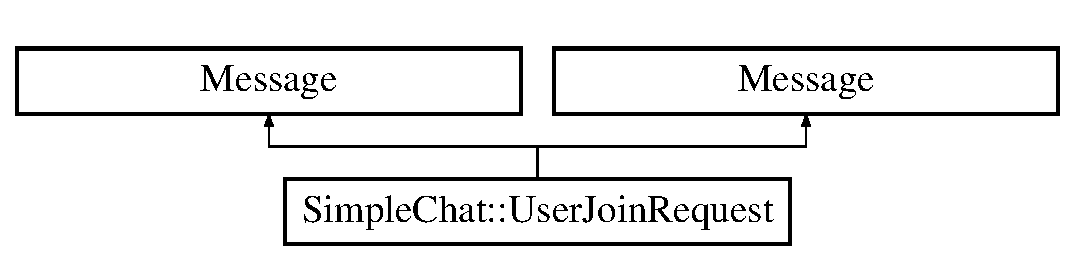
\includegraphics[height=2.000000cm]{classSimpleChat_1_1UserJoinRequest}
\end{center}
\end{figure}
\subsection*{Public Member Functions}
\begin{DoxyCompactItemize}
\item 
\hypertarget{classSimpleChat_1_1UserJoinRequest_a5c314549198119d803ebcae6f918e0df}{{\bfseries User\-Join\-Request} (const \hyperlink{classSimpleChat_1_1UserJoinRequest}{User\-Join\-Request} \&from)}\label{classSimpleChat_1_1UserJoinRequest_a5c314549198119d803ebcae6f918e0df}

\item 
\hypertarget{classSimpleChat_1_1UserJoinRequest_a94e16681aba97f45338f5273ef4844e1}{\hyperlink{classSimpleChat_1_1UserJoinRequest}{User\-Join\-Request} \& {\bfseries operator=} (const \hyperlink{classSimpleChat_1_1UserJoinRequest}{User\-Join\-Request} \&from)}\label{classSimpleChat_1_1UserJoinRequest_a94e16681aba97f45338f5273ef4844e1}

\item 
\hypertarget{classSimpleChat_1_1UserJoinRequest_a90b9270f5623668f8d121a5614f771d6}{const \\*
\-::google\-::protobuf\-::\-Unknown\-Field\-Set \& {\bfseries unknown\-\_\-fields} () const }\label{classSimpleChat_1_1UserJoinRequest_a90b9270f5623668f8d121a5614f771d6}

\item 
\hypertarget{classSimpleChat_1_1UserJoinRequest_a57ca214eb06071e26fef7d1bbb4b883d}{inline\-::google\-::protobuf\-::\-Unknown\-Field\-Set $\ast$ {\bfseries mutable\-\_\-unknown\-\_\-fields} ()}\label{classSimpleChat_1_1UserJoinRequest_a57ca214eb06071e26fef7d1bbb4b883d}

\item 
\hypertarget{classSimpleChat_1_1UserJoinRequest_a427d21d6091c09e761ebbba4a0d80393}{void {\bfseries Swap} (\hyperlink{classSimpleChat_1_1UserJoinRequest}{User\-Join\-Request} $\ast$other)}\label{classSimpleChat_1_1UserJoinRequest_a427d21d6091c09e761ebbba4a0d80393}

\item 
\hypertarget{classSimpleChat_1_1UserJoinRequest_a0150a989e981f3fd7251433b40864a51}{\hyperlink{classSimpleChat_1_1UserJoinRequest}{User\-Join\-Request} $\ast$ {\bfseries New} () const }\label{classSimpleChat_1_1UserJoinRequest_a0150a989e981f3fd7251433b40864a51}

\item 
\hypertarget{classSimpleChat_1_1UserJoinRequest_abd14064bf5bfe987d71cb7ed385eed16}{\hyperlink{classSimpleChat_1_1UserJoinRequest}{User\-Join\-Request} $\ast$ {\bfseries New} (\-::google\-::protobuf\-::\-Arena $\ast$arena) const }\label{classSimpleChat_1_1UserJoinRequest_abd14064bf5bfe987d71cb7ed385eed16}

\item 
\hypertarget{classSimpleChat_1_1UserJoinRequest_a9d76ddfb6ab5b38ddbe0ba0d1b2ebf0f}{void {\bfseries Copy\-From} (const \-::google\-::protobuf\-::\-Message \&from)}\label{classSimpleChat_1_1UserJoinRequest_a9d76ddfb6ab5b38ddbe0ba0d1b2ebf0f}

\item 
\hypertarget{classSimpleChat_1_1UserJoinRequest_a012014877340a6159c67ae1ce9fd56ba}{void {\bfseries Merge\-From} (const \-::google\-::protobuf\-::\-Message \&from)}\label{classSimpleChat_1_1UserJoinRequest_a012014877340a6159c67ae1ce9fd56ba}

\item 
\hypertarget{classSimpleChat_1_1UserJoinRequest_aed9ca7e9ba259a3b11d7112f1495199d}{void {\bfseries Copy\-From} (const \hyperlink{classSimpleChat_1_1UserJoinRequest}{User\-Join\-Request} \&from)}\label{classSimpleChat_1_1UserJoinRequest_aed9ca7e9ba259a3b11d7112f1495199d}

\item 
\hypertarget{classSimpleChat_1_1UserJoinRequest_a3ca2c2b4215c09d18b20e80763003e58}{void {\bfseries Merge\-From} (const \hyperlink{classSimpleChat_1_1UserJoinRequest}{User\-Join\-Request} \&from)}\label{classSimpleChat_1_1UserJoinRequest_a3ca2c2b4215c09d18b20e80763003e58}

\item 
\hypertarget{classSimpleChat_1_1UserJoinRequest_ad76d8b89c423d79df14823769d8ecb3d}{void {\bfseries Clear} ()}\label{classSimpleChat_1_1UserJoinRequest_ad76d8b89c423d79df14823769d8ecb3d}

\item 
\hypertarget{classSimpleChat_1_1UserJoinRequest_a568cfe228f12edb638d41b6abcb29882}{bool {\bfseries Is\-Initialized} () const }\label{classSimpleChat_1_1UserJoinRequest_a568cfe228f12edb638d41b6abcb29882}

\item 
\hypertarget{classSimpleChat_1_1UserJoinRequest_aa14f063d5d75fbec1b2b5f73a94d4bb7}{int {\bfseries Byte\-Size} () const }\label{classSimpleChat_1_1UserJoinRequest_aa14f063d5d75fbec1b2b5f73a94d4bb7}

\item 
\hypertarget{classSimpleChat_1_1UserJoinRequest_afbe311545f5d9162e81afb317c781092}{bool {\bfseries Merge\-Partial\-From\-Coded\-Stream} (\-::google\-::protobuf\-::io\-::\-Coded\-Input\-Stream $\ast$input)}\label{classSimpleChat_1_1UserJoinRequest_afbe311545f5d9162e81afb317c781092}

\item 
\hypertarget{classSimpleChat_1_1UserJoinRequest_a2f379a15168279f746bc4001b2c13e6c}{void {\bfseries Serialize\-With\-Cached\-Sizes} (\-::google\-::protobuf\-::io\-::\-Coded\-Output\-Stream $\ast$output) const }\label{classSimpleChat_1_1UserJoinRequest_a2f379a15168279f746bc4001b2c13e6c}

\item 
\hypertarget{classSimpleChat_1_1UserJoinRequest_a878da632abfb31d553d1b400b8f45a52}{\-::google\-::protobuf\-::uint8 $\ast$ {\bfseries Serialize\-With\-Cached\-Sizes\-To\-Array} (\-::google\-::protobuf\-::uint8 $\ast$output) const }\label{classSimpleChat_1_1UserJoinRequest_a878da632abfb31d553d1b400b8f45a52}

\item 
\hypertarget{classSimpleChat_1_1UserJoinRequest_a2b55ab3707e95fef478dbb684b170f1a}{int {\bfseries Get\-Cached\-Size} () const }\label{classSimpleChat_1_1UserJoinRequest_a2b55ab3707e95fef478dbb684b170f1a}

\item 
\hypertarget{classSimpleChat_1_1UserJoinRequest_a6d8bf1219cb5c587c2a4950895bfa0b5}{\-::google\-::protobuf\-::\-Metadata {\bfseries Get\-Metadata} () const }\label{classSimpleChat_1_1UserJoinRequest_a6d8bf1219cb5c587c2a4950895bfa0b5}

\item 
\hypertarget{classSimpleChat_1_1UserJoinRequest_a66d93d16639994f13157c9481451149b}{bool {\bfseries has\-\_\-name} () const }\label{classSimpleChat_1_1UserJoinRequest_a66d93d16639994f13157c9481451149b}

\item 
\hypertarget{classSimpleChat_1_1UserJoinRequest_a946ed8a97f22650e2880c26937f568b1}{void {\bfseries clear\-\_\-name} ()}\label{classSimpleChat_1_1UserJoinRequest_a946ed8a97f22650e2880c26937f568b1}

\item 
\hypertarget{classSimpleChat_1_1UserJoinRequest_a2982525dab4154b478bbec8e2e683bf7}{const \-::std\-::string \& {\bfseries name} () const }\label{classSimpleChat_1_1UserJoinRequest_a2982525dab4154b478bbec8e2e683bf7}

\item 
\hypertarget{classSimpleChat_1_1UserJoinRequest_a5eae1adb16b9eece46618eff667a4c90}{void {\bfseries set\-\_\-name} (const \-::std\-::string \&value)}\label{classSimpleChat_1_1UserJoinRequest_a5eae1adb16b9eece46618eff667a4c90}

\item 
\hypertarget{classSimpleChat_1_1UserJoinRequest_a4e28515fad8e2d4880ded647c8f85ca3}{void {\bfseries set\-\_\-name} (const char $\ast$value)}\label{classSimpleChat_1_1UserJoinRequest_a4e28515fad8e2d4880ded647c8f85ca3}

\item 
\hypertarget{classSimpleChat_1_1UserJoinRequest_a32515a7988d42d11d0892bfbf265a0f0}{void {\bfseries set\-\_\-name} (const char $\ast$value, size\-\_\-t size)}\label{classSimpleChat_1_1UserJoinRequest_a32515a7988d42d11d0892bfbf265a0f0}

\item 
\hypertarget{classSimpleChat_1_1UserJoinRequest_adc2f0a19ee7e0bfcbd0024c0217e2a34}{\-::std\-::string $\ast$ {\bfseries mutable\-\_\-name} ()}\label{classSimpleChat_1_1UserJoinRequest_adc2f0a19ee7e0bfcbd0024c0217e2a34}

\item 
\hypertarget{classSimpleChat_1_1UserJoinRequest_a42abc15d2a1e6a76b65d19d4d5cc8b29}{\-::std\-::string $\ast$ {\bfseries release\-\_\-name} ()}\label{classSimpleChat_1_1UserJoinRequest_a42abc15d2a1e6a76b65d19d4d5cc8b29}

\item 
\hypertarget{classSimpleChat_1_1UserJoinRequest_a6f0c2a29740247dd0b170ce1b91496e8}{void {\bfseries set\-\_\-allocated\-\_\-name} (\-::std\-::string $\ast$name)}\label{classSimpleChat_1_1UserJoinRequest_a6f0c2a29740247dd0b170ce1b91496e8}

\item 
\hypertarget{classSimpleChat_1_1UserJoinRequest_a5c314549198119d803ebcae6f918e0df}{{\bfseries User\-Join\-Request} (const \hyperlink{classSimpleChat_1_1UserJoinRequest}{User\-Join\-Request} \&from)}\label{classSimpleChat_1_1UserJoinRequest_a5c314549198119d803ebcae6f918e0df}

\item 
\hypertarget{classSimpleChat_1_1UserJoinRequest_a94e16681aba97f45338f5273ef4844e1}{\hyperlink{classSimpleChat_1_1UserJoinRequest}{User\-Join\-Request} \& {\bfseries operator=} (const \hyperlink{classSimpleChat_1_1UserJoinRequest}{User\-Join\-Request} \&from)}\label{classSimpleChat_1_1UserJoinRequest_a94e16681aba97f45338f5273ef4844e1}

\item 
\hypertarget{classSimpleChat_1_1UserJoinRequest_a90b9270f5623668f8d121a5614f771d6}{const \\*
\-::google\-::protobuf\-::\-Unknown\-Field\-Set \& {\bfseries unknown\-\_\-fields} () const }\label{classSimpleChat_1_1UserJoinRequest_a90b9270f5623668f8d121a5614f771d6}

\item 
\hypertarget{classSimpleChat_1_1UserJoinRequest_a57ca214eb06071e26fef7d1bbb4b883d}{inline\-::google\-::protobuf\-::\-Unknown\-Field\-Set $\ast$ {\bfseries mutable\-\_\-unknown\-\_\-fields} ()}\label{classSimpleChat_1_1UserJoinRequest_a57ca214eb06071e26fef7d1bbb4b883d}

\item 
\hypertarget{classSimpleChat_1_1UserJoinRequest_a427d21d6091c09e761ebbba4a0d80393}{void {\bfseries Swap} (\hyperlink{classSimpleChat_1_1UserJoinRequest}{User\-Join\-Request} $\ast$other)}\label{classSimpleChat_1_1UserJoinRequest_a427d21d6091c09e761ebbba4a0d80393}

\item 
\hypertarget{classSimpleChat_1_1UserJoinRequest_a0150a989e981f3fd7251433b40864a51}{\hyperlink{classSimpleChat_1_1UserJoinRequest}{User\-Join\-Request} $\ast$ {\bfseries New} () const }\label{classSimpleChat_1_1UserJoinRequest_a0150a989e981f3fd7251433b40864a51}

\item 
\hypertarget{classSimpleChat_1_1UserJoinRequest_abd14064bf5bfe987d71cb7ed385eed16}{\hyperlink{classSimpleChat_1_1UserJoinRequest}{User\-Join\-Request} $\ast$ {\bfseries New} (\-::google\-::protobuf\-::\-Arena $\ast$arena) const }\label{classSimpleChat_1_1UserJoinRequest_abd14064bf5bfe987d71cb7ed385eed16}

\item 
\hypertarget{classSimpleChat_1_1UserJoinRequest_a9d76ddfb6ab5b38ddbe0ba0d1b2ebf0f}{void {\bfseries Copy\-From} (const \-::google\-::protobuf\-::\-Message \&from)}\label{classSimpleChat_1_1UserJoinRequest_a9d76ddfb6ab5b38ddbe0ba0d1b2ebf0f}

\item 
\hypertarget{classSimpleChat_1_1UserJoinRequest_a012014877340a6159c67ae1ce9fd56ba}{void {\bfseries Merge\-From} (const \-::google\-::protobuf\-::\-Message \&from)}\label{classSimpleChat_1_1UserJoinRequest_a012014877340a6159c67ae1ce9fd56ba}

\item 
\hypertarget{classSimpleChat_1_1UserJoinRequest_aed9ca7e9ba259a3b11d7112f1495199d}{void {\bfseries Copy\-From} (const \hyperlink{classSimpleChat_1_1UserJoinRequest}{User\-Join\-Request} \&from)}\label{classSimpleChat_1_1UserJoinRequest_aed9ca7e9ba259a3b11d7112f1495199d}

\item 
\hypertarget{classSimpleChat_1_1UserJoinRequest_a3ca2c2b4215c09d18b20e80763003e58}{void {\bfseries Merge\-From} (const \hyperlink{classSimpleChat_1_1UserJoinRequest}{User\-Join\-Request} \&from)}\label{classSimpleChat_1_1UserJoinRequest_a3ca2c2b4215c09d18b20e80763003e58}

\item 
\hypertarget{classSimpleChat_1_1UserJoinRequest_ad76d8b89c423d79df14823769d8ecb3d}{void {\bfseries Clear} ()}\label{classSimpleChat_1_1UserJoinRequest_ad76d8b89c423d79df14823769d8ecb3d}

\item 
\hypertarget{classSimpleChat_1_1UserJoinRequest_a568cfe228f12edb638d41b6abcb29882}{bool {\bfseries Is\-Initialized} () const }\label{classSimpleChat_1_1UserJoinRequest_a568cfe228f12edb638d41b6abcb29882}

\item 
\hypertarget{classSimpleChat_1_1UserJoinRequest_aa14f063d5d75fbec1b2b5f73a94d4bb7}{int {\bfseries Byte\-Size} () const }\label{classSimpleChat_1_1UserJoinRequest_aa14f063d5d75fbec1b2b5f73a94d4bb7}

\item 
\hypertarget{classSimpleChat_1_1UserJoinRequest_afbe311545f5d9162e81afb317c781092}{bool {\bfseries Merge\-Partial\-From\-Coded\-Stream} (\-::google\-::protobuf\-::io\-::\-Coded\-Input\-Stream $\ast$input)}\label{classSimpleChat_1_1UserJoinRequest_afbe311545f5d9162e81afb317c781092}

\item 
\hypertarget{classSimpleChat_1_1UserJoinRequest_a2f379a15168279f746bc4001b2c13e6c}{void {\bfseries Serialize\-With\-Cached\-Sizes} (\-::google\-::protobuf\-::io\-::\-Coded\-Output\-Stream $\ast$output) const }\label{classSimpleChat_1_1UserJoinRequest_a2f379a15168279f746bc4001b2c13e6c}

\item 
\hypertarget{classSimpleChat_1_1UserJoinRequest_a878da632abfb31d553d1b400b8f45a52}{\-::google\-::protobuf\-::uint8 $\ast$ {\bfseries Serialize\-With\-Cached\-Sizes\-To\-Array} (\-::google\-::protobuf\-::uint8 $\ast$output) const }\label{classSimpleChat_1_1UserJoinRequest_a878da632abfb31d553d1b400b8f45a52}

\item 
\hypertarget{classSimpleChat_1_1UserJoinRequest_a2b55ab3707e95fef478dbb684b170f1a}{int {\bfseries Get\-Cached\-Size} () const }\label{classSimpleChat_1_1UserJoinRequest_a2b55ab3707e95fef478dbb684b170f1a}

\item 
\hypertarget{classSimpleChat_1_1UserJoinRequest_a6d8bf1219cb5c587c2a4950895bfa0b5}{\-::google\-::protobuf\-::\-Metadata {\bfseries Get\-Metadata} () const }\label{classSimpleChat_1_1UserJoinRequest_a6d8bf1219cb5c587c2a4950895bfa0b5}

\item 
\hypertarget{classSimpleChat_1_1UserJoinRequest_a66d93d16639994f13157c9481451149b}{bool {\bfseries has\-\_\-name} () const }\label{classSimpleChat_1_1UserJoinRequest_a66d93d16639994f13157c9481451149b}

\item 
\hypertarget{classSimpleChat_1_1UserJoinRequest_a946ed8a97f22650e2880c26937f568b1}{void {\bfseries clear\-\_\-name} ()}\label{classSimpleChat_1_1UserJoinRequest_a946ed8a97f22650e2880c26937f568b1}

\item 
\hypertarget{classSimpleChat_1_1UserJoinRequest_ab589c4f819f5bfbbb376d095211c6c30}{const \-::std\-::string \& {\bfseries name} () const }\label{classSimpleChat_1_1UserJoinRequest_ab589c4f819f5bfbbb376d095211c6c30}

\item 
\hypertarget{classSimpleChat_1_1UserJoinRequest_a5eae1adb16b9eece46618eff667a4c90}{void {\bfseries set\-\_\-name} (const \-::std\-::string \&value)}\label{classSimpleChat_1_1UserJoinRequest_a5eae1adb16b9eece46618eff667a4c90}

\item 
\hypertarget{classSimpleChat_1_1UserJoinRequest_a4e28515fad8e2d4880ded647c8f85ca3}{void {\bfseries set\-\_\-name} (const char $\ast$value)}\label{classSimpleChat_1_1UserJoinRequest_a4e28515fad8e2d4880ded647c8f85ca3}

\item 
\hypertarget{classSimpleChat_1_1UserJoinRequest_a32515a7988d42d11d0892bfbf265a0f0}{void {\bfseries set\-\_\-name} (const char $\ast$value, size\-\_\-t size)}\label{classSimpleChat_1_1UserJoinRequest_a32515a7988d42d11d0892bfbf265a0f0}

\item 
\hypertarget{classSimpleChat_1_1UserJoinRequest_a7ee5604db8a54484180f6dbf1804e226}{\-::std\-::string $\ast$ {\bfseries mutable\-\_\-name} ()}\label{classSimpleChat_1_1UserJoinRequest_a7ee5604db8a54484180f6dbf1804e226}

\item 
\hypertarget{classSimpleChat_1_1UserJoinRequest_a8a15455c39af181e71b437347daeed4d}{\-::std\-::string $\ast$ {\bfseries release\-\_\-name} ()}\label{classSimpleChat_1_1UserJoinRequest_a8a15455c39af181e71b437347daeed4d}

\item 
\hypertarget{classSimpleChat_1_1UserJoinRequest_a6f0c2a29740247dd0b170ce1b91496e8}{void {\bfseries set\-\_\-allocated\-\_\-name} (\-::std\-::string $\ast$name)}\label{classSimpleChat_1_1UserJoinRequest_a6f0c2a29740247dd0b170ce1b91496e8}

\end{DoxyCompactItemize}
\subsection*{Static Public Member Functions}
\begin{DoxyCompactItemize}
\item 
\hypertarget{classSimpleChat_1_1UserJoinRequest_a65cc9e081cd5f18c4e4c05949dd62108}{static const \\*
\-::google\-::protobuf\-::\-Descriptor $\ast$ {\bfseries descriptor} ()}\label{classSimpleChat_1_1UserJoinRequest_a65cc9e081cd5f18c4e4c05949dd62108}

\item 
\hypertarget{classSimpleChat_1_1UserJoinRequest_a7ec1f3e172f0e34068ca8772024ace92}{static const \hyperlink{classSimpleChat_1_1UserJoinRequest}{User\-Join\-Request} \& {\bfseries default\-\_\-instance} ()}\label{classSimpleChat_1_1UserJoinRequest_a7ec1f3e172f0e34068ca8772024ace92}

\item 
\hypertarget{classSimpleChat_1_1UserJoinRequest_a65cc9e081cd5f18c4e4c05949dd62108}{static const \\*
\-::google\-::protobuf\-::\-Descriptor $\ast$ {\bfseries descriptor} ()}\label{classSimpleChat_1_1UserJoinRequest_a65cc9e081cd5f18c4e4c05949dd62108}

\item 
\hypertarget{classSimpleChat_1_1UserJoinRequest_a7ec1f3e172f0e34068ca8772024ace92}{static const \hyperlink{classSimpleChat_1_1UserJoinRequest}{User\-Join\-Request} \& {\bfseries default\-\_\-instance} ()}\label{classSimpleChat_1_1UserJoinRequest_a7ec1f3e172f0e34068ca8772024ace92}

\end{DoxyCompactItemize}
\subsection*{Static Public Attributes}
\begin{DoxyCompactItemize}
\item 
\hypertarget{classSimpleChat_1_1UserJoinRequest_a033d146fbe3faeb8bb7f8583c372082e}{static const int {\bfseries k\-Name\-Field\-Number} = 1}\label{classSimpleChat_1_1UserJoinRequest_a033d146fbe3faeb8bb7f8583c372082e}

\end{DoxyCompactItemize}
\subsection*{Friends}
\begin{DoxyCompactItemize}
\item 
\hypertarget{classSimpleChat_1_1UserJoinRequest_a21c725e9955d4dda1abc79b117f57e76}{void {\bfseries protobuf\-\_\-\-Add\-Desc\-\_\-\-User\-\_\-2eproto} ()}\label{classSimpleChat_1_1UserJoinRequest_a21c725e9955d4dda1abc79b117f57e76}

\item 
\hypertarget{classSimpleChat_1_1UserJoinRequest_aadc83181f80ae5102c4449a54aef288e}{void {\bfseries protobuf\-\_\-\-Assign\-Desc\-\_\-\-User\-\_\-2eproto} ()}\label{classSimpleChat_1_1UserJoinRequest_aadc83181f80ae5102c4449a54aef288e}

\item 
\hypertarget{classSimpleChat_1_1UserJoinRequest_ac6d6bd3817a5978496745d793da7465f}{void {\bfseries protobuf\-\_\-\-Shutdown\-File\-\_\-\-User\-\_\-2eproto} ()}\label{classSimpleChat_1_1UserJoinRequest_ac6d6bd3817a5978496745d793da7465f}

\item 
\hypertarget{classSimpleChat_1_1UserJoinRequest_a21c725e9955d4dda1abc79b117f57e76}{void {\bfseries protobuf\-\_\-\-Add\-Desc\-\_\-\-User\-\_\-2eproto} ()}\label{classSimpleChat_1_1UserJoinRequest_a21c725e9955d4dda1abc79b117f57e76}

\item 
\hypertarget{classSimpleChat_1_1UserJoinRequest_aadc83181f80ae5102c4449a54aef288e}{void {\bfseries protobuf\-\_\-\-Assign\-Desc\-\_\-\-User\-\_\-2eproto} ()}\label{classSimpleChat_1_1UserJoinRequest_aadc83181f80ae5102c4449a54aef288e}

\item 
\hypertarget{classSimpleChat_1_1UserJoinRequest_ac6d6bd3817a5978496745d793da7465f}{void {\bfseries protobuf\-\_\-\-Shutdown\-File\-\_\-\-User\-\_\-2eproto} ()}\label{classSimpleChat_1_1UserJoinRequest_ac6d6bd3817a5978496745d793da7465f}

\end{DoxyCompactItemize}


The documentation for this class was generated from the following file\-:\begin{DoxyCompactItemize}
\item 
chatlib/proto/User.\-pb.\-h\end{DoxyCompactItemize}

\hypertarget{classSimpleChat_1_1UserJoinResponse}{\section{Simple\-Chat\-:\-:User\-Join\-Response Class Reference}
\label{classSimpleChat_1_1UserJoinResponse}\index{Simple\-Chat\-::\-User\-Join\-Response@{Simple\-Chat\-::\-User\-Join\-Response}}
}
Inheritance diagram for Simple\-Chat\-:\-:User\-Join\-Response\-:\begin{figure}[H]
\begin{center}
\leavevmode
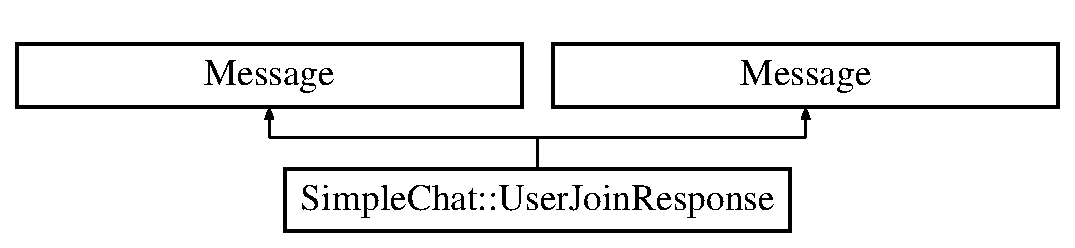
\includegraphics[height=2.000000cm]{classSimpleChat_1_1UserJoinResponse}
\end{center}
\end{figure}
\subsection*{Public Member Functions}
\begin{DoxyCompactItemize}
\item 
\hypertarget{classSimpleChat_1_1UserJoinResponse_a6ac5c504a53a80a0bd9b8135c83743e3}{{\bfseries User\-Join\-Response} (const \hyperlink{classSimpleChat_1_1UserJoinResponse}{User\-Join\-Response} \&from)}\label{classSimpleChat_1_1UserJoinResponse_a6ac5c504a53a80a0bd9b8135c83743e3}

\item 
\hypertarget{classSimpleChat_1_1UserJoinResponse_a7b819a45d55784fa256405d0a09ed471}{\hyperlink{classSimpleChat_1_1UserJoinResponse}{User\-Join\-Response} \& {\bfseries operator=} (const \hyperlink{classSimpleChat_1_1UserJoinResponse}{User\-Join\-Response} \&from)}\label{classSimpleChat_1_1UserJoinResponse_a7b819a45d55784fa256405d0a09ed471}

\item 
\hypertarget{classSimpleChat_1_1UserJoinResponse_a820b6d83a86ef347ce85fda4bdf322bd}{const \\*
\-::google\-::protobuf\-::\-Unknown\-Field\-Set \& {\bfseries unknown\-\_\-fields} () const }\label{classSimpleChat_1_1UserJoinResponse_a820b6d83a86ef347ce85fda4bdf322bd}

\item 
\hypertarget{classSimpleChat_1_1UserJoinResponse_a23f46f596005774a0873d889b00f97c5}{inline\-::google\-::protobuf\-::\-Unknown\-Field\-Set $\ast$ {\bfseries mutable\-\_\-unknown\-\_\-fields} ()}\label{classSimpleChat_1_1UserJoinResponse_a23f46f596005774a0873d889b00f97c5}

\item 
\hypertarget{classSimpleChat_1_1UserJoinResponse_ab94a5f942a0e4a200c8351b0cbd36020}{void {\bfseries Swap} (\hyperlink{classSimpleChat_1_1UserJoinResponse}{User\-Join\-Response} $\ast$other)}\label{classSimpleChat_1_1UserJoinResponse_ab94a5f942a0e4a200c8351b0cbd36020}

\item 
\hypertarget{classSimpleChat_1_1UserJoinResponse_aa2e8a1085ae0fcb0b672776215d696c2}{\hyperlink{classSimpleChat_1_1UserJoinResponse}{User\-Join\-Response} $\ast$ {\bfseries New} () const }\label{classSimpleChat_1_1UserJoinResponse_aa2e8a1085ae0fcb0b672776215d696c2}

\item 
\hypertarget{classSimpleChat_1_1UserJoinResponse_a96d7e67a29afa3393dc80fc3a61ff7e7}{\hyperlink{classSimpleChat_1_1UserJoinResponse}{User\-Join\-Response} $\ast$ {\bfseries New} (\-::google\-::protobuf\-::\-Arena $\ast$arena) const }\label{classSimpleChat_1_1UserJoinResponse_a96d7e67a29afa3393dc80fc3a61ff7e7}

\item 
\hypertarget{classSimpleChat_1_1UserJoinResponse_a294fddc7967202fa7900aab998eceb81}{void {\bfseries Copy\-From} (const \-::google\-::protobuf\-::\-Message \&from)}\label{classSimpleChat_1_1UserJoinResponse_a294fddc7967202fa7900aab998eceb81}

\item 
\hypertarget{classSimpleChat_1_1UserJoinResponse_ac83c9115a5c0cd55e0347fcc3ab4b2a3}{void {\bfseries Merge\-From} (const \-::google\-::protobuf\-::\-Message \&from)}\label{classSimpleChat_1_1UserJoinResponse_ac83c9115a5c0cd55e0347fcc3ab4b2a3}

\item 
\hypertarget{classSimpleChat_1_1UserJoinResponse_ac31245541435fbfd50017fdb4641fc92}{void {\bfseries Copy\-From} (const \hyperlink{classSimpleChat_1_1UserJoinResponse}{User\-Join\-Response} \&from)}\label{classSimpleChat_1_1UserJoinResponse_ac31245541435fbfd50017fdb4641fc92}

\item 
\hypertarget{classSimpleChat_1_1UserJoinResponse_a3a496db84f7ecbcb2daa5430dfae8849}{void {\bfseries Merge\-From} (const \hyperlink{classSimpleChat_1_1UserJoinResponse}{User\-Join\-Response} \&from)}\label{classSimpleChat_1_1UserJoinResponse_a3a496db84f7ecbcb2daa5430dfae8849}

\item 
\hypertarget{classSimpleChat_1_1UserJoinResponse_a578bc5bc15322ac410d9f8a0054009d3}{void {\bfseries Clear} ()}\label{classSimpleChat_1_1UserJoinResponse_a578bc5bc15322ac410d9f8a0054009d3}

\item 
\hypertarget{classSimpleChat_1_1UserJoinResponse_ac69e0bc7f005430285db03b4e1d94929}{bool {\bfseries Is\-Initialized} () const }\label{classSimpleChat_1_1UserJoinResponse_ac69e0bc7f005430285db03b4e1d94929}

\item 
\hypertarget{classSimpleChat_1_1UserJoinResponse_a7bc9bfc4416d0518e5f56ab724aa8402}{int {\bfseries Byte\-Size} () const }\label{classSimpleChat_1_1UserJoinResponse_a7bc9bfc4416d0518e5f56ab724aa8402}

\item 
\hypertarget{classSimpleChat_1_1UserJoinResponse_a7dcbfc3c35fb11afabea982e9e0ff766}{bool {\bfseries Merge\-Partial\-From\-Coded\-Stream} (\-::google\-::protobuf\-::io\-::\-Coded\-Input\-Stream $\ast$input)}\label{classSimpleChat_1_1UserJoinResponse_a7dcbfc3c35fb11afabea982e9e0ff766}

\item 
\hypertarget{classSimpleChat_1_1UserJoinResponse_a6efd7ade0c5cda0fd19d22333d613e66}{void {\bfseries Serialize\-With\-Cached\-Sizes} (\-::google\-::protobuf\-::io\-::\-Coded\-Output\-Stream $\ast$output) const }\label{classSimpleChat_1_1UserJoinResponse_a6efd7ade0c5cda0fd19d22333d613e66}

\item 
\hypertarget{classSimpleChat_1_1UserJoinResponse_a997ba4d2a92b010fd02f3cef8ca99f1d}{\-::google\-::protobuf\-::uint8 $\ast$ {\bfseries Serialize\-With\-Cached\-Sizes\-To\-Array} (\-::google\-::protobuf\-::uint8 $\ast$output) const }\label{classSimpleChat_1_1UserJoinResponse_a997ba4d2a92b010fd02f3cef8ca99f1d}

\item 
\hypertarget{classSimpleChat_1_1UserJoinResponse_a4c34493152ee3e2bd48ab9f778cd39e2}{int {\bfseries Get\-Cached\-Size} () const }\label{classSimpleChat_1_1UserJoinResponse_a4c34493152ee3e2bd48ab9f778cd39e2}

\item 
\hypertarget{classSimpleChat_1_1UserJoinResponse_a7cb0a528f8cade7293c587972d9e654d}{\-::google\-::protobuf\-::\-Metadata {\bfseries Get\-Metadata} () const }\label{classSimpleChat_1_1UserJoinResponse_a7cb0a528f8cade7293c587972d9e654d}

\item 
\hypertarget{classSimpleChat_1_1UserJoinResponse_a85eac5829d72c9b8bba643392109b20a}{bool {\bfseries has\-\_\-success} () const }\label{classSimpleChat_1_1UserJoinResponse_a85eac5829d72c9b8bba643392109b20a}

\item 
\hypertarget{classSimpleChat_1_1UserJoinResponse_a314674c3b695b99fa6205b529c12b4b1}{void {\bfseries clear\-\_\-success} ()}\label{classSimpleChat_1_1UserJoinResponse_a314674c3b695b99fa6205b529c12b4b1}

\item 
\hypertarget{classSimpleChat_1_1UserJoinResponse_ab1429a2461ce6875ee6fc9d28814b4ae}{bool {\bfseries success} () const }\label{classSimpleChat_1_1UserJoinResponse_ab1429a2461ce6875ee6fc9d28814b4ae}

\item 
\hypertarget{classSimpleChat_1_1UserJoinResponse_a91027dd2f3e2e44cfdee454cffc07f6c}{void {\bfseries set\-\_\-success} (bool value)}\label{classSimpleChat_1_1UserJoinResponse_a91027dd2f3e2e44cfdee454cffc07f6c}

\item 
\hypertarget{classSimpleChat_1_1UserJoinResponse_a0d883988b11d1698911f271e73f84e84}{bool {\bfseries has\-\_\-user} () const }\label{classSimpleChat_1_1UserJoinResponse_a0d883988b11d1698911f271e73f84e84}

\item 
\hypertarget{classSimpleChat_1_1UserJoinResponse_afa109451d5f37180a1b530e251bb9589}{void {\bfseries clear\-\_\-user} ()}\label{classSimpleChat_1_1UserJoinResponse_afa109451d5f37180a1b530e251bb9589}

\item 
\hypertarget{classSimpleChat_1_1UserJoinResponse_a640834b9c6f7f0025ac9ff0c5b8b0832}{const \-::\hyperlink{classSimpleChat_1_1User}{Simple\-Chat\-::\-User} \& {\bfseries user} () const }\label{classSimpleChat_1_1UserJoinResponse_a640834b9c6f7f0025ac9ff0c5b8b0832}

\item 
\hypertarget{classSimpleChat_1_1UserJoinResponse_ab18c1d6acde5b2981a56a51feccf7cfe}{\-::\hyperlink{classSimpleChat_1_1User}{Simple\-Chat\-::\-User} $\ast$ {\bfseries mutable\-\_\-user} ()}\label{classSimpleChat_1_1UserJoinResponse_ab18c1d6acde5b2981a56a51feccf7cfe}

\item 
\hypertarget{classSimpleChat_1_1UserJoinResponse_a952fbb6eed0e57bc70c13dbb5b17cd29}{\-::\hyperlink{classSimpleChat_1_1User}{Simple\-Chat\-::\-User} $\ast$ {\bfseries release\-\_\-user} ()}\label{classSimpleChat_1_1UserJoinResponse_a952fbb6eed0e57bc70c13dbb5b17cd29}

\item 
\hypertarget{classSimpleChat_1_1UserJoinResponse_a11a8cf027773c9d819e7c5cbdd02b9ed}{void {\bfseries set\-\_\-allocated\-\_\-user} (\-::\hyperlink{classSimpleChat_1_1User}{Simple\-Chat\-::\-User} $\ast$user)}\label{classSimpleChat_1_1UserJoinResponse_a11a8cf027773c9d819e7c5cbdd02b9ed}

\item 
\hypertarget{classSimpleChat_1_1UserJoinResponse_adbbb8921181991825ab0e5c1cf1b098f}{bool {\bfseries has\-\_\-motd} () const }\label{classSimpleChat_1_1UserJoinResponse_adbbb8921181991825ab0e5c1cf1b098f}

\item 
\hypertarget{classSimpleChat_1_1UserJoinResponse_a99f953920c1bb071ead4def21285df0a}{void {\bfseries clear\-\_\-motd} ()}\label{classSimpleChat_1_1UserJoinResponse_a99f953920c1bb071ead4def21285df0a}

\item 
\hypertarget{classSimpleChat_1_1UserJoinResponse_a1464667b9c359d30cd0c3584debef097}{const \-::std\-::string \& {\bfseries motd} () const }\label{classSimpleChat_1_1UserJoinResponse_a1464667b9c359d30cd0c3584debef097}

\item 
\hypertarget{classSimpleChat_1_1UserJoinResponse_ac47fd54dc7a6ef7a9f248b8eeda579c9}{void {\bfseries set\-\_\-motd} (const \-::std\-::string \&value)}\label{classSimpleChat_1_1UserJoinResponse_ac47fd54dc7a6ef7a9f248b8eeda579c9}

\item 
\hypertarget{classSimpleChat_1_1UserJoinResponse_aec17f78aa8ddf24bf4b9e09c16c08191}{void {\bfseries set\-\_\-motd} (const char $\ast$value)}\label{classSimpleChat_1_1UserJoinResponse_aec17f78aa8ddf24bf4b9e09c16c08191}

\item 
\hypertarget{classSimpleChat_1_1UserJoinResponse_a0094e222e6224bcc407fc525d4892677}{void {\bfseries set\-\_\-motd} (const char $\ast$value, size\-\_\-t size)}\label{classSimpleChat_1_1UserJoinResponse_a0094e222e6224bcc407fc525d4892677}

\item 
\hypertarget{classSimpleChat_1_1UserJoinResponse_a5a3332cf8f4dee17e15baa4b514ae438}{\-::std\-::string $\ast$ {\bfseries mutable\-\_\-motd} ()}\label{classSimpleChat_1_1UserJoinResponse_a5a3332cf8f4dee17e15baa4b514ae438}

\item 
\hypertarget{classSimpleChat_1_1UserJoinResponse_a634ed49c327c56e1da3f13410d4d8b60}{\-::std\-::string $\ast$ {\bfseries release\-\_\-motd} ()}\label{classSimpleChat_1_1UserJoinResponse_a634ed49c327c56e1da3f13410d4d8b60}

\item 
\hypertarget{classSimpleChat_1_1UserJoinResponse_a3b34f14eb142db56beadebfdcbccb9bc}{void {\bfseries set\-\_\-allocated\-\_\-motd} (\-::std\-::string $\ast$motd)}\label{classSimpleChat_1_1UserJoinResponse_a3b34f14eb142db56beadebfdcbccb9bc}

\item 
\hypertarget{classSimpleChat_1_1UserJoinResponse_ab8b2e9ca629c341a1114fecc41fe8b06}{bool {\bfseries has\-\_\-message} () const }\label{classSimpleChat_1_1UserJoinResponse_ab8b2e9ca629c341a1114fecc41fe8b06}

\item 
\hypertarget{classSimpleChat_1_1UserJoinResponse_a7520f7a1e1567db6eabecd90d3c549eb}{void {\bfseries clear\-\_\-message} ()}\label{classSimpleChat_1_1UserJoinResponse_a7520f7a1e1567db6eabecd90d3c549eb}

\item 
\hypertarget{classSimpleChat_1_1UserJoinResponse_a9d014b8ad8030da0a407d2b85fde95c1}{const \-::std\-::string \& {\bfseries message} () const }\label{classSimpleChat_1_1UserJoinResponse_a9d014b8ad8030da0a407d2b85fde95c1}

\item 
\hypertarget{classSimpleChat_1_1UserJoinResponse_ae284b05b50010230fac061f9a63555cf}{void {\bfseries set\-\_\-message} (const \-::std\-::string \&value)}\label{classSimpleChat_1_1UserJoinResponse_ae284b05b50010230fac061f9a63555cf}

\item 
\hypertarget{classSimpleChat_1_1UserJoinResponse_a89be458afc1d17022948e78ce5012d01}{void {\bfseries set\-\_\-message} (const char $\ast$value)}\label{classSimpleChat_1_1UserJoinResponse_a89be458afc1d17022948e78ce5012d01}

\item 
\hypertarget{classSimpleChat_1_1UserJoinResponse_a63c1f7f88f7f2cbea3ce7760f4304a9f}{void {\bfseries set\-\_\-message} (const char $\ast$value, size\-\_\-t size)}\label{classSimpleChat_1_1UserJoinResponse_a63c1f7f88f7f2cbea3ce7760f4304a9f}

\item 
\hypertarget{classSimpleChat_1_1UserJoinResponse_af83bf2f000e4eb8d94fdb7dcfd5294c1}{\-::std\-::string $\ast$ {\bfseries mutable\-\_\-message} ()}\label{classSimpleChat_1_1UserJoinResponse_af83bf2f000e4eb8d94fdb7dcfd5294c1}

\item 
\hypertarget{classSimpleChat_1_1UserJoinResponse_a6e63ebf7f109e35143f972e400353401}{\-::std\-::string $\ast$ {\bfseries release\-\_\-message} ()}\label{classSimpleChat_1_1UserJoinResponse_a6e63ebf7f109e35143f972e400353401}

\item 
\hypertarget{classSimpleChat_1_1UserJoinResponse_af8e62cfb486c721d18f77e48ab00d143}{void {\bfseries set\-\_\-allocated\-\_\-message} (\-::std\-::string $\ast$message)}\label{classSimpleChat_1_1UserJoinResponse_af8e62cfb486c721d18f77e48ab00d143}

\item 
\hypertarget{classSimpleChat_1_1UserJoinResponse_a6ac5c504a53a80a0bd9b8135c83743e3}{{\bfseries User\-Join\-Response} (const \hyperlink{classSimpleChat_1_1UserJoinResponse}{User\-Join\-Response} \&from)}\label{classSimpleChat_1_1UserJoinResponse_a6ac5c504a53a80a0bd9b8135c83743e3}

\item 
\hypertarget{classSimpleChat_1_1UserJoinResponse_a7b819a45d55784fa256405d0a09ed471}{\hyperlink{classSimpleChat_1_1UserJoinResponse}{User\-Join\-Response} \& {\bfseries operator=} (const \hyperlink{classSimpleChat_1_1UserJoinResponse}{User\-Join\-Response} \&from)}\label{classSimpleChat_1_1UserJoinResponse_a7b819a45d55784fa256405d0a09ed471}

\item 
\hypertarget{classSimpleChat_1_1UserJoinResponse_a820b6d83a86ef347ce85fda4bdf322bd}{const \\*
\-::google\-::protobuf\-::\-Unknown\-Field\-Set \& {\bfseries unknown\-\_\-fields} () const }\label{classSimpleChat_1_1UserJoinResponse_a820b6d83a86ef347ce85fda4bdf322bd}

\item 
\hypertarget{classSimpleChat_1_1UserJoinResponse_a23f46f596005774a0873d889b00f97c5}{inline\-::google\-::protobuf\-::\-Unknown\-Field\-Set $\ast$ {\bfseries mutable\-\_\-unknown\-\_\-fields} ()}\label{classSimpleChat_1_1UserJoinResponse_a23f46f596005774a0873d889b00f97c5}

\item 
\hypertarget{classSimpleChat_1_1UserJoinResponse_ab94a5f942a0e4a200c8351b0cbd36020}{void {\bfseries Swap} (\hyperlink{classSimpleChat_1_1UserJoinResponse}{User\-Join\-Response} $\ast$other)}\label{classSimpleChat_1_1UserJoinResponse_ab94a5f942a0e4a200c8351b0cbd36020}

\item 
\hypertarget{classSimpleChat_1_1UserJoinResponse_aa2e8a1085ae0fcb0b672776215d696c2}{\hyperlink{classSimpleChat_1_1UserJoinResponse}{User\-Join\-Response} $\ast$ {\bfseries New} () const }\label{classSimpleChat_1_1UserJoinResponse_aa2e8a1085ae0fcb0b672776215d696c2}

\item 
\hypertarget{classSimpleChat_1_1UserJoinResponse_a96d7e67a29afa3393dc80fc3a61ff7e7}{\hyperlink{classSimpleChat_1_1UserJoinResponse}{User\-Join\-Response} $\ast$ {\bfseries New} (\-::google\-::protobuf\-::\-Arena $\ast$arena) const }\label{classSimpleChat_1_1UserJoinResponse_a96d7e67a29afa3393dc80fc3a61ff7e7}

\item 
\hypertarget{classSimpleChat_1_1UserJoinResponse_a294fddc7967202fa7900aab998eceb81}{void {\bfseries Copy\-From} (const \-::google\-::protobuf\-::\-Message \&from)}\label{classSimpleChat_1_1UserJoinResponse_a294fddc7967202fa7900aab998eceb81}

\item 
\hypertarget{classSimpleChat_1_1UserJoinResponse_ac83c9115a5c0cd55e0347fcc3ab4b2a3}{void {\bfseries Merge\-From} (const \-::google\-::protobuf\-::\-Message \&from)}\label{classSimpleChat_1_1UserJoinResponse_ac83c9115a5c0cd55e0347fcc3ab4b2a3}

\item 
\hypertarget{classSimpleChat_1_1UserJoinResponse_ac31245541435fbfd50017fdb4641fc92}{void {\bfseries Copy\-From} (const \hyperlink{classSimpleChat_1_1UserJoinResponse}{User\-Join\-Response} \&from)}\label{classSimpleChat_1_1UserJoinResponse_ac31245541435fbfd50017fdb4641fc92}

\item 
\hypertarget{classSimpleChat_1_1UserJoinResponse_a3a496db84f7ecbcb2daa5430dfae8849}{void {\bfseries Merge\-From} (const \hyperlink{classSimpleChat_1_1UserJoinResponse}{User\-Join\-Response} \&from)}\label{classSimpleChat_1_1UserJoinResponse_a3a496db84f7ecbcb2daa5430dfae8849}

\item 
\hypertarget{classSimpleChat_1_1UserJoinResponse_a578bc5bc15322ac410d9f8a0054009d3}{void {\bfseries Clear} ()}\label{classSimpleChat_1_1UserJoinResponse_a578bc5bc15322ac410d9f8a0054009d3}

\item 
\hypertarget{classSimpleChat_1_1UserJoinResponse_ac69e0bc7f005430285db03b4e1d94929}{bool {\bfseries Is\-Initialized} () const }\label{classSimpleChat_1_1UserJoinResponse_ac69e0bc7f005430285db03b4e1d94929}

\item 
\hypertarget{classSimpleChat_1_1UserJoinResponse_a7bc9bfc4416d0518e5f56ab724aa8402}{int {\bfseries Byte\-Size} () const }\label{classSimpleChat_1_1UserJoinResponse_a7bc9bfc4416d0518e5f56ab724aa8402}

\item 
\hypertarget{classSimpleChat_1_1UserJoinResponse_a7dcbfc3c35fb11afabea982e9e0ff766}{bool {\bfseries Merge\-Partial\-From\-Coded\-Stream} (\-::google\-::protobuf\-::io\-::\-Coded\-Input\-Stream $\ast$input)}\label{classSimpleChat_1_1UserJoinResponse_a7dcbfc3c35fb11afabea982e9e0ff766}

\item 
\hypertarget{classSimpleChat_1_1UserJoinResponse_a6efd7ade0c5cda0fd19d22333d613e66}{void {\bfseries Serialize\-With\-Cached\-Sizes} (\-::google\-::protobuf\-::io\-::\-Coded\-Output\-Stream $\ast$output) const }\label{classSimpleChat_1_1UserJoinResponse_a6efd7ade0c5cda0fd19d22333d613e66}

\item 
\hypertarget{classSimpleChat_1_1UserJoinResponse_a997ba4d2a92b010fd02f3cef8ca99f1d}{\-::google\-::protobuf\-::uint8 $\ast$ {\bfseries Serialize\-With\-Cached\-Sizes\-To\-Array} (\-::google\-::protobuf\-::uint8 $\ast$output) const }\label{classSimpleChat_1_1UserJoinResponse_a997ba4d2a92b010fd02f3cef8ca99f1d}

\item 
\hypertarget{classSimpleChat_1_1UserJoinResponse_a4c34493152ee3e2bd48ab9f778cd39e2}{int {\bfseries Get\-Cached\-Size} () const }\label{classSimpleChat_1_1UserJoinResponse_a4c34493152ee3e2bd48ab9f778cd39e2}

\item 
\hypertarget{classSimpleChat_1_1UserJoinResponse_a7cb0a528f8cade7293c587972d9e654d}{\-::google\-::protobuf\-::\-Metadata {\bfseries Get\-Metadata} () const }\label{classSimpleChat_1_1UserJoinResponse_a7cb0a528f8cade7293c587972d9e654d}

\item 
\hypertarget{classSimpleChat_1_1UserJoinResponse_a85eac5829d72c9b8bba643392109b20a}{bool {\bfseries has\-\_\-success} () const }\label{classSimpleChat_1_1UserJoinResponse_a85eac5829d72c9b8bba643392109b20a}

\item 
\hypertarget{classSimpleChat_1_1UserJoinResponse_a314674c3b695b99fa6205b529c12b4b1}{void {\bfseries clear\-\_\-success} ()}\label{classSimpleChat_1_1UserJoinResponse_a314674c3b695b99fa6205b529c12b4b1}

\item 
\hypertarget{classSimpleChat_1_1UserJoinResponse_ab1429a2461ce6875ee6fc9d28814b4ae}{bool {\bfseries success} () const }\label{classSimpleChat_1_1UserJoinResponse_ab1429a2461ce6875ee6fc9d28814b4ae}

\item 
\hypertarget{classSimpleChat_1_1UserJoinResponse_a91027dd2f3e2e44cfdee454cffc07f6c}{void {\bfseries set\-\_\-success} (bool value)}\label{classSimpleChat_1_1UserJoinResponse_a91027dd2f3e2e44cfdee454cffc07f6c}

\item 
\hypertarget{classSimpleChat_1_1UserJoinResponse_a0d883988b11d1698911f271e73f84e84}{bool {\bfseries has\-\_\-user} () const }\label{classSimpleChat_1_1UserJoinResponse_a0d883988b11d1698911f271e73f84e84}

\item 
\hypertarget{classSimpleChat_1_1UserJoinResponse_afa109451d5f37180a1b530e251bb9589}{void {\bfseries clear\-\_\-user} ()}\label{classSimpleChat_1_1UserJoinResponse_afa109451d5f37180a1b530e251bb9589}

\item 
\hypertarget{classSimpleChat_1_1UserJoinResponse_a32ef80475c39ae99ed9b886f9bc1753e}{const \-::\hyperlink{classSimpleChat_1_1User}{Simple\-Chat\-::\-User} \& {\bfseries user} () const }\label{classSimpleChat_1_1UserJoinResponse_a32ef80475c39ae99ed9b886f9bc1753e}

\item 
\hypertarget{classSimpleChat_1_1UserJoinResponse_af47d495e664c660a8885cd943072aef8}{\-::\hyperlink{classSimpleChat_1_1User}{Simple\-Chat\-::\-User} $\ast$ {\bfseries mutable\-\_\-user} ()}\label{classSimpleChat_1_1UserJoinResponse_af47d495e664c660a8885cd943072aef8}

\item 
\hypertarget{classSimpleChat_1_1UserJoinResponse_a711c73e3d9315a7790a45a2072c7bd7f}{\-::\hyperlink{classSimpleChat_1_1User}{Simple\-Chat\-::\-User} $\ast$ {\bfseries release\-\_\-user} ()}\label{classSimpleChat_1_1UserJoinResponse_a711c73e3d9315a7790a45a2072c7bd7f}

\item 
\hypertarget{classSimpleChat_1_1UserJoinResponse_a11a8cf027773c9d819e7c5cbdd02b9ed}{void {\bfseries set\-\_\-allocated\-\_\-user} (\-::\hyperlink{classSimpleChat_1_1User}{Simple\-Chat\-::\-User} $\ast$user)}\label{classSimpleChat_1_1UserJoinResponse_a11a8cf027773c9d819e7c5cbdd02b9ed}

\item 
\hypertarget{classSimpleChat_1_1UserJoinResponse_adbbb8921181991825ab0e5c1cf1b098f}{bool {\bfseries has\-\_\-motd} () const }\label{classSimpleChat_1_1UserJoinResponse_adbbb8921181991825ab0e5c1cf1b098f}

\item 
\hypertarget{classSimpleChat_1_1UserJoinResponse_a99f953920c1bb071ead4def21285df0a}{void {\bfseries clear\-\_\-motd} ()}\label{classSimpleChat_1_1UserJoinResponse_a99f953920c1bb071ead4def21285df0a}

\item 
\hypertarget{classSimpleChat_1_1UserJoinResponse_add2f562513eb23156c5c83686d07b98c}{const \-::std\-::string \& {\bfseries motd} () const }\label{classSimpleChat_1_1UserJoinResponse_add2f562513eb23156c5c83686d07b98c}

\item 
\hypertarget{classSimpleChat_1_1UserJoinResponse_ac47fd54dc7a6ef7a9f248b8eeda579c9}{void {\bfseries set\-\_\-motd} (const \-::std\-::string \&value)}\label{classSimpleChat_1_1UserJoinResponse_ac47fd54dc7a6ef7a9f248b8eeda579c9}

\item 
\hypertarget{classSimpleChat_1_1UserJoinResponse_aec17f78aa8ddf24bf4b9e09c16c08191}{void {\bfseries set\-\_\-motd} (const char $\ast$value)}\label{classSimpleChat_1_1UserJoinResponse_aec17f78aa8ddf24bf4b9e09c16c08191}

\item 
\hypertarget{classSimpleChat_1_1UserJoinResponse_a0094e222e6224bcc407fc525d4892677}{void {\bfseries set\-\_\-motd} (const char $\ast$value, size\-\_\-t size)}\label{classSimpleChat_1_1UserJoinResponse_a0094e222e6224bcc407fc525d4892677}

\item 
\hypertarget{classSimpleChat_1_1UserJoinResponse_a2637713e2d9a9ce8e5a64f5b73f546e7}{\-::std\-::string $\ast$ {\bfseries mutable\-\_\-motd} ()}\label{classSimpleChat_1_1UserJoinResponse_a2637713e2d9a9ce8e5a64f5b73f546e7}

\item 
\hypertarget{classSimpleChat_1_1UserJoinResponse_a77867d5c002b00d8102d3bd780e488cd}{\-::std\-::string $\ast$ {\bfseries release\-\_\-motd} ()}\label{classSimpleChat_1_1UserJoinResponse_a77867d5c002b00d8102d3bd780e488cd}

\item 
\hypertarget{classSimpleChat_1_1UserJoinResponse_a3b34f14eb142db56beadebfdcbccb9bc}{void {\bfseries set\-\_\-allocated\-\_\-motd} (\-::std\-::string $\ast$motd)}\label{classSimpleChat_1_1UserJoinResponse_a3b34f14eb142db56beadebfdcbccb9bc}

\item 
\hypertarget{classSimpleChat_1_1UserJoinResponse_ab8b2e9ca629c341a1114fecc41fe8b06}{bool {\bfseries has\-\_\-message} () const }\label{classSimpleChat_1_1UserJoinResponse_ab8b2e9ca629c341a1114fecc41fe8b06}

\item 
\hypertarget{classSimpleChat_1_1UserJoinResponse_a7520f7a1e1567db6eabecd90d3c549eb}{void {\bfseries clear\-\_\-message} ()}\label{classSimpleChat_1_1UserJoinResponse_a7520f7a1e1567db6eabecd90d3c549eb}

\item 
\hypertarget{classSimpleChat_1_1UserJoinResponse_a58049d0c1a8973844d16ce57244de794}{const \-::std\-::string \& {\bfseries message} () const }\label{classSimpleChat_1_1UserJoinResponse_a58049d0c1a8973844d16ce57244de794}

\item 
\hypertarget{classSimpleChat_1_1UserJoinResponse_ae284b05b50010230fac061f9a63555cf}{void {\bfseries set\-\_\-message} (const \-::std\-::string \&value)}\label{classSimpleChat_1_1UserJoinResponse_ae284b05b50010230fac061f9a63555cf}

\item 
\hypertarget{classSimpleChat_1_1UserJoinResponse_a89be458afc1d17022948e78ce5012d01}{void {\bfseries set\-\_\-message} (const char $\ast$value)}\label{classSimpleChat_1_1UserJoinResponse_a89be458afc1d17022948e78ce5012d01}

\item 
\hypertarget{classSimpleChat_1_1UserJoinResponse_a63c1f7f88f7f2cbea3ce7760f4304a9f}{void {\bfseries set\-\_\-message} (const char $\ast$value, size\-\_\-t size)}\label{classSimpleChat_1_1UserJoinResponse_a63c1f7f88f7f2cbea3ce7760f4304a9f}

\item 
\hypertarget{classSimpleChat_1_1UserJoinResponse_af5841bb494f4a00ca6211b8ab21ec186}{\-::std\-::string $\ast$ {\bfseries mutable\-\_\-message} ()}\label{classSimpleChat_1_1UserJoinResponse_af5841bb494f4a00ca6211b8ab21ec186}

\item 
\hypertarget{classSimpleChat_1_1UserJoinResponse_afb3a3c489f2f7f1ec8af2d4da3486a99}{\-::std\-::string $\ast$ {\bfseries release\-\_\-message} ()}\label{classSimpleChat_1_1UserJoinResponse_afb3a3c489f2f7f1ec8af2d4da3486a99}

\item 
\hypertarget{classSimpleChat_1_1UserJoinResponse_af8e62cfb486c721d18f77e48ab00d143}{void {\bfseries set\-\_\-allocated\-\_\-message} (\-::std\-::string $\ast$message)}\label{classSimpleChat_1_1UserJoinResponse_af8e62cfb486c721d18f77e48ab00d143}

\end{DoxyCompactItemize}
\subsection*{Static Public Member Functions}
\begin{DoxyCompactItemize}
\item 
\hypertarget{classSimpleChat_1_1UserJoinResponse_a0edb2769e2ef85355cd1d6724bd3b0fd}{static const \\*
\-::google\-::protobuf\-::\-Descriptor $\ast$ {\bfseries descriptor} ()}\label{classSimpleChat_1_1UserJoinResponse_a0edb2769e2ef85355cd1d6724bd3b0fd}

\item 
\hypertarget{classSimpleChat_1_1UserJoinResponse_a4c18ad7705f6ad5eb6b6de0258130100}{static const \hyperlink{classSimpleChat_1_1UserJoinResponse}{User\-Join\-Response} \& {\bfseries default\-\_\-instance} ()}\label{classSimpleChat_1_1UserJoinResponse_a4c18ad7705f6ad5eb6b6de0258130100}

\item 
\hypertarget{classSimpleChat_1_1UserJoinResponse_a0edb2769e2ef85355cd1d6724bd3b0fd}{static const \\*
\-::google\-::protobuf\-::\-Descriptor $\ast$ {\bfseries descriptor} ()}\label{classSimpleChat_1_1UserJoinResponse_a0edb2769e2ef85355cd1d6724bd3b0fd}

\item 
\hypertarget{classSimpleChat_1_1UserJoinResponse_a4c18ad7705f6ad5eb6b6de0258130100}{static const \hyperlink{classSimpleChat_1_1UserJoinResponse}{User\-Join\-Response} \& {\bfseries default\-\_\-instance} ()}\label{classSimpleChat_1_1UserJoinResponse_a4c18ad7705f6ad5eb6b6de0258130100}

\end{DoxyCompactItemize}
\subsection*{Static Public Attributes}
\begin{DoxyCompactItemize}
\item 
\hypertarget{classSimpleChat_1_1UserJoinResponse_af247b57838290c1586ec1dd83e562416}{static const int {\bfseries k\-Success\-Field\-Number} = 1}\label{classSimpleChat_1_1UserJoinResponse_af247b57838290c1586ec1dd83e562416}

\item 
\hypertarget{classSimpleChat_1_1UserJoinResponse_af499f2a7842a6be1f266407689905686}{static const int {\bfseries k\-User\-Field\-Number} = 2}\label{classSimpleChat_1_1UserJoinResponse_af499f2a7842a6be1f266407689905686}

\item 
\hypertarget{classSimpleChat_1_1UserJoinResponse_ad26f1f7fd5859e1fe5429440d3607a64}{static const int {\bfseries k\-Motd\-Field\-Number} = 3}\label{classSimpleChat_1_1UserJoinResponse_ad26f1f7fd5859e1fe5429440d3607a64}

\item 
\hypertarget{classSimpleChat_1_1UserJoinResponse_a27bbc3323ad55f74c9377d9802669126}{static const int {\bfseries k\-Message\-Field\-Number} = 4}\label{classSimpleChat_1_1UserJoinResponse_a27bbc3323ad55f74c9377d9802669126}

\end{DoxyCompactItemize}
\subsection*{Friends}
\begin{DoxyCompactItemize}
\item 
\hypertarget{classSimpleChat_1_1UserJoinResponse_a21c725e9955d4dda1abc79b117f57e76}{void {\bfseries protobuf\-\_\-\-Add\-Desc\-\_\-\-User\-\_\-2eproto} ()}\label{classSimpleChat_1_1UserJoinResponse_a21c725e9955d4dda1abc79b117f57e76}

\item 
\hypertarget{classSimpleChat_1_1UserJoinResponse_aadc83181f80ae5102c4449a54aef288e}{void {\bfseries protobuf\-\_\-\-Assign\-Desc\-\_\-\-User\-\_\-2eproto} ()}\label{classSimpleChat_1_1UserJoinResponse_aadc83181f80ae5102c4449a54aef288e}

\item 
\hypertarget{classSimpleChat_1_1UserJoinResponse_ac6d6bd3817a5978496745d793da7465f}{void {\bfseries protobuf\-\_\-\-Shutdown\-File\-\_\-\-User\-\_\-2eproto} ()}\label{classSimpleChat_1_1UserJoinResponse_ac6d6bd3817a5978496745d793da7465f}

\item 
\hypertarget{classSimpleChat_1_1UserJoinResponse_a21c725e9955d4dda1abc79b117f57e76}{void {\bfseries protobuf\-\_\-\-Add\-Desc\-\_\-\-User\-\_\-2eproto} ()}\label{classSimpleChat_1_1UserJoinResponse_a21c725e9955d4dda1abc79b117f57e76}

\item 
\hypertarget{classSimpleChat_1_1UserJoinResponse_aadc83181f80ae5102c4449a54aef288e}{void {\bfseries protobuf\-\_\-\-Assign\-Desc\-\_\-\-User\-\_\-2eproto} ()}\label{classSimpleChat_1_1UserJoinResponse_aadc83181f80ae5102c4449a54aef288e}

\item 
\hypertarget{classSimpleChat_1_1UserJoinResponse_ac6d6bd3817a5978496745d793da7465f}{void {\bfseries protobuf\-\_\-\-Shutdown\-File\-\_\-\-User\-\_\-2eproto} ()}\label{classSimpleChat_1_1UserJoinResponse_ac6d6bd3817a5978496745d793da7465f}

\end{DoxyCompactItemize}


The documentation for this class was generated from the following file\-:\begin{DoxyCompactItemize}
\item 
chatlib/proto/User.\-pb.\-h\end{DoxyCompactItemize}

\hypertarget{classSimpleChat_1_1UserListRequest}{\section{Simple\-Chat\-:\-:User\-List\-Request Class Reference}
\label{classSimpleChat_1_1UserListRequest}\index{Simple\-Chat\-::\-User\-List\-Request@{Simple\-Chat\-::\-User\-List\-Request}}
}
Inheritance diagram for Simple\-Chat\-:\-:User\-List\-Request\-:\begin{figure}[H]
\begin{center}
\leavevmode
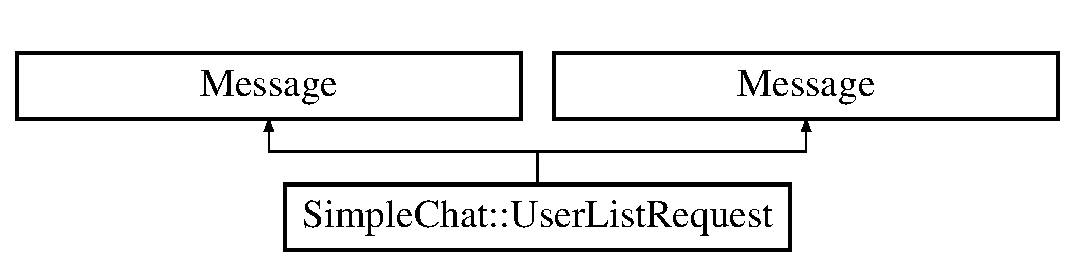
\includegraphics[height=2.000000cm]{classSimpleChat_1_1UserListRequest}
\end{center}
\end{figure}
\subsection*{Public Member Functions}
\begin{DoxyCompactItemize}
\item 
\hypertarget{classSimpleChat_1_1UserListRequest_adf87a872a0904fb5a015a27dc9ed615b}{{\bfseries User\-List\-Request} (const \hyperlink{classSimpleChat_1_1UserListRequest}{User\-List\-Request} \&from)}\label{classSimpleChat_1_1UserListRequest_adf87a872a0904fb5a015a27dc9ed615b}

\item 
\hypertarget{classSimpleChat_1_1UserListRequest_a44923332cb0344abc96ef3adecd31a64}{\hyperlink{classSimpleChat_1_1UserListRequest}{User\-List\-Request} \& {\bfseries operator=} (const \hyperlink{classSimpleChat_1_1UserListRequest}{User\-List\-Request} \&from)}\label{classSimpleChat_1_1UserListRequest_a44923332cb0344abc96ef3adecd31a64}

\item 
\hypertarget{classSimpleChat_1_1UserListRequest_a3e0db8f83f36267008abb4e79b3df138}{const \\*
\-::google\-::protobuf\-::\-Unknown\-Field\-Set \& {\bfseries unknown\-\_\-fields} () const }\label{classSimpleChat_1_1UserListRequest_a3e0db8f83f36267008abb4e79b3df138}

\item 
\hypertarget{classSimpleChat_1_1UserListRequest_aa1fc777d8e850616b3d3ebc023bb5b04}{inline\-::google\-::protobuf\-::\-Unknown\-Field\-Set $\ast$ {\bfseries mutable\-\_\-unknown\-\_\-fields} ()}\label{classSimpleChat_1_1UserListRequest_aa1fc777d8e850616b3d3ebc023bb5b04}

\item 
\hypertarget{classSimpleChat_1_1UserListRequest_ae301e4d1c6d099a73f2b6f9b938234a4}{void {\bfseries Swap} (\hyperlink{classSimpleChat_1_1UserListRequest}{User\-List\-Request} $\ast$other)}\label{classSimpleChat_1_1UserListRequest_ae301e4d1c6d099a73f2b6f9b938234a4}

\item 
\hypertarget{classSimpleChat_1_1UserListRequest_a7a1c940050451424a13ced56a5a25528}{\hyperlink{classSimpleChat_1_1UserListRequest}{User\-List\-Request} $\ast$ {\bfseries New} () const }\label{classSimpleChat_1_1UserListRequest_a7a1c940050451424a13ced56a5a25528}

\item 
\hypertarget{classSimpleChat_1_1UserListRequest_a68b46b687074a254fc37acf6049527b1}{\hyperlink{classSimpleChat_1_1UserListRequest}{User\-List\-Request} $\ast$ {\bfseries New} (\-::google\-::protobuf\-::\-Arena $\ast$arena) const }\label{classSimpleChat_1_1UserListRequest_a68b46b687074a254fc37acf6049527b1}

\item 
\hypertarget{classSimpleChat_1_1UserListRequest_a0b9f4fd9c2b1681d503e73ab4520b338}{void {\bfseries Copy\-From} (const \-::google\-::protobuf\-::\-Message \&from)}\label{classSimpleChat_1_1UserListRequest_a0b9f4fd9c2b1681d503e73ab4520b338}

\item 
\hypertarget{classSimpleChat_1_1UserListRequest_a0b16ebd3e4c4d309c36601e874ce096b}{void {\bfseries Merge\-From} (const \-::google\-::protobuf\-::\-Message \&from)}\label{classSimpleChat_1_1UserListRequest_a0b16ebd3e4c4d309c36601e874ce096b}

\item 
\hypertarget{classSimpleChat_1_1UserListRequest_ab7727ed54ac9484bb37c2ed6183daf92}{void {\bfseries Copy\-From} (const \hyperlink{classSimpleChat_1_1UserListRequest}{User\-List\-Request} \&from)}\label{classSimpleChat_1_1UserListRequest_ab7727ed54ac9484bb37c2ed6183daf92}

\item 
\hypertarget{classSimpleChat_1_1UserListRequest_aff4c8bebd90862effd88416b5403e54d}{void {\bfseries Merge\-From} (const \hyperlink{classSimpleChat_1_1UserListRequest}{User\-List\-Request} \&from)}\label{classSimpleChat_1_1UserListRequest_aff4c8bebd90862effd88416b5403e54d}

\item 
\hypertarget{classSimpleChat_1_1UserListRequest_af48c6b644eb5e6a37125a1a87288ef95}{void {\bfseries Clear} ()}\label{classSimpleChat_1_1UserListRequest_af48c6b644eb5e6a37125a1a87288ef95}

\item 
\hypertarget{classSimpleChat_1_1UserListRequest_ac0833eb07d6b4e7d9f9f938a2623d27c}{bool {\bfseries Is\-Initialized} () const }\label{classSimpleChat_1_1UserListRequest_ac0833eb07d6b4e7d9f9f938a2623d27c}

\item 
\hypertarget{classSimpleChat_1_1UserListRequest_a226f6ed818edf08eef908be4fc07e0d1}{int {\bfseries Byte\-Size} () const }\label{classSimpleChat_1_1UserListRequest_a226f6ed818edf08eef908be4fc07e0d1}

\item 
\hypertarget{classSimpleChat_1_1UserListRequest_aabb1b42c320c44b6fe097e35c45f6f4d}{bool {\bfseries Merge\-Partial\-From\-Coded\-Stream} (\-::google\-::protobuf\-::io\-::\-Coded\-Input\-Stream $\ast$input)}\label{classSimpleChat_1_1UserListRequest_aabb1b42c320c44b6fe097e35c45f6f4d}

\item 
\hypertarget{classSimpleChat_1_1UserListRequest_a19e979aa2c6941a062031a6de6614057}{void {\bfseries Serialize\-With\-Cached\-Sizes} (\-::google\-::protobuf\-::io\-::\-Coded\-Output\-Stream $\ast$output) const }\label{classSimpleChat_1_1UserListRequest_a19e979aa2c6941a062031a6de6614057}

\item 
\hypertarget{classSimpleChat_1_1UserListRequest_af63977cae9aadb450b821d0c00036318}{\-::google\-::protobuf\-::uint8 $\ast$ {\bfseries Serialize\-With\-Cached\-Sizes\-To\-Array} (\-::google\-::protobuf\-::uint8 $\ast$output) const }\label{classSimpleChat_1_1UserListRequest_af63977cae9aadb450b821d0c00036318}

\item 
\hypertarget{classSimpleChat_1_1UserListRequest_a1ae199d9572780890df4bee08fef3959}{int {\bfseries Get\-Cached\-Size} () const }\label{classSimpleChat_1_1UserListRequest_a1ae199d9572780890df4bee08fef3959}

\item 
\hypertarget{classSimpleChat_1_1UserListRequest_adc8b33d4656f7522f94983067ca16b43}{\-::google\-::protobuf\-::\-Metadata {\bfseries Get\-Metadata} () const }\label{classSimpleChat_1_1UserListRequest_adc8b33d4656f7522f94983067ca16b43}

\item 
\hypertarget{classSimpleChat_1_1UserListRequest_ac39ea97fec23807d645941cd53bfa829}{bool {\bfseries has\-\_\-name} () const }\label{classSimpleChat_1_1UserListRequest_ac39ea97fec23807d645941cd53bfa829}

\item 
\hypertarget{classSimpleChat_1_1UserListRequest_a88fa57a473361057130a06c6800a4e44}{void {\bfseries clear\-\_\-name} ()}\label{classSimpleChat_1_1UserListRequest_a88fa57a473361057130a06c6800a4e44}

\item 
\hypertarget{classSimpleChat_1_1UserListRequest_ac7142602df9da26b6389ff8e3589ec52}{const \-::std\-::string \& {\bfseries name} () const }\label{classSimpleChat_1_1UserListRequest_ac7142602df9da26b6389ff8e3589ec52}

\item 
\hypertarget{classSimpleChat_1_1UserListRequest_ab4121777eaff10296aba202da8096c22}{void {\bfseries set\-\_\-name} (const \-::std\-::string \&value)}\label{classSimpleChat_1_1UserListRequest_ab4121777eaff10296aba202da8096c22}

\item 
\hypertarget{classSimpleChat_1_1UserListRequest_acfd5a4349dbba982f9d2676ed1be3b73}{void {\bfseries set\-\_\-name} (const char $\ast$value)}\label{classSimpleChat_1_1UserListRequest_acfd5a4349dbba982f9d2676ed1be3b73}

\item 
\hypertarget{classSimpleChat_1_1UserListRequest_abb88a919eff5c37118cd5b085e2859e0}{void {\bfseries set\-\_\-name} (const char $\ast$value, size\-\_\-t size)}\label{classSimpleChat_1_1UserListRequest_abb88a919eff5c37118cd5b085e2859e0}

\item 
\hypertarget{classSimpleChat_1_1UserListRequest_acc82b59e77de97c14b1540e263947003}{\-::std\-::string $\ast$ {\bfseries mutable\-\_\-name} ()}\label{classSimpleChat_1_1UserListRequest_acc82b59e77de97c14b1540e263947003}

\item 
\hypertarget{classSimpleChat_1_1UserListRequest_af91fbd91f27e9850be1941919a2571d6}{\-::std\-::string $\ast$ {\bfseries release\-\_\-name} ()}\label{classSimpleChat_1_1UserListRequest_af91fbd91f27e9850be1941919a2571d6}

\item 
\hypertarget{classSimpleChat_1_1UserListRequest_a448afb7a3b3c8670983bf410dcaa298b}{void {\bfseries set\-\_\-allocated\-\_\-name} (\-::std\-::string $\ast$name)}\label{classSimpleChat_1_1UserListRequest_a448afb7a3b3c8670983bf410dcaa298b}

\item 
\hypertarget{classSimpleChat_1_1UserListRequest_adf87a872a0904fb5a015a27dc9ed615b}{{\bfseries User\-List\-Request} (const \hyperlink{classSimpleChat_1_1UserListRequest}{User\-List\-Request} \&from)}\label{classSimpleChat_1_1UserListRequest_adf87a872a0904fb5a015a27dc9ed615b}

\item 
\hypertarget{classSimpleChat_1_1UserListRequest_a44923332cb0344abc96ef3adecd31a64}{\hyperlink{classSimpleChat_1_1UserListRequest}{User\-List\-Request} \& {\bfseries operator=} (const \hyperlink{classSimpleChat_1_1UserListRequest}{User\-List\-Request} \&from)}\label{classSimpleChat_1_1UserListRequest_a44923332cb0344abc96ef3adecd31a64}

\item 
\hypertarget{classSimpleChat_1_1UserListRequest_a3e0db8f83f36267008abb4e79b3df138}{const \\*
\-::google\-::protobuf\-::\-Unknown\-Field\-Set \& {\bfseries unknown\-\_\-fields} () const }\label{classSimpleChat_1_1UserListRequest_a3e0db8f83f36267008abb4e79b3df138}

\item 
\hypertarget{classSimpleChat_1_1UserListRequest_aa1fc777d8e850616b3d3ebc023bb5b04}{inline\-::google\-::protobuf\-::\-Unknown\-Field\-Set $\ast$ {\bfseries mutable\-\_\-unknown\-\_\-fields} ()}\label{classSimpleChat_1_1UserListRequest_aa1fc777d8e850616b3d3ebc023bb5b04}

\item 
\hypertarget{classSimpleChat_1_1UserListRequest_ae301e4d1c6d099a73f2b6f9b938234a4}{void {\bfseries Swap} (\hyperlink{classSimpleChat_1_1UserListRequest}{User\-List\-Request} $\ast$other)}\label{classSimpleChat_1_1UserListRequest_ae301e4d1c6d099a73f2b6f9b938234a4}

\item 
\hypertarget{classSimpleChat_1_1UserListRequest_a7a1c940050451424a13ced56a5a25528}{\hyperlink{classSimpleChat_1_1UserListRequest}{User\-List\-Request} $\ast$ {\bfseries New} () const }\label{classSimpleChat_1_1UserListRequest_a7a1c940050451424a13ced56a5a25528}

\item 
\hypertarget{classSimpleChat_1_1UserListRequest_a68b46b687074a254fc37acf6049527b1}{\hyperlink{classSimpleChat_1_1UserListRequest}{User\-List\-Request} $\ast$ {\bfseries New} (\-::google\-::protobuf\-::\-Arena $\ast$arena) const }\label{classSimpleChat_1_1UserListRequest_a68b46b687074a254fc37acf6049527b1}

\item 
\hypertarget{classSimpleChat_1_1UserListRequest_a0b9f4fd9c2b1681d503e73ab4520b338}{void {\bfseries Copy\-From} (const \-::google\-::protobuf\-::\-Message \&from)}\label{classSimpleChat_1_1UserListRequest_a0b9f4fd9c2b1681d503e73ab4520b338}

\item 
\hypertarget{classSimpleChat_1_1UserListRequest_a0b16ebd3e4c4d309c36601e874ce096b}{void {\bfseries Merge\-From} (const \-::google\-::protobuf\-::\-Message \&from)}\label{classSimpleChat_1_1UserListRequest_a0b16ebd3e4c4d309c36601e874ce096b}

\item 
\hypertarget{classSimpleChat_1_1UserListRequest_ab7727ed54ac9484bb37c2ed6183daf92}{void {\bfseries Copy\-From} (const \hyperlink{classSimpleChat_1_1UserListRequest}{User\-List\-Request} \&from)}\label{classSimpleChat_1_1UserListRequest_ab7727ed54ac9484bb37c2ed6183daf92}

\item 
\hypertarget{classSimpleChat_1_1UserListRequest_aff4c8bebd90862effd88416b5403e54d}{void {\bfseries Merge\-From} (const \hyperlink{classSimpleChat_1_1UserListRequest}{User\-List\-Request} \&from)}\label{classSimpleChat_1_1UserListRequest_aff4c8bebd90862effd88416b5403e54d}

\item 
\hypertarget{classSimpleChat_1_1UserListRequest_af48c6b644eb5e6a37125a1a87288ef95}{void {\bfseries Clear} ()}\label{classSimpleChat_1_1UserListRequest_af48c6b644eb5e6a37125a1a87288ef95}

\item 
\hypertarget{classSimpleChat_1_1UserListRequest_ac0833eb07d6b4e7d9f9f938a2623d27c}{bool {\bfseries Is\-Initialized} () const }\label{classSimpleChat_1_1UserListRequest_ac0833eb07d6b4e7d9f9f938a2623d27c}

\item 
\hypertarget{classSimpleChat_1_1UserListRequest_a226f6ed818edf08eef908be4fc07e0d1}{int {\bfseries Byte\-Size} () const }\label{classSimpleChat_1_1UserListRequest_a226f6ed818edf08eef908be4fc07e0d1}

\item 
\hypertarget{classSimpleChat_1_1UserListRequest_aabb1b42c320c44b6fe097e35c45f6f4d}{bool {\bfseries Merge\-Partial\-From\-Coded\-Stream} (\-::google\-::protobuf\-::io\-::\-Coded\-Input\-Stream $\ast$input)}\label{classSimpleChat_1_1UserListRequest_aabb1b42c320c44b6fe097e35c45f6f4d}

\item 
\hypertarget{classSimpleChat_1_1UserListRequest_a19e979aa2c6941a062031a6de6614057}{void {\bfseries Serialize\-With\-Cached\-Sizes} (\-::google\-::protobuf\-::io\-::\-Coded\-Output\-Stream $\ast$output) const }\label{classSimpleChat_1_1UserListRequest_a19e979aa2c6941a062031a6de6614057}

\item 
\hypertarget{classSimpleChat_1_1UserListRequest_af63977cae9aadb450b821d0c00036318}{\-::google\-::protobuf\-::uint8 $\ast$ {\bfseries Serialize\-With\-Cached\-Sizes\-To\-Array} (\-::google\-::protobuf\-::uint8 $\ast$output) const }\label{classSimpleChat_1_1UserListRequest_af63977cae9aadb450b821d0c00036318}

\item 
\hypertarget{classSimpleChat_1_1UserListRequest_a1ae199d9572780890df4bee08fef3959}{int {\bfseries Get\-Cached\-Size} () const }\label{classSimpleChat_1_1UserListRequest_a1ae199d9572780890df4bee08fef3959}

\item 
\hypertarget{classSimpleChat_1_1UserListRequest_adc8b33d4656f7522f94983067ca16b43}{\-::google\-::protobuf\-::\-Metadata {\bfseries Get\-Metadata} () const }\label{classSimpleChat_1_1UserListRequest_adc8b33d4656f7522f94983067ca16b43}

\item 
\hypertarget{classSimpleChat_1_1UserListRequest_ac39ea97fec23807d645941cd53bfa829}{bool {\bfseries has\-\_\-name} () const }\label{classSimpleChat_1_1UserListRequest_ac39ea97fec23807d645941cd53bfa829}

\item 
\hypertarget{classSimpleChat_1_1UserListRequest_a88fa57a473361057130a06c6800a4e44}{void {\bfseries clear\-\_\-name} ()}\label{classSimpleChat_1_1UserListRequest_a88fa57a473361057130a06c6800a4e44}

\item 
\hypertarget{classSimpleChat_1_1UserListRequest_a01b3fae075b4b65e28af00ef3d2c63c6}{const \-::std\-::string \& {\bfseries name} () const }\label{classSimpleChat_1_1UserListRequest_a01b3fae075b4b65e28af00ef3d2c63c6}

\item 
\hypertarget{classSimpleChat_1_1UserListRequest_ab4121777eaff10296aba202da8096c22}{void {\bfseries set\-\_\-name} (const \-::std\-::string \&value)}\label{classSimpleChat_1_1UserListRequest_ab4121777eaff10296aba202da8096c22}

\item 
\hypertarget{classSimpleChat_1_1UserListRequest_acfd5a4349dbba982f9d2676ed1be3b73}{void {\bfseries set\-\_\-name} (const char $\ast$value)}\label{classSimpleChat_1_1UserListRequest_acfd5a4349dbba982f9d2676ed1be3b73}

\item 
\hypertarget{classSimpleChat_1_1UserListRequest_abb88a919eff5c37118cd5b085e2859e0}{void {\bfseries set\-\_\-name} (const char $\ast$value, size\-\_\-t size)}\label{classSimpleChat_1_1UserListRequest_abb88a919eff5c37118cd5b085e2859e0}

\item 
\hypertarget{classSimpleChat_1_1UserListRequest_a6ed086cf32d7f3392fb2655b166c66de}{\-::std\-::string $\ast$ {\bfseries mutable\-\_\-name} ()}\label{classSimpleChat_1_1UserListRequest_a6ed086cf32d7f3392fb2655b166c66de}

\item 
\hypertarget{classSimpleChat_1_1UserListRequest_a18dd346d64795e46c952b925b98c3584}{\-::std\-::string $\ast$ {\bfseries release\-\_\-name} ()}\label{classSimpleChat_1_1UserListRequest_a18dd346d64795e46c952b925b98c3584}

\item 
\hypertarget{classSimpleChat_1_1UserListRequest_a448afb7a3b3c8670983bf410dcaa298b}{void {\bfseries set\-\_\-allocated\-\_\-name} (\-::std\-::string $\ast$name)}\label{classSimpleChat_1_1UserListRequest_a448afb7a3b3c8670983bf410dcaa298b}

\end{DoxyCompactItemize}
\subsection*{Static Public Member Functions}
\begin{DoxyCompactItemize}
\item 
\hypertarget{classSimpleChat_1_1UserListRequest_afe82b71cdd6ebbe7d791368891aab37d}{static const \\*
\-::google\-::protobuf\-::\-Descriptor $\ast$ {\bfseries descriptor} ()}\label{classSimpleChat_1_1UserListRequest_afe82b71cdd6ebbe7d791368891aab37d}

\item 
\hypertarget{classSimpleChat_1_1UserListRequest_a8e0204f2d4f7d94fb6ed7789a69cd19c}{static const \hyperlink{classSimpleChat_1_1UserListRequest}{User\-List\-Request} \& {\bfseries default\-\_\-instance} ()}\label{classSimpleChat_1_1UserListRequest_a8e0204f2d4f7d94fb6ed7789a69cd19c}

\item 
\hypertarget{classSimpleChat_1_1UserListRequest_afe82b71cdd6ebbe7d791368891aab37d}{static const \\*
\-::google\-::protobuf\-::\-Descriptor $\ast$ {\bfseries descriptor} ()}\label{classSimpleChat_1_1UserListRequest_afe82b71cdd6ebbe7d791368891aab37d}

\item 
\hypertarget{classSimpleChat_1_1UserListRequest_a8e0204f2d4f7d94fb6ed7789a69cd19c}{static const \hyperlink{classSimpleChat_1_1UserListRequest}{User\-List\-Request} \& {\bfseries default\-\_\-instance} ()}\label{classSimpleChat_1_1UserListRequest_a8e0204f2d4f7d94fb6ed7789a69cd19c}

\end{DoxyCompactItemize}
\subsection*{Static Public Attributes}
\begin{DoxyCompactItemize}
\item 
\hypertarget{classSimpleChat_1_1UserListRequest_a141c9f1c415b6dff6bb5fe1855685fd6}{static const int {\bfseries k\-Name\-Field\-Number} = 1}\label{classSimpleChat_1_1UserListRequest_a141c9f1c415b6dff6bb5fe1855685fd6}

\end{DoxyCompactItemize}
\subsection*{Friends}
\begin{DoxyCompactItemize}
\item 
\hypertarget{classSimpleChat_1_1UserListRequest_a21c725e9955d4dda1abc79b117f57e76}{void {\bfseries protobuf\-\_\-\-Add\-Desc\-\_\-\-User\-\_\-2eproto} ()}\label{classSimpleChat_1_1UserListRequest_a21c725e9955d4dda1abc79b117f57e76}

\item 
\hypertarget{classSimpleChat_1_1UserListRequest_aadc83181f80ae5102c4449a54aef288e}{void {\bfseries protobuf\-\_\-\-Assign\-Desc\-\_\-\-User\-\_\-2eproto} ()}\label{classSimpleChat_1_1UserListRequest_aadc83181f80ae5102c4449a54aef288e}

\item 
\hypertarget{classSimpleChat_1_1UserListRequest_ac6d6bd3817a5978496745d793da7465f}{void {\bfseries protobuf\-\_\-\-Shutdown\-File\-\_\-\-User\-\_\-2eproto} ()}\label{classSimpleChat_1_1UserListRequest_ac6d6bd3817a5978496745d793da7465f}

\item 
\hypertarget{classSimpleChat_1_1UserListRequest_a21c725e9955d4dda1abc79b117f57e76}{void {\bfseries protobuf\-\_\-\-Add\-Desc\-\_\-\-User\-\_\-2eproto} ()}\label{classSimpleChat_1_1UserListRequest_a21c725e9955d4dda1abc79b117f57e76}

\item 
\hypertarget{classSimpleChat_1_1UserListRequest_aadc83181f80ae5102c4449a54aef288e}{void {\bfseries protobuf\-\_\-\-Assign\-Desc\-\_\-\-User\-\_\-2eproto} ()}\label{classSimpleChat_1_1UserListRequest_aadc83181f80ae5102c4449a54aef288e}

\item 
\hypertarget{classSimpleChat_1_1UserListRequest_ac6d6bd3817a5978496745d793da7465f}{void {\bfseries protobuf\-\_\-\-Shutdown\-File\-\_\-\-User\-\_\-2eproto} ()}\label{classSimpleChat_1_1UserListRequest_ac6d6bd3817a5978496745d793da7465f}

\end{DoxyCompactItemize}


The documentation for this class was generated from the following file\-:\begin{DoxyCompactItemize}
\item 
chatlib/proto/User.\-pb.\-h\end{DoxyCompactItemize}

\hypertarget{classSimpleChat_1_1UserListResponse}{\section{Simple\-Chat\-:\-:User\-List\-Response Class Reference}
\label{classSimpleChat_1_1UserListResponse}\index{Simple\-Chat\-::\-User\-List\-Response@{Simple\-Chat\-::\-User\-List\-Response}}
}
Inheritance diagram for Simple\-Chat\-:\-:User\-List\-Response\-:\begin{figure}[H]
\begin{center}
\leavevmode
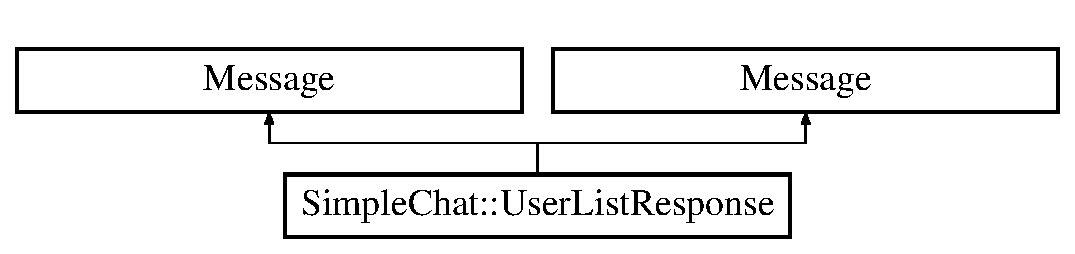
\includegraphics[height=2.000000cm]{classSimpleChat_1_1UserListResponse}
\end{center}
\end{figure}
\subsection*{Public Member Functions}
\begin{DoxyCompactItemize}
\item 
\hypertarget{classSimpleChat_1_1UserListResponse_a16b237391d6a195da652a12d0a3dd81d}{{\bfseries User\-List\-Response} (const \hyperlink{classSimpleChat_1_1UserListResponse}{User\-List\-Response} \&from)}\label{classSimpleChat_1_1UserListResponse_a16b237391d6a195da652a12d0a3dd81d}

\item 
\hypertarget{classSimpleChat_1_1UserListResponse_a777dbe9b9136d3c4e661fd4dd4f977cd}{\hyperlink{classSimpleChat_1_1UserListResponse}{User\-List\-Response} \& {\bfseries operator=} (const \hyperlink{classSimpleChat_1_1UserListResponse}{User\-List\-Response} \&from)}\label{classSimpleChat_1_1UserListResponse_a777dbe9b9136d3c4e661fd4dd4f977cd}

\item 
\hypertarget{classSimpleChat_1_1UserListResponse_ab4b494abc5d4878a87c8103f0ad44728}{const \\*
\-::google\-::protobuf\-::\-Unknown\-Field\-Set \& {\bfseries unknown\-\_\-fields} () const }\label{classSimpleChat_1_1UserListResponse_ab4b494abc5d4878a87c8103f0ad44728}

\item 
\hypertarget{classSimpleChat_1_1UserListResponse_a506a12daf50705b94c187981afa036e6}{inline\-::google\-::protobuf\-::\-Unknown\-Field\-Set $\ast$ {\bfseries mutable\-\_\-unknown\-\_\-fields} ()}\label{classSimpleChat_1_1UserListResponse_a506a12daf50705b94c187981afa036e6}

\item 
\hypertarget{classSimpleChat_1_1UserListResponse_a68d71246e15fdb6e36bb3d3858d512ed}{void {\bfseries Swap} (\hyperlink{classSimpleChat_1_1UserListResponse}{User\-List\-Response} $\ast$other)}\label{classSimpleChat_1_1UserListResponse_a68d71246e15fdb6e36bb3d3858d512ed}

\item 
\hypertarget{classSimpleChat_1_1UserListResponse_a8369b7418d0b9f0ce0bbff3805fe5e8f}{\hyperlink{classSimpleChat_1_1UserListResponse}{User\-List\-Response} $\ast$ {\bfseries New} () const }\label{classSimpleChat_1_1UserListResponse_a8369b7418d0b9f0ce0bbff3805fe5e8f}

\item 
\hypertarget{classSimpleChat_1_1UserListResponse_a25678c10520af6c57f02e689298f7555}{\hyperlink{classSimpleChat_1_1UserListResponse}{User\-List\-Response} $\ast$ {\bfseries New} (\-::google\-::protobuf\-::\-Arena $\ast$arena) const }\label{classSimpleChat_1_1UserListResponse_a25678c10520af6c57f02e689298f7555}

\item 
\hypertarget{classSimpleChat_1_1UserListResponse_af4f196b33d7cde3cbc29e5b4aca712b4}{void {\bfseries Copy\-From} (const \-::google\-::protobuf\-::\-Message \&from)}\label{classSimpleChat_1_1UserListResponse_af4f196b33d7cde3cbc29e5b4aca712b4}

\item 
\hypertarget{classSimpleChat_1_1UserListResponse_a2debc0c0b90687b53970c24f2eb2ea0e}{void {\bfseries Merge\-From} (const \-::google\-::protobuf\-::\-Message \&from)}\label{classSimpleChat_1_1UserListResponse_a2debc0c0b90687b53970c24f2eb2ea0e}

\item 
\hypertarget{classSimpleChat_1_1UserListResponse_a4f43f27a16728fb3e316123c4c181892}{void {\bfseries Copy\-From} (const \hyperlink{classSimpleChat_1_1UserListResponse}{User\-List\-Response} \&from)}\label{classSimpleChat_1_1UserListResponse_a4f43f27a16728fb3e316123c4c181892}

\item 
\hypertarget{classSimpleChat_1_1UserListResponse_aa4ab8470fb47c0c792b6950efea555e7}{void {\bfseries Merge\-From} (const \hyperlink{classSimpleChat_1_1UserListResponse}{User\-List\-Response} \&from)}\label{classSimpleChat_1_1UserListResponse_aa4ab8470fb47c0c792b6950efea555e7}

\item 
\hypertarget{classSimpleChat_1_1UserListResponse_a8b34e9384998f73e4edc7956925566d7}{void {\bfseries Clear} ()}\label{classSimpleChat_1_1UserListResponse_a8b34e9384998f73e4edc7956925566d7}

\item 
\hypertarget{classSimpleChat_1_1UserListResponse_a062c71b80549b7ec68d7d53c7a4c4b26}{bool {\bfseries Is\-Initialized} () const }\label{classSimpleChat_1_1UserListResponse_a062c71b80549b7ec68d7d53c7a4c4b26}

\item 
\hypertarget{classSimpleChat_1_1UserListResponse_af8d8db17515cc8a05428636db1667f33}{int {\bfseries Byte\-Size} () const }\label{classSimpleChat_1_1UserListResponse_af8d8db17515cc8a05428636db1667f33}

\item 
\hypertarget{classSimpleChat_1_1UserListResponse_a070121c5d035b79d64ef1c1d4478a667}{bool {\bfseries Merge\-Partial\-From\-Coded\-Stream} (\-::google\-::protobuf\-::io\-::\-Coded\-Input\-Stream $\ast$input)}\label{classSimpleChat_1_1UserListResponse_a070121c5d035b79d64ef1c1d4478a667}

\item 
\hypertarget{classSimpleChat_1_1UserListResponse_ad482db6ecf83a8774585d6c61d3c26ab}{void {\bfseries Serialize\-With\-Cached\-Sizes} (\-::google\-::protobuf\-::io\-::\-Coded\-Output\-Stream $\ast$output) const }\label{classSimpleChat_1_1UserListResponse_ad482db6ecf83a8774585d6c61d3c26ab}

\item 
\hypertarget{classSimpleChat_1_1UserListResponse_a9b075ee40113e581b5cc7bddfbb392b3}{\-::google\-::protobuf\-::uint8 $\ast$ {\bfseries Serialize\-With\-Cached\-Sizes\-To\-Array} (\-::google\-::protobuf\-::uint8 $\ast$output) const }\label{classSimpleChat_1_1UserListResponse_a9b075ee40113e581b5cc7bddfbb392b3}

\item 
\hypertarget{classSimpleChat_1_1UserListResponse_a9ffec135df81b1161c04402e083e67c2}{int {\bfseries Get\-Cached\-Size} () const }\label{classSimpleChat_1_1UserListResponse_a9ffec135df81b1161c04402e083e67c2}

\item 
\hypertarget{classSimpleChat_1_1UserListResponse_ac52be5912c5abdf036f561b110653a0d}{\-::google\-::protobuf\-::\-Metadata {\bfseries Get\-Metadata} () const }\label{classSimpleChat_1_1UserListResponse_ac52be5912c5abdf036f561b110653a0d}

\item 
\hypertarget{classSimpleChat_1_1UserListResponse_a160638ddfd252c614f2d198a77de1432}{int {\bfseries users\-\_\-size} () const }\label{classSimpleChat_1_1UserListResponse_a160638ddfd252c614f2d198a77de1432}

\item 
\hypertarget{classSimpleChat_1_1UserListResponse_ac2ba064ef33346bb6d93d7a3d0b160d1}{void {\bfseries clear\-\_\-users} ()}\label{classSimpleChat_1_1UserListResponse_ac2ba064ef33346bb6d93d7a3d0b160d1}

\item 
\hypertarget{classSimpleChat_1_1UserListResponse_a0247d22d738ad333bde0e4aad4fd388a}{const \-::\hyperlink{classSimpleChat_1_1User}{Simple\-Chat\-::\-User} \& {\bfseries users} (int index) const }\label{classSimpleChat_1_1UserListResponse_a0247d22d738ad333bde0e4aad4fd388a}

\item 
\hypertarget{classSimpleChat_1_1UserListResponse_a639e3b290026f8006abcc10ead90602c}{\-::\hyperlink{classSimpleChat_1_1User}{Simple\-Chat\-::\-User} $\ast$ {\bfseries mutable\-\_\-users} (int index)}\label{classSimpleChat_1_1UserListResponse_a639e3b290026f8006abcc10ead90602c}

\item 
\hypertarget{classSimpleChat_1_1UserListResponse_a56733ab0111a49c82b71fe7d7aa64046}{\-::\hyperlink{classSimpleChat_1_1User}{Simple\-Chat\-::\-User} $\ast$ {\bfseries add\-\_\-users} ()}\label{classSimpleChat_1_1UserListResponse_a56733ab0111a49c82b71fe7d7aa64046}

\item 
\hypertarget{classSimpleChat_1_1UserListResponse_a20d4c952b1341d25eb76e1517e70a13a}{\-::google\-::protobuf\-::\-Repeated\-Ptr\-Field\\*
$<$ \-::\hyperlink{classSimpleChat_1_1User}{Simple\-Chat\-::\-User} $>$ $\ast$ {\bfseries mutable\-\_\-users} ()}\label{classSimpleChat_1_1UserListResponse_a20d4c952b1341d25eb76e1517e70a13a}

\item 
\hypertarget{classSimpleChat_1_1UserListResponse_a81831bc5f06e11b3b720c771d7118b44}{const \\*
\-::google\-::protobuf\-::\-Repeated\-Ptr\-Field\\*
$<$ \-::\hyperlink{classSimpleChat_1_1User}{Simple\-Chat\-::\-User} $>$ \& {\bfseries users} () const }\label{classSimpleChat_1_1UserListResponse_a81831bc5f06e11b3b720c771d7118b44}

\item 
\hypertarget{classSimpleChat_1_1UserListResponse_a93a29d2d451637e32629f75afc14a1d3}{bool {\bfseries has\-\_\-message} () const }\label{classSimpleChat_1_1UserListResponse_a93a29d2d451637e32629f75afc14a1d3}

\item 
\hypertarget{classSimpleChat_1_1UserListResponse_a1fb116fab6ed4d52dfdd1387bf2a00ea}{void {\bfseries clear\-\_\-message} ()}\label{classSimpleChat_1_1UserListResponse_a1fb116fab6ed4d52dfdd1387bf2a00ea}

\item 
\hypertarget{classSimpleChat_1_1UserListResponse_a89f73b95a46ec8a5673311522f0e67c1}{const \-::std\-::string \& {\bfseries message} () const }\label{classSimpleChat_1_1UserListResponse_a89f73b95a46ec8a5673311522f0e67c1}

\item 
\hypertarget{classSimpleChat_1_1UserListResponse_a38821ca5b5905b782636898f01b602d4}{void {\bfseries set\-\_\-message} (const \-::std\-::string \&value)}\label{classSimpleChat_1_1UserListResponse_a38821ca5b5905b782636898f01b602d4}

\item 
\hypertarget{classSimpleChat_1_1UserListResponse_ac00038f982b13b4568282c6f0191e30b}{void {\bfseries set\-\_\-message} (const char $\ast$value)}\label{classSimpleChat_1_1UserListResponse_ac00038f982b13b4568282c6f0191e30b}

\item 
\hypertarget{classSimpleChat_1_1UserListResponse_ae44dc970456d556259264ebdbe9f2727}{void {\bfseries set\-\_\-message} (const char $\ast$value, size\-\_\-t size)}\label{classSimpleChat_1_1UserListResponse_ae44dc970456d556259264ebdbe9f2727}

\item 
\hypertarget{classSimpleChat_1_1UserListResponse_a520f406aea09996614aa68d87b3d91fc}{\-::std\-::string $\ast$ {\bfseries mutable\-\_\-message} ()}\label{classSimpleChat_1_1UserListResponse_a520f406aea09996614aa68d87b3d91fc}

\item 
\hypertarget{classSimpleChat_1_1UserListResponse_a3ca109406363b8acb93fc2619e90efb4}{\-::std\-::string $\ast$ {\bfseries release\-\_\-message} ()}\label{classSimpleChat_1_1UserListResponse_a3ca109406363b8acb93fc2619e90efb4}

\item 
\hypertarget{classSimpleChat_1_1UserListResponse_aa30eaf3be3fdf6dc90d8c5afaf943caf}{void {\bfseries set\-\_\-allocated\-\_\-message} (\-::std\-::string $\ast$message)}\label{classSimpleChat_1_1UserListResponse_aa30eaf3be3fdf6dc90d8c5afaf943caf}

\item 
\hypertarget{classSimpleChat_1_1UserListResponse_a16b237391d6a195da652a12d0a3dd81d}{{\bfseries User\-List\-Response} (const \hyperlink{classSimpleChat_1_1UserListResponse}{User\-List\-Response} \&from)}\label{classSimpleChat_1_1UserListResponse_a16b237391d6a195da652a12d0a3dd81d}

\item 
\hypertarget{classSimpleChat_1_1UserListResponse_a777dbe9b9136d3c4e661fd4dd4f977cd}{\hyperlink{classSimpleChat_1_1UserListResponse}{User\-List\-Response} \& {\bfseries operator=} (const \hyperlink{classSimpleChat_1_1UserListResponse}{User\-List\-Response} \&from)}\label{classSimpleChat_1_1UserListResponse_a777dbe9b9136d3c4e661fd4dd4f977cd}

\item 
\hypertarget{classSimpleChat_1_1UserListResponse_ab4b494abc5d4878a87c8103f0ad44728}{const \\*
\-::google\-::protobuf\-::\-Unknown\-Field\-Set \& {\bfseries unknown\-\_\-fields} () const }\label{classSimpleChat_1_1UserListResponse_ab4b494abc5d4878a87c8103f0ad44728}

\item 
\hypertarget{classSimpleChat_1_1UserListResponse_a506a12daf50705b94c187981afa036e6}{inline\-::google\-::protobuf\-::\-Unknown\-Field\-Set $\ast$ {\bfseries mutable\-\_\-unknown\-\_\-fields} ()}\label{classSimpleChat_1_1UserListResponse_a506a12daf50705b94c187981afa036e6}

\item 
\hypertarget{classSimpleChat_1_1UserListResponse_a68d71246e15fdb6e36bb3d3858d512ed}{void {\bfseries Swap} (\hyperlink{classSimpleChat_1_1UserListResponse}{User\-List\-Response} $\ast$other)}\label{classSimpleChat_1_1UserListResponse_a68d71246e15fdb6e36bb3d3858d512ed}

\item 
\hypertarget{classSimpleChat_1_1UserListResponse_a8369b7418d0b9f0ce0bbff3805fe5e8f}{\hyperlink{classSimpleChat_1_1UserListResponse}{User\-List\-Response} $\ast$ {\bfseries New} () const }\label{classSimpleChat_1_1UserListResponse_a8369b7418d0b9f0ce0bbff3805fe5e8f}

\item 
\hypertarget{classSimpleChat_1_1UserListResponse_a25678c10520af6c57f02e689298f7555}{\hyperlink{classSimpleChat_1_1UserListResponse}{User\-List\-Response} $\ast$ {\bfseries New} (\-::google\-::protobuf\-::\-Arena $\ast$arena) const }\label{classSimpleChat_1_1UserListResponse_a25678c10520af6c57f02e689298f7555}

\item 
\hypertarget{classSimpleChat_1_1UserListResponse_af4f196b33d7cde3cbc29e5b4aca712b4}{void {\bfseries Copy\-From} (const \-::google\-::protobuf\-::\-Message \&from)}\label{classSimpleChat_1_1UserListResponse_af4f196b33d7cde3cbc29e5b4aca712b4}

\item 
\hypertarget{classSimpleChat_1_1UserListResponse_a2debc0c0b90687b53970c24f2eb2ea0e}{void {\bfseries Merge\-From} (const \-::google\-::protobuf\-::\-Message \&from)}\label{classSimpleChat_1_1UserListResponse_a2debc0c0b90687b53970c24f2eb2ea0e}

\item 
\hypertarget{classSimpleChat_1_1UserListResponse_a4f43f27a16728fb3e316123c4c181892}{void {\bfseries Copy\-From} (const \hyperlink{classSimpleChat_1_1UserListResponse}{User\-List\-Response} \&from)}\label{classSimpleChat_1_1UserListResponse_a4f43f27a16728fb3e316123c4c181892}

\item 
\hypertarget{classSimpleChat_1_1UserListResponse_aa4ab8470fb47c0c792b6950efea555e7}{void {\bfseries Merge\-From} (const \hyperlink{classSimpleChat_1_1UserListResponse}{User\-List\-Response} \&from)}\label{classSimpleChat_1_1UserListResponse_aa4ab8470fb47c0c792b6950efea555e7}

\item 
\hypertarget{classSimpleChat_1_1UserListResponse_a8b34e9384998f73e4edc7956925566d7}{void {\bfseries Clear} ()}\label{classSimpleChat_1_1UserListResponse_a8b34e9384998f73e4edc7956925566d7}

\item 
\hypertarget{classSimpleChat_1_1UserListResponse_a062c71b80549b7ec68d7d53c7a4c4b26}{bool {\bfseries Is\-Initialized} () const }\label{classSimpleChat_1_1UserListResponse_a062c71b80549b7ec68d7d53c7a4c4b26}

\item 
\hypertarget{classSimpleChat_1_1UserListResponse_af8d8db17515cc8a05428636db1667f33}{int {\bfseries Byte\-Size} () const }\label{classSimpleChat_1_1UserListResponse_af8d8db17515cc8a05428636db1667f33}

\item 
\hypertarget{classSimpleChat_1_1UserListResponse_a070121c5d035b79d64ef1c1d4478a667}{bool {\bfseries Merge\-Partial\-From\-Coded\-Stream} (\-::google\-::protobuf\-::io\-::\-Coded\-Input\-Stream $\ast$input)}\label{classSimpleChat_1_1UserListResponse_a070121c5d035b79d64ef1c1d4478a667}

\item 
\hypertarget{classSimpleChat_1_1UserListResponse_ad482db6ecf83a8774585d6c61d3c26ab}{void {\bfseries Serialize\-With\-Cached\-Sizes} (\-::google\-::protobuf\-::io\-::\-Coded\-Output\-Stream $\ast$output) const }\label{classSimpleChat_1_1UserListResponse_ad482db6ecf83a8774585d6c61d3c26ab}

\item 
\hypertarget{classSimpleChat_1_1UserListResponse_a9b075ee40113e581b5cc7bddfbb392b3}{\-::google\-::protobuf\-::uint8 $\ast$ {\bfseries Serialize\-With\-Cached\-Sizes\-To\-Array} (\-::google\-::protobuf\-::uint8 $\ast$output) const }\label{classSimpleChat_1_1UserListResponse_a9b075ee40113e581b5cc7bddfbb392b3}

\item 
\hypertarget{classSimpleChat_1_1UserListResponse_a9ffec135df81b1161c04402e083e67c2}{int {\bfseries Get\-Cached\-Size} () const }\label{classSimpleChat_1_1UserListResponse_a9ffec135df81b1161c04402e083e67c2}

\item 
\hypertarget{classSimpleChat_1_1UserListResponse_ac52be5912c5abdf036f561b110653a0d}{\-::google\-::protobuf\-::\-Metadata {\bfseries Get\-Metadata} () const }\label{classSimpleChat_1_1UserListResponse_ac52be5912c5abdf036f561b110653a0d}

\item 
\hypertarget{classSimpleChat_1_1UserListResponse_a160638ddfd252c614f2d198a77de1432}{int {\bfseries users\-\_\-size} () const }\label{classSimpleChat_1_1UserListResponse_a160638ddfd252c614f2d198a77de1432}

\item 
\hypertarget{classSimpleChat_1_1UserListResponse_ac2ba064ef33346bb6d93d7a3d0b160d1}{void {\bfseries clear\-\_\-users} ()}\label{classSimpleChat_1_1UserListResponse_ac2ba064ef33346bb6d93d7a3d0b160d1}

\item 
\hypertarget{classSimpleChat_1_1UserListResponse_a2312720f3fb98c86b17ef0b54af15962}{const \-::\hyperlink{classSimpleChat_1_1User}{Simple\-Chat\-::\-User} \& {\bfseries users} (int index) const }\label{classSimpleChat_1_1UserListResponse_a2312720f3fb98c86b17ef0b54af15962}

\item 
\hypertarget{classSimpleChat_1_1UserListResponse_ab0a525717ebe79521d61e4d458756060}{\-::\hyperlink{classSimpleChat_1_1User}{Simple\-Chat\-::\-User} $\ast$ {\bfseries mutable\-\_\-users} (int index)}\label{classSimpleChat_1_1UserListResponse_ab0a525717ebe79521d61e4d458756060}

\item 
\hypertarget{classSimpleChat_1_1UserListResponse_a3bda6ae47efe16e37585b80364f46ef7}{\-::\hyperlink{classSimpleChat_1_1User}{Simple\-Chat\-::\-User} $\ast$ {\bfseries add\-\_\-users} ()}\label{classSimpleChat_1_1UserListResponse_a3bda6ae47efe16e37585b80364f46ef7}

\item 
\hypertarget{classSimpleChat_1_1UserListResponse_af8612ce1fc3c9b9e745e8e67ab2be3d0}{\-::google\-::protobuf\-::\-Repeated\-Ptr\-Field\\*
$<$ \-::\hyperlink{classSimpleChat_1_1User}{Simple\-Chat\-::\-User} $>$ $\ast$ {\bfseries mutable\-\_\-users} ()}\label{classSimpleChat_1_1UserListResponse_af8612ce1fc3c9b9e745e8e67ab2be3d0}

\item 
\hypertarget{classSimpleChat_1_1UserListResponse_a5385a14ac8d32845f66ed5f46e35e8e3}{const \\*
\-::google\-::protobuf\-::\-Repeated\-Ptr\-Field\\*
$<$ \-::\hyperlink{classSimpleChat_1_1User}{Simple\-Chat\-::\-User} $>$ \& {\bfseries users} () const }\label{classSimpleChat_1_1UserListResponse_a5385a14ac8d32845f66ed5f46e35e8e3}

\item 
\hypertarget{classSimpleChat_1_1UserListResponse_a93a29d2d451637e32629f75afc14a1d3}{bool {\bfseries has\-\_\-message} () const }\label{classSimpleChat_1_1UserListResponse_a93a29d2d451637e32629f75afc14a1d3}

\item 
\hypertarget{classSimpleChat_1_1UserListResponse_a1fb116fab6ed4d52dfdd1387bf2a00ea}{void {\bfseries clear\-\_\-message} ()}\label{classSimpleChat_1_1UserListResponse_a1fb116fab6ed4d52dfdd1387bf2a00ea}

\item 
\hypertarget{classSimpleChat_1_1UserListResponse_affadf6bc4bc13acda51cb898827620d1}{const \-::std\-::string \& {\bfseries message} () const }\label{classSimpleChat_1_1UserListResponse_affadf6bc4bc13acda51cb898827620d1}

\item 
\hypertarget{classSimpleChat_1_1UserListResponse_a38821ca5b5905b782636898f01b602d4}{void {\bfseries set\-\_\-message} (const \-::std\-::string \&value)}\label{classSimpleChat_1_1UserListResponse_a38821ca5b5905b782636898f01b602d4}

\item 
\hypertarget{classSimpleChat_1_1UserListResponse_ac00038f982b13b4568282c6f0191e30b}{void {\bfseries set\-\_\-message} (const char $\ast$value)}\label{classSimpleChat_1_1UserListResponse_ac00038f982b13b4568282c6f0191e30b}

\item 
\hypertarget{classSimpleChat_1_1UserListResponse_ae44dc970456d556259264ebdbe9f2727}{void {\bfseries set\-\_\-message} (const char $\ast$value, size\-\_\-t size)}\label{classSimpleChat_1_1UserListResponse_ae44dc970456d556259264ebdbe9f2727}

\item 
\hypertarget{classSimpleChat_1_1UserListResponse_abff2add13917ba30b545589db20940c5}{\-::std\-::string $\ast$ {\bfseries mutable\-\_\-message} ()}\label{classSimpleChat_1_1UserListResponse_abff2add13917ba30b545589db20940c5}

\item 
\hypertarget{classSimpleChat_1_1UserListResponse_a9129ebcc182957a755bae9b238406035}{\-::std\-::string $\ast$ {\bfseries release\-\_\-message} ()}\label{classSimpleChat_1_1UserListResponse_a9129ebcc182957a755bae9b238406035}

\item 
\hypertarget{classSimpleChat_1_1UserListResponse_aa30eaf3be3fdf6dc90d8c5afaf943caf}{void {\bfseries set\-\_\-allocated\-\_\-message} (\-::std\-::string $\ast$message)}\label{classSimpleChat_1_1UserListResponse_aa30eaf3be3fdf6dc90d8c5afaf943caf}

\end{DoxyCompactItemize}
\subsection*{Static Public Member Functions}
\begin{DoxyCompactItemize}
\item 
\hypertarget{classSimpleChat_1_1UserListResponse_a86588d80967730a330fe8a1f66778122}{static const \\*
\-::google\-::protobuf\-::\-Descriptor $\ast$ {\bfseries descriptor} ()}\label{classSimpleChat_1_1UserListResponse_a86588d80967730a330fe8a1f66778122}

\item 
\hypertarget{classSimpleChat_1_1UserListResponse_ac44368ffc59e770e328d1418cd015201}{static const \hyperlink{classSimpleChat_1_1UserListResponse}{User\-List\-Response} \& {\bfseries default\-\_\-instance} ()}\label{classSimpleChat_1_1UserListResponse_ac44368ffc59e770e328d1418cd015201}

\item 
\hypertarget{classSimpleChat_1_1UserListResponse_a86588d80967730a330fe8a1f66778122}{static const \\*
\-::google\-::protobuf\-::\-Descriptor $\ast$ {\bfseries descriptor} ()}\label{classSimpleChat_1_1UserListResponse_a86588d80967730a330fe8a1f66778122}

\item 
\hypertarget{classSimpleChat_1_1UserListResponse_ac44368ffc59e770e328d1418cd015201}{static const \hyperlink{classSimpleChat_1_1UserListResponse}{User\-List\-Response} \& {\bfseries default\-\_\-instance} ()}\label{classSimpleChat_1_1UserListResponse_ac44368ffc59e770e328d1418cd015201}

\end{DoxyCompactItemize}
\subsection*{Static Public Attributes}
\begin{DoxyCompactItemize}
\item 
\hypertarget{classSimpleChat_1_1UserListResponse_a7dfc88b1d66d710bd51e1beda0e80a35}{static const int {\bfseries k\-Users\-Field\-Number} = 1}\label{classSimpleChat_1_1UserListResponse_a7dfc88b1d66d710bd51e1beda0e80a35}

\item 
\hypertarget{classSimpleChat_1_1UserListResponse_a969be1985ed6791849e0f41e4c7ce413}{static const int {\bfseries k\-Message\-Field\-Number} = 2}\label{classSimpleChat_1_1UserListResponse_a969be1985ed6791849e0f41e4c7ce413}

\end{DoxyCompactItemize}
\subsection*{Friends}
\begin{DoxyCompactItemize}
\item 
\hypertarget{classSimpleChat_1_1UserListResponse_a21c725e9955d4dda1abc79b117f57e76}{void {\bfseries protobuf\-\_\-\-Add\-Desc\-\_\-\-User\-\_\-2eproto} ()}\label{classSimpleChat_1_1UserListResponse_a21c725e9955d4dda1abc79b117f57e76}

\item 
\hypertarget{classSimpleChat_1_1UserListResponse_aadc83181f80ae5102c4449a54aef288e}{void {\bfseries protobuf\-\_\-\-Assign\-Desc\-\_\-\-User\-\_\-2eproto} ()}\label{classSimpleChat_1_1UserListResponse_aadc83181f80ae5102c4449a54aef288e}

\item 
\hypertarget{classSimpleChat_1_1UserListResponse_ac6d6bd3817a5978496745d793da7465f}{void {\bfseries protobuf\-\_\-\-Shutdown\-File\-\_\-\-User\-\_\-2eproto} ()}\label{classSimpleChat_1_1UserListResponse_ac6d6bd3817a5978496745d793da7465f}

\item 
\hypertarget{classSimpleChat_1_1UserListResponse_a21c725e9955d4dda1abc79b117f57e76}{void {\bfseries protobuf\-\_\-\-Add\-Desc\-\_\-\-User\-\_\-2eproto} ()}\label{classSimpleChat_1_1UserListResponse_a21c725e9955d4dda1abc79b117f57e76}

\item 
\hypertarget{classSimpleChat_1_1UserListResponse_aadc83181f80ae5102c4449a54aef288e}{void {\bfseries protobuf\-\_\-\-Assign\-Desc\-\_\-\-User\-\_\-2eproto} ()}\label{classSimpleChat_1_1UserListResponse_aadc83181f80ae5102c4449a54aef288e}

\item 
\hypertarget{classSimpleChat_1_1UserListResponse_ac6d6bd3817a5978496745d793da7465f}{void {\bfseries protobuf\-\_\-\-Shutdown\-File\-\_\-\-User\-\_\-2eproto} ()}\label{classSimpleChat_1_1UserListResponse_ac6d6bd3817a5978496745d793da7465f}

\end{DoxyCompactItemize}


The documentation for this class was generated from the following file\-:\begin{DoxyCompactItemize}
\item 
chatlib/proto/User.\-pb.\-h\end{DoxyCompactItemize}

%--- End generated contents ---

% Index
\newpage
\phantomsection
\addcontentsline{toc}{chapter}{Index}
\printindex

\end{document}
